%!TEX encoding = ISO-8859-1

\documentclass[11pt,a4paper,oneside,final]{memoir}

% packages:
\PassOptionsToPackage{obeyspaces,hyphens}{url}
\XeTeXinputencoding latin1
\usepackage[T1]{fontenc}
\usepackage[UKenglish]{isodate}
\usepackage[
	backend=biber,
	natbib=true,
	refsection=chapter,
	backref=false,
	hyperref=true,
	style=authoryear,
	citestyle=authoryear,
	sortcites,
	sorting=nyt,
	maxcitenames=2,
	uniquelist=false,
	uniquename=false,
	url=false,
	isbn=false,
	giveninits=true,
	useprefix=true,
	doi=false
]{biblatex}
\renewbibmacro{in:}{\ifentrytype{article}{}{\printtext{\bibstring{in}\intitlepunct}}}
\renewbibmacro*{volume+number+eid}{%
	\printfield{volume}%
	\setunit*{\addnbthinspace}
	\printfield{number}%
	\setunit{\addcomma\space}%
	\printfield{eid}}
\DeclareFieldFormat[article]{number}{\mkbibparens{#1}}
\usepackage{graphicx}
\usepackage{color}
\usepackage{tikz,pgf}
\usepackage{amsmath,amssymb,amsthm}
\usepackage[obeyspaces,hyphens]{url}
\usepackage{listings}
\usepackage{multirow}
\usepackage{booktabs}
\usepackage{xspace}
\usepackage{cancel}
\usepackage{subfig}
\usepackage[printonlyused,withpage]{acronym}
\usepackage{rotating}
\usepackage{array}
\usepackage[htt]{hyphenat}
\usepackage{setspace}
\usepackage{titlesec}
\usepackage[hang,flushmargin]{footmisc}
\usepackage{xfrac}
\usepackage{tabularx}
\usepackage{caption}
\usepackage{ragged2e}
\usepackage{xpatch}
\usepackage{bm, bbm, upgreek}
\usepackage[flushleft]{threeparttable}
\usepackage{ragged2e}
\usepackage{enumitem}
\usepackage{siunitx}
\usepackage{longtable}
\usepackage{threeparttablex}
\let\newfloat\undefined
\usepackage{floatrow}
\usepackage{wrapfig}
\usepackage{fontspec}
\usepackage{bbding}
\usepackage{pifont}
\usepackage{etoolbox}
\usepackage{letltxmacro}
\usepackage{geometry}
\usepackage{pdflscape}
\usepackage{titletoc}
\usepackage{chngcntr}
\usepackage{minitoc}
\def\myshorttitle{Publishing while female}
\def\mysubtitle{Are women held to higher standards? Evidence from peer review.}
\def\myauthor{Erin Hengel}
\def\myabstract{I use readability scores to test if women are held to higher standards in academic peer review. I find: (i) female-authored papers are 1--6 percent better written than equivalent papers by men; (ii) the gap is almost two times higher in the published articles than in the pre-print drafts (and no gap in papers subjected to double-blind review before the internet); (iii) women's writing gradually improves but men's does not---meaning the readability gap grows over authors' careers. Within a subjective expected utility framework, I exploit authors' decisions to show that tougher editorial standards and\slash or biased referee assignment are uniquely consistent with the observed pattern of choices. A conservative causal estimate derived from the model suggests senior female economists write at least 9 percent more clearly than they otherwise would. I then document evidence that higher standards affect behaviour and lower productivity. First, female-authored papers take half a year longer in peer review. Second, as women update beliefs about referees' standards, they increasingly meet those standards before peer review. The latter response disguises external thresholds as personal choice; the former reduces women's output. Both whitewash discrimination. More generally, tougher standards impose a quantity\slash quality tradeoff that characterises many instances of female output. They could resolve persistently lower---otherwise unexplained---female productivity in many high-skill occupations.}
\def\mydate{June 2018}
\def\address{Chatham Street, Liverpool L69 7ZH, U.K.}
\def\telephone{+44 (0)7 824 863 784}
\def\affiliation{University of Liverpool}
\def\department{Department of Economics}
\def\position{Lecturer in Economics}
\def\email{erin.hengel@liverpool.ac.uk}
\def\thanksbitches{This paper is a revised version of the third chapter of my dissertation (University of Cambridge, September 2015). I am grateful to my supervisor Christopher Harris for (a) excellent guidance and (b) thinking this was a good idea. I am similarly indebted to Jeremy Edwards and my examination committee (Leonardo Felli and Hamish Low) for considerable input and advice. I also thank Oriana Bandiera, Anne Boring, Cheryl Carleton, Gary Cook, Dominique Demougin, Harris Dellas, Carola Frege, Olga Gorelkina, Jane Hunt, John Leahy, Brendan McCabe, Reshef Meir, Imran Rasul, Ludovic Renou, Kevin Schnepel, Joel Sobel, Jarrod Zhang, audience members at the Econometric Society European Winter Meeting, the Eastern Economic Association Conference, the Royal Economic Society Annual Conference, the European Meeting of the Econometric Society, the American Economic Association Annual Meeting, the Review of Economics and Statistics Centenary Conference and seminar participants at the University of Liverpool and the University of Cardiff for useful comments. This paper could not have been written without substantial careful research assistance by Michael Hengel (my dad) and Eileen Hengel (my sister). All errors, of course, are mine.}
\def\keywords{gender, readability, discrimination}
\def\subject{Gender bias}
\def\jel{A11, J16, J24}
\def\wordcount{20,300}
% Set margins.
\geometry{
	a4paper,
	left=27mm,
	right=27mm,
	top=27mm,
	bottom=27mm
}

% Colors
\definecolor{webgreen}{rgb}{0, 0.5, 0}
\definecolor{boyblue}{rgb}{0.102, 0.157, 0.306}

% Bibliography.
\addbibresource{/Users/erinhengel/Dropbox/Readability/draft/0-bib/publishing_female.bib}
\addbibresource{/Users/erinhengel/Dropbox/Readability/draft/0-bib/online-appendix.bib}

\usepackage[	colorlinks=true,
				pdfstartpage=1,
				pdfstartview=FitV,
				pdfpagemode=FullScreen,
				bookmarksnumbered,
				hypertexnames=true,
				urlcolor=webgreen,
				anchorcolor=black,
				filecolor=black,
				menucolor=black,
				runcolor=webgreen,
				linkcolor=boyblue,
				citecolor=black,
				plainpages=false,
				pdfpagelabels,
				pdftitle={\myshorttitle},
				pdfauthor={\myauthor, \affiliation},
				pdfproducer={XeLaTeX},
				pdfcreator={LaTeX}
			]{hyperref}
\usepackage{appendix}
\usepackage{memhfixc}
\usepackage{fontspec}
\usepackage[capitalise]{cleveref}
\let\footruleskip\undefined
\usepackage{fancyhdr}
\usepackage{setspace}

% Fonts
\newcommand{\nfont}{Adobe Caslon Pro}
\newcommand{\ttfont}{Envy Code R}
\newcommand{\sffont}{Optima Regular}
\defaultfontfeatures{Mapping=tex-text}
\setromanfont[Ligatures={Common}]{\nfont}
\setmonofont[Scale=0.8]{\ttfont}
\setsansfont[Scale=0.9]{\sffont}

% Hypenations
\hyphenation{econ-omists}
\hyphenation{dum-my}
\hyphenation{a-g-ainst}
\hyphenation{work-outs}

% Set British date format.
\cleanlookdateon

% Paragraph spacing.
\def\myindent{1.5em}
\setlength{\parindent}{\myindent}

% Thanks footnote.
\makeatletter
	\def\thanksnote{\gdef\@thefnmark{}\@footnotetext}
\makeatother

% Footnote symbols.
\makeatletter
\renewcommand*{\@fnsymbol}[1]{\ensuremath{\ifcase#1\or *\or \dagger\or \ddagger\or
	\mathsection\or \mathparagraph\or \|\or **\or \dagger\dagger
	\or \ddagger\ddagger \else\@ctrerr\fi}}
\makeatother
\newenvironment{symfootnotes}{
	\par\edef\savedfootnotenumber{\number\value{footnote}}
	\renewcommand{\thefootnote}{\fnsymbol{footnote}}
	\setcounter{footnote}{0}}
	{\par\setcounter{footnote}{\savedfootnotenumber}
}

% Title page layout.
\makeatletter
	\title{\Large\myshorttitle\\\large\mysubtitle\footnote{\affiliation, \department, \address. Email: \href{mailto:\email}{\texttt{\email}}}
	\author{
		\myauthor\thanks{\thankyous}
	}\\\mydate
	}
	\renewcommand{\maketitle}{
		\bgroup
		\let\newpage\relax
		\begin{center}
			\begin{symfootnotes}
				\@title\\[0.5cm]
				\@author\@thanks\\\hfill
			\end{symfootnotes}
		\end{center}
		\egroup
	}
\makeatother

% Chapter style.
\makeatletter
	\makechapterstyle{paperbody}{

		% Section numering depth.
		\maxsecnumdepth{subsubsection}
	
		\renewcommand\thesection{\arabic{section}}
		\renewcommand\thesubsection{\thesection.\arabic{subsection}}
		\renewcommand\thechapter{\arabic{chapter}}

		% Section header formatting.
		\titleformat{\section}{\normalfont\large\bfseries}{\thesection}{1em}{}
		\titleformat{\subsection}{\normalfont\itshape}{\thesubsection}{1em}{}
		\titleformat{\subsubsection}[runin]{\normalfont\normalsize\bfseries}{\thesubsubsection}{1em}{\addperiod}
		\titleformat{\subsubsubsection}[runin]{\normalfont\normalsize\textit}{}{1em}{\addperiod}
		\titlespacing*{\paragraph}{\indent}{10pt}{0.4em}
		\titleformat{\paragraph}[runin]{\normalfont\normalsize\itshape}{}{0em}{\addperiod}
		\titlespacing*{\paragraph}{\myindent}{10pt}{0.4em}

		% Autoref.
		\renewcommand{\chapterautorefname}{Chapter}
		\renewcommand{\sectionautorefname}{Section}
		\renewcommand{\footnoteautorefname}{Footnote}
		\let\subsectionautorefname\sectionautorefname
		\let\subsubsectionautorefname\sectionautorefname
		\let\subsubsubsectionautorefname\sectionautorefname

		% Equation numbering (1), (2), ....
		\def\theequation{\thechapter.\arabic{equation}}
		\def\tagform@##1{\maketag@@@{\ignorespaces##1\unskip\@@italiccorr}}
		\renewcommand{\theequation}{(\arabic{equation})}

		% Figure numbering.
		\renewcommand{\thefigure}{\arabic{figure}}
		\renewcommand{\fnum@figure}{\textsc{Figure~\thefigure}}
	
		% Table numbering.
		\renewcommand{\thetable}{\arabic{table}}
	
		% Quote environment.
		\patchcmd{\quote}{\rightmargin}{\small\leftmargin 4em \rightmargin}{}{}
	
		\pagestyle{plain}
	}
\makeatother

% Appendix.
\AtBeginEnvironment{subappendices}{%
	\chapter*{Appendices}
}
\renewcommand{\setthesection}{\Alph{section}}

% Online appendix.
\renewenvironment{appendices}{%
	\renewcommand\appendixname{Online appendices}

	\clearpage
	\setcounter{subsection}{0}
	\begin{center}
		\Large\myshorttitle
		
		\large\myauthor
		
		\large\mydate
		
		\LARGE\textbf{\appendixname}
		
	\end{center}
	\vfill
	\renewcommand{\thesection}{\Alph{section}}
	\renewcommand{\thesubsection}{\Alph{section}.\arabic{subsection}}
	\renewcommand{\theequation}{(\thesection.\arabic{equation})}

	\pagenumbering{gobble}
	\startcontents[annexes]
	\printcontents[annexes]{l}{0}{\setcounter{tocdepth}{3}}
	\vfill
	\stopcontents[corpstexte]
	\clearpage
	\pagenumbering{arabic}

	\setcounter{footnote}{0}
	\setcounter{figure}{0}
	\setcounter{table}{0}
	\setcounter{equation}{0}
	\counterwithin*{table}{section}
	\counterwithin*{figure}{section}
	\counterwithin*{equation}{section}
	\renewcommand{\theequation}{(\thesection.\arabic{equation})}
	\renewcommand{\thetable}{\thesection.\arabic{table}}
	\renewcommand{\thefigure}{\thesection.\arabic{figure}}

	\pagenumbering{arabic}
	\setcounter{page}{1}
}{\setcounter{subsection}{0}}%

% Theorems, lemmas and corollaries.
\theoremstyle{plain}
\newtheorem{theorem}{Theorem}
\newtheorem{lemma}{Lemma}
\providecommand*{\lemmaautorefname}{Lemma}
\newtheorem{corollary}{Corollary}
\providecommand*{\corollaryautorefname}{Corollary}

% Table style.
\captionsetup[table]{
	position=top,
	justification=centering,
	labelfont=sc,
}
\renewcommand{\arraystretch}{1.1}
\sisetup{
	input-symbols = (),
	table-align-text-post = false,
	input-decimal-markers = {.},
	group-digits = integer,
	round-mode = places,
	round-precision = 2,
	tight-spacing = true,
	group-separator = {,},
	group-minimum-digits=4,
	table-format = 4.4,
}
\floatsetup[table]{capposition=top}

% Shortcut commands
\newcommand{\wt}{\widetilde}
\newcommand{\vect}[1]{\mathbf{#1}}
\newcommand{\mrow}[2]{\multirow{2}{*}{\parbox[t][1cm][t]{#1}{\raggedright #2}}}
\newcommand{\mcol}[1]{\multicolumn{6}{l}{#1}}
\newcommand{\vep}{\varepsilon}
\newcommand{\crcell}[2][c]{
	\begin{tabular}[#1]{@{}c@{}}#2\end{tabular}
}
\newcommand{\aref}[1]{\hyperref[#1]{Appendix~\ref{#1}}}
\newcolumntype{L}[1]{>{\raggedright\let\newline\\\arraybackslash\hspace{0pt}}m{#1}}

% Graphics path.
\graphicspath{{/Users/erinhengel/Dropbox/Readability/draft}}

% Gracphics rule.
\DeclareGraphicsRule{*}{pdf}{*}{}

\begin{document}
\mainmatter
\chapterstyle{paperbody}

\begin{vplace}[0.7]
	\maketitle
	\begin{quote}
		% This paper documents several stylised facts about gender, readability and review times in top economics journals: (i) female authors are very under-represented; (ii) their papers are better written; (iii) the gender gap in readability widens during peer review; (iv) women improve their writing as they publish more papers but men do not; (v) female-authored papers take longer under review. Using a subjective expected utility framework, I argue that these stylised facts are consistent with editors and/or referees applying higher standards to women's writing. A counterfactual analysis suggests senior female economists may, as a result, write at least five percent more clearly than they otherwise would. As a final exercise, I show tentative evidence that women adapt to biased treatment in ways that may disguise it as voluntary choice.


Female authors are underrepresented in top economics journals. In this paper, I investigate whether higher writing standards contribute to the problem. I find: (i) female-authored papers are 1--6 percent better written than equivalent papers by men; (ii) the gap widens during peer review; (iii) women improve their writing as they publish more papers (but men do not); (iv) female-authored papers take longer under review. Using a subjective expected utility framework, I argue that higher writing standards for women are consistent with these stylised facts. A counterfactual analysis suggests senior female economists may, as a result, write at least five percent more clearly than they otherwise would. As a final exercise, I show tentative evidence that women adapt to biased treatment in ways that may disguise it as voluntary choice.
		
		Keywords. \keywords
		
		\textit{JEL} codes. \jel
	\end{quote}
\end{vplace}
\thispagestyle{empty}
\clearpage

\pagenumbering{gobble}
\pagenumbering{arabic}


\section{Introduction}
\label{introduction}

Female economists are less likely to make tenure, take longer when they do and earn much less than their male peers~\citep{Bandiera2016,Ceci2014,Ginther2004,Weisshaar2017}.\footnote{\citet{Weisshaar2017} evaluates the probability of making tenure in Sociology, Computer Science and English departments.} Only a third, fifth and tenth of assistant, associate and full professors, respectively, are women~\citep{Romero2013}. We make up just 14 percent of authors published in top economics journals since 2000.

These statistics are uncomfortable, but their causes are myriad: lower publishing rates, career choices, motherhood and, probably, bias. In lab experiments women are subject to tougher standards. Their qualifications and ability are underestimated~\citep{Foschi1996,Grunspan2016,Moss-Racusin2012,Reuben2014}. Female-authored manu\-scripts are evaluated more critically~\citep{Goldberg1968,Krawczyk2016,Paludi1983}; when collaborating with men, women are given less credit~\citep{Heilman2005,Sarsons2015}.

This paper uses five reliable measures of writing clarity to show that women are likewise held to higher standards in peer review. (i) Female-authored articles published in top economics journals are better written than similar papers by men. The difference cannot be explained by year, journal, editor, topic, institution, English language ability or with various proxies for article quality and author productivity. (ii) The gap widens precisely while papers are being reviewed. I compare published articles to their pre-reviewed drafts. Forty percent of the gap originates \emph{during} peer review. Moreover, there is no evidence of a gap in papers subjected to double-blind review before the internet. (iii) Female economists improve their writing; male economists don't. A dynamic model of an author's decision-making process shows that tougher editorial standards and\slash or biased referee assignment are the only explanations consistent with women's choices. Using a conservative measure derived from the model, I estimate that this type of discrimination causes senior female economists to write at least 9 percent more clearly than they otherwise would.

I also document evidence that higher standards confound productivity measurement and their own identification. First, higher standards presumably delay review---and as anticipated, female-authored papers spend six months longer in peer review. This estimate is based on submit-accept times at \emph{Econometrica}, and controls for, \emph{inter alia}, motherhood, childbirth, citations and field. Second, women adjust to biased treatment in ways that partially---or even totally---confuse it with voluntary choice. Although the readability gap rises with experience, the portion formed in peer review falls. Studies that analyse only this trajectory may underestimate discrimination, misallocate responsibility or even conclude bias against men.

Higher standards impose a quantity\slash quality tradeoff that likely contributes to academia's ``Publishing Paradox'' and ``Leaky Pipeline''.\footnote{``Publishing Paradox'' and ``Leaky Pipeline'' refer to phenomena in academia whereby women publish fewer papers and disproportionately leave the profession, respectively.} Spending more time revising old research means there's less time for new research. Fewer papers results in fewer promotions, possibly driving women into fairer fields. Moreover, evidence of this tradeoff is present in a variety of occupations---\emph{e.g.}, doctors, real estate agents and airline pilots---suggesting higher standards distort women's productivity, more generally.

\vspace*{\baselineskip}

Prior research indicates journal acceptance rates are genuinely bias-free ~\citep[see, \emph{e.g.},][]{Blank1991,Borsuk2009,Gilbert1994}.\footnote{A possible exception is \emph{Behavioral Ecology}, which increased its number of female first-authored papers after switching to double-blind review in 2001~\citep{Budden2008a}. Whether that increase was due to bias or the universal upward trend in female authorship, however, has been somewhat controversial~\citep{Budden2008b,Budden2008c,Webb2008,Whittaker2008}.} To the best of my knowledge, however, gender neutrality is established in only a narrow context (publication outcomes) using this single indicator. I ask a different question. Men's and women's papers may be published at comparable \emph{rates}, but are they reviewed with comparable \emph{scrutiny}? For, if women are stereotypically assumed less capable at math, logic and reasoning than men and generally need more evidence to rate as equally competent, some well-intentioned referees might (unknowingly) inspect their papers more closely, demand a larger number of revisions and, in general, be less tolerant of complicated, dense writing.

Complicated, dense writing is my focus. In the English language, more clearly written prose is better prose, all things equal. Thoughtful word choice and simple sentence structure make text easier to understand, more interesting to read and expose inconsistencies long-winded writing often hides. Journal editors tend to agree---\emph{Econometrica} asks authors to write ``crisply but clearly'' and to take ``the extra effort involved in revising and reworking the manuscript until it will be clear to most if not all of our readers'' (\href{http://www.econometricsociety.org/publications/econometrica/information-authors/instructions-submitting-articles}{\emph{Econometrica} submission guidelines}, June 2016).\footnote{The \emph{American Economic Review} rejected Robert Lucas's paper ``Expectations and the Neutrality of Money'' for insufficient readability; one referee wrote ``If it has a clear result, it is hidden by the exposition''~\citep[][p. 172]{Gans1994}. In a random selection of 100 posts on \href{http://shitmyreviewerssay.tumblr.com/submit}{Shit My Reviewers Say}, a quarter deal with writing quality, document structure or word choice\slash tone.}

If referees hold female- and male-authored papers to identical standards, both should be equally well written. To test this, I rely on a relationship familiar to linguists and educators: simple vocabulary and short sentences are easier to understand and straightforward to quantify. Using the five most widely used, studied and reliable formulas to exploit this, I analyse 9,123 article abstracts\footnote{Readability scores are highly correlated across an article's abstract, introduction and discussion sections~\citep{Hartley2003a}. See \autoref{data} for further discussion.} published in the \emph{American Economic Review} (\emph{AER}), \emph{Econometrica} (\emph{ECA}), \emph{Journal of Political Economy} (\emph{JPE}) and \emph{Quarterly Journal of Economics} (\emph{QJE}).\footnote{For a discussion on the reliability of readability formulas, see  \citet{DuBay2004} and \autoref{measuringreadability}. A sixth commonly used measure is the Lexile Framework. Because its formula and software are proprietary, I do not include it in the analysis.}

Female-authored abstracts are 1--6 percent more readable than those by men. Women write better despite controls for editor, journal, year and primary and tertiary \emph{JEL} classification; that remains unchanged when proxying for article and author quality or accounting for English fluency. This means the readability gap probably wasn't (i) a response to specific policies in earlier eras; (ii) caused by women writing on topics that are easier to explain; (iii) due to a lopsided concentration of (non-)native English speakers;\footnote{It is not clear how---or even if---native English speakers write more clearly than non-native speakers. In fact, \citet{Hayden2008} found that peer reviewed articles by the latter are more readable, on average.} nor (iv) generated by factors correlated with gender but really related to knowledge, intelligence and creativity.

Additionally, the gender readability gap widens \emph{during} peer review. I compare National Bureau of Economic Research (NBER) working papers to their final, published versions; the gap is almost twice as large for the latter.\footnote{Many thanks to Kevin Schnepel for suggesting this idea.} While both papers are exposed to many factors that impact readability, only published articles are subject to peer review. By comparing the two, influences unrelated to immediate peer review are isolated from those that are; assuming the former are not correlated with the latter's timing, a widening gap suggests a causal link. Consistent with this hypothesis, I also find no evidence of a gender readability gap in the (small) number of articles subjected to double-blind peer review before the internet.

Revising, redrafting and selecting just the right word is hard work; making sentences even marginally more readable takes time. Consistent with this hypothesis, I find female-authored papers spend \textbf{\emph{six months longer}} in peer review. This estimate is based on submit-accept times from \emph{Econometrica}, persists across a range of specifications and, in addition to other factors, controls for motherhood, childbirth, citations and field.\footnote{Predictably, giving birth slows down peer review. The coefficient on motherhood, however, is consistently negative (indicating a productivity boost) and almost always highly significant when subjected to several robustness checks. This result is provocative and discussed in \autoref{duration}. I encourage interpreting it with caution, however, given (i) counterintuitive results; (ii) the analysis did not intend to measure motherhood's impact on review times; and especially (iii) only a small number of mothers with young children are published in \emph{Econometrica}.}

Two explanations could account for these findings: either women voluntarily write better papers---\emph{e.g.}, because they're more sensitive to referee criticism or overestimate the importance of writing well---or better written papers are women's response to external thresholds they do not control. Both imply women spend too much time rewriting old papers and not enough time writing new papers---but my evidence suggests the latter is primarily to blame.

In a dynamic model of an author's decision making process, I show that if women improve their writing over time and are not commensurately rewarded with higher acceptance rates (relative to men), then a persistent readability gap between equivalent peers is caused by discrimination. Authors improve readability only if they believe better writing leads to higher acceptance rates. And while oversensitivity and\slash or poor information may distort their beliefs---and affect readability---the impact declines with experience. Holding acceptance rates constant, this implies that a widening readability gap between equivalent authors is caused by discrimination---\emph{i.e.}, asymmetric editorial standards and\slash or biased referee assignment beyond their control (\autoref{Theorem1}).

\autoref{Theorem1} establishes sufficient conditions to demonstrate double standards are present in academic publishing: (i) experienced women write better than experienced men; (ii) women improve their writing over time; (iii) female-authored papers are accepted no more often than male-authored papers. Estimates from pooled subsamples at fixed publication counts suggest (i) and (ii) hold. On average, women's writing gradually gets better but men's does not. Between authors' first and third published articles, the readability gap increases by up to 12 percent. Although my data do not identify probability of acceptance, conclusions from extensive study elsewhere are clear: ``there are no sex differences in acceptance rates.''~\citep[][p. 111; see also \autoref{seumatching} for references to other research supporting this claim]{Ceci2014}.

I also match prolific female authors to similarly productive male authors on characteristics that predict the topic, novelty and quality of research. In addition to explicitly accounting for author equivalence---the (principle) conditional independence assumption behind \autoref{Theorem1}---matched pair comparisons: (i) identify the gender most likely to satisfy \autoref{Theorem1}`s conditions simultaneously;\footnote{Each of \autoref{Theorem1}'s conditions must technically hold for the same author in two different situations---before and after gaining experience and when compared to an equivalent, experienced author of the opposite gender.} and (ii) generate a (conservative) estimate of the effect of higher standards on authors' readability (\autoref{Corollary1}).

\autoref{Theorem1}'s conditions were satisfied in 65 percent of matched pairs. In three quarters of those, the member discriminated against was female. Moreover, instances of obvious discrimination were predominately against women: the estimated effect of higher standards was almost twice as large in pairs suggesting discrimination against women; it clustered near zero for the small minority of pairs indicating discrimination against men. On average, higher standards cause senior female economists to write at least nine percent more clearly than they otherwise would.\footnote{While nine percent seems small, it is based on a single paragraph. Assuming a similar standard applies to every paragraph in a paper and improving each one takes slightly more time, the accumulated impact may be substantial. See also \citet{Berk2017} for a general discussion on how current culture may encourage extraneous (and time-consuming) demands in otherwise publishable papers.}

Asymmetric editorial standards and\slash or biased referee assignment affect women directly---as already discussed, women write more readably during and spend longer in peer review. They probably affect women's behaviour indirectly, too. As a final exercise, I compare papers pre- and post-review over increasing publication counts. In authors' earliest papers, the readability gap exclusively emerges during peer review; there is no gender difference in the draft readability of authors' first top publication. In later papers, women write well upfront; the gap chiefly materialises before peer review. Thus, female economists appear to adapt to higher standards \emph{in} peer review by writing more clearly \emph{before} peer review.

\vspace*{\baselineskip}

In economics, theoretical and empirical research on discrimination tends to focus on stereotype formation and belief structures motivating discriminatory actions~\citep[\emph{e.g.},][]{Becker1957,Phelps1972,Arrow1973,Coate1993,Bordalo2016}. This paper exclusively explores, in a non-laboratory environment, discrimination's impact on the behaviour and choices of people discriminated against.

This perspective has two advantages. First, it offers an alternative framework for studying the phenomenon. Discrimination is typically identified from the actions~\citep[\emph{e.g.},][]{Neumark1970,Bertrand2004} and\slash or learning processes~\citep[\emph{e.g.},][]{Altonji2001,Fryer2013} of those who discriminate. Within a subjective expected utility framework, I show that authors' choices also reveal discrimination by editors and\slash or referees. Although context-specific, the model's basic logic---and its method of identifying discrimination---apply equally well to situations where people are repeatedly judged on and respond to feedback about some quantifiable component of their output.

Second, analysing discrimination from the perspective of people discriminated against forces us to think more deeply about its impact on, \emph{inter alia}, occupational choice, worker motivation, human capital investment and, especially, productivity measurement. This paper joins a small, emerging literature examining these effects~\citep[\emph{e.g.},][]{Parsons2011,Craig2017,Glover2017,Lavy2015}.\footnote{A parallel research thread examines the broader impact of external signals (discriminatory or not) on women's behaviour~\citep{Kugler2017}.}

Higher standards cause collateral damage to women's productivity. Unequal time spent making revisions leads to unequal time conducting new research; as a result, women write fewer papers.\footnote{A similar idea was also recently proposed in the philosophy literature~\citep[see][]{Bright2017,Lee2016}.} Fewer papers justifies lower promotion rates.\footnote{Evidence on whether female academics are hired and promoted at lower rates is mixed. One study suggests so-called STEM (science, technology, engineering, mathematics) fields actually prefer hiring women---although male economists continue to show a slight (but not significant) preference for men~\citep{Williams2015}. Other studies find male candidates are preferred in postdoctoral research and laboratory management positions~\citep{Moss-Racusin2012,Sheltzer2014}. Men are also more likely granted tenure when compared to women with an identical publication history~\citep{Weisshaar2017} or for co-authored work~\citep{Sarsons2017}. A study specific to the London School of Economics found female academics earn 12\% less than men with identical experience and research productivity~\citep{Bandiera2016}.} If women seek fairer employment elsewhere---or quit the labour force entirely---it feeds a ``Leaky Pipeline''.

Moreover, I also find evidence that female authors internalise tougher standards with strategies that disguise the underlying discrimination as voluntary choice. Women increasingly submit better written papers \emph{ex ante} to offset biased evaluation \emph{ex post}, meaning the readability gap between senior economists largely forms prior to---therefore appearing independent of---peer review. This pattern of behaviour obscures the line between personal preferences and external constraints and hints that academia overlooks other biases within its ranks.

Although analysed in a specific context---academia---higher standards impose a quantity vs. quality tradeoff that characterises many instances of female output. According to raw numerical counts, women produce less than men. Female reporters write fewer front-page bylines~\citep{Klos2014}; female real estate agents list fewer homes~\citep{Seagraves2013}; female physicians see fewer patients~\citep{Bloor2008}\footnote{\citet{Bloor2008}'s analysis considers only full-time (or maximum part-time), salaried physicians in the U.K. Similar results are found in Canada and the U.S., where physicians are paid on a per-service basis~\citep{CICH2005,Benedetti2004}.} and submit fewer grant proposals~\citep{Gordon2009}; female pharmacists and lawyers work and bill fewer hours, respectively~\citep{Azmat2017,Goldin2016}.

When ranked by narrowly defined outcome measures, however, women often outperform. Female students earn better grades~\citep{Voyer2014}; female auditors are more accurate and efficient~\citep{Chung2001,ODonnell2001,Ittonen2013,Niskanen2011}; congresswomen secure more federal funding for their districts, sponsor more legislation and score higher on a composite measure of legislative effectiveness~\citep{Anzia2011,Volden2013}; houses listed by female real estate agents sell for higher prices~\citep{Seagraves2013,Salter2012};\footnote{\citet{Seagraves2013} find that normal houses (\emph{i.e.} homes not sold under special sales conditions, such as foreclosures, fixer-uppers, corporate-owned properties, transfers and estate sales) sell at a significantly higher price when listed by a female real estate agent. The authors also find buyers pay less if they are represented by a male agent---although the effect is only present for homes sold under special sales conditions. An earlier study did not find any significant gender difference in selling performance for listing and selling agents~\citep{Turnbull2007}.} patients treated by female physicians are less likely to die or be readmitted to hospital~\citep{Tsugawa2016}; female pilots are involved in fewer fatal accidents~\citep{Vail1986,Bazargan2011};\footnote{The evidence on general accident rates (including non-fatal accidents) is mixed.  \citet{McFadden1996} found no difference in female vs. male accident rates after adjusting for pilot experience and age.  \citet{Walton2016} found female accident rates were higher than male accident rates among inexperienced pilots but lower among experienced pilots.} female economists write more clearly.

Additionally, if---like senior female economists---women internalise higher standards in somewhat roundabout ways, they could contribute to other labour market phenomena: sectoral and occupational concentration~\citep{Blau2016,Cortes2016,Pertold-Gebicka2016}; women's tendency to under negotiate pay~\citep{Babcock2003}\footnote{A more recent study suggests women do ask for higher pay---they just don't get it~\citep{Artz2016}.} and apply only to jobs they feel fully qualified for~\citep{Mohr2014}. They may likewise reinforce work habits---\emph{e.g.}, conscientiousness, tenacity and diligence---that correlate with quality and connote ``femininity'': female physicians consult longer with patients~\citep{Roter2004}; female politicians fundraise more intensely~\citep{Jenkins2007};\footnote{Female politicians target a larger variety of potential donors using a wider array of methods (direct mail, television advertisements, \emph{etc.})~\citep{Jenkins2007}.} female faculty commit fewer instances of academic misconduct~\citep{Fang2013}; female lawyers make fewer ethical violations~\citep{Hatamyar2004}; female pharmacists are less likely to face performance-related disciplinary action~\citep{Schafheutle2011}.\footnote{Evidence in several countries suggests female pharmacists are less likely to commit criminal offenses (prescription fraud, drug trafficking, \emph{etc.}) and minor professional misdemeanours (inadequate written records, stock, \emph{etc.})~\citep{Tullett2003,Payne1997}. Self-reported survey evidence does not suggest female pharmacists make fewer dispensing errors~\citep{Szeinbach2007}; evidence from a laboratory experiment indicates the opposite~\citep{Family2013}. Similar gender trends have been found for physicians, dentists and other medical professionals~\citep[for a review of studies and discussion, see][]{Firth-Cozens2008}.}

Higher standards therefore offer another perspective to the gender gap in labour market outcomes. Traditional hypotheses focus on obvious discrimination~\citep{Goldin2000}, motherhood~\citep{Bertrand2010} and differences in behaviour~\citep[\emph{e.g.},][]{Niederle2010}. Contemporary theories stress inflexible working conditions~\citep{Goldin2014,Goldin2016}, preferences~\citep[for a review, see, \emph{e.g.},][]{Blau2016} and policy design~\citep{Antecol2016}. Still other research---which this paper joins---target more subtle forms of discrimination~\citep[\emph{e.g.},][]{Sarsons2017,Wu2017}. The gap probably emerges from all of these factors---and possibly many that are not yet identified. Equality means levelling the playing field for every one.

Furthermore, my results advocate using caution when employing performance indicators in equations relating earnings (or other labour market outcomes) to gender. Higher standards raise quality at the expense of quantity. Performance indicators that weight the latter's fall more heavily than the former's rise will appear artificially low. If used to interpret gender wage gaps, they will undervalue women's work and confound estimates of labour market discrimination. A similar argument was recently made in a study of racial preferences in Major League Baseball. \citet{Parsons2011} find that race affects umpire calls, umpire calls influence players' behaviour and players' behaviour impacts performance metrics. As a result, common baseball statistics underestimate the talent of disadvantaged (usually minority) pitchers and overestimate the talent of advantaged (usually white) pitchers. An important contribution of my paper is to confirm this general point both in the context of gender discrimination and within a highly educated, professional working environment.\footnote{Another recent study might also illustrate this point. \citet{Glover2017} find that obvious productivity measures decline when minority grocery store workers are overseen by biased managers. If due to demotivation or inattention by managers---as the authors propose---their behaviour reinforces statistical discrimination. On the other hand, slower checkout times, less overtime work and seeing fewer customers could result from biased managers being more critical of minorities' work (\emph{e.g.}, minority workers are more likely to be punished for an incorrect amount of money in the till, not immediately clocking out at the end of a shift or accidentally scanning a single item multiple times).}

This paper makes two final contributions. First, it adds to extensive (ongoing) research into peer review. Although mine, to the best of my knowledge, is the first to suggest and document evidence of gender bias in the peer review process (as opposed to its outcome), it joins contemporary or parallel research studying patterns in the editorial process~\citep{Ellison2002a,Card2013,Clain2017} and bias in editorial decisions~\citep{Abrevaya2012,Card2017,Bransch2017}.

Second, my findings emphasise the importance of transparency and monitoring. The least intrusive antidote to implicit bias is simple awareness and constant supervision. Unlike referee reports, journal acceptance rates are easy to measure and frequently audited; both factors foster accountability and encourage neutrality~\citep{Foschi1996}. Monitoring referee reports is difficult, but it isn't impossible---especially if peer review were open. As discussed in \autoref{discussion}, several science and medical journals not only reveal referees' identities, they also post reports online. Quality does not decline (it may actually increase), referees still referee (even those who initially refuse) and, given what's at stake, an extra 25--50 minutes spent reviewing seems tolerable~\citep{vanRooyen1999,vanRooyen2010,Walsh2000}.

The remainder of the paper proceeds in the following order. \autoref{data} describes the data and readability measures. Analyses and results are presented in \autoref{results}. They are succeeded by a detailed discussion (\autoref{discussion}) and conclusions (\autoref{conclusion}).

\section{Readability scores}
\label{measuringreadability}

Advanced vocabulary and complicated sentences are two strong predictors of text difficulty~\citep{Chall1995}. Hundreds of formulas exploit this relationship to measure so-called ``readability''. I concentrate on the most widely used, tested and reliable formulas for adult reading material: Flesch Reading Ease, Flesch-Kincaid, Gunning Fog, SMOG (Simple Measure of Gobbledegook) and Dale-Chall~\citep{DuBay2004}. Each are listed in \autoref{figure2X}.

\begin{figure}
	\floatbox{figure}[\FBwidth]
	{
		\caption{Calculating and interpreting readability scores}\label{figure2X}
	}
	{
	\begin{minipage}{0.7\textwidth}
		\small
		\begin{tabular}{ll}
			Score&Formula\\
			\midrule
			Flesch Reading Ease&$206.84-1.02\times\frac{\text{words}}{\text{sentences}}-84.60\times\frac{\text{syllables}}{\text{words}}$\\
			Flesch-Kincaid&$-15.59+0.39\times\frac{\text{words}}{\text{sentences}}+11.80\times\frac{\text{syllables}}{\text{words}}$\\
			Gunning Fog&$0.40\times\big(\frac{\text{words}}{\text{sentences}}+100\times\frac{\text{polysyllabic words}}{\text{words}}\big)$\\
			SMOG&$3.13+5.71\times\sqrt{\frac{\text{polysyllabic words}}{\text{sentences}}}$\\
			Dale-Chall&$3.64+0.05\times\frac{\text{words}}{\text{sentences}}+15.79\times\frac{\text{difficult words}}{\text{words}}$\\
		\end{tabular}
	\end{minipage}
	\begin{minipage}{0.25\textwidth}
		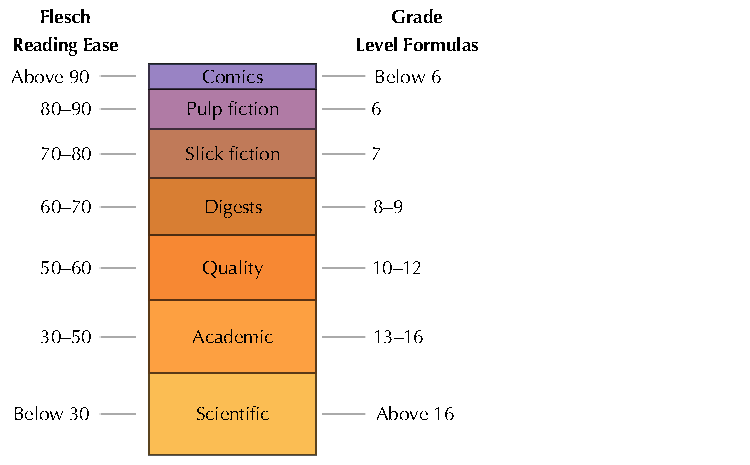
\includegraphics[trim=0cm 0cm 4.5cm 0cm, clip, width=\linewidth]{/Users/erinhengel/Dropbox/Readability/draft/pdf/therm.pdf}
	\end{minipage}
		\floatfoot{\tiny \textit{Notes}. Left-hand-side table displays the formula used to calculate each readability score. Polysyllabic words refers to words with three or more syllables; difficult words are those not found on a list of 3,000 words understood by 80 percent of fourth-grade readers (aged 9--10)~\citep{Chall1995}. The graphic on the right summarises the guidelines for interpreting different readability formulas~\citep{Flesch1962}.}
	}
\end{figure}

The Flesch Reading Ease formula ranks passages of text in ascending order---\emph{i.e.}, more readable passages earn higher scores. The other four formulas generate grade levels estimating the minimum years of schooling necessary to confidently understand an evaluated text---and so more readable passages earn lower scores. To minimise confusion, I multiply the four grade-level scores by negative one. Thus, higher numbers universally correspond to clearer writing throughout this paper.

The constants in each formula vary widely as do the components used to rank vocabulary. Because of these differences, grade-level scores rarely generate identical figures; nevertheless, all five scores produce similar rankings. The yellow box plot in \autoref{figure0X} summarises 165 inter-score correlations found in 25 separate published studies.\footnote{Included in this sample are between-score correlations found in two non-published studies---the present paper (correlations range from 0.53 to 0.97) and  \citet{Benoit2017}.} The median is 0.84.

Readability scores also correlate with alternative measures of text difficulty, including (i) oral reading fluency,\footnote{Generally measured as the number of words read aloud correctly per minute.} (ii) human judgement, (iii) reading comprehension tests and (iv) the cloze procedure.\footnote{The cloze procedure deletes random words in passages of text and ranks their difficulty according to average readers' ability to correctly enter the missing words.} The dark blue box plots in \autoref{figure0X} summarise 166 correlations in 43 published cross-validation studies. Readability scores are highly correlated with reading comprehension and cloze tests; they are also strongly associated with rankings based on human judgement. Correlations with oral reading fluency are more moderate.\footnote{See \aref{appendixmetaanalysis} for a brief overview of the studies included in \autoref{figure0X} and a description of the criteria used to select them.}

\begin{figure}

	\floatbox{figure}[\FBwidth]
	{
		\caption{Meta analysis of correlations with different measures of text comprehension}\label{figure0X}
	}
	{
	\begin{minipage}{0.48\textwidth}
		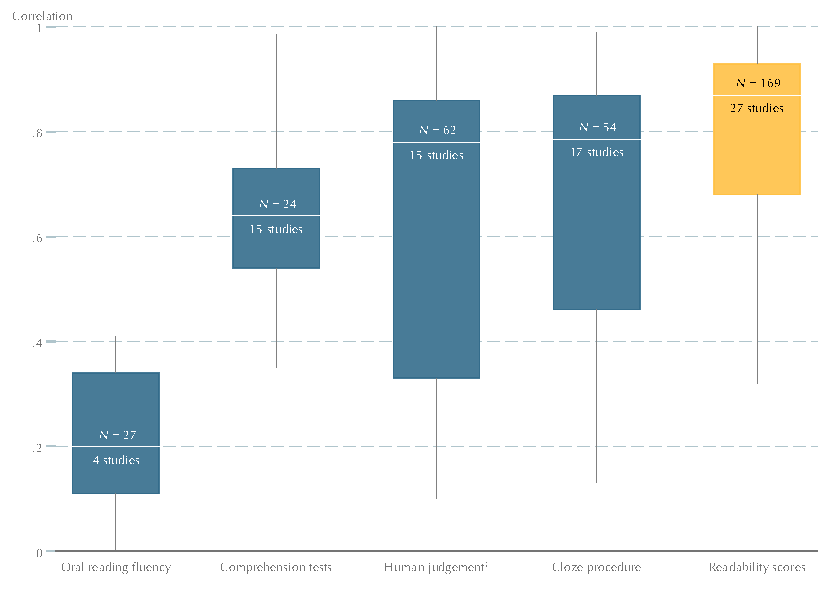
\includegraphics[width=0.95\linewidth]{$HOME/Dropbox/Readability/draft/pdf/figure0X.pdf}
	\end{minipage}
	\begin{minipage}{0.48\textwidth}
		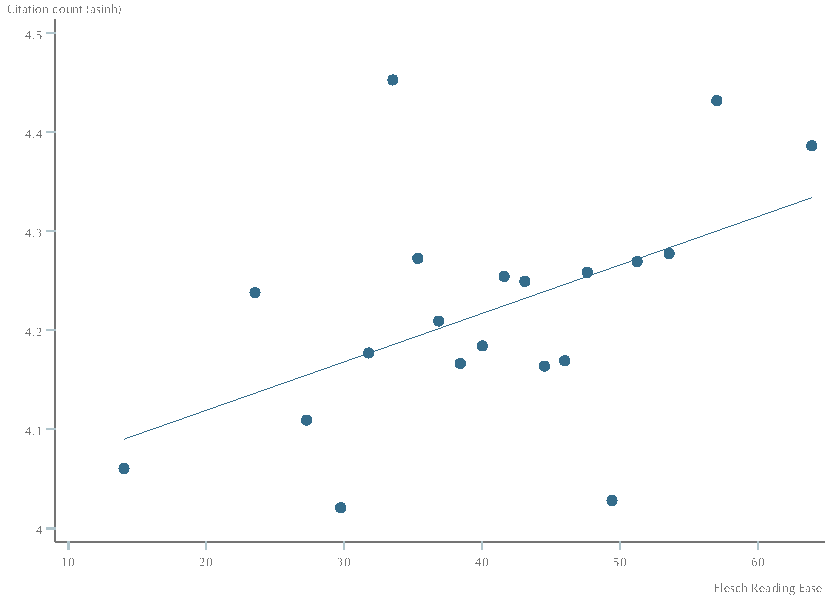
\includegraphics[width=0.95\linewidth]{$HOME/Dropbox/Readability/draft/pdf/asinhCiteCount.pdf}
	\end{minipage}
		\floatfoot{\tiny\textit{Notes}. Graphical display of estimated coefficients of correlation between the five readability scores included in this paper and alternative measures of text comprehension. The figure includes 243 estimates found in 52 separate studies. While I have made every effort to include all relevant studies, the figure is only intended to convey the conclusion that the readability scores used in this analysis are indeed positively correlated with other, arguably more reliable, measures of text difficulty. Please see~\autoref{AppendixMetaAnalysis} for more detailed information of the selection criteria for studies and more detailed information on individual studies.}
	}
\end{figure}

Other studies have validated readability scores against surrogate measures of reading comprehension. More readable high school and college-level correspondence courses have higher completion rates~\citep{Klare1973}. More readable academic journals enjoy larger readership~\citep{Richardson1977,Swanson1948}; their most readable articles win more awards~\citep{Sawyer2008}, are downloaded more often~\citep{Guerini2012}\footnote{In a \href{http://lukaspuettmann.com/2017/12/09/voxeu-gobbledygook/}{blog post}, Lukas Püttmann evaluates the readability of the abstract text of columns published on the \href{http://www.voxeu.org}{VoxEU.org} website and compares them to the number of times that article was viewed. He finds more readable columns are read about 3 percent more often~\citep{Puttmann2017}.} and cited more frequently (see \autoref{figure0X}).\footnote{Evidence linking readability scores and citations in other studies is weaker.  \citet{Lei2016} find a positive yet non-significant relationship between readability in information journals and citations.  \citet{Berninger2017} find a positive correlation between abstract text and citations yet a negative correlation with the text of the actual paper and citations.  \citet{Guerini2012} find that the most readable academic articles are downloaded the most, although their connection to citations is positive, but less important.}

Thanks to high predictive validity and ease of use, readability formulas are widely employed in education, business and government. The U.S. Securities and Exchange Commission encourages clearer financial disclosure forms benchmarked against the Gunning Fog, Flesch-Kincaid and Flesch Reading Ease scores~\citep{Cox2007}. The formulas have also guided readability assessments of, \emph{inter alia}, standardised test questions~\citep{Chall1977,Chall1983}, medical inserts~\citep[\emph{e.g.},][]{Wallace2008}, technical manuals~\citep[\emph{e.g.},][]{Hussin2012,Klare1973}, health pamphlets~\citep[\emph{e.g.},][]{Foster2002,Meade1989} and data security policies~\citep{Alkhurayyif2017}.

In research, readability scores are considered objective proxies for ``complexity''.  \citet{Enke2018} controls for language sophistication using the Flesch Reading Ease formula in a study of moral values in U.S. presidential elections.  \citet{Spirling2016} employs the same score to show that British parliamentarians simplified speeches to appeal to less educated voters in the in the wake of the Great Reform Act.\footnote{\citet{Bischof2018} similarly show a positive link between plain language in political speeches and a desire to appeal to voters using German political manifestos and the Björnsson's readability index. Their study also finds evidence that voters better understand more readable political messages.came to a similar conclusion using German political manifestos and the Björnsson's readability index. Their study also finds evidence that voters better understand more readable political messages.} Legal research has found that judges are more reliant on legislative history when interpreting complex legal statutes, as measured by the Flesch-Kincaid formula~\citep{Law2010}.\footnote{\citet{Long2011} investigate whether a legal brief's readability score correlates with its success on appeal, but find that they do not.} And in finance, various scores have linked the clarity of financial communication materials to better firm and market financial health~\citep{Li2008,Biddle2009,Jansen2011}, larger investment and trading volume ~\citep{Miller2010,Thörnqvist2015,DeFranco2015,Lawrence2013} and lower demand for---albeit higher reliability of---outside research by sell-side analysts~\citep{Lehavy2011}.\footnote{See  \citet{Loughran2016} for a thorough review of the use of readability measures in finance and accounting research.} 

\subsection{Measurement error}
\label{calculation}

Readability scores fail to capture many elements relevant to reading comprehension, including grammar---\emph{e.g.}, active vs. passive tense~\citep{Coleman1964,Coleman1965}---legibility---\emph{e.g.}, typeface and layout---and content---\emph{e.g.}, coherence, organisation and general appeal~\citep{Kintsch1984,Kemper1983,Meyer1982,Armbruster1984}. \footnote{Like intelligence tests, implicit association tests and machine learning algorithms, readability scores are low in causal power.}Nevertheless, ``long sentences generally correspond to complex syntactic structures, infrequent words generally refer to complex concepts, and hard texts will generally lead to harder questions about their content''~\citep[][p. 222,]{Kintsch1984}. Moreover, combining readability scores with measures that capture omitted features does not significantly increase in their predictive power~\citep[see, \emph{e.g.},][]{Kemper1983}.

Readability scores are, however, prone to measurement error. If this error stems from the scores' low causal power and does not partially correlate with the variable of interest (gender), then the analytical results I present in this paper are biased toward zero (classical measurement error). Otherwise, my results will be systematically biased in an unknown direction (non-classical measurement error).

Sources of non-classical measurement error are threefold: (a) grammatical\slash spelling\slash transcription errors in the textual input; (b) bugs in the software that estimates vocabulary complexity and sentence length; or (c) embodied in the jump from using hard words and sentence length to infer readability.

Conditional on accurate calculation, readability scores do combine very precise estimates of vocabulary complexity with almost perfect measures of sentence length. As I argue in \autoref{discussion}, the weighted average of these two variables is informative in much the same way that inferences about readability are. Thus, measurement error related to (c) should only affect the superficial interpretation of observed gender differences. Fundamental conclusions deduced from them should remain intact.

A bigger threat to the identification mapped out in this paper is non-classical measurement error from (a) and (b). I have taken several steps to minimise them. First, I use abstracts---as opposed to the body of a paper---as textual input.\footnote{Prior research has found authors write in a stylistically consistent manner across the abstract, introduction and discussion sections of a paper~\citep{Hartley2003b, Plaven-Sigray2017}.} Abstracts are self-contained, universally summarise the research and are the first and most frequently read part of an article~\citep{King2006}. Moreover, their layout is relatively standardised compared to other parts of a paper: abstracts tend to be surrounded by ample whitespace and most editorial management systems anyway reproduce them in pre-formatted cover pages. These factors suggest a relatively homogenous degree of review across journals and subject matter and limit the impact physical layout and surrounding tables, figures and text have on readability.\footnote{Additionally, all four journals have explicit text layout instructions for submissions; this should further limit the impact layout differences may have had on readability.}

Abstracts are additionally ideal for minimising grammatical\slash spelling\slash transcription errors. They contain few of the features of text which can distort readability scores, \emph{e.g.}, citations, abbreviations and equations. Additionally, most have already (and conveniently) been converted to accurate machine-readable text by digital libraries and bibliographic databases.

A third concern is that some programs that calculate readability scores rely on unclear, inconsistent and possibly inaccurate algorithms to count words and syllables, identify sentence terminations and determine whether a word is on Dale-Chall's easy word list~\citep[for a discussion, see][]{Sirico2007}. Additionally, features of the text---particularly full stops used in abbreviations and decimals in numbers---frequently underestimate average words per sentence and syllables per word.\footnote{Typesetting code used to render equations---common in \emph{Econometrica} abstracts published before 1980---also affects the accuracy of readability scores. I therefore manually replaced all such code with equivalent unicode characters. When no exact replacement existed, characters were chosen that mimicked as much as possible the equation's original intent while maintaining the same character and word counts. Readability scores were determined using the modified text.} To transparently handle these issues and eliminate ambiguity in how the readability scores were calculated, I wrote the Python module \texttt{Textatistic}. Its code and detailed documentation is available at \href{https://github.com/erinhengel/Textatistic}{GitHub}. A brief description is provided in \aref{appendixtextatistic}.

As an additional robustness check, I calculate readability scores using the \texttt{R} \href{https://github.com/trinker/readability}{\texttt{readability} package}. Not only does this alternative software confirm the validity of my own---results are very similar to those reported here---but since the algorithms it uses to calculate the scores is slightly different from my own---\emph{e.g.}, it includes semi-colons among its sentence-ending characters---it suggests the results are robust to minor simplifying changes required when calculating readability scores via computer program instead of manually by a human.\footnote{All five readability scores suggest counting as sentences each grammatically independent unit of thought, not just the groups of words set off by terminal punctuation. Therefore, if a writer uses a semicolon or a dash to connect two independent clauses, that counts as two sentences. Unfortunately, semi-colons are not always used in this manner. They are also used to differentiate items in a list, items which are not, however, independent thoughts. When generating readability scores manually, this is less of an issue---humans can easily determine if a semi-colon is being used in one way or the other. Machines, however, have more difficulty with this task.} 

\section{Data}
\label{abstracts}

\begin{table}
    \footnotesize
    \centering
    \begin{threeparttable}
        \caption{Article count, by journal and decade}
        \label{table1}
        \sisetup{table-figures-decimal=0}
        \begin{tabular}{p{1.5cm}SSSSS}
            \toprule
            {Decade}&{\textit{AER}}&{\textit{ECA}}&{\textit{JPE}}&{\textit{QJE}}&{Total}\\
            \midrule
            1950--59    &            &         120&            &            &         120\\
            1960--69    &            &         343&         184&            &         527\\
            1970--79    &            &         660&         633&           1&        1294\\
            1980--89    &         180&         648&         562&         401&        1791\\
            1990--99    &         476&         443&         478&         409&        1806\\
            2000--09    &         695&         520&         408&         413&        2036\\
            2010--15    &         732&         384&         181&         251&        1548\\
            \midrule
            Total       &        2083&        3118&        2446&        1475&        9122\\
            \bottomrule
        \end{tabular}
        \begin{tablenotes}
            \tiny
            \item \textit{Notes}. Included is every article published between January 1950 and December 2015 for which an English abstract was found (i) on journal websites or websites of third party digital libraries or (ii) printed in the article itself. Papers published in the May issue of \textit{AER} (\textit{Papers \& Proceedings}) are excluded. Final row and column display total article counts by journal and decade, respectively.
        \end{tablenotes}
    \end{threeparttable}
\end{table}

The data include every English article published in \emph{AER}, \emph{Econometrica}, \emph{JPE} and \emph{QJE} between January 1950 and December 2015 (inclusive). The largest sample comes from \emph{Econometrica} which consistently published abstracts with its articles prior to 1950. \emph{JPE} added them in the 1960s and \emph{QJE} in 1980. \emph{AER} came last in 1986.\footnote{Unless otherwise mentioned, observations exclude the May issue of \emph{AER} (\emph{Papers \& Proceedings}).} \autoref{table1} displays data coverage by journal and decade.

The analysis in \autoref{nber} matches published articles with NBER working papers. Matches were first attempted using citation data from RePEc and then by searching NBER's database directly for unmatched papers authored by NBER family members. 1,986 published articles were eventually matched to 1,988 NBER working papers---approximately one-fifth of the data.\footnote{Because a small number of NBER working papers were eventually published as multiple articles or combined into a single paper, the mapping is not one-for-one.} Bibliographic information and abstract text were scraped from \href{http://www.nber.org}{www.nber.org}. See [][NBERStats] for a further description and summary statistics of the data.

The analysis in \autoref{duration} compiles submit-accept times at \emph{Econometrica}---the only journal that makes any kind of disaggregated data on the revision process publicly available.\footnote{Printed at the end of every \emph{Econometrica} article published on or after March 1970 that was not originally presented as an Econometric Society lecture is the date it was first submitted and the date final revisions were received. Before 1970, only ``A Capital Intensive Approach to the Small Sample Properties of Various Simultaneous Equation Estimators'' (January, 1965) included this information. ``Separable Preferences, Strategyproofness, and Decomposability'' (May, 1999) only printed the year of submission; I assume the month is January.} I extracted this information from digitised articles using the open source command utility \texttt{pdftotext}. See \autoref{duration} for summary statistics and a further description.

Controls used in the analysis include, \emph{inter alia} editor fixed effects, institution fixed effects, author productivity fixed effects, English fluency controls, citation counts, and controls for motherhood and childbirth in \autoref{duration}. See \aref{appendixcontrols} for a detailed description of how these controls were generated.

\begin{figure}

	\floatbox{figure}[\FBwidth]
	{
		\caption{Readability by year and \textit{JEL} code}\label{year_jel}
	}
	{
	\begin{minipage}{0.65\textwidth}
		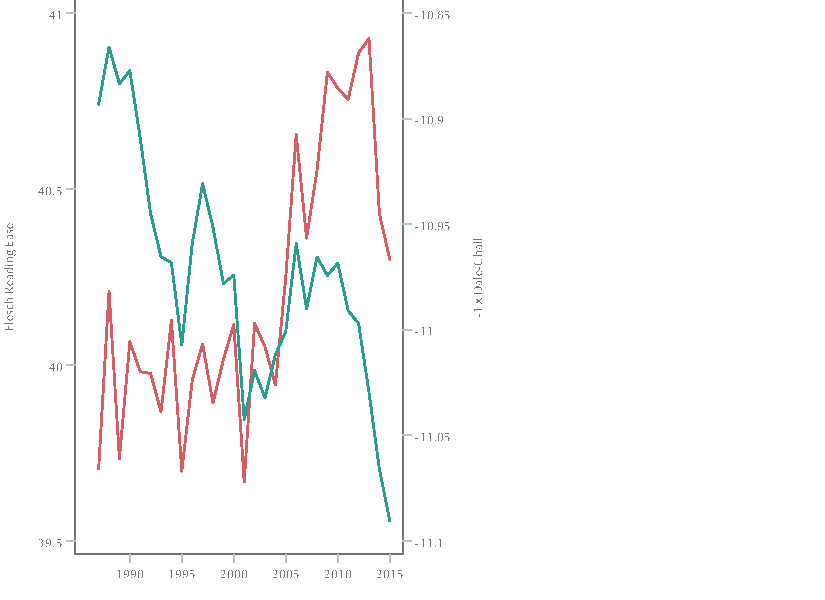
\includegraphics[width=0.95\linewidth]{/Users/erinhengel/Dropbox/Readability/draft/pdf/year.pdf}
	\end{minipage}
	\begin{minipage}{0.3\textwidth}
		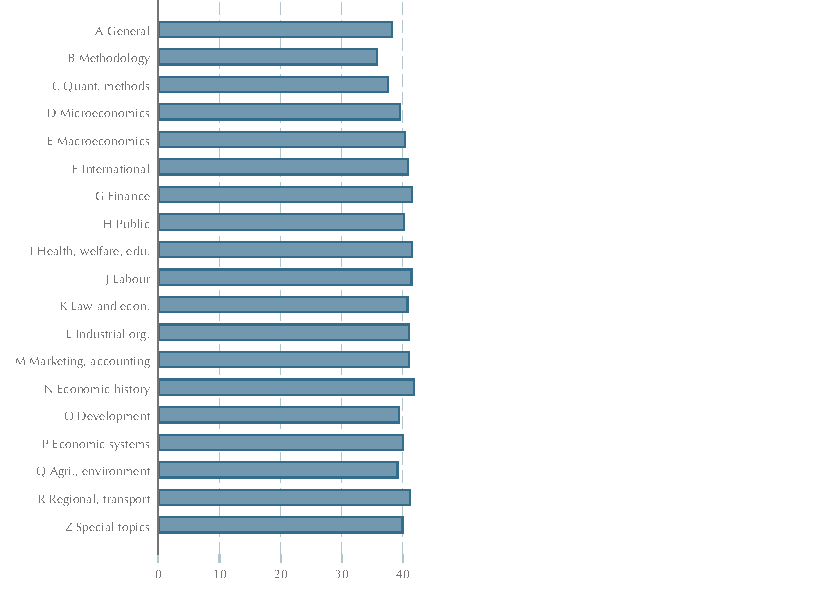
\includegraphics[trim=0cm 0cm 6.95cm 0cm, clip, width=1.1\linewidth]{/Users/erinhengel/Dropbox/Readability/draft/pdf/read_jel.pdf}
	\end{minipage}
		\floatfoot{\tiny\textit{Notes}. Graphical display of estimated coefficients of correlation between the five readability scores included in this paper and alternative measures of text comprehension. The figure includes 243 estimates found in 52 separate studies. While I have made every effort to include all relevant studies, the figure is only intended to convey the conclusion that the readability scores used in this analysis are indeed positively correlated with other, arguably more reliable, measures of text difficulty. Please see~\autoref{AppendixMetaAnalysis} for more detailed information of the selection criteria for studies and more detailed information on individual studies.}
	}
\end{figure}

\subsection{Gender}
\label{data}

Authors were assigned a gender using \href{http://genderchecker.com}{GenderChecker.com}'s database of male and female names. Authors with unisex first names, first names not in the database or those identified only by initial(s) were assigned gender either by me, a research assistant or at least three separate \href{http://www.mturk.com}{Mechanical Turk} workers based on a visual inspection of photos on faculty websites, Wikipedia articles, \emph{etc.} or personal pronouns used in text written about the individual. In situations where the author could not be found but several people with the same first and last name were and all shared the same gender, the author was also assigned that gender. For the remaining cases, I emailed or telephoned colleagues and institutions associated with the author.

Determining the ``gender'' of a paper is not nearly as straightforward. For solo-authored papers---of which there are 3,747 in the sample---gender corresponds to the sex of the author. Unfortunately, top economics journals have collectively published just 269 by women. Only a slightly larger number were written entirely---\emph{or even mostly}---by women (\autoref{figure0}).\footnote{315 papers in the sample were authored entirely by women. Women made up more than 50 percent of all authors in another 47. An additional 35 observations have a female lead authors---\emph{i.e.}, the first author was female in a paper with authors listed non-alphabetically or in which contributions were explicitly noted.} Proportions are similar when the sample is restricted to later years: \emph{QJE} did not publish a single exclusively female-authored paper between 2015--2017 (inclusive); in four of the last fifteen years covered by the data (2001--2015), \emph{Econometrica} and \emph{JPE} didn't either.

\begin{figure}
	\floatbox{figure}[\FBwidth]
	{
		\caption{The representation of women in top economics journals}\label{figure0}
	}
	{
	\begin{minipage}{0.51\textwidth}
		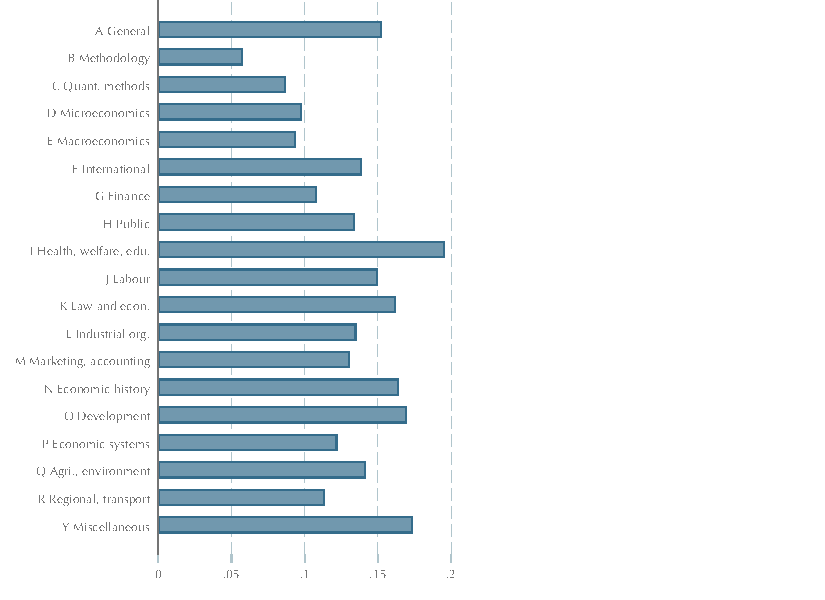
\includegraphics[trim=0cm 0cm 6cm 0cm, clip, width=\linewidth]{/Users/erinhengel/Dropbox/Readability/draft/pdf/jel.pdf}
	\end{minipage}
	\begin{minipage}{0.45\textwidth}
		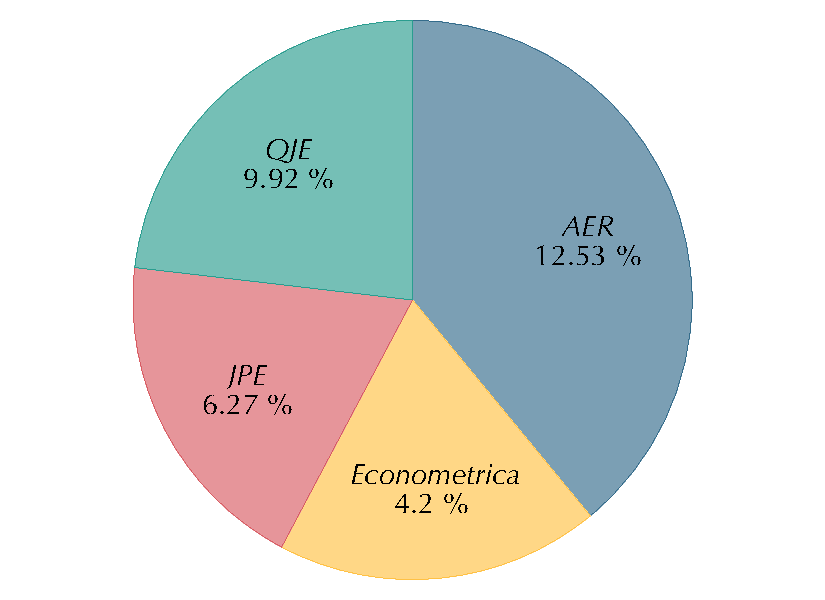
\includegraphics[width=0.95\linewidth]{/Users/erinhengel/Dropbox/Readability/draft/pdf/journal.pdf}
		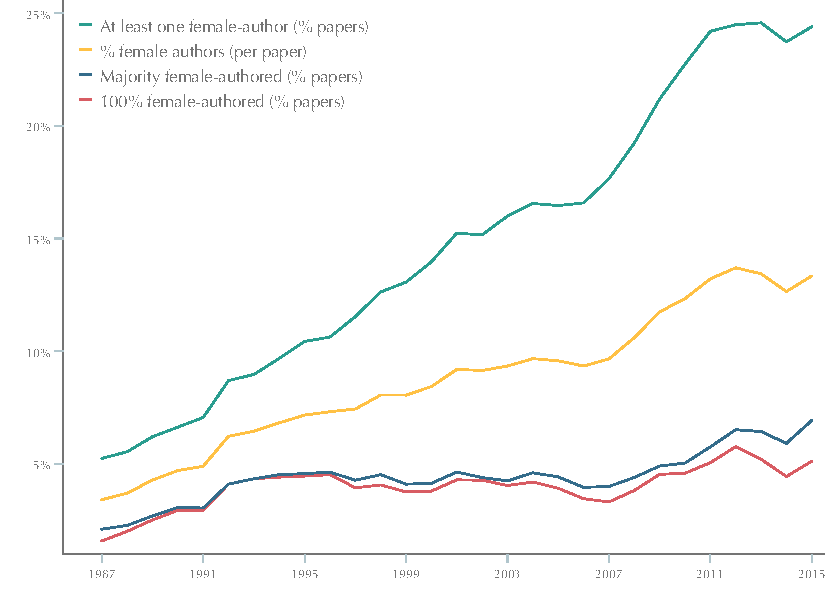
\includegraphics[width=0.95\linewidth]{/Users/erinhengel/Dropbox/Readability/draft/pdf/figure00.pdf}
	\end{minipage}
		\floatfoot{\tiny \textit{Notes}. First graph (upper left-hand corner) shows the percentage of all papers published in top economics journals that authored by more than 50 percent women; second graph (upper right-hand corner) is the percentage of all papers with at least one female author. Third graph (lower left-hand corner) shows the number of so-female-authored papers expressed as a percentage of all solo-authored papers. Final graph (lower right-hand corner) is the average ratio of female authors. See~\autoref{table1} for sample sizes broken down by journal and ten-year increments.}
	}
\end{figure}

A greater number of papers (1,176) are authored by at least one woman. To take advantage of the information contained in this larger sample,  \citet{Blank1991} classified all such papers as ``female''. I opt instead for a less inclusive and continuous measure of gender: the proportion of female authors on a paper.\footnote{This decision was made on the assumption that a gender readability gap---if it exists---is function of (i) the probability a particular portion of analysed text was written and\slash or revised by a female co-author; and (ii) referees' beliefs about female authors' contributions to the writing of a paper. I assume the intersection of (i) and (ii) is positively related to the ratio of female authors on a paper. This assumption is supported by prior research suggesting that co-authors---regardless of seniority---tend to share responsibility for writing and revising collaborative work~\citep{Hart2000,Kumar2016}. [CONFIRM REFERENCE]}

This approach assumes a linear relationship between a paper's readability and its gender composition. (As shown in \autoref{authorlevel}, however, it may be increasing and convex.) As a robustness check, I have repeated most of the analysis (a) on the subset of papers co-authored entirely by a single gender; (b) using a binary variable equal to one if at least one author is female; and (c) using a binary variable equal to one if at least half of all authors are female. Standard errors from (a) tend to be larger; those from (b) and (c) are usually smaller. Result and conclusions are otherwise unchanged (\aref{appendixalternativemeasure}).

\section{Analyses and results}
\label{results}

Analyses and results are organised as follows. In \autoref{articlelevel}, I scrutinise readability at the article level, controlling for editor, journal, year, journal and year interactions, institution, author productivity, article quality, English fluency and field. The results suggest a gap does indeed exist. They also rule out obvious confounding factors---women writing on easier topics, editorial policies in earlier eras, \emph{etc.} Next (\autoref{authorlevel}), I investigate readability at the author-level in a fixed effects regression. This accounts for author-specific productivity, quality and other effects that influence writing---\emph{e.g.}, innate talent---but are otherwise unconnected to peer review.

In \autoref{nber}, I match published articles---which have gone through peer review---to earlier, draft versions of the same papers---which have not. Assuming timing independence, this isolates the effect of peer review and causally links it to the gender readability gap. \autoref{experience} takes the final step and causally links the gap to referees and\slash or editors. I first develop a dynamic model of an author's decision-making process to evaluate the remaining alternatives (\autoref{seumodel}): gender differences in biology\slash behaviour and\slash or knowledge about referee expectations. Based on the model, I propose a method for identifying the impact of discrimination on authors' readability. I then use matching to estimate it (\autoref{seumatching}).

I then document evidence that higher standards affect behaviour and lower productivity. First, prolonged peer review should be one observable repercussion from subjecting female authors to higher standards. Using submit-accept times from \emph{Econometrica}, I evaluate this hypothesis, controlling for, \emph{inter alia}, motherhood, childbirth, citations and field (\autoref{duration}). As a final exercise, I investigate how women react to higher standards as they update beliefs about referees' expectations (\autoref{indirecteffect}).

\subsection{Article-level analysis}
\label{articlelevel}

\autoref{table3} displays each gender's average per sentence number of characters, words, syllables, polysyllabic words and difficult words. Women write shorter, simpler sentences---they contain fewer characters, fewer syllables, fewer words and fewer ``hard'' words. Differences are highly statistically significant.

\autoref{table4} presents coefficients from an ordinary least squares (OLS) regression of the ratio of female co-authors on the five readability scores. To account for error correlation by editorial policy, observations are grouped by journal editor\slash editorial board and standard errors are adjusted accordingly.\footnote{Standard errors are very similar when clustering at the volume-, issue- or paper-level~\citep[see][p. 39--41]{Hengel2016}.}

\begin{table}
    \footnotesize
    \centering
    \begin{threeparttable}
        \caption{Textual characteristics per sentence, by gender}
        \label{table3}
        \begin{tabular}{p{4cm}S@{}S@{}S@{}}
            \toprule
            &{Men}&{Women}&{Difference}\\
            \midrule
            \mrow{4cm}{No. characters}    &      134.72&      130.40&        4.32***\\
                                          &      (0.43)&      (1.45)&      (1.57)   \\
            \mrow{4cm}{No. words}         &       24.16&       23.09&        1.07***\\
                                          &      (0.08)&      (0.26)&      (0.29)   \\
            \mrow{4cm}{No. syllables}     &       40.65&       38.69&        1.96***\\
                                          &      (0.13)&      (0.45)&      (0.48)   \\
            \mrow{4cm}{No. polysyllabic words}&        4.69&        4.31&        0.38***\\
                                          &      (0.02)&      (0.07)&      (0.08)   \\
            \mrow{4cm}{No. difficult words}&        9.38&        8.91&        0.47***\\
                                          &      (0.03)&      (0.12)&      (0.13)   \\
            \bottomrule
        \end{tabular}
        \begin{tablenotes}
            \tiny
            \item \textit{Notes}. Sample 9,122 articles. Figures from an OLS regression of female ratio on each characteristic divided by sentence count. Male effects estimated at a ratio of zero; female effects estimated at a ratio of one. Robust standard errors in parentheses. ***, ** and * difference statistically significant at 1\%, 5\% and 10\%, respectively.
        \end{tablenotes}
    \end{threeparttable}
\end{table}

Column (1) controls for journal and editor: abstracts written only by women score about one point higher on the Flesch Reading Ease scale; according to the four grade-level measures, they take 1--6 fewer months of schooling to understand.\footnote{Coefficients from regressions on Flesch-Kincaid, Gunning Fog, SMOG and Dale-Chall scores represent the marginal effect in years of schooling. Monthly figures found by multiplying each coefficient by 12.} Percentage-wise, women write 1--2 percent better than men.\footnote{Quotient of the coefficient on female ratio divided by the effect for men (ratio of zero) estimated at other co-variates' observed values (see \aref{appendixarticlemale}).}

Column (2) includes 63 year dummies; column (3) adds another 182 journal and year interaction dummies; columns (4) and (5) introduce 64 institution effects, quality controls---citation count and 30 $\text{max. }T_j$ effects (maximum co-author lifetime publication count for paper $j$)---and a dummy variable capturing English fluency.\footnote{In  \citet[][p. 44 and p. 46]{Hengel2016}, I include controls for the order an article appears in an issue---another measure of a paper's quality. Results are similar to those in \autoref{table4}. In addition to the control from English fluency presented here, see \citet[][pp. 35--36]{Hengel2016} for further evicence that the female authors in my data are no more or less likely to be native English speakers.} Coefficients and standard errors in columns (2)--(5) are very similar to those in column (1).

The coefficients on the journal dummies in (2) are presented in \aref{appendixarticlemale}. They compare \emph{AER}'s readability to the readability of \emph{Econometrica}, \emph{JPE} and \emph{QJE}, providing a useful check on the reliability of readability formulas in the context of economic writing. As intuitively expected, all five scores agree that \emph{Econometrica} is harder to read; four out of five scores suggest \emph{JPE} is, too, while \emph{QJE} is easier.

\begin{table}
    \footnotesize
    \centering
    \begin{threeparttable}
        \caption{Gender differences in readability, article-level analysis}
        \label{table4}
        \begin{tabular}{p{2.64cm}S@{}S@{}S@{}S@{}S@{}S@{}S@{}}
            \toprule
            &{(1)}&{(2)}&{(3)}&{(4)}&{(5)}&{(6)}&{(7)}\\
            \midrule
            \mrow{3cm}{Flesch Reading Ease}&        0.88*  &        0.85*  &        0.81   &        0.77   &        0.95*  &        0.50   &        0.87   \\
                                          &      (0.48)   &      (0.48)   &      (0.50)   &      (0.49)   &      (0.50)   &      (0.56)   &      (0.70)   \\
            \mrow{3cm}{Flesch-Kincaid}    &        0.18   &        0.17   &        0.17   &        0.17   &        0.20   &        0.18   &        0.23   \\
                                          &      (0.11)   &      (0.11)   &      (0.11)   &      (0.11)   &      (0.12)   &      (0.13)   &      (0.14)   \\
            \mrow{3cm}{Gunning Fog}       &        0.32** &        0.31** &        0.32** &        0.32** &        0.34** &        0.33** &        0.33** \\
                                          &      (0.12)   &      (0.12)   &      (0.12)   &      (0.13)   &      (0.14)   &      (0.16)   &      (0.16)   \\
            \mrow{3cm}{SMOG}              &        0.20** &        0.20** &        0.20** &        0.20** &        0.22** &        0.19   &        0.21*  \\
                                          &      (0.09)   &      (0.09)   &      (0.09)   &      (0.09)   &      (0.10)   &      (0.12)   &      (0.12)   \\
            \mrow{3cm}{Dale-Chall}        &        0.10** &        0.10** &        0.10** &        0.09** &        0.11** &        0.11*  &        0.13** \\
                                          &      (0.04)   &      (0.04)   &      (0.05)   &      (0.05)   &      (0.05)   &      (0.05)   &      (0.06)   \\
            \midrule
            Editor effects                &           {\ding{51}}   &           {\ding{51}}   &           {\ding{51}}   &           {\ding{51}}   &           {\ding{51}}   &           {\ding{51}}   &           {\ding{51}}   \\
            Journal effects               &           {\ding{51}}   &           {\ding{51}}   &           {\ding{51}}   &           {\ding{51}}   &           {\ding{51}}   &           {\ding{51}}   &           {\ding{51}}   \\
            Year effects                  &               &           {\ding{51}}   &           {\ding{51}}   &           {\ding{51}}   &           {\ding{51}}   &           {\ding{51}}   &           {\ding{51}}   \\
            Journal\(\times\)Year effects          &               &               &           {\ding{51}}   &           {\ding{51}}   &           {\ding{51}}   &           {\ding{51}}   &           {\ding{51}}   \\
            Institution effects           &               &               &               &           {\ding{51}}   &           {\ding{51}}   &           {\ding{51}}   &           {\ding{51}}   \\
            Quality controls              &               &               &               &               &          {\(\text{\ding{51}}^1\)}   &          {\(\text{\ding{51}}^1\)}   &          {\(\text{\ding{51}}^1\)}   \\
            Native speaker                &               &               &               &               &           {\ding{51}}   &           {\ding{51}}   &           {\ding{51}}   \\
            \textit{JEL} (primary) effects&               &               &               &               &               &           {\ding{51}}   &               \\
            \textit{JEL} (tertiary) effects&               &               &               &               &               &               &           {\ding{51}}   \\
            \bottomrule
        \end{tabular}
        \begin{tablenotes}
            \tiny
            \item \textit{Notes}. 9,121 articles in (1)--(5); 5,216 articles in (6); 5,659 articles---including 561 from \textit{AER Papers \& Proceedings} (see~\autoref{footnote34})---in (7). Figures represent the coefficient on female ratio from an OLS regression on the relevant readability score. Quality controls denoted by \(\text{\ding{51}}^1\) include citation count and \(\text{max. }T_j\) fixed effects. Standard errors clustered on editor in parentheses. ***, ** and * statistically significant at 1\%, 5\% and 10\%, respectively.
        \end{tablenotes}
    \end{threeparttable}
\end{table}

Columns (6) and (7) control for primary \emph{JEL} classification. (6) includes 20 fixed effects for primary \emph{JEL} categories; (7) includes 718 effects for tertiary categories. Due to small sample sizes, (7) includes 561 articles from \emph{AER Papers \& Proceedings}.\footnote{\label{footnote34}\emph{AER Papers \& Proceedings} is coded as a separate journal and edited by the American Economic Association's president-elect. \emph{AER Papers \& Proceedings} does not publish abstracts in its print version; only select years and papers are available online (2003 and 2011--2015), all of which are included. Excluding these articles does not impact results or conclusions---coefficients are almost identical to those in column (6), but standard errors are somewhat higher. (Analysis not shown, but is available on request: \href{mailto:erin.hengel@gmail.com}{\texttt{erin.hengel@gmail.com}}.)} Since only post--1990 \emph{JEL} classifications are used, estimates in both columns exclude over 40 percent of the data. Nevertheless, coefficients and standard errors are roughly equivalent, suggesting the readability gap is largely independent of sub-field. \aref{appendixjel} explores this hypothesis in more detail. Conditional on the other explanatory variables, however, there is very little evidence that the gender readability gap is related to sub-fields.

\subsection{Author-level analysis}
\label{authorlevel}

I next analyse readability at the author-level. To disaggregate the data, each article is duplicated $N_j$ times, where $N_j$ is article $j$'s number of co-authors; observation $j_k\in\{1,\ldots,N_j\}$ is assigned article $j$'s $k\text{th}$ author. I then estimate the dynamic panel model in \autoref{equation1}:\begin{equation}\label{equation2}
	R_{jP}=R_{jW}+\beta_{0P}+\beta_{1P}\,\text{female ratio}_j+\bm\uptheta_P\,\vect X_{jP}+\mu_{jP}+\vep_{jP},
\end{equation}$R_{j_{it}}$ is the readability score for article $j$---author $i$'s $t$th publication; $R_{it-1}$ is the corresponding value of author $i$'s $t-1$th paper. Gender enters twice---the binary variable $\text{male}_i$ and $\text{female ratio}_j$---to account for author $i$'s sex and the sex of his co-authors, respectively. $\vect X_j$ is a vector of observable controls. It includes: editor, journal, year, journal $\times$ year, institution and English fluency dummies; quality controls---citation count and $\text{max. }T_j$ fixed effects; and $N_j$ to account for author $i$'s proportional contribution to paper $j$. $\alpha_i$ are author-specific effects and $\vep_{it}$ is an idiosyncratic error. $\alpha_i$ are eliminated by first-differencing; endogeneity in the lagged dependant variable is instrumented with earlier lags~\citep{Arellano1995,Blundell1998}. To account for duplicate articles, the regression is weighted by $1/N_j$.\footnote{Assigning equal weight to all observations results in quantitatively and qualitatively similar results~\citep[see][pp. 44--45]{Hengel2016}.} Standard errors are adjusted for two-way clustering on editor and author.

\begin{table}
    \footnotesize
    \centering
    \begin{threeparttable}
        \caption{Gender differences in readability, author-level analysis}
        \label{table5}
        \begin{tabular}{p{4cm}S@{}S@{}S@{}S@{}S@{}}
            \toprule
            &{\crcell[b]{Flesch\\[-0.1cm]Reading\\[-0.1cm]Ease}}&{\crcell[b]{Flesch-\\[-0.1cm] Kincaid}}&{\crcell[b]{Gunning\\[-0.1cm]Fog}}&{SMOG}&{\crcell[b]{Dale-\\[-0.1cm]Chall}}\\
            \midrule
            \mrow{4cm}{Female ratio (women)}&        2.37** &        0.35*  &        0.66***&        0.47** &        0.23** \\
                                          &      (1.00)   &      (0.20)   &      (0.25)   &      (0.19)   &      (0.10)   \\
            \mrow{4cm}{Female ratio (men)}&        0.58   &        0.10   &        0.15   &        0.09   &        0.10   \\
                                          &      (1.32)   &      (0.25)   &      (0.30)   &      (0.21)   &      (0.11)   \\
            \mrow{4cm}{Female ratio\(\times\)male} &       -1.79   &       -0.26   &       -0.50   &       -0.38   &       -0.14   \\
                                          &      (1.54)   &      (0.32)   &      (0.37)   &      (0.27)   &      (0.13)   \\
            \mrow{4cm}{Lagged score}      &        0.03** &        0.04***&        0.03*  &        0.03*  &        0.03** \\
                                          &      (0.02)   &      (0.01)   &      (0.02)   &      (0.02)   &      (0.01)   \\
            \mcol{\rule{0pt}{4ex}\textit{\(z\)-test for no serial correlation}} \\
            Order 1&      -20.25   &      -15.98   &      -17.14   &      -19.93   &      -20.77   \\
            Order 2                       &        0.55   &       -0.22   &        0.09   &        0.20   &       -0.74   \\
            \midrule
            \(N_j\)              &           {\ding{51}}   &           {\ding{51}}   &           {\ding{51}}   &           {\ding{51}}   &           {\ding{51}}   \\
            Editor effects                &           {\ding{51}}   &           {\ding{51}}   &           {\ding{51}}   &           {\ding{51}}   &           {\ding{51}}   \\
            Journal effects               &           {\ding{51}}   &           {\ding{51}}   &           {\ding{51}}   &           {\ding{51}}   &           {\ding{51}}   \\
            Year effects                  &           {\ding{51}}   &           {\ding{51}}   &           {\ding{51}}   &           {\ding{51}}   &           {\ding{51}}   \\
            Journal\(\times\)Year effects          &           {\ding{51}}   &           {\ding{51}}   &           {\ding{51}}   &           {\ding{51}}   &           {\ding{51}}   \\
            Institution effects           &           {\ding{51}}   &           {\ding{51}}   &           {\ding{51}}   &           {\ding{51}}   &           {\ding{51}}   \\
            Quality controls              &          {\(\text{\ding{51}}^1\)}   &          {\(\text{\ding{51}}^1\)}   &          {\(\text{\ding{51}}^1\)}   &          {\(\text{\ding{51}}^1\)}   &          {\(\text{\ding{51}}^1\)}   \\
            Native speaker                &           {\ding{51}}   &           {\ding{51}}   &           {\ding{51}}   &           {\ding{51}}   &           {\ding{51}}   \\
            \bottomrule
        \end{tabular}
        \begin{tablenotes}
            \tiny
            \item \textit{Notes}. Sample 9,186 observations (2,827 authors). Figures from first-differenced, IV estimation of~\autoref{equation1}~ \citep{Arellano1995,Blundell1998}. Female ratio (women): contemporaneous marginal effect of a paper's female co-author ratio for female authors (\(\beta_1\)); female ratio (men): analogous effect for male authors (\(\beta_1+\beta_2\)). \textit{z}-statistics for first- and second-order autocorrelation in the first-differenced errors~\citep{Arellano1991}; null hypothesis no autocorrelation. Quality controls denoted by \(\text{\ding{51}}^1\) include citation count and \(\text{max. }T_j\) fixed effects. Regressions weighted by \(1/N_j\); standard errors adjusted for two-way clustering on editor and author (in parentheses). ***, ** and * statistically significant at 1\%, 5\% and 10\%, respectively.
        \end{tablenotes}
    \end{threeparttable}
\end{table}

\autoref{table5} displays results. Rows one and two present contemporaneous marginal effects on co-authoring with women for female ($\beta_1$) and male ($\beta_1+\beta_2$) authors, respectively. Both estimates are positive---everyone writes more clearly when collaborating with women. Marginal effects for women are highly significant and at least twice as large as those in \autoref{table4}---women write 2--6 percent better than men.\footnote{Quotient of $\beta_1$ divided by the total effect for men co-authoring with no women (female ratio of zero) estimated at other co-variates' observed values (see \aref{appendixauthormale}).} When men write with women, however, marginal effects are smaller and less precise.

Men and women co-authoring together experience an identical rise (or fall) in readability, so the effect for one should mirror the other. Yet, \autoref{table5} suggests they don't. While the interaction terms ($\beta_2$) are insignificant---\emph{i.e.}, the observed disparity is plausibly due to chance---the difference may reveal an increasing, convex relationship between female ratio and readability. Men's smaller effect potentially reflects their disproportionate tendency to co-author exclusively with other men---precisely where the marginal impact of an additional woman is low.\footnote{On average, the female ratio for men is 0.04 (0.05 excluding solo-authored papers). When excluding articles written entirely by men, their average ratio is still only 0.39. By default, women always author with at least one woman---themselves; the average female ratio of their papers is 0.6 (0.46 and 0.53 excluding articles written entirely by women and solo-authored papers, respectively).}

Tests for serial correlation indicate no model misspecification. Coefficients on the lagged dependant variables are small, suggesting readability is mostly determined contemporaneously. Nevertheless, their uniform positivity and significance indicate modest persistence.

\subsection{Comparing abstracts pre- and post-review.}
\label{nber}

\autoref{table4} establishes a gender readability gap for abstracts published in top economics journals. \autoref{table5} suggests it primarily forms contemporaneously. A possible contemporaneous cause is peer review---specifically referee and\slash or editor demands for more revisions by female authors.

In this section, I show that peer review does indeed cause (or exacerbate) the gender readability gap. To do so, I analyse papers before and after review by comparing published articles to their draft versions. Assuming peer review is the sole gender-related factor to affect abstract readability between versions, a larger increase in women's readability relative to men's is evidence of causality.

\subsubsection{Summary statistics []}
\label{summarystatistics}

As discussed in \autoref{data}, drafts were collected from NBER Technical and Working Paper Series. NBER series were used as the exclusive data source for two reasons. First, approximately one-fifth of articles in the data were originally part of an NBER series, making it the largest single source of draft papers. Second, NBER persistently releases its working papers two to three years before publication (mean 2.1 years)---precisely the length of time spent in peer review~\citep{Ellison2002a,Goldberg2015}.

Does peer review alter abstracts? Prior comparisons of medical journal articles published in the \emph{British Medical Journal} suggest yes---although not a lot.  \citet{Hopewell2014} investigated 93 randomised trials assessing healthcare interventions in human participants published in \emph{BMC}-series medical journals in 2012. A comparison between the original and final submitted manuscript suggested that abstracts were altered in peer review in about 16 percent of all papers, with referees generally asking authors to tone down their conclusions.  \citet{Hayden2008} found no significant change in the Flesch Reading Ease score during peer review itself (submission vs. acceptance), but a significant positive effect from post-acceptance editing by the journal editor and a copy-editor.

Compared to economics journals, however, medical journals ask for fewer revisions~\citep{Ellison2002a,Hayden2008} and enjoy substantially shorter review times~\citep[see, \emph{e.g.},][]{Trauma2015}, suggesting pre-acceptance readability edits are less common. Indeed, as is shown in \autoref{table6}, peer review alters manuscripts by quite a lot.

\autoref{table6} compares textual characteristics between versions. Means in the first three columns are of majority male-authored papers (female ratio strictly below 50 percent); the final three columns are majority female-authored papers (female ratio at or above 50 percent).

\begin{table}
    \footnotesize
    \centering
    \begin{threeparttable}
        \caption{Textual characteristics, published papers vs. drafts}
        \label{table6}
        \sisetup{group-digits=false}
        \begin{tabular}{p{4cm}S@{}S@{}S[round-precision=3]S@{}S@{}S[round-precision=3]}
            \toprule
            &\multicolumn{3}{c}{{Men}}&\multicolumn{3}{c}{{Women}}\\\cmidrule(lr){2-4}\cmidrule(lr){5-7}&{\crcell[b]{Working\\[-0.1cm]paper}}&{\crcell[b]{Published\\[-0.1cm]article}}&{Difference}&{\crcell[b]{Working\\[-0.1cm]paper}}&{\crcell[b]{Published\\[-0.1cm]article}}&{Difference}\\
            \midrule
            \mrow{4cm}{No. sentences}     &        6.47&        5.10&      -1.375***&        6.77&        5.06&      -1.711***\\
                                          &      (0.06)&      (0.04)&     (0.054)   &      (0.15)&      (0.08)&     (0.139)   \\
            \mrow{4cm}{No. characters}    &      862.45&      649.68&    -212.767***&      907.36&      635.97&    -271.385***\\
                                          &      (7.19)&      (4.67)&     (7.160)   &     (18.53)&     (10.31)&    (18.439)   \\
            \mrow{4cm}{No. words}         &      155.70&      115.70&     -40.004***&      164.45&      113.63&     -50.813***\\
                                          &      (1.32)&      (0.85)&     (1.323)   &      (3.42)&      (1.91)&     (3.428)   \\
            \mrow{4cm}{No. syllables}     &      257.01&      193.36&     -63.653***&      269.02&      187.78&     -81.242***\\
                                          &      (2.15)&      (1.40)&     (2.135)   &      (5.54)&      (3.08)&     (5.504)   \\
            \mrow{4cm}{No. polysyllabic words}&       28.36&       21.81&      -6.545***&       28.93&       20.63&      -8.308***\\
                                          &      (0.28)&      (0.18)&     (0.245)   &      (0.71)&      (0.41)&     (0.627)   \\
            \mrow{4cm}{No. difficult words}&       58.51&       44.61&     -13.892***&       60.32&       42.37&     -17.949***\\
                                          &      (0.51)&      (0.33)&     (0.482)   &      (1.30)&      (0.74)&     (1.204)   \\
            \midrule
            \mrow{4cm}{No. words / sentence count}&       24.74&       23.58&      -1.166***&       24.98&       23.16&      -1.820***\\
                                          &      (0.14)&      (0.12)&     (0.124)   &      (0.33)&      (0.27)&     (0.302)   \\
            \mrow{4cm}{No. polysyllabic words / sentence count}&        6.03&        4.45&      -1.576***&        6.05&        4.23&      -1.819***\\
                                          &      (0.07)&      (0.03)&     (0.060)   &      (0.18)&      (0.08)&     (0.155)   \\
            \mrow{4cm}{No. syllables / word count}&        1.66&        1.68&       0.018***&        1.64&        1.66&       0.015***\\
                                          &      (0.00)&      (0.00)&     (0.002)   &      (0.01)&      (0.00)&     (0.004)   \\
            \mrow{4cm}{No. polysyllabic words / word count}&        0.18&        0.19&       0.006***&        0.18&        0.18&       0.005** \\
                                          &      (0.00)&      (0.00)&     (0.001)   &      (0.00)&      (0.00)&     (0.002)   \\
            \mrow{4cm}{No. difficult words / word count}&        0.38&        0.39&       0.009***&        0.37&        0.37&       0.006** \\
                                          &      (0.00)&      (0.00)&     (0.001)   &      (0.00)&      (0.00)&     (0.002)   \\
            \midrule
            \mrow{4cm}{Flesch Reading Ease}&       41.46&       41.13&      -0.332*  &       42.51&       43.08&       0.564   \\
                                          &      (0.26)&      (0.18)&     (0.185)   &      (0.66)&      (0.43)&     (0.452)   \\
            \mrow{4cm}{Flesch-Kincaid}    &      -13.62&      -13.38&       0.243***&      -13.53&      -13.00&       0.531***\\
                                          &      (0.06)&      (0.05)&     (0.050)   &      (0.15)&      (0.11)&     (0.122)   \\
            \mrow{4cm}{Gunning Fog}       &      -17.28&      -17.04&       0.242***&      -17.13&      -16.58&       0.547***\\
                                          &      (0.07)&      (0.05)&     (0.055)   &      (0.18)&      (0.13)&     (0.140)   \\
            \mrow{4cm}{SMOG}              &      -15.14&      -15.00&       0.135***&      -15.02&      -14.70&       0.327***\\
                                          &      (0.05)&      (0.03)&     (0.035)   &      (0.13)&      (0.09)&     (0.095)   \\
            \mrow{4cm}{Dale-Chall}        &      -10.85&      -10.93&      -0.084***&      -10.71&      -10.70&       0.003   \\
                                          &      (0.02)&      (0.02)&     (0.016)   &      (0.06)&      (0.04)&     (0.037)   \\
            \bottomrule
        \end{tabular}
        \begin{tablenotes}
            \tiny
            \item \textit{Notes}. Sample 1,714 published articles authored by more than 50 percent men (1,715 NBER working papers); 272 published articles authored by at least 50 percent women (273 NBER working papers). Figures are means of textual characteristics by sex for NBER working papers and published articles. Third and sixth columns subtract working paper figures (columns 1 and 4) from published article figures (columns 2 and 5) for men and women. Standard errors in parentheses. ***, ** and * difference statistically significant at 1\%, 5\% and 10\%, respectively.
        \end{tablenotes}
    \end{threeparttable}
\end{table}

Abstracts are considerably altered during peer review. \autoref{table6}'s first panel displays raw counts. Draft abstracts are longer---more characters, words and sentences---and denser---more syllables, polysyllabic words and difficult words. The biggest changes are made to female-authored papers: figures in column six are 20--30 percent higher (in absolute value) than those in column three.

Peer review's impact on readability, however, is unclear. Readability scores are weighted averages of the ratios of (i) total word or ``hard'' word to sentence count and (ii) hard word to word count. Between working paper and published versions, (i) decreases and (ii) increases (\autoref{table6}, second panel).\footnote{A greater decline in total word count relative to hard word count may be specific to abstracts, which are edited for length as well as readability. In an analysis of abstracts, introductions and discussions, abstract sentences were shorter but contained more hard words; overall, they had the lowest Flesch Reading Ease scores~\citep{Hartley2003a}.} (i) Peer review shortens sentences and reduces hard words per sentence: in male-authored papers, sentences are 5 percent shorter and contain 26 percent fewer polysyllabic words; in female-authored papers, they are 7 percent shorter and contain 30 percent fewer polysyllabic words. (ii) As a fraction of total word count, however, syllables, polysyllabic words and difficult words rise. To wit, hard word counts and total word count decline, but the latter by proportionately more; their ratios increase: between 1--3 percent for men and 1--2 percent for women.

According to the majority of scores, peer review improves readability (\autoref{table6}, third panel), a finding consistent with similar investigations at medical journals~\citep{Biddle1996,Hayden2008,Roberts1994}.\footnote{\citet{Hayden2008} found no significant change in the Flesch Reading Ease score during peer review itself (submission vs. acceptance), but a significant positive effect from post-acceptance editing by the journal editor and a copy-editor. Compared to economics journals, however, medical journals ask for fewer revisions~\citep{Ellison2002a,Hayden2008} and enjoy substantially shorter review times~\citep[see, \emph{e.g.},][]{Trauma2015}, suggesting pre-acceptance readability edits are less common.} Thanks to fewer hard words per sentence, SMOG scores are higher in published articles regardless of gender (see \autoref{table2}). In female-authored papers, the net effect for remaining scores is similarly positive. In male-authored papers, however, only the Gunning Fog and Flesch-Kincaid scores indicate a positive net effect; for the Flesch Reading Ease and Dale-Chall scores, it's negative. In any case, women's papers endure comparatively greater cuts in hard words relative to total words and larger falls in words per sentence; their abstracts always become more readable during peer review than do those by men.

\begin{figure}
	
	\floatbox{figure}[\FBwidth]
	{
		\caption{Published paper vs. draft readability}\label{figure2}
	}
	{
		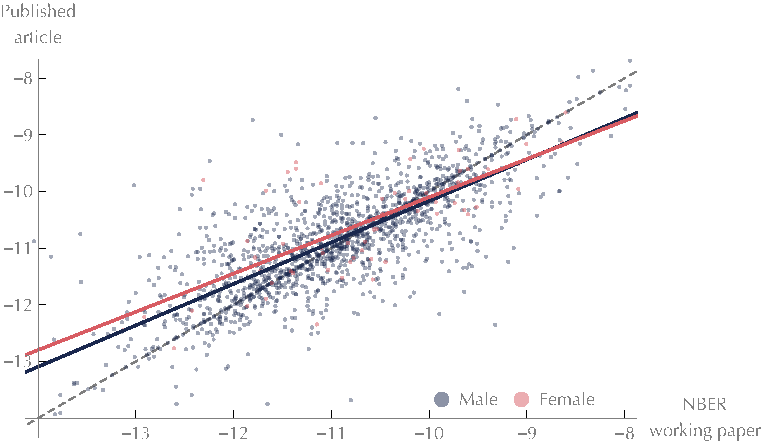
\includegraphics[width=12.3cm]{$HOME/Dropbox/Readability/draft/pdf/figure2.pdf}
		\floatfoot{\tiny \textit{Notes}. Sample 1,631 NBER working papers; 1,629 published articles. Data points represent each abstract's $-1\times\text{Dale-Chall}$ score pre-publicaction (NBER working paper) plotted against its $-1\times\text{Dale-Chall}$ post-publication score. Pink represents women co-authoring only with other women (65 NBER working papers; 64 published articles); blue are men co-authoring only with other men (1,566 NBER working papers; 1,565 published articles); articles co-authored by men and women are omitted. The line of best fit using OLS is shown separately for men and women. The grey dashed line is the 45 degree line through the origin; points above (below) it denote abstracts that were better written after (before) peer review.}
	}
\end{figure}

\autoref{figure2} reiterates women's readability gains. It plots draft Dale-Chall scores ($x$-axis) against abstracts' published scores ($y$ axis) for men (blue) and women (pink). The grey, dashed line is a 45 degree line through the origin. As might be expected, poorly written draft abstracts emerge more readable in the published version (above the 45 degree line); abstracts that were already well written come out slightly less so (below the 45 degree line). Regardless, female-authored published papers are again more readable than they were as working papers relative to male-authored papers---further evidence that women's papers are more heavily scrutinised during peer review.\footnote{An alternative hypothesis consistent with \autoref{figure2} is that male-authored papers are scrutinised more, but edits made as a result reduce readability. The more substantial changes made to female-authored papers documented in \autoref{table6}, however, contradicts this theory.} 

\subsubsection{Identification}
\label{nberidentification}

The data pre- and post-review make it possible to isolate gender differences in readability pre-existing peer review from those incurred during it---and therefore identify gender's contemporaneous effect on peer review scrutiny. The key equation connects published articles to earlier versions of the same paper: scores depend on draft readability as well as factors that affect writing clarity any time \emph{after} being released as working papers. \autoref{equation2} is the OLS representation of this relationship.\begin{equation}\label{equation2}
	R_{jP}=R_{jW}+\beta_{0P}+\beta_{1P}\,\text{female ratio}_j+\bm\uptheta_P\,\vect X_{jP}+\mu_{jP}+\vep_{jP},
\end{equation}where $R_{jP}$ and $R_{jW}$ are readability scores for working ($W$) and published ($P$) versions of paper $j$, respectively. $\beta_{0P}$ is a constant specific to version $P$; $\beta_{1P}$ is the coefficient of interest and reflects the particular impact $\text{female ratio}_j$ has in peer review. $\vect X_{jP}$ and $\mu_{jP}$ are $P$-specific observable (editor, journal, journal-year interactions and English language dummies\footnote{\label{Footnote121}Research may be easier to explain in certain fields. If so, then field affects a published paper's readability because it affects the readability of the underlying working paper and is therefore not due to peer review. By differencing these scores, \autoref{equation2} therefore implicitly already controls for field.} and $\text{max. }t_j$) and unobservable components, respectively.\footnote{\label{Footnote46}$\text{max. }t_j$ is the number of prior papers published in any of the top four economics journals by article $j$`s most prolific co-author. It and the English language dummy are considered $P$-specific because they may influence the degree to which editors and\slash or referees scrutinise the paper. Because all papers in both samples share the same highest-ranked institution (NBER), authors' institutions---which presumably have a similar effect---are omitted.} $\vep_{jP}$ is $P$'s error term.

$P$-specific variables may be correlated with $R_{jW}$. Even if $\mu_{jP}$ and $\text{female ratio}_j$ remain independent, positive correlation between $R_{jW}$ and $\text{female ratio}_j$ (\autoref{table6}) still biases OLS estimates of $\beta_{1P}$ in a direction opposite to the bias on $R_{jW}$. \autoref{equation3} eliminates the distortion by subtracting $R_{jW}$ from both sides of \autoref{equation2}:\begin{equation}\label{equation3}
	R_{jP}-R_{jW}=\,\beta_{0P}+\beta_{1P}\,\text{female ratio}_j+\bm\uptheta_P\,\vect X_{jP}+\mu_{jP}+\vep_{jP}.
\end{equation}Assuming zero partial correlation between $\text{female ratio}_j$ and $\mu_{jP}$, OLS generates an unbiased estimate of $\beta_{1P}$.

An alternative strategy based on \citet{Ashenfelter1994} separately estimates NBER working paper and published article readability using generalised least squares (GLS); $\beta_{1P}$ is identified post-estimation by differencing coefficients. The set-up combines \autoref{equation2} with a relationship defining readability scores \emph{before} external evaluators demand edits (\autoref{equation4}).\begin{equation}\label{equation5}
\mu_{jW}=\gamma+\eta\,\text{female ratio}_j+\bm\updelta_W\,\vect X_{jW}+\bm\updelta_P\,\vect X_{jP}+\omega_j,
\end{equation}where $\beta_{0W}$ is a constant specific to version $W$ and $\beta_{1W}$ reflects $\text{female ratio}_j$'s impact on readability prior to peer review. $\vect X_{jW}$ and $\mu_{jW}$ are version-invariant observable (publication year, citation count, \emph{JEL} effects and $\text{max. }T_j$) and unobservable components, respectively.\footnote{I assume the duration between a paper's NBER release and its publication is too short to influence aggregate time trends; publication year dummies are applied to both working paper and published versions.} $\vep_{jW}$ is version $W$'s error term.

OLS estimates of \autoref{equation4} may be biased by arbitrary correlation between $\mu_{jW}$ and the explanatory variables. \autoref{equation5} defines a general structure for that correlation~\citep{Ashenfelter1994}.\begin{equation}\label{equation5}
\mu_{jW}=\gamma+\eta\,\text{female ratio}_j+\bm\updelta_W\,\vect X_{jW}+\bm\updelta_P\,\vect X_{jP}+\omega_j,
\end{equation}where $\omega_j$ is uncorrelated with $\text{female ratio}_j$, $\vect X_{jW}$ and $\vect X_{jP}$. Substituting \autoref{equation5} into \autoref{equation4} generates the following reduced form representation of $R_{jW}$:\begin{equation}\label{equation7}
	R_{jP}=\,(\wt\beta_{0W}+\beta_{0P})+(\wt\beta_{1W}+\beta_{1P})\,\text{female ratio}_j+\wt{\bm\uptheta}_W\,\vect X_{jW}+\wt{\bm\uptheta}_P\,\vect X_{jP}+\mu_{jP}+\wt\vep_{jP},
\end{equation}where $\wt\beta_{0W}=\beta_{0W}+\gamma$, $\wt\beta_{1W}=\beta_{1W}+\eta$, $\wt{\bm\uptheta}_W=\bm\uptheta_W+\bm\updelta_W$ and $\wt\vep_{jW}=\vep_{jW}+\omega_j$. Similarly, obtain $R_{jP}$'s reduced form by substituting \autoref{equation6} into \autoref{equation2}:\begin{equation}\label{equation7}
	\begin{split}
		R_{jP}=&\,(\wt\beta_{0W}+\beta_{0P})+(\wt\beta_{1W}+\beta_{1P})\,\text{female ratio}_j\\
		&+\wt{\bm\uptheta}_W\,\vect X_{jW}+\wt{\bm\uptheta}_P\,\vect X_{jP}+\mu_{jP}+\wt\vep_{jP},
	\end{split}
\end{equation}where $\wt{\bm\uptheta}_P=\bm\uptheta_P+\bm\updelta_P$ and $\wt\vep_{jP}=\wt\vep_{jW}+\vep_{jP}$. \autoref{equation6} and \autoref{equation7} are explicitly estimated via feasible GLS (FGLS). $\beta_{1P}$ is identifiable post-estimation by subtracting reduced form coefficients; assuming zero partial correlation between $\mu_{jP}$ and $\text{female ratio}_j$, it is unbiased.\footnote{$\mu_{jP}$ may be correlated with $\wt\vep_{jW}$ via $\omega_j$ and\slash or $\vep_{jW}$ without biasing the FGLS estimate of $\beta_{1P}$ because both are uncorrelated with the explanatory variables in \autoref{equation4} (by assumption) and \autoref{equation6} (by definition).}

Both OLS estimation of \autoref{equation3} and FGLS estimation of \autoref{equation6} and \autoref{equation7} require zero partial correlation between $\mu_{jP}$ and $\text{female ratio}_j$ to obtain a valid $\beta_{1P}$.\footnote{Unbiased estimation of $\beta_{1P}$ in \autoref{equation7} requires zero partial correlation between $\mu_{jP}$ and $\text{female ratio}_j$ after controlling for $\vect X_{jW}$ and $\vect X_{jP}$; \autoref{equation3} requires zero partial correlation after controlling for $\vect X_{jP}$, only.} Roughly restated, non-peer review factors must be either independent of its timing (and therefore subsumed in version-invariant fixed effects) or unrelated to gender.\footnote{\label{footnote46}This phrasing is slightly inaccurate but convenient for exposition. Zero correlation between $\text{female ratio}_j$ and $\mu_{jP}$ does not preclude biased estimates of $\beta_{1P}$ when $\mu_{jP}$ is correlated with other explanatory variables that are, in turn, correlated with $\text{female ratio}_j$ by some factor independent of $\mu_{jP}$. Unbiasedness instead requires zero \emph{partial} correlation between $\mu_{jP}$ and $\text{female ratio}_j$.} \autoref{nberresults} evaluates this assumption; briefly, however, I could think of nothing that simultaneously (and convincingly) influences readability, coincides with peer review's timing and correlates with author gender.\footnote{A possible exception is external feedback solicited outside of peer review---\emph{e.g.}, during conferences and seminars. As the next section points out, however, the population of people who provide such feedback overlaps with the population of journal referees. It seems unlikely that this population is biased only in one setting---especially given both settings emphasise gender neutrality.} 

\subsubsection{Results}
\label{nberresults}

\autoref{table7} presents results from OLS estimation of \autoref{equation2}, FGLS estimation of \autoref{equation6} and \autoref{equation7} and OLS estimation of \autoref{equation3}. Since gender bias is possible only when authors' identities are known or can be reasonably guessed, estimates exclude the 279 articles subjected to double-blind review at the \emph{AER} and \emph{QJE} before the internet.\footnote{\label{Footnote51}Excluding these observations does not noticeably impact results or conclusions~\citep[for estimates based on the full sample, see][p. 18]{Hengel2016}.} In the next section, I include these observations and consider their impact.

In order to maximise the sample size, estimates in the first three columns of \autoref{table7} do no include primary \emph{JEL} controls. Estimates including these controls are very similar to those presented in \autoref{table7} and are reproduced in \aref{appendixnberfield}. As discussed in \autoref{Footnote121}, estimates in the final column implicitly control for field, already.

Results in \autoref{table7} strongly indicate the readability gap grew precisely while papers were being reviewed. The first column displays $\beta_{1P}$ from OLS estimation of \autoref{equation2}. According to all five scores, women's readability gains outpace men's between versions. Estimates additionally confirm published readability is correlated with draft readability: coefficients on $R_{jW}$ (shown in \aref{appendixdraftcorr}) are positive and significant---but only about 0.8. A less than unit value suggests $\mu_{jP}$ exerts downward pressure on $R_{jW}$'s coefficient, thereby artificially inflating first column figures (see previous section).

\begin{table}
    \footnotesize
    \centering
    \begin{threeparttable}
        \caption{The impact of peer review on the gender readability gap}
        \label{table7}
        \begin{tabular}{p{4cm}S@{}S@{}S@{}S@{}S@{}}
            \toprule
            &{OLS}&\multicolumn{3}{c}{{FGLS}}&{OLS}\\\cmidrule(lr){2-2}\cmidrule(lr){3-5}\cmidrule(lr){6-6}&{\crcell[b]{Published\\[-0.1cm]article}}&{{\crcell[b]{Working\\[-0.1cm]paper}}}&{\crcell[b]{Published\\[-0.1cm]article}}&{Difference}&{\crcell[b]{Change\\[-0.1cm]in score}}\\
            \midrule
            Flesch Reading Ease           &        1.33** &        2.26** &        3.22***&        0.96*  &        0.94   \\
                                          &      (0.58)   &      (1.01)   &      (1.21)   &      (0.58)   &      (0.59)   \\
            Flesch-Kincaid                &        0.52***&        0.32   &        0.76***&        0.44** &        0.44** \\
                                          &      (0.18)   &      (0.23)   &      (0.28)   &      (0.18)   &      (0.18)   \\
            Gunning Fog                   &        0.52***&        0.44*  &        0.86***&        0.42** &        0.42** \\
                                          &      (0.19)   &      (0.24)   &      (0.29)   &      (0.19)   &      (0.19)   \\
            SMOG                          &        0.30** &        0.33** &        0.56***&        0.24** &        0.24** \\
                                          &      (0.13)   &      (0.16)   &      (0.19)   &      (0.12)   &      (0.12)   \\
            Dale-Chall                    &        0.18***&        0.32***&        0.45***&        0.13** &        0.12** \\
                                          &      (0.05)   &      (0.10)   &      (0.11)   &      (0.05)   &      (0.05)   \\
            \midrule
            Editor effects                &           {\ding{51}}   &           {\ding{51}}   &           {\ding{51}}   &               &           {\ding{51}}   \\
            Journal effects               &           {\ding{51}}   &           {\ding{51}}   &           {\ding{51}}   &               &           {\ding{51}}   \\
            Year effects                  &           {\ding{51}}   &           {\ding{51}}   &           {\ding{51}}   &               &               \\
            Journal\(\times\)Year effects          &           {\ding{51}}   &           {\ding{51}}   &           {\ding{51}}   &               &           {\ding{51}}   \\
            Quality controls              &          {\(\text{\ding{51}}^2\)}   &          {\(\text{\ding{51}}^2\)}   &          {\(\text{\ding{51}}^2\)}   &               &          {\(\text{\ding{51}}^3\)}   \\
            Native speaker                &           {\ding{51}}   &           {\ding{51}}   &           {\ding{51}}   &               &           {\ding{51}}   \\
            \bottomrule
        \end{tabular}
        \begin{tablenotes}
            \tiny
            \item \textit{Notes}. Sample 1,709 NBER working papers; 1,707 published articles. Estimates exclude 279 pre-internet double-blind reviewed articles (see~\autoref{Footnote51}). Column one displays coefficients on female ratio (\(\beta_{1P}\)) from estimating~\autoref{equation2} directly via OLS (see~\aref{appendixdraftcorr} for coefficients on \(R_{jW}\)); standard errors clustered by editor in parentheses. Columns two and three display \(\wt\beta_{1W}\) and \(\wt\beta_{1W}+\beta_{1P}\) from FGLS estimation of~\autoref{equation6} and ~\autoref{equation7}, respectively; standard errors clusterd by year and robust to cross-model correlation in parentheses. Their difference (\(\beta_{1P}\)) is shown in column four. Column five displays \(\beta_{1P}\) from OLS estimation of~\autoref{equation3}; standard errors clustered by year in parentheses. Quality controls denoted by \(\text{\ding{51}}^2\) include citation count, \(\text{max. }T_j\) and \(\text{max. }t_j\); \(\text{\ding{51}}^3\) includes \(\text{max. }t_j\), only (see~\autoref{Footnote46}). ***, ** and * statistically significant at 1\%, 5\% and 10\%, respectively.
        \end{tablenotes}
    \end{threeparttable}
\end{table}

\autoref{table7}'s remaining columns present results from both strategies meant to deal with this bias. Columns 2--4 display FGLS estimates. Coefficients on $\text{female ratio}_j$ from \autoref{equation6} ($\wt\beta_{1W}$) and \autoref{equation7} ($\wt\beta_{1W}+\beta_{1P}$) are shown in columns two and three, respectively. Female-authored working papers and published articles are both better written---but the readability gap is substantially larger in the latter. Flesch-Kincaid, Gunning Fog and SMOG scores imply immediate peer review accounts for 40--60 percent of the total (biased) effect of female ratio in \autoref{equation7}; Flesch Reading Ease and Dale-Chall scores indicate a smaller proportion (30 percent).\footnote{FGLS difference ($\beta_{1P}$, column four) divided by the effect in published articles ($\wt\beta_{1W}+\beta_{1P}$, column three).} Column four displays their difference ($\beta_{1P}$); it is positive and significant for all five scores.

OLS estimates of $\beta_{1P}$ from \autoref{equation3} are shown in \autoref{table7}'s final column. Magnitudes are close to FGLS estimates---confirming earlier conclusions---standard errors are slightly higher. Moreover, given non-bias related factors specific to sub-field that may affect readability in a published paper will similarly affect the readability of a working paper, these estimates already implicitly control for sub-field. Thus, the similarity between the two estimation strategies in \autoref{table7} confirms the findings in \autoref{articlelevel} that, conditional on the other explanatory variables, the gender readability gap is basically independent of field. See \aref{appendixnberfield} for evidence further corroborating this finding.

Both strategies show a significant increase in the gender readability gap \emph{ex post}. Assuming non-peer review factors are always independent of either its timing or gender, this establishes the desired causal link.\footnote{The discussion in \autoref{footnote46} also applies to the precise accuracy of the assumption's phrasing used here.} Threats to this identification strategy are considered next.

\paragraph{Double-blind review before the internet}
\label{doubleblind}

Since gender bias is possible only when authors' identities are known or can be reasonably inferred, estimates in \autoref{table7} exclude the 279 articles in the sample subjected to double-blind review before the internet.\footnote{Forty-three articles with at least one female author and 236 articles with no female author.}

I now consider their impact. Two journals---\emph{QJE} and \emph{AER}---employed double-blind review at some point during the time period covered by the data. \emph{AER}`s spell began 1 July, 1989 and ended 1 July, 2011.\footnote{\label{Footnote66}From 1 May 1987 to 31 May 1989, half of the papers submitted to \emph{AER} were evaluated by single-blind review; the remaining half were subjected to double-blind review~\citep[for details on the trial, see][]{Blank1991}. Referees correctly identified at least one author in 45.6 percent of double-blind reviewed papers---indicating that only about a quarter of the manuscripts were truly double-blind reviewed. I therefore classify every paper published during the trial as having undergone single-bind review. Excluding these observations from the analysis, however, has very little impact; estimated coefficients and standard errors are similar to those presented in \autoref{table8a}.} \emph{QJE} used double-blind procedures until 1 June, 2005. \emph{Econometrica} and \emph{JPE} have never blinded referees to authors' identities.

\autoref{table8a} presents the marginal effect of female ratio by review process based on OLS estimation of \autoref{equation3a}.\begin{equation}\label{equation3a}
	\begin{split}
		R_{jP}-R_{jW}=&\,\beta_{0P}+\beta_{1P}\,\text{female ratio}_j+\beta_{2P}\,\text{Blind}_j+\beta_{3P}\,\text{female ratio}_j\times\text{Blind}_j\\
			&+\bm\uptheta_P\,\vect X_{jP}+\mu_{jP}+\vep_{jP},
	\end{split}
\end{equation}where $\text{Blind}_j$ is a dummy variable equal to 1 if an article was subjected to double-blind review before 1998, the year Google incorporated.\footnote{$\text{Blind}_j$ is equal to 1 for articles published during an official policy of double-blind review. A final publication date, however, may substantially lag the actual review date~\citep[for an illustration and discussion, see][]{Blank1991}. Because results are unchanged when including only \emph{AER} articles published post May 1989 (see \autoref{Footnote66}) and all \emph{QJE} articles published before June 2005 were evaluated under double-blind review, misclassification errors are unlikely to substantially bias estimates presented in \autoref{table8a}.}

Before the internet, double-blind review may have reduced the gender readability gap. \autoref{table8a} suggests a smaller---possibly negative---gap under blinded peer review;\footnote{In a preliminary version of this paper ~\citep{Hengel2015}, I estimated the impact of double-blind review on the gender readability gap in the sample of published papers, only. (It did not compare draft vs. published readability as is done here.) I found that double-blind review was correlated with a higher readability gap. As shown in \aref{appendixdoubleblind}, however, this conclusion is not robust to including time effects.} however, difference-in-difference estimates (reported in the final row) are not statistically significant. Although their consistent direction provides some (weak) evidence that masking authors' identities limits peer review's impact on the gender readability gap, this interpretation should be made with caution given the study did not originally intend to assess the policy's effectiveness.

\begin{table}
    \footnotesize
    \centering
    \begin{threeparttable}
        \caption{The impact of blinded peer review on the gender readability gap}
        \label{table8a}
        \begin{tabular}{p{4cm}S@{}S@{}S@{}S@{}S@{}}
            \toprule
            &{\crcell[b]{Flesch\\[-0.1cm]Reading\\[-0.1cm]Ease}}&{\crcell[b]{Flesch-\\[-0.1cm] Kincaid}}&{\crcell[b]{Gunning\\[-0.1cm]Fog}}&{SMOG}&{\crcell[b]{Dale-\\[-0.1cm]Chall}}\\
            \midrule
            Non-blind                     &        0.93   &        0.43** &        0.41** &        0.23** &        0.13** \\
                                          &      (0.58)   &      (0.18)   &      (0.19)   &      (0.12)   &      (0.05)   \\
            Blind                         &       -1.49   &       -0.56   &       -0.54   &       -0.36   &       -0.13   \\
                                          &      (2.97)   &      (0.68)   &      (0.80)   &      (0.57)   &      (0.17)   \\
            Difference                    &        2.43   &        1.00   &        0.95   &        0.59   &        0.25   \\
                                          &      (3.06)   &      (0.73)   &      (0.84)   &      (0.59)   &      (0.17)   \\
            \midrule
            Editor effects       &           {\ding{51}}   &           {\ding{51}}   &           {\ding{51}}   &           {\ding{51}}   &           {\ding{51}}   \\
            Journal effects               &           {\ding{51}}   &           {\ding{51}}   &           {\ding{51}}   &           {\ding{51}}   &           {\ding{51}}   \\
            Journal\(\times\)Year effects          &           {\ding{51}}   &           {\ding{51}}   &           {\ding{51}}   &           {\ding{51}}   &           {\ding{51}}   \\
            Quality controls              &          {\(\text{\ding{51}}^3\)}   &          {\(\text{\ding{51}}^3\)}   &          {\(\text{\ding{51}}^3\)}   &          {\(\text{\ding{51}}^3\)}   &          {\(\text{\ding{51}}^3\)}   \\
            Native speaker                &           {\ding{51}}   &           {\ding{51}}   &           {\ding{51}}   &           {\ding{51}}   &           {\ding{51}}   \\
            \bottomrule
        \end{tabular}
        \begin{tablenotes}
            \tiny
            \item \textit{Notes}. Sample 1,988 NBER working papers; 1,986 published articles. Columns displays the marginal effect on female ratio for papers undergoing non-blinded review (\(\beta_{1P}\)) and blinded review (\(\beta_{1P}+\beta_{3P}\)) from an OLS estimation of~\autoref{equation3a}. Standard errors clustered by year in parentheses. Quality controls denoted by \(\text{\ding{51}}^3\) includes \(\text{max. }t_j\), only (see~\autoref{Footnote46}). ***, ** and * statistically significant at 1\%, 5\% and 10\%, respectively.
        \end{tablenotes}
    \end{threeparttable}
\end{table}

And in any case, this result does not survive the internet. In \aref{appendixdoubleblind}, I analyse the impact of double-blind review \emph{after} 1998. Gender differences are positive in both single- and double-blind samples, suggesting blinding referees to authors' identities may no longer be the anti-bias fix it possibly once was.\footnote{This conclusion is obviously specific to economics, although it may also apply to fields with an analogous culture of presenting, disseminating and publicising working paper results. Again, please interpret these results with caution.} 

\subsubsection{Robustness}
\label{nberrobustness}

I attribute the difference between NBER abstracts and published abstracts to the peer review process. However, NBER has no word limit while two journals in my sample do: \emph{Econometrica} limits abstracts to 150 words; \emph{AER} limits them to 100 words. It is therefore possible that the effects we observe are due to authors compressing the content of their abstracts rather than due to peer review.

To consider this possibility, I repeat the analysis in \autoref{table7} but this time only on articles whose NBER abstracts fell below the official minimum word limit of the respective journal in which it was published. Results are presented in \aref{appendixwordlimits}. Standard errors are somewhat larger---the subsequent analysis effectively dropped about 40 percent of the observations---but coefficient magnitudes are very similar to those presented in \autoref{table7}, suggesting results in \autoref{table7} are not driven by gender differences in how authors adjust their abstracts to adhere to journals' word limits.

A more serious threat to my identification strategy is violation of timing independence, the principle independence assumption required to causally link the readability gap with peer review. This assumption is violated if male and female authors differ in the changes they make to their manuscripts after releasing them as NBER Working Papers.

Nevertheless, manuscript changes post-submission are probably only made in the context of peer review---either because referees actually request them or authors believe (possibly mistakenly) they will be requested in a future revision.\footnote{This issue of mistaken beliefs is considered in \autoref{experience}.} Thus, timing independence is likely only violated during a narrow window: after a manuscript is released as an NBER Working Paper but before it is submitted to a top-four journal.

\autoref{figure7} suggests that only a small fraction of papers are exposed to this window. It displays a histogram of the length of time between a manuscript's release as an NBER Working Paper and its submission to \emph{Econometrica}. Negative values indicate a manuscript was released as an NBER Working Paper before submission to \emph{Econometrica}---during which timing independence may have been violated. Positive values indicate the manuscript was released as an NBER working paper after submission---suggesting non-peer review factors are indeed independent. Pink represents papers with at least one female author; blue are papers with no female authors.

\begin{figure}
	
	\floatbox{figure}[\FBwidth]
	{
		\caption{Months between NBER release and journal submission}\label{figure7}
	}
	{
		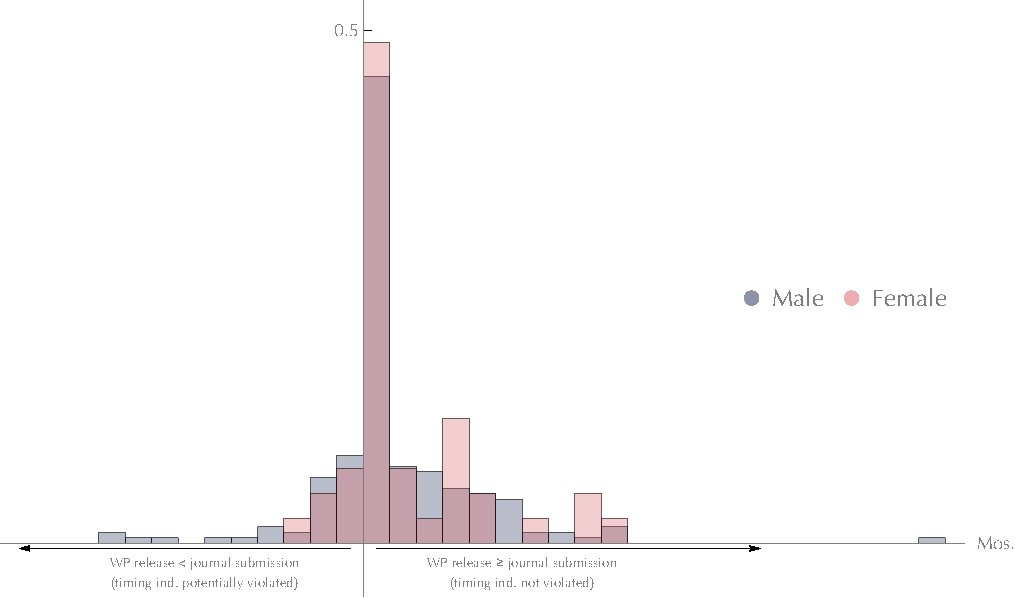
\includegraphics[width=12.3cm]{$HOME/Dropbox/Readability/draft/pdf/figure7.pdf}
		\floatfoot{\tiny \textit{Notes}. Sample 228 articles published in \textit{Econometrica}. Figure represents the distribution of the difference (in months) between a paper's release as an NBER Working Paper and submission of that same article to \textit{Econometrica} (where it is eventually published). To the right-hand side of the \(y\)-axis are articles that were released as working papers \textit{after} they they had already been submitted to \textit{Econometrica}. To the left of the \(y\)-axis are articles that were released \textit{first} as an NBER Working Paper and submitted to \textit{Econometrica} at a later date.}
	}
\end{figure}

Most manuscripts published in \emph{Econometrica} are submitted to peer review at the same time or before they are released as NBER Working Papers. This is particularly true for female-authored papers---only 15 percent are released as working papers first.\footnote{The corresponding figure for male-authored papers is 21 percent. The conclusion that more female-authored papers are submitted to peer review before submission to \emph{Econometrica} is robust to controlling for year fixed effects (see \aref{appendixdoubleblind}).} Assuming similar submission-release patterns in \emph{AER}, \emph{JPE} and \emph{QJE}, \autoref{figure7} suggests that violation of timing independence is only an issue in a small number of predominately male authored papers.\footnote{This possibly biases estimates in \autoref{table7} downward.}

Moreover, a textual analysis of the acknowledgements sections suggests that most NBER Working Papers have been widely circulated among colleagues and presented at seminars and conferences prior to their release. The average length of an acknowledgement section in an NBER Working Paper is 133 words. Most thank at least one person for helpful comments (and the vast majority thank several) and almost all were presented in at least one conference prior to release.

This evidence combined with the evidence presented in \autoref{figure7} suggests that even if male and female authors differ in how likely they are to send working papers out for comments, who they send those papers to and how they respond to those comments, gender differences in this respect occur \emph{before} a paper is released as a working paper---and any changes in readability that occur between the NBER Working Paper and the published paper are indeed due to the refereeing process.

The only remaining external factor I am aware of that might confound this assumption is the feedback women receive in conferences and seminars. Perhaps women tighten prose (before or after submission) in response to audience member remarks? Anecdotal evidence suggests female speakers are given a harder time,\footnote{A related theory is that women receive more critical feedback in conferences and seminars because they present their work more often. In a survey of economists,  \citet{Sarsons2015} finds that men and women are equally likely to present co-authored work but women are actually \emph{less} likely to present solo-authored work.} although I could find no scientific analysis to support (or contradict) this claim.\footnote{A recent \href{https://chroniclevitae.com/news/1182-should-academic-conferences-have-codes-of-conduct}{article} on Chronicle Vitae discusses the topic and provides specific examples~\citep{Baker2015}. SXSW Interactive (a large technology conference that isn't specifically linked to academia) cancelled two 2015 panel discussions on issues related to gender in response to violent online harassment of the (female) speakers.} Nevertheless, most participants are also current (or future) journal referees. Neutral review feedback is inconsistent with non-neutral presentation feedback when originating from the same group.\footnote{Even if this were the case, it implies an entrenched discipline-wide bias.} 

\subsection{Investigating readability over authors' lifetimes}
\label{experience}

The wider gap post-peer review confirms a causal link with peer review. It does not assure causality with referee scrutiny. In this section, I evaluate the alternatives: women write more clearly because of gender differences in (i) biology\slash behaviour---\emph{e.g.}, they're more sensitive to referee criticism---or (ii) knowledge about referee expectations---\emph{e.g.}, by overestimating the importance of writing well.

In a dynamic model of authors' decision-making processes, I show that any gap caused exclusively by (i) or (ii) declines with experience. Yet the gap does not decline. It widens. Estimates from pooled subsamples and matching indicate women write more clearly as their publication count increases; men, possibly less so. This pattern of behaviour suggests discrimination---either directly in the form of biased referee scrutiny or indirectly from biased referee assignment (\autoref{Theorem1}).

\subsubsection{Theoretical framework}
\label{seumodel}

To organise the analysis, I develop a simple dynamic model of readability's marginal impact on an author's decision making process. It follows an author---denoted by $i$---who publishes several articles in prestigious academic journals over the course of his career. Each article is roughly equivalent in terms of topic, novelty and quality, but varies on readability.

At stage 0, author $i$ drafts his $t$th paper and submits it for peer review. Upon receipt, the journal's editorial office assigns the manuscript to a group of referees. The (finite) set of all potential review groups is represented by $\Sigma$; $\mu_i$ is the set of strictly positive probability measures on $\Sigma$. $\Sigma$ and $\mu_i$ are known to $i$.

Let $r_{0it}$ and $\widetilde r_{0i}^s$ denote manuscript $t$'s non-negative draft readability and the initial rejection threshold review group $s\in\Sigma$ applies to all papers by author $i$, respectively. $s$ rejects the paper at stage 0 if $$r_{0it}<\widetilde r_{0i}^s.$$ $i$ is otherwise granted a ``revise and resubmit'' (R\&R), yet could still be rejected at stage 1 if the readability of his revised manuscript, $R_{it}=r_{0it}+r_{1it}$, does not meet a second threshold, $$R_{it}<\widetilde R_i^s,$$ where $\widetilde R_i^s=\widetilde r_{0i}^s+\widetilde r_{1i}^s$. All rejections and acceptances are final. $\widetilde R_i^s\ne\widetilde r_{0i}^s$ to account for different standards at different stages of peer review. $r_{1it}$, $\widetilde r_{0i}^s$ and $\widetilde r_{1i}^s$ are non-negative; the latter two are independent.

To aid the revision process, $s$ writes a referee report from which $i$ forms expectations about $\widetilde R_i^s$ by assigning subjective probabilities $\pi_{1it}^s(R)$ to all $R$. Unfortunately, the concept of readability is complex, some referees write insufficiently detailed reports and inattentive or hypersensitive authors misconstrue even perfectly clear advice. This renders $i$'s interpretation of the report imprecise and his subsequent expectations about $\widetilde R_i^s$ inexact and possibly specious.

Conditional on $r_{0it}$, I assume referee reports by $s$ for $i$ are the same for all $t$ and that each is distinctive enough for $i$ to distinguish $s$ in $\Sigma$.\footnote{Should $s$ review a future paper by $i$, $i$ would recognise it as the same (anonymous) group that reviewed his earlier paper. This does not imply that the report reveals individual referees' identities.} Consequently, author $i$'s stage 1 choice of $R_{it}$ maximises his (immediate) subjective expected utility given $s$,\begin{equation}\label{cost}
	c_m(\hat x_m)=c_f(\hat x_f),
\end{equation}$\Pi_{1it}^s(R_{it})$ is the cumulative sum of $\pi_{1it}^s(R)$ for all $R\le R_{it}$; $u_i$ is the utility of having a paper accepted in a prestigious journal;\footnote{Authors probably care about getting their papers accepted and they may care about writing well, but their marginal utility from the intersection of the two events---\emph{i.e.}, higher utility from writing well \emph{only} because the paper is published in a top-four journal (as opposed to a top field journal or second-tier general interest journal)---is assumed to be negligible.} $\phi_{i|r_{0it}}(r_{1it})=\phi_i(R_{it})-\phi_i(r_{0it})$ and $c_{i|r_{0it}}(r_{1it})=c_{i}(R_{it})-c_{i}(r_{0it})$ are the satisfaction and cost, respectively, from making changes $r_{1it}$ given the paper's initial readability $r_{0it}$. $\phi_i$ is increasing and concave in its arguments, $c_i$ increasing and convex---marginally higher $R_{it}$ generates proportionally less satisfaction but needs more effort when the paper is already well written. $c_i(0)$ and $\phi_i(0)$ are 0.

Authors' decisions at stage 0 are myopic; $i$'s choice of $r_{0it}$ maximises his initial subjective expected utility for the current paper,\begin{equation}\label{equation16}
\begin{split}
	\text{revision duration}_j = 	&\, \beta_0+\beta_1\,\text{female ratio}_j +\beta_2\,\text{mother}_j + \beta_3\,\text{birth}_j \\
									& + \beta_4\,\max~t_j + \beta_5\,\text{no. pages}_j + \beta_6\,N_j + \beta_7\,\text{order}_j \\
									& + \beta_8\,\text{citations}_j + \beta_9\,\text{flesch}_j + \beta_{10}\,\text{theory}_j + \beta_{11}\,\text{empirical}_j\\
									& + \beta_{12}\,\text{other}_j + \bm\uptheta\,\vect X_j + \vep_j,
\end{split}
\end{equation}where $\Pi_{0it}^s(r_{0it})$ is the cumulative sum for all $r\le r_{0it}$ of author $i$'s subjective probabilities $\pi_{0it}^s(r)$ about $\widetilde r_{0i}^s$; $v_{1it}^s$ is \autoref{equation8} evaluated at the optimal $r_{1it}$.

Authors update subjective probabilities (i) using relevant information from their own experience in peer review; and (ii) by observing others' readability choices and publication outcomes. When evidence from (i) contradicts evidence from (ii), (i) takes precedence. These assumptions imply, at a minimum, that $i$ updates $\Pi_{0it}^s$ and $\Pi_{1it}^s$ based on conclusive evidence derived from the choices and outcomes of equivalent peers (\autoref{Definition1})\footnote{\label{Footnote64}Specifically, if $i$ observes with probability 1 that in state $s$ an equivalent author $k$ receives an R\&R at $r_{0k}$, then $\Pi_{0it}^s(r)=1$ for all $r\ge r_{0k}$. Similarly, if $i$ observes with probability 1 that in state $s$, $k$ is accepted at $R_k$, then $\Pi_{1it}^s(R)=1$ for all $R\ge R_k$.} and knowledge acquired during his own prior experience in peer review.\footnote{\label{Footnote70}If $i$ is accepted at stage 1 in time $t'$ for review group $s$, then $\Pi_{1it}^s(R)=1$ for all $t>t'$ and $R\ge R_{it'}$; otherwise, $\Pi_{1it}^s(R)=0$ for all $t>t'$ and $R\le R_{it'}$. Similarly, if $i$ receives an R\&R at stage 0 in time $t'$ for review group $s$, then $\Pi_{0it}^s(r)=1$ for all $t>t'$ and $r\ge r_{0it'}$; otherwise, $\Pi_{it}^s(r)\,\le\Pi_{it'}^s(r)$ for all $t>t'$, $r\le r_{0it'}$ and $s\in\Sigma$.}

\begin{definition}\label{Definition1}
	Equivalent authors write identical papers in terms of topic, novelty and quality.
\end{definition}



\autoref{equation8} and \autoref{equation9} incorporate a variety of factors that potentially affect authors' readability choices---editorial standards ($\widetilde r_{0i}^s$ and $\widetilde R_i^s$); ambition ($u_i$); the cost of drafting and revising manuscripts ($c_i$); an otherwise unexplained intrinsic satisfaction from writing readable papers ($\phi_i$). Poor information, overconfidence and sensitivity to criticism are not explicitly included, on the assumption that people do not \emph{want} to be poorly informed, overconfident or excessively sensitive. These factors nevertheless enter \autoref{equation8} and \autoref{equation9}---and hence influence choices---via the subjective expectations authors form about $\widetilde r_{0i}^s$ and $\widetilde R_i^s$.

A single $R_{it}$ cannot, therefore, establish if and to what extent $i$'s choices are motivated by (a) preferences and costs specific to him ($u_i$, $\phi_i$, $c_i$), (b) editorial standards and\slash or referee assignment outside his control ($\widetilde r_{0i}^s$, $\widetilde R_i^s$, $\mu_i$) or (c) miscellaneous confounding factors mopped by $\Pi_{0it}^s$ and $\Pi_{1it}^s$. Since preferences and costs are time independent, however, an observed increase in $i$'s choice of readability at two separate $t$ distinguishes (a) from the combined impact of (b) and (c).\footnote{The analysis in \autoref{nber} similarly establishes that (b) and\slash or (c) are significant factors driving the choice of $R_{it}$. It cannot, however, distinguish \emph{between} (b) and (c).} $i$ may be more sensitive to criticism and he might prefer writing more clearly; nevertheless, he improves readability today relative to yesterday only when he believes it boosts his chances of publishing.

Moreover, because (c) does not reflect activities or states the author enjoys, its impact on choices declines with experience. Authors may miscalculate referee expectations and misconstrue their reports, but with experience they correct their mistakes. Having ruled out (a) and holding acceptance rates constant, this implies that a persistent readability gap between equivalent peers is caused by (b)---\emph{i.e.}, editorial standards and\slash or referee assignment beyond authors' control.

I capture this idea in \autoref{Theorem1}, where $\bm1_{0i}^s(r)$ and $\bm1_{1i}^s(R)$ are indicator functions equal to 1 if $r\ge\widetilde r_{0i}^s$ and $R\ge\widetilde R_i^s$, respectively, and $\Sigma_{A_{it}}$ is the collection of $s\in\Sigma$ for which $\bm1_{0i}^s(r_{0it})\bm1_{1i}^s(R_{it})=1$. \autoref{Theorem1} is proved in \aref{appendixproofs}.

\begin{theorem}\label{Theorem1}
	Consider two equivalent authors, $i$ and $k$, that satisfy the following three conditions.
	\begin{enumerate}[label=Condition \arabic*., leftmargin=*, widest*=2]
		\item $(r_{0kt},R_{kt})\le(r_{0it},R_{it})$ for all $s\in\Sigma_{A_{it}}$ and $t>t'$ and there exists $K'>0$ such that for at least one $s\in\Sigma_{A_{it}}$ and no $t>t'$, $||(r_{0it},R_{it})-(r_{0kt},R_{kt})||<K'$.
		\item For at least one $t''<t'$, $(r_{0it''},R_{it''})<(r_{0it'},R_{it'})$ and there exists $K''>0$ such that for no $t>t'$, $||(r_{0it},R_{it})-(r_{0it''},R_{it''})||<K''$.
		\item $\int_\Sigma\!\bm1_{0i}^s(r_{0it})\bm1_{1i}^s(R_{it})\,\dd\mu_i\le \int_\Sigma\!\bm1_{0k}^s(r_{0kt})\bm1_{1k}^s(R_{kt})\,\dd\mu_k$ for all $t>t'$.
	\end{enumerate}
Then, almost surely, referee assignment is biased in favour of $k$, $$\int_\Sigma\!\bm1_{0i}^s(r_{0kt})\bm1_{1i}^s(R_{kt})\,\dd\mu_i<\int_\Sigma\!\bm1_{0i}^s(r_{0kt})\bm1_{1i}^s(R_{kt})\,\dd\mu_k,$$ or referee scrutiny is biased against $i$, $$\int_\Sigma\!\bm1_{0i}^s(r_{0kt})\bm1_{1i}^s(R_{kt})\,\dd\mu_i<\int_\Sigma\!\bm1_{0k}^s(r_{0kt})\bm1_{1k}^s(R_{kt})\,\dd\mu_i,$$
or both.
\end{theorem}

\autoref{Theorem1}`s three conditions are sufficient to verify discrimination in academic publishing: when female authors' unconditional probability of acceptance is no higher than men's (Condition 3), their current papers are more readable than their past papers (Condition 2) and also \emph{persistently} more readable than men's papers (Condition 1) then either editors assign women ``tougher'' referees---\emph{i.e.}, those with higher $\widetilde r_{0i}^s$ and\slash or $\widetilde R_i^s$---or referees apply higher standards to women's writing---\emph{i.e.}, $\widetilde r_{0k}^s<\widetilde r_{0i}^s$ and\slash or $\widetilde R_k^s<\widetilde R_i^s$ for at least one $s\in\Sigma$.

\paragraph{Measuring discrimination}
\label{matchingidentificaiton}

\autoref{Theorem1}'s three conditions confirm the presence of discrimination. They principally rely on two identifying assumptions: (i) $i$ and $k$ are equivalent; (ii) $t'$ is sufficiently large---\emph{i.e.}, any errors in $i$'s beliefs about $\widetilde r_{0i}$ and $\widetilde R_i$ are on a path converging to zero. By assuming a more specific belief structure at $t'$, \autoref{Corollary1} proposes a conservative measure of discrimination's impact on readability choices.

When making revisions, authors choose $R_{it}$ to maximise \autoref{equation8}. As shown in \aref{appendixproofs}, $R_i^\star\le r_{0it}$ where $R_i^\star$ is the $R$ that solves $\phi_i'(R)=c_i'(R)$. Since $R_i^\star$ is $i$'s optimal readability in the absence of peer review and $R_i^\star\le r_{0it}$, $i$ prefers $R_{it}>r_{0it}$ only if $r_{0it}<\widetilde R_i^s + e_{1it}^s$, where $e_{1it}^s$ is his time $t$ error in beliefs about $\widetilde R_i^s$. So $i$ revises only when required---and even then, no more than a comfortable minimum to placate referees.

A similar logic governs $i$'s choice of $r_{0it}$---now picked to maximise \autoref{equation9}. $i$ opts for $r_{0it}>R_i^\star$ only if $R_i^\star<\widetilde r_{0i}^s+e_{0it}^s$ for at least one $s$ in $\Sigma_{A_{it}}$, where $e_{0it}^s$ is the time $t$ error in $i$'s beliefs about $\widetilde r_{0i}^s$. Thus\begin{equation}\label{equation10}
	 r_{0it}=\max\left\{R_i^\star,\widetilde r_{0i}^{\overline s}+e_{0it}^{\overline s}\right\}\quad\text{and}\quad R_{it} = \max\left\{r_{0it},\widetilde R_i^s+e_{1it}^s\right\},
\end{equation}
where $\overline s$ is the review group in $\Sigma_{A_{it}}$ for which $i$ believes $\widetilde r_{0i}^s$ is highest---\emph{i.e.}, $\overline s\in\Sigma_{A_{it}}$ satisfies $\widetilde r_{0i}^s+e_{0it}^s\le\widetilde r_{0i}^{\overline s}+e_{0it}^{\overline s}$ for all $s\in\Sigma_{A_{it}}$.\footnote{\label{Footnote68}As shown in \autoref{Theorem1}'s proof (\aref{appendixproofs}), $i$'s beliefs about $\widetilde r_{0i}^s$ and $\widetilde R_i^s$ converge from above. Coupled with Jensen's inequality, this means $\widetilde r_{0i}^s+e_{0it}$ and $\widetilde R_i^s+e_{1it}^s$ may exceed $i$'s time $t$ expectations of $\widetilde r_{0i}^s$ and $\widetilde R_i^s$, respectively. At the limit, however, $e_{0it}^s$ and $e_{1it}^s$ converge to 0---so as $t$ increases, this ``comfort buffer'' declines.}

Define $\delta_{0ik}^s$ and $\delta_{1ik}^s$ as the difference in readability standards applied to authors $i$ and $k$ by review group $s$ in time $t$ at stage 0 and 1, respectively: $$\delta_{0ik}^s\equiv\widetilde r_{0i}^s-\widetilde r_{0k}^s\quad\text{and}\quad\delta_{1ik}^s\equiv\widetilde R_i^s-\widetilde R_k^s.$$ When $\delta_{0ik}^s\ne0$ and\slash or $\delta_{1ik}^s\ne0$, $s$ employs asymmetric evaluation criteria to $i$ and $k$'s work.\footnote{The asymmetry's direction is captured in the sign: positive if $s$ is tougher on $i$; negative otherwise.} Dissimilar authors may call for asymmetric benchmarks---but if $i$ and $k$ are equivalent, they're a form of discrimination. Unfortunately, $\widetilde r_{0i}^s$ and $\widetilde R_i^s$ are not known to the researcher and $R_{it}$ inconsistently estimates them (\autoref{equation10}). As \autoref{Corollary1} shows, however, $R_{it}-R_{kt}$ is \emph{smaller} in magnitude than the true value of stage 1 discrimination by $s$ or stage 0 discrimination by $\overline s$.

\begin{corollary}\label{Corollary1}
	Let $i$ satisfy the assumptions and conditions of \autoref{Theorem1} relative to $k$ and assume that for all $t\ge t'$:
	\begin{enumerate}[label=Assumption \arabic*., leftmargin=*, widest*=2, start=4]
		\item $e_{it}=e_{kt}$.
		\item $e_{it}$ and $e_{kt}$ are on a path converging to zero.
	\end{enumerate}
	Then~\autoref{eq:correq1} is a conservative estimate of the impact higher standards play in $i$'s time $t'$ readability choice:
	\begin{equation}
		D_{ik}\equiv R_{it'}-\max\left\{R_{it''},R_{kt'}\right\},
		\label{eq:correq1}
	\end{equation}
	where $R_{it''}$ is the readability of $i$'s time $t''<t'$ paper, as defined in~\autoref{Theorem1}, Condition 2.
\end{corollary}

\autoref{Corollary1} identifies a conservative measure of discrimination's impact on $i$'s readability. It also exposes the toxic denouement of one biased $s$. $i$'s time $t$ readability choice depends on discrimination at stage 1 by the group of referees that actually reviewed his paper ($s$) as well as discrimination at stage 0 by another review group that (probably) didn't ($\overline s$).

Such is the first externality from even one rotten apple. From $i$'s perspective, $\overline s$ spoils the bunch. Bias from $\overline s$ destabilises $s$'s attempt to treat $i$ and $k$ fairly. Either $i$ is rejected when assigned to $\overline s$ or discrimination by $\overline s$ affects $i$'s readability even when $i$ is reviewed by referees who do not discriminate.

Moreover, offsetting unfairness with fairness only works when \emph{everyone} is fair. Asymmetry from one upsets symmetric criteria applied everywhere else, creating endless imbalance when some people just will not be fair. If culture and\slash or behaviour predicate bias against $i$ and restrain comparable bias against $k$ then, sans intervention, we permanently and unjustly take from $i$ and give to $k$.\footnote{That is, if cultural and\slash or behavioural factors mean that $\delta_{nik}^s>0$ for at least one $s\in\Sigma$, \emph{and} there is no comparable offsetting bias against $k$ \emph{and} education and\slash or time cannot eliminate $\delta_{nik}^s$, then $i$ is at a permanent disadvantage relative to $k$.}

\autoref{Corollary1} adds two stronger conditions to \autoref{Theorem1}. According to the first, $i$ and $k$ must be comparably experienced by time $t$. \autoref{Corollary1} actually applies under the weaker $e_{nit}^s\le e_{nkt}^s$, $n=0,1$ (see its proof in \aref{appendixproofs}), but $R_{it}-R_{kt}$ may overestimate $D_{ik}$ if $e_{nkt}^s<e_{nit}^s$ for all $t>t'$. Nevertheless, $e_{nit}^s-e_{nkt}^s$ converges to 0 as $t$ tends to infinity, so $R_{it}-R_{kt}$ consistently predicts the \emph{direction} of $D_{ik}$ for large enough $t$.\footnote{See also the discussion in \autoref{Footnote68} and \autoref{seumatching}.}

The second condition precludes $s'$ such that $s'$ is in $\Sigma_{A_{it}}$ but not in $\Sigma_{A_{kt}}$---\emph{e.g.}, because $i$'s utility of acceptance exceeds that of $k$'s. Of course, $i$'s unconditional acceptance rate is not higher than $k$'s (Condition 3), so $s'$ necessarily offsets some other $s''$ such that---because $s''$ discriminates against $i$---$s''$ is in $\Sigma_{A_{kt}}$ but not in $\Sigma_{A_{it}}$. But $R_{it}-R_{kt}$ may not fully counteract the first effect; \autoref{equation12} does---providing a conservative estimate of $D_{ik}$ under \autoref{Theorem1}'s weaker Condition 3.\footnote{Although \autoref{equation12} counteracts the impact of any $s'$ such that $s'$ is in $\Sigma_{A_{it}}$ but not in $\Sigma_{A_{kt}}$, it comes at a cost: \autoref{equation12}'s attenuation bias is much larger than the one generated by \autoref{equation11}.}\begin{equation}\label{equation12}
	R_{it}-\max\left\{R_{it''},R_{kt}\right\}\le D_{ik}.
\end{equation}
\vspace*{-0.5cm}

\subsubsection{Matching}
\label{seumatching}

In light of \autoref{Theorem1}, the preceding evidence forcefully hints that academic publishing is biased against female economists: on average, female-authored papers are accepted no more often than male-authored papers (Condition 3), yet women improve their writing over time (Condition 2) and write better than men at all $t$ (Condition 1).

Nevertheless, the set of women to satisfy one condition is conceivably orthogonal to sets that satisfy others; for \autoref{Theorem1} to apply, they must overlap. To address this concern, I match female to male authors on characteristics that predict the topic, novelty and quality of research. In addition to explicitly accounting for author equivalence---the primary conditional independence assumption behind \autoref{Theorem1}---matched pair comparisons: (i) identify the gender most likely to satisfy all conditions simultaneously; and (ii) generate (conservative) estimates of the effect of higher standards on authors' readability (\autoref{Corollary1}).

\paragraph{Estimation strategy}
\label{matchingestimation}

Holding acceptance rates constant, \autoref{Theorem1} rules out confounding factors---\emph{e.g.}, sensitivity to criticism and individual preferences---by comparing readability between equivalent authors experienced in peer review (Condition 1) and within authors before and after gaining that experience (Condition 2).

I consider authors ``experienced'' by $t=3$. Authors with one or two top-four publications are probably tenured and well-established in their fields. By publication three, all frequently referee (and some edit) prestigious economics journals. I assume this accumulated experience means equivalent authors are equally accurate about $\widetilde r_{0i3}$ and $\widetilde R_{i3}$, so remaining errors are no longer gender specific: $e_{ni3}^s=e_{nk3}^s$, $n=0,1$ (\autoref{Corollary1}).\footnote{Recall that $e_{nit}^s-e_{nkt}^s$ converges to 0, so for large enough $t$ \autoref{equation11} and\slash or \autoref{equation12} predict the direction of $D_{ik}$ even when errors remain gender-specific. (See discussions in the next section.)}

To account for equivalence, I matched every female author with three or more publications (121) to her closest male counterpart (1,553). Matches were made based on the probability of treatment (female) from a probit model performed with replacement using the following co-variates:\footnote{Propensity scores were estimated using the entire sample (771 female authors; 6,105 male authors). Each female author with at least three publications was then matched to her nearest male neighbour (\emph{i.e.}, the man with the closest propensity score, conditional on having at least three publications in the data). Matches were generated in Stata using \texttt{psmatch2} ~\citep{Leuven2003}.} (1) $T_i$; (2) minimum order in an issue; (3) fraction of papers first-authored by $i$; (4) maximum citation count; (5) maximum institutional rank; (6) fraction of papers published per decade; (7) fraction of papers published by each journal; and (8) number of articles per primary \emph{JEL} category.\footnote{I eschewed means in favour of minimum order in an issue, maximum citation count and maximum institutional rank on the assumption that an author's ``quality'' is principally a function of his best paper.} Fractions, minimums and maximums were calculated over $T_i$. Co-variate balance pre- and post-match are shown in \aref{appendixmatchingbalance}. \aref{appendixmatchingnames} lists each matched pair. Results using a Mahalanobis matching procedure are shown in \aref{appendixmahalanobis}. Results from alternative matching algorithms are available on request (\href{mailto:erin.hengel@gmail.com}{\texttt{erin.hengel@gmail.com}}).

$\widetilde r_{0i}^s$ and $\widetilde R_i^s$ may be influenced by factors that vary with $t$: female ratio, journal, year, co-author characteristics and stereotypes about authors' institutions. $\widehat R_{it}$ accounts for this. It reconstructs $R_{it}$ at female ratio equal to 1 for women, 0 for men and median $t=3$ values of other co-variates---number of co-authors, institutional rank, institutional rank of the highest ranked co-author, $t$ for the most experienced co-author, publication year, dummies for each journal---using relevant coefficients and residuals from four separate time- and gender-specific regressions on readability.\footnote{That is, a dual-authored paper published in 2008 in the \emph{American Economic Review} where $t=3$ for $i$ and his co-author and their institutions rank 48 and 54, respectively.} (See \aref{appendixreconstruction} for regression output.) Throughout the next section (and appropriate appendices), standard errors adjust for the degrees of freedom lost when generating $\widehat R_{it}$.\footnote{Specifically, standard errors are inflated by a factor of 1.2.}

\paragraph{Results}
\label{matchingresults}

\begin{table}
    \footnotesize
    \centering
    \begin{threeparttable}
        \caption{\(\widehat R_{i3}-\widehat R_{k3}\) (Condition 1) and \(\widehat R_{i3}-\widehat R_{i1}\) (Condition 2)}
        \label{table9}
        \sisetup{table-format=5.4,round-precision=3}
        \begin{tabular}{p{3.5cm}S@{}S@{}S@{}S@{}S@{}}
            \toprule
            &{\crcell[b]{Flesch\\[-0.1cm]Reading\\[-0.1cm]Ease}}&{\crcell[b]{Flesch-\\[-0.1cm] Kincaid}}&{\crcell[b]{Gunning\\[-0.1cm]Fog}}&{SMOG}&{\crcell[b]{Dale-\\[-0.1cm]Chall}}\\
            \midrule
            \multicolumn{6}{l}{Condition 1}\\
            \quad \(\widehat R_{i3}-\widehat R_{k3}\)&       8.077***&       2.648***&       2.762***&       1.417***&       0.513***\\
                                          &     (1.507)   &     (0.369)   &     (0.409)   &     (0.281)   &     (0.143)   \\
            \midrule\multicolumn{6}{l}{Condition 2}\\
            \quad \(\widehat R_{i3}-\widehat R_{i1}\) (women)&       3.736** &       0.790** &       1.180***&       0.685** &      -0.057   \\
                                          &     (1.544)   &     (0.316)   &     (0.388)   &     (0.285)   &     (0.133)   \\
            \quad \(\widehat R_{k3}-\widehat R_{k1}\) (men)&      -5.356***&      -1.748***&      -2.085***&      -1.086***&      -0.057   \\
                                          &     (1.370)   &     (0.331)   &     (0.362)   &     (0.246)   &     (0.124)   \\
            \bottomrule
        \end{tabular}
        \begin{tablenotes}
            \tiny
            \item \textit{Notes}. Sample 121 matched pairs (106 and 121 distinct men and women, respectively). \(\widehat R_{it}\) and \(\widehat R_{kt}\) are observation-specific readability scores estimated at female ratio equal to 0 for men, 1 for women and \(t=3\) median values of remaining \(t\)-dependent co-variates (see~\aref{appendixmatchingbalance} and text for more details). Figures are weighted by the frequency observations are used in a match. Degrees-of-freedom corrected standard errors in parentheses. ***, ** and * statistically significant at 1\%, 5\% and 10\%, respectively.
        \end{tablenotes}
    \end{threeparttable}
\end{table}

\autoref{table9}'s first row compares equivalent authors (holding experience constant): senior female economists write more readably than their male counterparts with identical experience. \autoref{table9}'s last two rows compare authors before and after gaining that experience (holding gender and preferences constant): women write more clearly once they ``learn the ropes'' in peer review; equivalent men do not. Meanwhile, lifetime publication counts---a crude approximation for acceptance rates---indicate men's more poorly written papers are accepted at least as frequently as women's.\footnote{See \autoref{Footnote67} for a discussion of the limitations of using publication counts to proxy for acceptance rates. Please also refer to \autoref{seuempirical} for a more thorough review of the (substantial) prior research on gender neutrality and journals' acceptance rates. It too finds no female advantage in journals' acceptance rates.}

\autoref{table9} and average publication counts confirm \autoref{seuempirical}'s analysis. \autoref{table10} goes further. It tests if Conditions 1 and 2 are both satisfied within each matched pair. Its first and second panels display the mean (first column) and standard deviation (second column) of $\underline D_{ik}$---\autoref{equation11}'s conservative estimate of $D_{ik}$ (\autoref{Corollary1})---and observation counts (third column) from the set of matched pairs in which one member satisfies both conditions. In the first panel, the female member does---suggesting discrimination against women---in the second, it's the male member---indicating discrimination against men.\footnote{The co-variates used to generate a match remain relatively balanced when the sample of observations is restricted to $\underline D_{ik}\ne0$ (see \aref{appendixmatchingbalance} and the next section for a discussion).} Male scores are subtracted from female scores, so $\underline D_{ik}$ is positive in panel one and negative in panel two.

\begin{table}
    \footnotesize
    \centering
    \begin{threeparttable}
        \caption{\(\underline D_{ik}\),~\autoref{equation11}}
        \label{table10}
        \begin{tabular}{p{3cm}S[table-format=3.3]@{}S[table-format=3.3]@{}S[table-format=3.2]@{}S[table-format=4.3]@{}S[table-format=3.3]@{}S[table-format=3.1]@{}S@{}S@{}}
            \toprule
            &\multicolumn{3}{c}{{\crcell[b]{Discrimination against\\[-0.1cm]women (\(\underline{D}_{ik}>0\))}}}&\multicolumn{3}{c}{{\crcell[b]{Discrimination against\\[-0.1cm]men (\(\underline{D}_{ik}<0\))}}}&\multicolumn{2}{c}{{\crcell[b]{Mean, all\\[-0.1cm]observations}}}\\\cmidrule(lr){2-4}\cmidrule(lr){5-7}\cmidrule(lr){8-9}&{{Mean}}&{{S.D.}}&{{\(N\)}}&{{Mean}}&{{S.D.}}&{{\(N\)}}&{{(1)}}&{{(2)}}\\
            \midrule
            Flesch Reading Ease           &       14.92&        9.92&          57&      -10.51&        9.71&          13&        5.86***&        4.76***\\
                                          &            &            &            &            &            &            &      (1.30)   &      (1.40)   \\
            Flesch Kincaid                &        3.76&        2.47&          70&       -2.43&        1.62&          12&        2.06***&        1.91***\\
                                          &            &            &            &            &            &            &      (0.34)   &      (0.35)   \\
            Gunning Fog                   &        4.23&        2.63&          66&       -3.26&        1.97&          10&        2.16***&        1.93***\\
                                          &            &            &            &            &            &            &      (0.36)   &      (0.39)   \\
            SMOG                          &        2.88&        1.73&          61&       -2.53&        1.58&          15&        1.17***&        0.99***\\
                                          &            &            &            &            &            &            &      (0.25)   &      (0.27)   \\
            Dale-Chall                    &        1.47&        0.94&          43&       -0.91&        0.77&          27&        0.33** &        0.26*  \\
                                          &            &            &            &            &            &            &      (0.13)   &      (0.14)   \\
            \bottomrule
        \end{tabular}
        \begin{tablenotes}
            \tiny
            \item \textit{Notes}. Sample 121 matched pairs (106 and 121 distinct men and women, respectively). First and second panels display conditional means, standard deviations and observation counts of \(\underline D_{ik}\) (\autoref{equation11}) from subpopulations of matched pairs in which the woman or man, respectively, satisfies Conditions 1 and 2. Third panel displays mean \(\underline D_{ik}\) over all observations. To account for the 30--40 percent of pairs for which ~\autoref{Theorem1} is inconclusive, (1) sets \(\underline D_{ik}=0\), while (2) sets \(\underline D_{ik}=\widehat R_{i3}-\widehat R_{k3}\) if \(\widehat R_{i3}<\widehat R_{k3}\) (\(i\) female, \(k\) male) and zero, otherwise. Male scores are subtracted from female scores; \(\underline D_{ik}\) is positive in panel one and negative in panel two. \(\underline D_{ik}\) weighted by frequency observations are used in a match; degrees-of-freedom corrected standard errors in parentheses (panel three, only). ***, ** and * statistically significant at 1\%, 5\% and 10\%, respectively.
        \end{tablenotes}
    \end{threeparttable}
\end{table}

Evidence of discrimination was present in roughly 65 percent of matched pairs---and in three-quarters of those, the member discriminated against was female.\footnote{For 30--40 percent of pairs, neither member satisfied both Conditions 1 and 2, rendering \autoref{Theorem1}'s test for discrimination inconclusive.} Moreover, $\underline D_{ik}$ is (on average) almost twice as large (in absolute value) when discrimination is against women.

\autoref{figure4} displays $\underline D_{ik}$'s distribution across the five scores. Pink bars correspond to matched pairs in which $\underline D_{ik}$ is positive (discrimination against women); blue bars reflect those for which $\underline D_{ik}$ is negative (discrimination against men).

In the absence of systemic discrimination against women (or men), $\underline D_{ik}$ would symmetrically distribute around zero. It does not. When men are discriminated against, $\underline D_{ik}$ clusters at zero. When women are discriminated against, $\underline D_{ik}$ spreads out. Furthermore, instances of obvious discrimination are predominately against women: $\underline D_{ik}$ is seven times more likely to be one standard deviation above zero than below it.

\autoref{table10}'s final panel averages $\underline D_{ik}$ over all observations. To account for the 30--40 percent of pairs for which \autoref{Theorem1} is inconclusive, (1) sets $\underline D_{ik}=0$, while (2) sets $\underline D_{ik}=\widehat R_{i3}-\widehat R_{k3}$ if $\widehat R_{i3}<\widehat R_{k3}$ ($i$ female, $k$ male) and zero, otherwise.\footnote{That is, if the experienced man writes more readably than the experienced woman, then the effect is always attributed to discrimination against men; if the experienced woman writes more readably than the experienced man, however, the effect is attributed to discrimination against women only if Condition 2 is likewise satisfied.}

Results confirm conclusions drawn from \autoref{figure4} and the first two panels of \autoref{table10}. Discrimination by editors and\slash or referees predominately affects female authors. Mean $\underline D_{ik}$ is positive and significant in both columns for all five scores. Thanks to higher standards, senior female economists write (at least) nine percent more clearly than they otherwise would.\footnote{\autoref{table10}, column (1) divided by the mean male $\widehat R_{k3}$ (\aref{appendixconservative}).}

\begin{figure}
	
	\floatbox{figure}[\FBwidth]
	{
		\caption{Distributions of \(\underline D_{ik}\),~\autoref{equation11}}\label{figure4}
	}
	{
		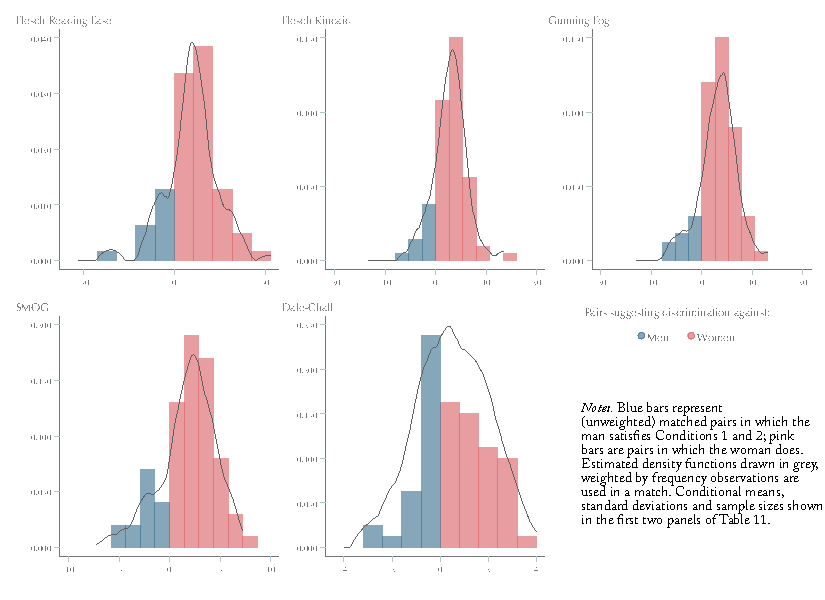
\includegraphics[width=12.3cm]{$HOME/Dropbox/Readability/draft/pdf/figure4.pdf}
	}
\end{figure}

\aref{appendixconservative} replicates \autoref{table10} using \autoref{equation12} to estimate $D_{ik}$. Results are very similar (and conclusions identical) to the analysis presented here.

\paragraph{Robustness}
\label{matchinglimitations}

Conclusions drawn from \autoref{table10} are principally predicated on two assumptions: (i) $i$ and $k$ are equivalent; (ii) $t$ is sufficiently large---\emph{i.e.}, $t>t'$ ($e_{nit}^s$ is on the convergence path to zero for $n=0,1$) and any errors in $i$'s beliefs about $\widetilde r_{0i}$ and $\widetilde R_i$ are sufficiently small.\footnote{\label{Footnote84}I use ``error'' and ``mistake'' to refer to anything that would cause authors to write more (or less) clearly than they would if $\widetilde r_{0i}^s$ and $\widetilde R_i^s$ were known. This includes actual mistakes in judgement as well as character components---\emph{e.g.}, conscientiousness or risk aversion---that impact beliefs and\slash or the optimal choice set under uncertainty.} If either is violated, discrimination against women cannot be inferred from an overrepresentation of matched pairs with $\underline D_{ik}>0$.

The first assumption depends on match accuracy. Post-match co-variates are well balanced (\aref{appendixmatchingbalance}). They remain well balanced---and similar to the matched population---when restricted to pairs satisfying $\underline D_{ik}>0$ and\slash or $\underline D_{ik}<0$ (\aref{appendixmatchingbalance}). To facilitate further scrutiny, \aref{appendixmatchingnames} lists the names of economists in each pair.

Matches are sensitive to the choice and construction of variables and the model and method used to estimate propensity scores. Outcomes, however, are not. After controlling for $T_i$, decade, journal and \emph{JEL} code, matches using alternative variables (\emph{e.g.}, minimum citation counts and mean institutional rank) and specifications (\emph{e.g.}, logit and no replacement) generate similar figures and conclusions. Results using a Mahalanobis matching procedure are shown in \aref{appendixmahalanobis}. Alternative specifications are available on request (\href{mailto:erin.hengel@gmail.com}{\texttt{erin.hengel@gmail.com}}).

The second assumption demands a ``sufficiently large'' $t$. For diagnosing discrimination, ``sufficiently large'' means $t'<3$ and the difference in $i$ and $k$'s error in beliefs at $t=3$ is smaller than $D_{ik}$. Forty-eight percent of all women with three or more top publications satisfy Conditions 1 and 2 when compared to equivalent men.\footnote{Women are the better writers in 73 percent of matched pairs. In 34 percent of those, however, the woman did not improve her writing between $t=1$ and $t=3$ (Condition 2), thus rendering \autoref{Theorem1}'s test for discrimination inconclusive.} Among them, $\underline D_{ik}$ is far from zero (\autoref{table10}, first column): these women write, on average, 29 percent more clearly than equivalent men with identical experience.\footnote{\autoref{table10}, first column divided by the mean male $\widehat R_{k3}$ (\aref{appendixconservative}).} It is unlikely that half of all female economists with three top publications---plus many more second-tier publications and substantial experience refereeing and editing themselves---make mistakes of this magnitude.

Interpreting $\underline D_{ik}$ as a causal, conservative estimate of discrimination's impact on readability requires the stronger assumption that $e_{ni3}^s=e_{nk3}^s$.\footnote{$\underline D_{ik}$ actually remains a causal, conservative estimate of the impact of discrimination against women under the weaker assumption $e_{ni3}^s\le e_{nk3}^s$, $n=0,1$ ($i$ female, $k$ male). See the proof of \autoref{Corollary1} in \aref{appendixproofs}.} When violated, I can no longer conclude that $\underline D_{it}$ conservatively estimates $D_{ik}$.\footnote{Specifically, this assumption is violated if at $t=3$ the women listed in \aref{appendixmatchingnames} make more (positive) mistakes about $\widetilde r_{0i}^s$ and\slash or $\widetilde R_i^s$ than the men they are matched to. For $\underline D_{ik}$ to remain a \emph{conservative} estimate of $D_{ik}$, women's mistakes must be no greater than men's mistakes at $t=3$.} Nevertheless, $e_{nit}^s-e_{nkt}^s$ is converging to zero and likely very small at $t=3$. Any upward bias from $e_{nkt}^s<e_{nit}^s$---\emph{i.e.}, from senior female economists \emph{still} making more mistakes about reviewers' thresholds than equivalent men even after previously publishing two top papers---is probably small and arguably offset by the downward bias already baked into $\underline D_{ik}$.\footnote{For a description of this downward bias, see the discussion on \autoref{Corollary1} in \autoref{seumodel} and the proof of \autoref{Corollary1} in \aref{appendixproofs}.}

Finally, causal interpretation technically requires that three additional criteria are also met. Assuming discrimination against $i$: (i) $i$'s acceptance rate is no more than $k$'s; (ii) $r_{0k3}\le r_{0i3}$---\emph{i.e.}, $i$'s draft readability is at least as high as $k$'s; and (iii) $r_{0i1}\le r_{0i3}$---\emph{i.e.}, $i$'s draft readability at $t=3$ is at least as high as his draft readability at $t=1$. As already discussed, (i) rules out the possibility that $i$ is appropriately rewarded (relative to $k$) for writing more clearly. (ii) and (iii) eliminate situations in which women write more clearly during peer review to compensate for poorer writing---and consequently higher desk rejection rates---before peer review.

Unfortunately, my data do not perfectly identify acceptance rates nor do I have $t=1$ and $t=3$ draft readability scores for every matched pair. Nevertheless, the data I do have and prior research strongly suggest (i)--(iii) not only hold on average, but do not exert upward bias on my estimate of $D_{ik}$, more generally. First, the previous section reviews the literature on gender neutrality in journals' acceptance rates. Women are not accepted more often than men. In \aref{appendixconservative}, I attempt to control for them explicitly by adding the requirement $T_i\le T_k$ or $T_k\le T_i$ to categorise matched pairs as discrimination against $i$ or $k$, respectively. Results are similar; conclusions unchanged. As shown in \autoref{nber}, women's draft papers are indeed more readable than men's. \autoref{indirecteffect} provides further confirmation. It plots the readability of women's and men's draft and published papers over increasing $t$. Women's drafts are more readable than men's drafts at $t=3$ \emph{and} more readable than their own earlier drafts at $t=1$.

\subsection{Indirect effect of higher standards}
\label{indirecteffect}

As a final exercise, I investigate how women react to higher standards as they update beliefs about referees' expectations. \autoref{figure6} compares papers pre- and post-review at increasing publication counts. Solid circles denote NBER draft readability; arrow tips reflect readability in the final, published versions of those same papers; dashed lines trace readability as papers undergo peer review. Figures are based on FGLS estimation of \autoref{equation14} (see \autoref{nber}):\begin{equation}\label{equation15}
	R_{itm} =	\beta_0 + \beta_1\,\text{female ratio}_{it} + \beta_2\,\text{female ratio}_{it}\times t_{it} + \beta_3\,t_{it} + \bm\uptheta\,\vect X_{it} + \varepsilon_{it},
\end{equation}where $m=W,P$ for working papers and published articles, respectively, and $\vect X_j$ is a vector of observable controls: editor, journal, year, journal and year interactions, English fluency dummies and quality controls---citation count and $\text{max. }T_j$. Since $t_i$ is author-specific, I disaggregate the data by duplicating each article $N_j$ times; to account for duplicate articles, regressions are weighted by $1/N_j$ (see \autoref{authorlevel}).\footnote{Results and conclusions based on unweighted regressions---or by replacing $t_i$ with $\text{max. }t_j$ and \emph{not} duplicating articles---are very similar or identical to those presented here. Regression output from alternative specifications available on request (\href{mailto:erin.hengel@gmail.com}{\texttt{erin.hengel@gmail.com}}).}

All things equal, economists who anticipate referees' demands are rejected less often; economists who don't enjoy more free time.\footnote{\label{Footnote132}Alternatively, if desk rejection rates are gender neutral, authors subjected to higher standards will undergo more arduous peer review. Greater scrutiny would therefore replace higher desk rejection rates when editors (or even referees) monitor and implement a policy of gender neutral acceptance rates.} \autoref{figure6} implies little---if any---gender difference in this tradeoff: senior economists of both sexes sacrifice time upfront to increase acceptance rates.

\begin{figure}
	
	\floatbox{figure}[\FBwidth]
	{
		\caption{Readability of authors' $t$th publication (draft and final versions)}\label{figure6}
	}
	{
		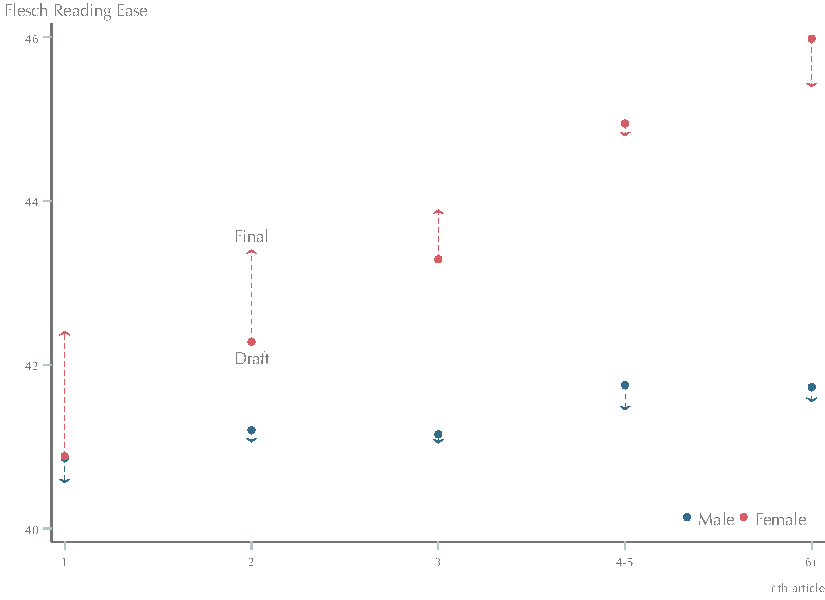
\includegraphics[width=12.3cm]{$HOME/Dropbox/Readability/draft/pdf/figure6.pdf}
		\floatfoot{\tiny \textit{Notes}. Sample 4,289 observations; 1,988 and 1,986 distinct NBER working papers and published articles, respectively; 1,840 distinct authors. Flesch Reading Ease marginal mean scores for authors' first, second, third, 4th--5th and sixth and up publications in the data. Solid circles denote estimated readability of NBER working papers from FGLS estimation of~\autoref{equation14}; arrow tips show the estimated readability in published versions of the same papers. Controls are: editor, year, journal, journal and year interactions, English fluency dummies and quality controls (citation count and $\text{max. }T_j$). Regression weighted by $1/N_j$. Pink represents women co-authoring only with other women; blue are men co-authoring only with other men.}
	}
\end{figure}

Moreover, \autoref{figure6} emphasises that only \emph{inexperienced women} improve readability during peer review.\footnote{Assuming no gender difference in acceptance rates at $t=3$ and given evidence that women are held to higher standards documented earlier, \autoref{figure6} suggests---but does not prove---that manuscripts by junior female economists are disproportionately rejected. See also \autoref{Footnote132} for an alternative interpretation in which acceptance rates are identical but scrutiny is not.} Assuming choices by senior economists express optimal tradeoffs with full information, this implies that women initially underestimate referees' expectations. Men, however, do not. Their draft and final readability choices remain relatively stable over increasing $t$.

Are men just better informed? Yes and no. Male and female draft readability scores for first-time publications are exactly the same, suggesting both start out with identical beliefs. Yet identical beliefs do not promise identical information. Men are indeed better informed because the standards they believe apply to them actually do. Female authors make the mistake in assuming those same standards apply to women, too.

The first panel of \autoref{table12} displays the magnitude and standard errors of the contemporaneous marginal effect of peer review ($R_{jP}-R_{jW}$) for men and women over increasing $t$. Estimates correspond to the lengths of the dotted lines in \autoref{figure6}. Gender differences are shown in the final row.

\begin{table}
    \footnotesize
    \centering
    \begin{threeparttable}
        \caption{Readability of authors' \(t\)th publication (draft and final versions)}
        \label{table12}
        \begin{tabular}{p{3cm}S@{}S@{}S@{}S@{}S@{}S@{}}
            \toprule
            &{\(t=1\)}&{\(t=2\)}&{\(t=3\)}&{\(t=4\text{--}5\)}&{\(t\ge6\)}\\
            \midrule
            \multicolumn{6}{l}{\textbf{Predicted \(R_{jP}-R_{jW}\)}}\\
            \quad Women                   &        1.51** &        1.12*  &        0.59   &       -0.15   &       -0.58   \\
                                          &      (0.64)   &      (0.60)   &      (0.70)   &      (0.89)   &      (1.16)   \\
            \quad Men                     &       -0.31*  &       -0.14   &       -0.11   &       -0.30** &       -0.18   \\
                                          &      (0.18)   &      (0.10)   &      (0.09)   &      (0.15)   &      (0.19)   \\
            \midrule\multicolumn{6}{l}{\textbf{Marginal effect of female ratio}}\\
            \quad Published article       &        1.82*  &        2.32***&        2.83***&        3.34***&        3.84***\\
                                          &      (1.03)   &      (0.74)   &      (0.74)   &      (1.05)   &      (1.48)   \\
            \quad Draft paper             &        0.00   &        1.06   &        2.13***&        3.19***&        4.25***\\
                                          &      (1.20)   &      (0.92)   &      (0.82)   &      (0.96)   &      (1.26)   \\
            \midrule
            \textbf{Difference}           &        1.82***&        1.26*  &        0.70   &        0.15   &       -0.41   \\
                                          &      (0.70)   &      (0.66)   &      (0.78)   &      (0.99)   &      (1.26)   \\
            \midrule
            Editor effects                &           {\ding{51}}   &           {\ding{51}}   &           {\ding{51}}   &           {\ding{51}}   &           {\ding{51}}   \\
            Journal effects               &           {\ding{51}}   &           {\ding{51}}   &           {\ding{51}}   &           {\ding{51}}   &           {\ding{51}}   \\
            Year effects                  &           {\ding{51}}   &           {\ding{51}}   &           {\ding{51}}   &           {\ding{51}}   &           {\ding{51}}   \\
            Journal\(\times\)Year effects          &           {\ding{51}}   &           {\ding{51}}   &           {\ding{51}}   &           {\ding{51}}   &           {\ding{51}}   \\
            Quality controls              &          {\(\text{\ding{51}}^5\)}   &          {\(\text{\ding{51}}^5\)}   &          {\(\text{\ding{51}}^5\)}   &          {\(\text{\ding{51}}^5\)}   &          {\(\text{\ding{51}}^5\)}   \\
            Native speaker                &           {\ding{51}}   &           {\ding{51}}   &           {\ding{51}}   &           {\ding{51}}   &           {\ding{51}}   \\
            \bottomrule
        \end{tabular}
        \begin{tablenotes}
            \tiny
            \item \textit{Notes}. Sample 4,289 observations; 1,988 and 1,986 distinct NBER working papers and published articles, respectively; 1,840 distinct authors. Panel one displays magnitude of predicted \(R_{jP}-R_{jW}\) (the contemporaneous effect of peer review) for women and men over increasing publication count (\(t\)). Panel two estimates the marginal effect of an article's female ratio (\(\beta_1+\beta_2\)), separately for draft papers and published articles. Figures from FGLS estimate of~\autoref{equation14}. Quality controls denoted by \(\text{\ding{51}}^5\) include citation count and \(\text{max. }T_j\). Standard errors clustered by editor and robust to cross-model correlation in parentheses. ***, ** and * statistically significant at 1\%, 5\% and 10\%, respectively.
        \end{tablenotes}
    \end{threeparttable}
\end{table}

For publications $t=1$ and $t=2$, differences are large, positive and significant; for publications three and up, they're fairly small. Nevertheless, the readability gap in the published article remains large, statistically significant and relatively stable at every $t$ (\autoref{table12}, second panel). Increasingly, however, it forms before submission. Draft readability contributes nothing to the gap at $t=1$. That rises to 43 percent at $t=2$ and 73 percent at $t=3$. By $t=4\text{--}5$ and $t=6+$, men and women mostly choose to address referee concerns prior to peer review, corroborating analysis based on \autoref{figure6}. 

\autoref{figure6} and \autoref{table12} document evidence that female economists are held to relatively constant---albeit higher---standards throughout their careers. Over time, women adjust to those standards by writing more clearly before peer review. Assuming---as other evidence suggests---that women's papers are accepted no more often than men's papers, this implies that female economists at every level of seniority must work harder than their male peers to achieve a similar outcome.

\paragraph{Impact on identifing discrimination}
\label{identificationimpact}

\autoref{figure6} supports \autoref{Theorem1}`s implicit assumption that female authors learn about referees' thresholds over time. If the payoff from lucid exposition is high, people will catch on---either by internalising explicit comments on text readability in referee reports from earlier papers or making the (un)conscious connection that acceptance rates are higher---or review times are faster---when text is clearer. Applying that payoff only to women yields a succinct explanation for the gap's observed growth.

Although \autoref{table12} concurs, viewing certain estimates in isolation give different, more orthodox impressions. First, panel one suggests that the readability gap declines over increasing $t$. This narrow view favours alternative explanations---\emph{e.g.}, sensitivity, poor information and\slash or justified statistical discrimination---over bias by referees and\slash or editors. Only when complemented by \autoref{figure6} do we fully appreciate that the smaller gap \emph{in} peer review is completely offset by a wider gap \emph{before} peer review. Unfortunately, this reaction poses another identification problem: senior female economists adjust to biased treatment in ways that confuse underlying discrimination with voluntary choice. Both observations suggest that studies must account for all relevant decisions at a single point in time \emph{and} the evolution of those decisions over time. Otherwise, they may underestimate discrimination and misallocate responsibility.\footnote{This study suffers from the same criticism. For example, it does not take into account the impact higher standards have on (potential) female economists' choice of field, specific topic or even their decisions to remain in the workforce.} 

\subsection{Duration of peer review}
\label{duration}

``Writing simply and directly only looks easy''~\citep[][p. 53]{Kimble1994}. An essay's rhetorical competency is highly correlated with the length of time one is given to compose it~\citep{Hartvigsen1981,Kroll1990}. Skilled writers spend more time contemplating a writing assignment, brainstorming and editing. They also write fewer words per minute and produce more drafts~\citep{Faigley1981,Stallard1974}.

Since writing simply and directly takes time, one observable repercussion will be prolonged peer review for female authors. To investigate, I turn to \emph{Econometrica}, the only journal to make disaggregated data on the revision process publicly available.

\autoref{figure5} is a histogram of time (in months) between dates papers are first submitted to and their final revisions received by \emph{Econometrica}'s editorial office. Blue bars represent articles written only by men, pink bars are those just by women. The 180 papers co-authored by men and women are not included.

\begin{figure}
	
	\floatbox{figure}[\FBwidth]
	{
		\caption{Distribution of review times at \textit{Econometrica}}\label{figure5}
	}
	{
		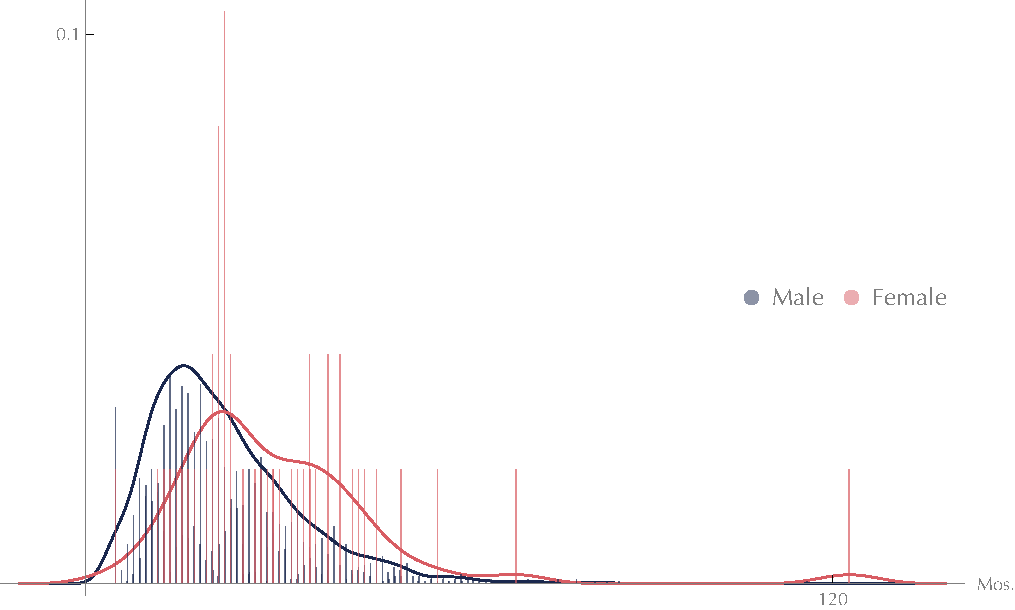
\includegraphics[width=12.3cm]{$HOME/Dropbox/Readability/draft/pdf/figure5.pdf}
		\floatfoot{\tiny \textit{Notes}. Sample 2,446 articles. Bars are proportional to the number of papers published in \textit{Econometrica} with a given review time (months between first submission and final acceptance). Blue bars represent papers written only by men (2,397); pink bars are papers written only by women (49). Source: \textit{Econometrica}.}
	}
\end{figure}

Since 1950, \emph{Econometrica} published 53 papers authored entirely by women.\footnote{Submit-accept times were not available for four of these articles (see \autoref{data}).} As \autoref{figure5} illustrates, their review times disproportionately cluster in the distribution's right tail: articles by women are six times more likely to experience delays above the 75th percentile than they are to enjoy speedy revisions below the 25th.\footnote{Three out of four of the papers with the longest peer review are authored by at least one woman. Almost a quarter of the papers that took longest in peer review post 2000 had at least one female author.}

For a more precise appraisal, I build on a model by  \citet[][Table 6, p. 963]{Ellison2002a} and estimate \autoref{equation13}:\begin{equation}\label{equation14}
	\widehat R_{it} = \alpha_{tg_i} + \beta_{tg_i}\,\text{female ratio}_{it} + \varepsilon_{it},
\end{equation}where $\text{mother}_j$ and $\text{birth}_j$ are binary variables equal to 1 if article $j$'s authors were all mothers to children younger than five and gave birth, respectively, at some point during peer review,\footnote{If one co-author goes on maternity leave or has young children, I assume another co-author manages the revision process unless she, too, faces similar family commitments.} $\max t_j$ is the number of prior papers published in any of the top four economics journals by article $j$'s most prolific co-author, $\text{no. pages}_j$ refers to the page length of the published article, $\text{order}_j$ is the order in which article $j$ appeared in an issue and $\text{no. citations}_j$ are the number of subsequent papers citing $j$.\footnote{I control for all significant factors identified by  \citet{Ellison2002a}. His work evaluates whether author compositional effects contributed to higher mean-accept times at \emph{AER}, \emph{Econometrica}, \emph{JPE}, \emph{QJE} and the \emph{Review of Economic Studies}.}

\begin{table}
    \begin{adjustwidth}{-0.085cm}{}
    \footnotesize
    \centering
    \begin{threeparttable}
        \caption{Revision duration at \textit{Econometrica}}
        \label{table11}
        \sisetup{round-precision=3,table-format=3.4}
        \begin{tabular}{p{2.64cm}SSSSSSS}
            \toprule
            &{(1)}&{(2)}&{(3)}&{(4)}&{(5)}&{(6)}&{(7)}\\
            \midrule
            Female ratio                  &       5.436** &       6.635***&       6.641***&       5.708***&       6.657***&       8.766***&       8.800***\\
                                          &     (2.065)   &     (2.165)   &     (2.146)   &     (2.114)   &     (2.150)   &     (2.678)   &     (2.714)   \\
            Max. \(t_j\)                  &      -0.163** &      -0.169** &      -0.164** &      -0.163** &      -0.163** &      -0.163*  &      -0.169*  \\
                                          &     (0.070)   &     (0.071)   &     (0.070)   &     (0.070)   &     (0.070)   &     (0.087)   &     (0.087)   \\
            No. pages                     &       0.180***&       0.179***&       0.178***&       0.180***&       0.178***&       0.219***&       0.207***\\
                                          &     (0.026)   &     (0.026)   &     (0.026)   &     (0.026)   &     (0.026)   &     (0.040)   &     (0.042)   \\
            \(N\)                         &       1.016** &       0.977** &       0.966** &       1.002** &       0.974** &       1.220*  &       1.158   \\
                                          &     (0.444)   &     (0.441)   &     (0.442)   &     (0.444)   &     (0.442)   &     (0.687)   &     (0.696)   \\
            Order                         &       0.223** &       0.221** &       0.218** &       0.222** &       0.219** &       0.516** &       0.493** \\
                                          &     (0.089)   &     (0.090)   &     (0.089)   &     (0.089)   &     (0.089)   &     (0.215)   &     (0.218)   \\
            No. citations                 &       0.000   &       0.000   &       0.000   &       0.000   &       0.000   &      -0.003** &      -0.004***\\
                                          &     (0.000)   &     (0.000)   &     (0.000)   &     (0.000)   &     (0.000)   &     (0.001)   &     (0.001)   \\
            Mother                        &               &               &      -6.280** &               &     -10.677***&     -18.451***&     -18.338***\\
                                          &               &               &     (2.698)   &               &     (3.381)   &     (3.527)   &     (3.673)   \\
            Birth                         &               &               &               &      -2.409   &       7.321*  &      13.525** &      12.982** \\
                                          &               &               &               &     (3.380)   &     (4.268)   &     (5.277)   &     (5.593)   \\
            Constant                      &      37.727***&      37.584***&      37.787***&      37.710***&      37.880***&      14.223***&      14.884***\\
                                          &     (2.040)   &     (2.078)   &     (2.044)   &     (2.050)   &     (2.055)   &     (2.888)   &     (2.793)   \\
            \midrule
            Editor effects                &           {\ding{51}}   &           {\ding{51}}   &           {\ding{51}}   &           {\ding{51}}   &           {\ding{51}}   &           {\ding{51}}   &           {\ding{51}}   \\
            Year effects                  &           {\ding{51}}   &           {\ding{51}}   &           {\ding{51}}   &           {\ding{51}}   &           {\ding{51}}   &           {\ding{51}}   &           {\ding{51}}   \\
            Institution effects           &           {\ding{51}}   &           {\ding{51}}   &           {\ding{51}}   &           {\ding{51}}   &           {\ding{51}}   &           {\ding{51}}   &           {\ding{51}}   \\
            \textit{JEL} (primary) effects&               &               &               &               &               &               &           {\ding{51}}   \\
            No. observations              &       2,626   &       2,611   &       2,626   &       2,626   &       2,626   &       1,281   &       1,281   \\
            \bottomrule
        \end{tabular}
        \begin{tablenotes}
            \tiny
            \item \textit{Notes}. Sample 2,626 articles. Coefficients from OLS estimation of~\autoref{equation13}; (2) excludes papers authored only by women who gave birth (7 articles) and/or had a child younger than five (9 articles) at some point during peer review. Standard errors clustered by year in parentheses. ***, ** and * statistically significant at 1\%, 5\% and 10\%, respectively.
        \end{tablenotes}
    \end{threeparttable}
    \end{adjustwidth}
\end{table}

\autoref{table11} displays results across a range of specifications. Column (1) does not control for motherhood or childbirth; (2) drops papers authored by women who had children younger than five and\slash or gave birth during peer review; (3) controls for motherhood but not childbirth; (4) controls for childbirth but not motherhood; (5) controls for both childbirth and motherhood; (6) includes fixed effects for primary \emph{JEL} categories.\footnote{\emph{JEL} classifications are only available for papers published after 1990 (see \autoref{data}); \autoref{table11}'s column (6) estimates \autoref{equation13} on only half of the data.}

Every paper published in \emph{Econometrica} undergoes extensive review, but the consistently large and highly significant coefficient on female ratio suggests women bear the worst of it.\footnote{This conclusion is robust to altering the age-threshold on $\text{mother}_j$ (see \aref{appendixmotherhood}).} The average male-authored paper takes 18.5 months to complete all revisions; papers by women need more than half a year longer.\footnote{\label{Footnote88}Based on results in (5). Male effect estimated with zero female co-authors (standard error 0.102). When publication year fixed effects are replaced with submission year fixed effects, female-authored papers spend about four months longer in peer review (see \aref{appendixsubmissionyear}).}

Why? Well, it's not motherhood. Yes, giving birth slows down review---responding to referees is apparently put on hold for the first year of a newborn's life---but having a young child has the opposite effect. A pause for childbirth is expected; a productivity boost from pre-schoolers is not. Perhaps wanting to spend time with the kids motivates women to get organised? Or, maybe the most organised women are the only ones having children? The former suggests motherhood is not the productivity killer it's rumoured to be---at least among highly educated women. The latter implies only superstar women feel academic careers and motherhood are simultaneously manageable.\footnote{A third hypothesis is that referees (possibly responding to editors) demand fewer revisions when women have young children. Because reviewers are unlikely to have this information---based on my own experience, it is remarkably difficult to find out---I (perhaps unfairly) give this interpretation less weight.} Both interpretations are provocative, but should be made with caution given (i) counter-intuitive results, (ii) obtaining an unbiased estimate of $\beta_2$ was \emph{not} this study's objective and (iii) $\text{mother}_j$ equals one for only 16 articles in the sample.\footnote{The count increases to 17 and 19 articles when $\text{mother}_j$'s threshold is defined as children younger than ten and 18, respectively (see \aref{appendixmotherhood}).}

As for \autoref{table11}'s remaining coefficients, all are significant or highly significant and correspond to earlier estimates by  \citet{Ellison2002a}. Longer papers take more time to review, as do papers with more co-authors and those that appear earlier in an issue. Authors with an established publication history and highly cited papers (possibly) enjoy marginally faster reviews.\footnote{\citet{Ellison2002a}'s analysis includes a dummy variable for female authorship; it is positive post--1990 but not significant (it is negative and insignificant before that). His paper does not discuss the finding.} 

\section{Discussion}
\label{discussion}

A gender readability gap exists. It's still there after including editor, journal and year effects---meaning we cannot blame specific policies or attitudes in the 50s, long since overcome. The gap is unaffected by field controls, so it's not that women research topics that are easier to explain. Perhaps it's caused by factors correlated with gender but actually linked to authors' (or co-authors') competence as economists or fluency in English? If so, institution and native speaker dummies would reduce it. They do not.\footnote{I also conducted a primitive surname analysis ~\citep[see][pp. 35--36]{Hengel2016}. It suggests that the female authors in my data are no more or less likely to be native English speakers.}

The gap grows between first draft and final publication and over the course of women's careers. This precludes systemic bias by article- or author-specific fixed effects---\emph{e.g.}, inborn advantages and one-off improvements in response to external circumstances unrelated to peer review.

It likewise rules out gender differences in (i) biology\slash behaviour---\emph{e.g.}, sensitivity to referee criticism\footnote{While women do appear more \emph{internally} responsive to feedback---criticism has a bigger impact on their self-esteem---available evidence suggests they aren't any more \emph{externally} responsive to it, \emph{i.e.}, women and men are equally likely to change behaviour and alter performance after receiving feedback~\citep{Johnson2002,Roberts1989}.}---or (ii) knowledge about referee expectations. If diligently addressing every referee concern has no apparent upside---acceptance rates are unaffected---and a very clear downside---constant redrafting takes time---shouldn't even oversensitive, ill-informed women \emph{eventually} re-examine beliefs{\ldots} and start acting more like men (\autoref{Theorem1})? Yet this is not what we observe. The largest investments in writing well are made by female economists with greatest exposure to peer review---\emph{i.e.}, those with the best opportunity to update their priors.

Women's papers are more likely assigned female referees~\citep{Abrevaya2012,Gilbert1994}.\footnote{Note that women are only a fraction of all referees---8 percent in 1986~\citep{Blank1991}, 10 percent in 1994~\citep{Hamermesh1994} and 14 percent in 2013~\citep{Torgler2013}.  \citet{Abrevaya2012} report female-authored papers were only slightly more likely to be assigned a female referee between 1986--1994, although matching does increase in 2000--2008.} If female referees are more demanding critics, clearer writing could reflect their tougher reviews.\footnote{It's not so clear whether their reports are any more critical. A study specific to post-graduate biologists suggests yes~\citep{Borsuk2009}; another analysing past reviews in an economics field journal does not~\citep{Abrevaya2012}.} Women concentrate in particular fields, so it's natural their papers are more often assigned female referees. However, for the readability gap to exist only because of specialisation, controlling for \emph{JEL} classification should explain it.\footnote{Specifically, men and women publishing in the same field face the same pool of referees. Controlling for that pool would account for gender differences in readability.} It does not. In fact, even including 718 tertiary \emph{JEL} category dummies has virtually no effect. So if referee assignment is causing the gap, it's only because journals disproportionately refer female-authored papers to the toughest critics. Meaning it isn't referees who are biased---it's editors.\footnote{This is a form of biased referee assignment (\autoref{Theorem1}). A similar argument contends that female research is more provocative, and more provocative work warrants more scrutiny. If this were true, controlling for \emph{JEL} classification would also reduce (or eliminate) the gap---unless women's work is systematically more provocative even among researchers in very narrow fields. Yet provocative work is (presumably) highly cited work, and there is no discernible gender difference in citation counts~\citep{Ceci2014}. Alternatively, perhaps the wider public excessively scrutinises female work, and referees respond similarly to minimise blowback. This explanation assumes a wider public capable of discrediting our work---a view many economists would (privately) disagree with. In any case, economics employs advanced mathematics and technical language, making it especially inaccessible to a layperson.}

A final alternative is rather uncomfortable. Perhaps female-authored manuscripts deserve more criticism because they aren't as good? As mentioned earlier, factors correlated with gender but actually related to competency should decline when appropriate proxies are included. The sample itself is one such proxy---these are, after all, only articles published in the top four economics journals. Adding other controls---author institution, total article count, citation counts and published order in an issue---has no effect.\footnote{Published order in an issue refers to the order an article appears in a particular issue (\emph{i.e.}, one for the lead article, two for the second article, \emph{etc.}). This control was introduced as a a set of indicator variables. See  \citet[][p. 42 and p. 44]{Hengel2016} for regression output.} The gap is widest for the most productive economists and even exists among articles originally released as NBER working papers---both presumably very clear signals of merit.

Yet I cannot rule out the possibility that women's work is systematically worse than men's---or that the female and male authors in \autoref{seumatching} are not really equivalent. (To decide for yourself, see \aref{appendixmatchingnames}.) And if this is true, referees \emph{should} peruse our papers more carefully---a byproduct of which could be better written papers after-the-fact or more attractive prose compensating for structural weaknesses before it.\footnote{It does seem contradictory, however, that women would be capable of writing better than men---even before referee input (\autoref{table7})---but incapable of producing similar quality research. One is inclined to believe clarity of thought and quality of research to go hand-in-hand, although I am not aware of any study on the topic.}

``Quality'' is subjective; measurement, not easy. Nevertheless, attempts using citation counts and journal acceptance rates do not indicate that men's research is any better: as discussed in \autoref{seumodel}, gender has virtually zero impact on the latter;\footnote{Journals may have a policy of publishing female-authored research over equal (or even better) male work. If so, acceptance rates are not an unbiased indicator of quality.} a review of past studies on male vs. female citations find four in which women's papers received fewer, six where they were cited more and eight with no significant difference~\citep{Ceci2014}.

More complicated, multi-factor explanations could resolve inconsistencies present when each is analysed in isolation. Perhaps female economists are perfectionists, and it gets stronger with age?\footnote{While women score higher on maintaining order~\citep{Feingold1994}---a trait including organisation and perfectionism---significant differences are not universally present in all cultures~\citep{Costa2001}. Moreover, differences that are present decline---or even reverse---as people age~\citep{Weisberg2011}.} Maybe women actually enjoy being poorly informed, overconfident and sensitive to criticism---or (more likely) I may have otherwise misspecified the author's objective function in \autoref{seumodel}. It is also possible that the statistically significant relationships this paper documents are unfortunate (particularly for me!) flukes.

Still, no explanation matches the simplicity and believability of biased referees and\slash or editors. Coherence and economy do not establish fact, but they are useful guides. This single explanation neatly accounts for all observed patterns. If reviewers apply higher standards to female-authored papers, those papers undergo more thorough review. Added scrutiny should improve women's exposition but lengthen review times---as seen in \autoref{duration}. The rewards from clearer writing are presumably internalised, meaning women gradually improve---which they do, as illustrated in \autoref{experience}.

Moreover, several studies document a gender difference in critical feedback of similar form---employee performance reviews and student evaluations.\footnote{No one (to my knowledge) has tested whether men and women receive different critical feedback in peer review reports,} Ongoing research suggests female workers are held to higher standards in job assessments. They are acknowledged less for creativity and technical expertise, their contributions are infrequently connected to business outcomes; guidance or praise supervisors do offer is vague~\citep{Correll2016}.\footnote{A similar phenomenon exists in online fora. The \emph{Guardian} commissioned researchers to study 70 million comments on its website. It found female and black writers attract disproportionately abusive threads~\citep{Gardiner2016}.}

Students display a similar bias. \href{http://benschmidt.org/profGender/}{Data} from \href{http://www.ratemyprofessors.com/}{Rate My Professors} suggest female lecturers should be ``helpful'', ``clear'', ``organised'' and ``friendly''. Men, instead, are praised (and criticised) for being ``smart'', ``humble'' or ``cool''~\citep{Schmidt2015}.\footnote{These conclusions are based on an observational account of the data.} A study of teaching evaluations similarly finds students value preparation, organisation and clarity in female instructors; their male counterparts are considered more knowledgable, praised for their ``animation'' and ``leadership'' and given more credit for contributing to students' intellectual development~\citep{Boring2017}.

TO ADD:

Readability scores may be capturing something not related to readability.

Readability scores may be capturing the fact that referees are less interested in female work. This suggests a systematic bias against women in peer review, but is not necessarily the \emph{fault} of individual referees. Instead, it just reflects another---albeit no less insiduous---bias taht results from systematic underrepresentation of women. However, the readability gap remains after controlling for detailed \emph{JEL} codes. Thus, this must mean that referees are systematically less interested in women's work even after controlling for highly specific sub-fields. That is, male-authored papers are more appealing to editors and referees even compared to female-authored papers in the exact same field.

The readability of text may be more important when interest is low than when it is high~\citep{Klare1976,Fass1978}. It has also been shown that prior knowledge and beliefs about a topic improved reading comprehension for a particular text~\citep{Woern1977,Spilich1979,Chiesi1979}. Easier readability of a text has more benefits for those of less knowledge and interest than those of more. Advanced knowledge of a subject can ``drown out'' the effects of an otherwise difficult text. This study also suggested that when reader interest is high, comprehension is not improved by writing the material below, rather than at, the grade level of the readers. When interest is low, however, comprehension is improved by writing the materials below, rather than at, the reading level of the readers.

A remaining concern is whether peer review actually affects manuscript readability. In a review of prestigious biomedical journals,  \citet{Boutron2016} find that 47 percent of editors clearly request that referees evaluate the language of a manuscript they are reviewing. Additionally, a review of the comments posted on ShitMyReviewer.com, quarter deal with writing quality, document structure or word choice\slash tone (FIGURE XXXXX).

Thus underlying all of the conclusions presented in this paper is the implicit assumption that if some perfect measure of readability existed that incorporated these factors, it would conclude the same thing. Thus assumption implies that the effects presented in this paper suffer from attenuation bias.\footnote{An alternative bias is instead the ``file drawer bias''---\emph{i.e.}, all the other studies showing no effect just don't get published. I try to counteract this effect by collecting a relatively large sample. Nevertheless, the required sample size necessarily depends on the number of female authors, of which there are not very many. Thus, the possibility that the effects I observe in \emph{three separate samples} are just statistical flukes can not be ruled out.} given the relatively large textual samples used in the paper, the effects presented in fact suffer from attenuation bias.

Because readability scores omit these factors using them to infer causality between gender and any outcome they attempt to proxy for implicitly assumes that gender impacts these other facets in the same way that gender impacts readability. Or, in other words, if we \emph{did} have a more comprehensive measure of readability, it would show the same thing.

And in any case, readability scores are perfect (or almost perfect) predictors of sentence and word length. Thus, the figures presented in this paper will always capture differences in the weighted averages of these two measures.

I do not measure ``quality'' with readability. Quality is multidimensional and in any way highly subjective---I challenge anyone to find more than two people to agree on the components most important to quality. Nevertheless, if readability is an unbiased proxy for it, then these results suggest women's papers are in fact higher quality.

\emph{Discuss classicial measurement error vs. non-classical measurement error}.

Classical measurement error is of most concern in small sample sizes with a high degree of variability between individuals because higher weights are placed on individual results. While I cannot rule out classical measurement error entirely as a factor driving my results, the fact that sample sizes are both relatively large and results do not appear to be driven by any individual results, suggests it is probably not, on its own, a particularly important factor.

Thus, if non-classical measurement error prevents inferring gender differences in \emph{readability} it is still the case that sentence-length and vocabulary complexity in female-authored papers is negatively affected by peer review. 

Thus, should non-classical measurement error prevent inferring readability between genders, one must nevertheless confront the observation that sentence-length and vocabulary complexity in female-authored papers is negatively affected by peer review. 

The weighted average of these two variables is informative in much the same way that the general ``readability'' inference may be.

\subsection{Open review}
\label{openreview}

Academia's female productivity gap is as stubborn as the business world's pay gap; yet, if every paper a woman writes needs \textbf{\emph{six more months}} to finish review, our ``Publishing Paradox'' seems much less paradoxical.\footnote{\label{footnote77}Virtually every study on gender differences in scientific publishing rates find men more productive than women~\citep[for a list, see][]{Ceci2014}. It's no different in my data: women published on average 1.7 articles; men managed 2.4---and with far more concentration in the distribution's right tail (for example, 56 men have published 16 or more times in the data, but no woman). Women produce fewer papers even when they don't have any children~\citep{Ceci2014}. Appropriate controls for teaching and service do not account for it~\citep{Xie2005}, and it isn't a question of time, since female academics work just as many hours as men~\citep{Ceci2014,Ecklund2011}.}

Is the answer double-blind review? Probably not. Double-blind review cannot stop referees from guessing authors' identities---which they did with surprising accuracy before the internet~\citep{Blank1991}, and presumably perfect accuracy after it.

Instead, eliminate single-blind review, too. A randomised controlled trial at the \emph{British Journal of Psychiatry} suggests referee reports are better quality and less abusive when identities are known~\citep{Walsh2000}. Posting them online---as the \emph{British Medical Journal} does---virtually guarantees continuous, independent audits by outside researchers.\footnote{The \emph{BMJ} posts reviewers' signed reports, authors' responses and the original manuscript on its website. No documentation is posted for rejected papers, but doing so may be beneficial: (i) A very public review implies a very public rejection; concern for one's reputation could reduce the number of low quality submissions. (ii) The onus of discovering mistakes would be shared with the wider economics community. (iii) Other journals can make publication decisions based on posted reviews---possibly reducing time spent refereeing for the discipline, as a whole. Women may receive greater scrutiny online---as they do at the \emph{Guardian}~\citep{Gardiner2016}---but the difference can be mitigated if comments are non-anonymous, made only by verified members of an appropriate professional society and continuously (and publicly) audited for bias in quantity and quality of feedback.} Worries that reviews are less critical and\slash or relationships are strained are either unfounded or alleviated by the deep pool of referees common to general interest journals~\citep{vanRooyen1999,vanRooyen2010}. Open review does incur costs---some people refuse to participate and those that don't spend marginally more time drafting reports~\citep{vanRooyen1999,Walsh2000}\footnote{Each study employed a different research design; nevertheless, both estimate roughly 12 percent of reviewers decline to participate because they oppose open peer review while signing reports increases time spent on the review by 25 minutes. When referees were told their signed reviews might be posted online, time rose by an additional half hour and refusal rates were much higher (55 percent)~\citep{vanRooyen2010}.}---but if more accountability promotes fairer outcomes, ethical arguments in its favour should outweigh minor practical concerns.

\section{Conclusion}
\label{conclusion}

This paper makes a curious discovery: female-authored articles in top economics journals are better written. After examining the difference, I conclude that higher standards applied by editors and\slash or referees are primarily to blame.

No prior study has uncovered convincing evidence of gender bias in journal acceptance rates. It's encouraging that sex is irrelevant to publication outcomes, but that does not mean it has no effect on the process---or on the productivity of female academics. When female authors endure unfair criticism in referee reports, clearer writing and longer review times follow. With less time to spend on new projects, research output slows down.

Higher standards impose a quantity vs. quality tradeoff that not only reconciles academia's ``Publishing Paradox'', but also rationalises many instances of female output. Work that is evaluated more critically at any point in the production process will be systematically better (holding prices fixed) or systematically cheaper (holding quality fixed). This reduces women's wages---for example, if judges require better writing in female-authored briefs, female attorneys must charge lower fees and\slash or under-report hours to compete with men---and distorts measurements of female productivity---billable hours and client revenue decline; female lawyers appear less productive than they truly are.

Finally, the topic of my study is narrow, but its methodology has wider applications. To the best of my knowledge, this paper is the first (in economics) to identify discrimination using the choices and behaviours of those discriminated against. Although applied to a specific context---peer review---the identifying logic equally suits any situation where people repeatedly receive and act on biased feedback. Moreover, this study is also the first to uncover subtle group differences with readability scores.\footnote{\label{footnote81} \citet{Ali2010} identified readability scores as useful tools for social scientists. In a large scale analysis of news content, they found stories on sports (male dominated) and entertainment (female dominated) most readable.  \citet{Stempel1981} reports similar findings in popular U.S. newspapers.} These scores are not new---all are extensively tested with well-documented properties---but their use is mostly confined to determining whether text is appropriate for intended audiences.\footnote{\label{footnote82} \citet{Long2011},  \citet{Lehavy2011} and  \citet{Thörnqvist2015} use readability scores in interesting, non-conventional ways. The former investigates whether a legal brief's Flesch Reading Ease score is correlated with its success on appeal (it is not); the latter two use readability measures to proxy for complex information in financial reports, finding less readable material is less informative~\citep{Lehavy2011}, especially for non-sophisticated investors~\citep{Thörnqvist2015}. Since releasing the first version of this working paper (September, 2015) research using readability scores has ballooned. See \citet{Benoit2017} for a review of more recent research.} As this paper demonstrates, however, readability scores are also effective tools to evaluate asymmetry anywhere ideas are communicated orally or in writing and large amounts of source material are easily obtainable: journalism, speeches, student essays, business plans, Kickstarter campaigns, \emph{etc.} Research potential is substantial.


% Affiliation at end.
\ifaffiliationend
    \vspace*{0.5cm}
    \indent\textit{\department, \affiliation, \address.}
\fi

% Bibliography before appendix
\ifappendixlast
    \begin{SingleSpace}
        \printbibliography[heading=subbibliography]
    \end{SingleSpace}
\fi

% Tables/figures at end.
\iftableslast
    \makeatletter
    \efloat@restorefloats
    \makeatother
\fi
\clearpage
\begin{appendices}



\section{Proofs}
\label{appendixproofs}

The proof of \autoref{Theorem1} follows directly from \autoref{Lemma5}, at the end of this section. The proof of \autoref{Lemma5} relies on a series of additional lemmas stated and proved below. Throughout, $\{(r_{0it},R_{it})\}$ represents the sequence of readability choices made by author $i$ for all $t$. $R_i^\star$ is defined as the $R$ that solves $\phi_i'(R)=c_i'(R)$. Review group $s$ is referred to as ``state $s$''.

% Lemma 1.
\begin{lemma}\label{Lemma1}
	$\{(r_{0it}, R_{it})\}$ is bounded.
\end{lemma}
\begin{proof}
Consider the sequence of initial readability choices, $\{r_{0it}\}$. I first show that $R_i^\star\le r_{0it}$ for all $t$. Recall $r_{0it}$ is chosen to maximise the author's subjective expected utility in~\autoref{equation9}. It satisfies the following first order condition
\begin{equation}\label{equationA1}
	\int_\Sigma\!\left(\pi_{0it}^s(r_{0it})v_{1it}^s+\Pi_{0it}^s(r_{0it})\frac{\pd v_{1it}^s}{\pd{r_{0it}}}\right)\dd\mu_i+\phi_i'(r_{0it})-c_i'(r_{0it})=0,
\end{equation}
where $v_{1it}^s$ represents \autoref{equation9} evaluated at the optimal $r_{1it}$. $\phi_{i|r_{0it}}(r_{1it})=\phi_i(R_{it})-\phi_i(r_{1it})$ and $c_{i|r_{0it}}(r_{1it})=c_i(R_{it})-c_i(r_{0it})$. Thus,
\begin{align}\label{equationA2}
	\frac{\pd v_{1it}^s}{\pd r_{0it}}&=\pi_{1it}^s(R_{it})u_i+\phi_i'(R_{it})-c_i'(R_{it})-\phi_i'(r_{0it})+c_i'(r_{0it})\nonumber\\
	&=\frac{\pd v_{1it}^s}{\pd r_{1it}}+c_i'(r_{0it})-\phi_i'(r_{0it}).
\end{align}

Since $\phi_i'(R_i^\star)=c_i'(R_i^\star)$, $\pd v_{1it}^s/\pd r_{0it}=\pd v_{1it}^s/\pd r_{1it}$ when evaluated at $r_{0it}=R_i^\star$. The left hand side of~\autoref{equationA1} evaluated at $r_{0it}=R_i^\star$ is correspondingly equivalent to
\begin{equation}\label{equationA3}
	\int_\Sigma\!\left(\pi_{0it}^s(r_{0it})v_{1it}^s+\Pi_{0it}^s(r_{0it})\frac{\pd v_{1it}^s}{\pd r_{1it}}\right)\dd\mu_i.
\end{equation}
$v_{1it}^s$ is non-negative;\footnote{\autoref{equation8} evaluated at $r_{1it}=0$ is non-negative. Since $r_{1it}$ maximises~\autoref{equation8}, $v_{1it}^s$ is likewise non-negative.} optimising behaviour at stage 1 implies $\pd v_{1it}^s/\pd r_{1it}\ge0$: either an $r_{1it}$ exists that satisfies $\pd v_{1it}^s/\pd r_{1it}=0$, or the author chooses $r_{1it}=0$ and $\pd v_{1it}^s/\pd r_{1it}=\pi_{1it}^s(R_{it})u_i$ is non-negative. Thus,~\autoref{equationA3} is non-negative. Since $c_i'(r)<\phi_i'(r)$ for all $r<R_i^\star$, the left-hand side of~\autoref{equationA1} is strictly positive for all $r<R_i^\star$, so $r_{0it}$ must be at least as large as $R_i^\star$.

I now show that $\{r_{0it}\}$ is bounded from above. As $r_{0}$ tends to infinity, authors choose not to make any changes at stage 1. Thus,
\begin{equation}\label{equationA4}
	\lim_{r_0\rightarrow\infty}\,\Pi_{0it}^s(r_0)v_{1it}^s=\overline\Pi_{0it}^s\overline\Pi_{1it}^s u_i,
\end{equation}
where $\overline\Pi_{0it}^s$ and $\overline\Pi_{1it}^s$ are some upper bounds on the author's subjective probability of receiving an R\&R and then being accepted in state $s$ at time $t$. Since both are no more than 1, $u_i$ is finite and $\phi_i(r)-c_i(r)$ is strictly decreasing for all $r>R_i^\star$,
\begin{equation}\label{equationA5}
	\lim_{r_0\rightarrow\infty}\left\{\int_\Sigma\!\Pi_{0it}^s(r_0)v_{1it}^s\,\dd\mu_i+\phi_i(r_0)-c_i(r_0)\right\}=-\infty.
\end{equation}

Similarly, because $\Pi_{0it}^s(r_{0it})\Pi_{1it}^s(R_{it})\le1$ for all $s$ and $\phi_i(r)$ and $c_i(r)$ are finite at all $r<\infty$,~\autoref{equation9} is likewise finite for all $r<\infty$. Thus,
\begin{equation*}
	\sup\left\{\argmax_{r_{0it}}\,\int_\Sigma\!\Pi_{0it}^s(r_{0it})v_{1it}^s\,\dd\mu_i+\phi_i(r_{0it})-c_i(r_{0it})\right\}<\infty,
\end{equation*}
so $\{r_{0it}\}$ is bounded.

It remains to show that $\{R_{it}\}$ is likewise bounded. Since $r_{1it}\ge0$ and $R_{it}=r_{0it}+r_{1it}$, $R_{it}$ is bounded below by $r_{0it}$, which, as just shown, is itself bounded. Additionally, the author opts for $r_{1it}=0$ if~\autoref{equation8} is less than 0 for all $r_{1it}>0$. Since $R_i^\star\le r_{0it}$ and $\Pi_{1it}^s(R_{it})\le1$
\begin{align}\label{equationA6}
&\Pi_{1it}^s(R_{it})u_i+\phi_i(R_{it})-\phi_i(r_{0it})-c_i(R_{it})+c_i(r_{0it})\nonumber\\
&\quad\le u_i+\phi_i(R_{it})-c_i(R_{it}).
\end{align}
\autoref{equationA6} is strictly decreasing in $R$ for all $R\ge R_i^\star$. The author will not choose any $R$ strictly greater than the one that equates~\autoref{equationA6} to 0. Thus, $\{R_{it}\}$ is bounded from above.

Because $\{r_{0it}\}$ and $\{R_{it}\}$ are bounded, the sequence $\{(r_{0it},R_{it})\}$ in $\RR^2$ is likewise bounded. Thus, all is proved.
\end{proof}

% Lemma 2.
\begin{lemma}\label{Lemma2}
	$r_{0i}\le r_{0it}$ and $R_i^s\le R_{it}^s$ for all $t>t''$.
\end{lemma}
\begin{proof}
Bounded infinite sequences have at least one cluster point and at least one subsequence that converges to each cluster point (Bolzano-Weierstrass). Let $\{(r_{0it},R_{it}^{q^\star})\}$ denote the complete subsequence of $\{(r_{0it},R_{it})\}$ in which state $q$ is reached. Thus,
\begin{equation*}
	\left\{\left(r_{0it},R_{it}^{s^\star}\right)\right\}\bigcap\limits_{s^\star\ne q^\star}\left\{\left(r_{0it},R_{it}^{q^\star}\right)\right\}=\varnothing\quad\text{and}\quad\bigcup\limits_{q^\star\in\Sigma}\left\{\left(r_{0it},R_{it}^{q^\star}\right)\right\}=\left\{\left(r_{0it},R_{it}\right)\right\}.
\end{equation*}

Fix state $s$. Because $\Sigma$ is finite, $\{(r_{0it},R_{it}^{s^\star})\}$ likewise forms a bounded infinite sequence and therefore converges to at least one cluster point. Fix one such cluster point, $(r_{0i}, R_i^s)$, and let $\{(r_{0it},R_{it}^s)\}$ denote the subsequence of $\{(r_{0it},R_{it}^{s^\star})\}$ that converges to it.

Consider first the proposition that $R_i^s\le R_{it}^s$ for all $t>t''$. By way of a contradiction, assume $R_{it}^s<R_i^s$ for all $t>t''$ and some fixed $r_{0it}^s$. Thus, $r_{1it}^s<r_{1it+1}^s$ for all $t>t''$. A positive $r_{1it}^s$ implies that $R_{it}^s$ satisfies
\begin{equation}\label{equationA7}
	\pi_{1it}^s(R_{it}^s)=\frac{1}{u_i}\left(c_i'(R_{it}^s)-\phi_i'(R_{it}^s)\right).
\end{equation}

Let $\pi_{1i}^s$ denote the terminal value of $\pi_{1it}^s$ as $t$ tends to $\infty$. $\pi_{1i}^s$ is finite; thus, $\{\pi_{1it}^s\}$ itself converges: if $\widetilde R_i^s<R_i^s$, then $\pi_{1it}^s(R_{it}^s)=0$ for all $t>t''$, where $t''$ has been redefined to assure $\widetilde R_i^s\le R_{it}^s$; if $R_i^s\le\widetilde R_i^s$ and $\pi_{1i}^s(R_i^s)=\infty$, then $\pi_{1i}^s(R)=0$ for all $R>R_i^s$, a contradiction (see~\autoref{Footnote70}). % You previously wrote "A violation of Assumption X." Erin, what the *fuck* is Assumption X? You need to go back and fix this. I think it has something to do with footnote 70---that's at least what I wrote!

Convergence by $\{\pi_{1it}^s\}$ and $\{R_{it}^s\}$ means
\begin{equation*}
	\lim_{t\rightarrow\infty}\,\Big|\pi_{1it+1}^s(R_{it+1}^s)-\pi_{it}^s(R_{it}^s)\Big|=0.
\end{equation*}
Yet~\autoref{equationA7} implies
\begin{align}\label{equationA8}
	&\lim_{t\rightarrow\infty}\,\Big|\pi_{1it+1}^s(R_{it+1}^s)-\pi_{it}^s(R_{it}^s)\Big|\nonumber\\
	&\quad=\lim_{\varepsilon\rightarrow0}\,\frac{1}{u_i}\Big(\left[c_i'(R_{it}^s+\varepsilon)-c_i'(R_{it}^s)\right]-\left[\phi_i'(R_{it}^s+\varepsilon)-\phi_i'(R_{it}^s)\right]\Big)\nonumber\\
	&\qquad=\frac{1}{u_i}\left(c_i''(R_i^s)-\phi_i''(R_i^s)\right),
\end{align}
where $R_{it}^s\rightarrow R_i^s$ guarantees that for all (sufficiently small) $\varepsilon>0$ there exists $R_{it+1}^s=R_{it}^s+\varepsilon$. $u_i>0$, $c_i''(R)>0$ and $\phi_i''(R)<0$ by assumption; thus,~\autoref{equationA8} is strictly positive. According to~\autoref{equationA8}, $\{\pi_{1it}^s\}$ does not converge, a contradiction.

Consider now the proposition that $r_{0i}\le r_{0it}$ for all $t$ past some $t''$. As before, I proceed with a contradiction. Suppose $r_{0it}<r_{0i}$ for all $t>t'$, where $t'$ is large enough that $\widetilde r_{0i}^q\not\in(r_{0it'},r_{0i})$ for all $q\ne s$ and $r_{1it+1}^s\le r_{1it}^s$ for all $s\in\Sigma$.

At time $t$, the author chooses $r_{0it}$. This choice is governed by the first-order condition in~\autoref{equationA1}:
\begin{equation}\label{equationA9}
	K+\mu_i^s\left(\pi_{0it}^s(r_{0it})v_{1it}^s+\Pi_{0it}^s(r_{0it})\frac{\pd v_{1it}^s}{\pd{r_{0it}}}\right)=c_i'(r_{0it})-\phi_i'(r_{0it})
\end{equation}
where $\mu_i^s$ is the probability of drawing state $s$ and $$K=\int_{\Sigma\setminus s}\!\left(\pi_{0it}^q(r_{0it})v_{1it}^q+\Pi_{0it}^q(r_{0it})\frac{\pd v_{1it}^q}{\pd{r_{0it}}}\right)\dd\mu_i$$ is the marginal change in expected stage 1 subjective utility in all states $q\ne s$.

If $r_{1it+1}^s>0$ then $r_{1it}^s>0$. Thus $\pd v_{1it}^s/\pd r_{1it}=0$; from~\autoref{equationA2},~\autoref{equationA9} is equivalent to
\begin{equation}\label{equationA10}
	K+\mu_i^s\pi_{0it}^s(r_{0it})v_{1it}^s=\Big(1-\mu_i^s\Pi_{0it}^s(r_{0it})\Big)\Big(c_i'(r_{0it})-\phi_i'(r_{0it})\Big).
\end{equation}
If $r_{1it}^s=0$ then $r_{1it+1}^s=0$, and $\pd v_{1it}^s/\pd r_{1it}=\pi_{1it}^s(R_{it}^s)u_i$.\footnote{If $r_{1it}^s>0$ and $r_{1it+1}^s=0$, redefine $t'$ as $t'+1$. $r_{1it+1}^s\le r_{1it+1}^s$ for all $t>t'$ precludes $r_{1it}^s=0$ and $r_{1it+1}^s>0$.} In this case,~\autoref{equationA9} is equivalent to
\begin{equation}\label{equationA11}
	K+\mu_i^s\Big(\pi_{0it}^s(r_{0it})v_{1it}^s+\Pi_{0it}^s(r_{0it})\pi_{1it}^s(R_{it}^s)u_i\Big)=c_i'(r_{0it})-\phi_i'(r_{0it}).
\end{equation}

By the monotone convergence theorem, $\{v_{1it}^s\}$ and $\{\Pi_{0it}^s\}$ converge.\footnote{$\pd v_{1it}^s/\pd r_{0it}\ge0$ and $v_{1it}^s$ is bounded below by zero and above by $u_i+\max\{\phi_i(R_i^\star)-c_i(R_i^\star),0\}$. $\pi_{0it}^s(r_{0it})\ge0$ since $r_{0it}<r_{0it+1}$ (by assumption) and $\Pi_{0it}^s$ is bounded by 0 and 1 (by definition).} If $\widetilde r_{0i}^s<r_{0i}$, then $\pi_{0it}^s(r_{0it})=0$ for all $t>t'$, where $t'$ has been redefined to assure $\widetilde r_{0i}^s\le r_{0it}$; if $r_{0i}\le\widetilde r_{0i}^s$, then
\begin{equation}\label{equationA12}
	\lim_{t\rightarrow\infty}\,\Pi_{0it}^s(r_{0it})=\lim_{t\rightarrow\infty}\,\sum_{r\in\Omega_t}\pi_{0it}^s(r)=\pi_{0i}^s(r_{0i}),
\end{equation}
where $\Omega_t=(r_{0it-1},r_{0it}]$. $\pi_{0i}^s(r_{0i})=\infty$ implies $\lim\Pi_{0it}^s=\infty$, which is impossible given $\Pi_{0it}^s$, by definition, is a bounded function. Hence, $\{\pi_{0it}^s\}$ is likewise convergent, so
\begin{align*}
	&\lim_{t\rightarrow\infty}\,\Big|\mu_i^s\left(\pi_{0it+1}^s(r_{0it+1})v_{1it+1}^s-\pi_{0it}^s(r_{0it})v_{1it}^s\right)\Big|\\
	&\quad=\mu_i^s\left(\lim_{t\rightarrow\infty}\pi_{0it+1}^s(r_{0it+1})\lim_{t\rightarrow\infty}v_{1it+1}^s-\lim_{t\rightarrow\infty}\pi_{0it}^s(r_{0it})\lim_{t\rightarrow\infty}v_{1it}^s\right)\\
	&\qquad=0
\end{align*}
and
\begin{align*}
	&\lim_{t\rightarrow\infty}\,\Big|\mu_i^su_i\left(\Pi_{0it+1}^s(r_{0it+1})\pi_{1it+1}^s(R_{it+1}^s)-\Pi_{0it}^s(r_{0it})\pi_{1it}^s(R_{it}^s)\right)\Big|\\
	&\quad=\mu_i^s\,u_i\left(\lim_{t\rightarrow\infty}\,\Pi_{0it+1}^s(r_{0it+1})\lim_{t\rightarrow\infty}\,\pi_{1it+1}^s(R_{it+1}^s)-\lim_{t\rightarrow\infty}\,\Pi_{0it}^s(r_{0it})\lim_{t\rightarrow\infty}\,\pi_{1it}^s(R_{it}^s)\right)\\
	&\qquad=0.
\end{align*}
% where absolute value signs are omitted in the second line of each equation because the right hand side of~\autoref{equationA11} is larger at $t+1$ so aggregated components of the left-hand side must as well.

For the moment, assume there exists $t''$ such that for all $r\in(r_{0it''},r_{0i})$, $K$ is constant.\footnote{Effectively, this assumes $\pi_{0it}^q(r)=0$ for all $r\in(r_{0it''},r_{0i})$ and $q\ne s$ and (i) $\Pi_{0it}^q(r)=0$ for all $q$ in which $r_{0i}<\widetilde r_{0i}^q$; (ii) $\Pi_{0it}^q(r)=1$ and $\pi_{1it}^q(R_{it}^q)=0$ for all $q$ in which $\widetilde r_{0i}^q<r_{0i}$; and (iii) $\widetilde r_{0i}^q\ne r_{0i}$ for any $q$. Collectively, these assumptions imply convergence of $\{\pi_{0it}^q\}$, $\{R_{it}^q\}$ and $\{\pi_{1it}^q\}$ in every state $q\ne s$ and no change to the author's marginal stage 1 objective function given a small increase in $r$ in any state but $s$. } Thus, changes over time to the left-hand sides of~\autoref{equationA10} and~\autoref{equationA11} converge to 0. Yet the right-hand sides of~\autoref{equationA10} and~\autoref{equationA11} do not, since
\begin{equation*}
	\lim_{t\rightarrow\infty}\,\mu_i^s\Pi_{0it}^s(r_{0it})=\mu_i^s\Pi_{0i}^s(r_{0i})
\end{equation*}
is strictly less than 1, where $\Pi_{0i}^s$ is the finite limit of $\{\Pi_{0it}^s\}$, while
\begin{align*}
	&\lim_{t\rightarrow\infty}\,\Big|\left(c_i'(r_{0it+1})-c_i'(r_{0it})\right)-\left(\phi_i'(r_{0it+1})-\phi_i'(r_{0it})\right)\Big|\\
	&\quad=\lim_{\varepsilon\rightarrow0}\,\left(c_i'(r_{0it}+\varepsilon)-c_i'(r_{0it})\right)-\left(\phi_i'(r_{0it}+\varepsilon)-\phi_i'(r_{0it})\right)\\
	&\qquad=c_i''(r_{0i})-\phi_i''(r_{0i})
\end{align*}
is strictly greater than 0, where convergence of $\{r_{0it}\}$ guarantees that for all (sufficiently small) $\varepsilon>0$ there exists $r_{0it+1}=r_{0it}+\varepsilon$.\footnote{Although the change in $1-\mu_i^s\Pi_{0it}^s(r_{0it})$ between time $t$ and $t+1$ converges to 0, it cannot converge faster than $c_i'(r_{0it})-\phi_i'(r_{0it})$ unless $\pi_{0it}^s(r_{0i})=\infty$, which~\autoref{equationA12} shows is not possible.} Thus, a contradiction.
	
Although the contradiction depends on the existence of $t''$, the finite sum of convergent sequences is also convergent. Thus, for any finite number of states in which $\pi_{0it}^q\ne0$ changes to the left-hand sides of~\autoref{equationA10} and~\autoref{equationA11} converge to 0 while changes to their right-hand sides do not. Because the number of states is finite by assumption, this establishes the general contradiction.
\end{proof}

\begin{lemma}\label{Lemma3}
$\Pi_{0it}^s(r_{0it})\rightarrow\bm 1_{0i}^s(r_{0i})$ and $\Pi_{1it}^s(R_{it}^s)\rightarrow\bm 1_{1i}^s(R_i^s)$.
\end{lemma}
\begin{proof}
As established in~\autoref{Lemma2}, $R_i^s\le R_{it}^s$ for all $t>t''$. If $R_i^s<\widetilde R_i^s$ then $R_{it}^s<\widetilde R_i^s$ for all $t>t''$ where $t''$ has been redefined to satisfy the latter inequality. Thus, the paper is rejected for all $t>t''$ and $\Pi_{1it}^s(R)=0$ for all $R\le R_{it''}^s$ and $t>t''$. If $\widetilde R_i^s\le R_i^s$, then $\widetilde R_i^s\le R_{it}^s$ for all $t>t''$ (again $t''$ redefined to satisfy this inequality). Thus, the paper is accepted for all $t>t''$. $\Pi_{1it+1}^s(R)=1$ for all $R\ge R_{it}^s$ and $t>t''$; $\Pi_{1it}^s(R_{it}^s)$ converges to 1 at the limit.

Also from~\autoref{Lemma2}, $r_{0i}\le r_{0it}$ for all $t>t'$. If $r_{0i}<\widetilde r_{0i}^s$, then the paper is rejected at stage 0 for all $t>t'$, where $t'$ is defined so that $r_{0it}<\widetilde r_{0i}^s$ for all $t>t'$. Define $t''>t'$ such that for all $t>t''$, the probability of having reached state $s$ is 1; thus, $\Pi_{it}^s(r_{0it})=0$ for all $t>t''$. If $\widetilde r_{0i}^s\le r_{0i}$, then redefine $t''$ so that $\widetilde r_{0i}^s\le r_{0it}$ for all $t>t''$. The paper is accepted, $s$ is revealed and $\Pi_{0it+1}^s(r)=1$ for all $r\ge r_{0it}$ and $t>t''$; $\Pi_{0it}^s(r_{0i})$ converges to 1 at the limit. Thus, all is proved.
\end{proof}

\begin{lemma}\label{Lemma4}
There exists a unique cluster point of $\{(r_{0it},R_{it}^{s^\star})\}$ for every $s^\star\in\Sigma$.
\end{lemma}
\begin{proof}
Suppose $\{(r_{0it},R_{it}^{s^\star})\}$ has two cluster points: $(r_{0i}',R_i^{s\prime})$ and $(r_{0i}'',R_i^{s\prime\prime})$. Denote their respective convergent subsequences by $\{(r_{0it}',R_{it}^{s\prime})\}$ and $\{(r_{0it}'',R_{it}^{s\prime\prime})\}$. Given the concavity of $\phi_i$ and convexity of $c_i$, a unique readability at each stage maximises~\autoref{equation8} and~\autoref{equation9} for fixed $\Pi_{0it}^s$ and $\Pi_{1it}^s$. Thus, $r_{0i0}'=r_{0i0}''$ and $R_{i0}^{s\prime}=R_{i0}^{s\prime\prime}$ at time 0.
				
Assume at time $t$ the author has chosen $r_{0il}'=r_{0il}''$ and $R_{il}^{s\prime}=R_{il}^{s\prime\prime}$ for all $l<t$; thus, $\Pi_{0it}^{s\prime}(r)=\Pi_{0it}^{s\prime\prime}(r)$ and $\Pi_{1it}^{s\prime}(R)=\Pi_{1it}^{s\prime\prime}(R)$ for all $r$ and $R$, so the author chooses $r_{0it}'=r_{0it}''$ and $R_{it}^{s\prime}=R_{it}^{s\prime\prime}$ at time $t$ as well. By the axiom of induction, $\{(r_{0it}',R_{it}^{s\prime})\}=\{(r_{0it}'',R_{it}^{s\prime\prime})\}$ for all $t$ so $(r_{0i}, R_i^s)$ is unique.\footnote{Note that $r_{0it}$ is chosen before $s$ is realised, meaning $r_{0i}$ is the unique cluster point of $\{r_{0it}\}$ regardless of $s$.} Since the choice of $s$ was arbitrary exists a unique cluster point of $\{(r_{0it},R_{it}^{s^\star})\}$ for every $s^\star\in\Sigma$.
\end{proof}

\begin{lemma}\label{Lemma5}
	Consider two equivalent authors, $i$ and $k$, such that
	\begin{enumerate}
		\item for at least one $t''<t'$, $(r_{0it''},R_{it''})<(r_{0it'},R_{it'})$ and there exists $K''>0$ such that for no $t>t'$, $||(r_{0it},R_{it})-(r_{0it''},R_{it''})||<K''$; and
		\item $(r_{0kt},R_{kt})\le(r_{0it},R_{it})$ for all $s\in\Sigma_{A_{it}}$ and $t>t'$ and there exists $K'>0$ such that for at least one $s\in\Sigma_{A_{it}}$ and no $t>t'$, $||(r_{0it},R_{it})-(r_{0kt},R_{kt})||<K'$.
	\end{enumerate}
	If $\widetilde r_{0i}^s=\widetilde r_{0k}^s$, $\widetilde R_i^s=\widetilde R_k^s$ and $\mu_i^s=\mu_k^s$ for all $s\in\Sigma$, then
\begin{equation}\label{equationA13}
	\int_\Sigma\!\bm1_{0k}^s(r_{0kt})\bm1_{1k}^s(R_{kt})\,\dd\mu_k<\int_\Sigma\!\bm1_{0i}^s(r_{0it})\bm1_{1it}^s(R_{it})\,\dd\mu_i.
\end{equation}
\end{lemma}
\begin{proof}
	Suppose for the moment that $\Sigma_{A_{it}}$ contains only state $q$ and assume $r_{0kt}=r_{0it}$. Since $q$ is the only state in $\Sigma_{A_{it}}$, $R_{kt}^q<R_{it}^q$. As a result,
\begin{equation*}
	\bm1_{0k}^s(r_{0kt})\bm1_{1k}^s(R_{kt}^s)=\bm1_{0i}^s(r_{0it})\bm1_{1i}^s(R_{it}^s)=0\text{ for all } s\ne q,
\end{equation*}
and
\begin{equation}\label{equationA14}
	\bm1_{0k}^s(r_{0kt})\bm1_{1k}^s(R_{kt}^s)\le\bm1_{0i}^s(r_{0it})\bm1_{1i}^s(R_{it}^s)=1\text{ for }s=q.
\end{equation}
If I show that the inequality in~\autoref{equationA14} is strict, then~\autoref{equationA13} is true. By way of a contradiction, assume it holds as an equality. Thus, $\widetilde R_i^q\le R_k^q<R_i^q$, where $R_{kt}^q\rightarrow R_k^q$ and $R_{it}^q\rightarrow R_i^q$ (\autoref{Lemma4}). Together with $R_i^\star\le r_{0it''}<R_i^q$, this implies
\begin{equation}\label{equationA15}
	\lim_{\varepsilon\rightarrow0-}\Pi_{1i}^q(R_i^q+\varepsilon)<1.\footnote{That is, $\Pi_{0i}^q(R)=1$ for all $R\ge R_i^q$. Because he chose $R_i^\star\le R_{it''}<R_i^q$ at some earlier date, the author's marginal benefit from a higher $R$ is decreasing when the probability of acceptance remains constant. Thus, if he optimally chooses $R_i^q>\max\{R_{it''},R_k^q\}$, it must be because there is no smaller $R$ that satisfies~\autoref{equationA7}. This is only possible if there is a jump discontinuity in $\Pi_{0i}^q$ at $R_i^q$, as illustrated in~\autoref{equationA15}.}
\end{equation}

Meanwhile, author $i$ observes author $k$'s prior readability choices, publication history and paper count. From this, he discovers
\begin{equation}\label{equationA16}
	\lim_{N_k\rightarrow\infty}\frac{N_{A_k}}{N_k}=\mu_i^q,
\end{equation}
where $N_{A_k}$ and $N_k$ are author $k$'s accepted and total paper counts, respectively. Because $i$ updates $\Pi_{1it}^s$ when he observes with probability 1 that in state $s$, $k$ is accepted at some $R\ne R_i^s$ (see~\autoref{Footnote64}),~\autoref{equationA16} necessarily implies
\begin{equation*}
	\lim_{\varepsilon\rightarrow0-}\Pi_{1i}^s(R_i^s+\varepsilon)=1,
\end{equation*}
a contradiction.

Similar proofs by contradiction show that the inequality in~\autoref{equationA14} must also be strict when $R_{kt}^q=R_{it}^q$ and $r_{0kt}<r_{0it}$ in state $q$ and when $\Sigma_{A_{it}}$ contains more than one state.
\end{proof}

\begin{proof}[Proof of Corollary 1]
	I first show that~\autoref{equation11} conservatively estimates $D_{ik}$ when $\Sigma_{A_{it}}\subset\Sigma_{A_{kt}}$. Let $r_{0it}<R_{it}$. From~\autoref{equation10} and the definition of $\delta_{1ik}^s$,
	\begin{align}\label{equationA17}
		R_{it} - R_{kt}	&=		\widetilde R_i^s + e_{1it} - \max\left\{R_k^\star,\widetilde r_{0k}^{\overline s_k} + e_{0kt},\widetilde R_k^s + e_{1kt}\right\}\nonumber\\
						&\le	\widetilde R_i^s - \widetilde R_k^s + e_{1it} - e_{1kt}\nonumber\\
						&=	\delta_{1ik}^s + e_{1it} - e_{1kt}.
	\end{align}
	where $\overline s_k$ is the review group in $\Sigma_{A_{kt}}$ for which $\widetilde r_{0k}^s$ is highest. When $R_{it}=r_{0it}$, however,~\autoref{equation10} and the definition of $\delta_{0ik}^s$ instead imply:
	\begin{align}\label{equationA18}
		R_{it} - R_{kt}	&=		\max\left\{R_i^\star, \widetilde r_{0i}^{\overline s_i} + e_{0it}\right\} - \max\left\{R_k^\star,\widetilde r_{0k}^{\overline s_k} + e_{0kt},\widetilde R_k^s + e_{1kt}\right\}\nonumber\\
						&\le	\max\left\{R_i^\star, \widetilde r_{0i}^{\overline s_i} + e_{0it}\right\} - \widetilde r_{0k}^{\overline s_k} - e_{0kt},
	\end{align}
	where $\overline s_i$ is the review group in $\Sigma_{A_{it}}$ for which $\widetilde r_{0i}^s$ is highest. From~\autoref{Theorem1}'s second condition, $R_{it''}<R_{it}$ for some $t''<t$. Thus, $R_{it''}<r_{0it}$. Because $R_i^\star$ is a lower bound on $r_{0it}$ for all $s$ and $t$ (\autoref{Lemma1}), $R_i^\star<r_{0it}$;~\autoref{equationA18} is equivalent to
	\begin{align}\label{equationA19}
		R_{it} - R_{kt}	&\le	\widetilde r_{0i}^{\overline s_i} - \widetilde r_{0k}^{\overline s_k} + e_{0it} - e_{0kt}\nonumber\\
						&=		\delta_{0ik}^{\overline s_i} + \widetilde r_{0k}^{\overline s_i} - \widetilde r_{0k}^{\overline s_k} + e_{0it} - e_{0kt}.
	\end{align}
	$e_{0it}=e_{0kt}$ and $e_{1it}=e_{1kt}$ (by assumption). Because $\Sigma_{A_{it}}\subset\Sigma_{A_{kt}}$, $\widetilde r_{0k}^{\overline s_i}\le\widetilde r_{0k}^{\overline s_k}$ (by definition);~\autoref{equationA19} implies $R_{it}-R_{kt}\le\delta_{0ik}^{\overline s_i}$ if $R_{it}=r_{0it}$. Meanwhile,~\autoref{equationA17} implies $R_{it}-R_{kt}\le\delta_{1ik}^s$ if $r_{0it}<R_{it}$.
	
	It remains to show that~\autoref{equation12} conservatively estimates $D_{ik}$ under \autoref{Theorem1}'s weaker Condition 3. Let $R_{it''}\le R_{kt}$. Differences in $i$ and $k$'s preferences might influence readability---but only up to $R_{it''}$. $R_{it''}<R_{it}$ is motivated by $i$'s desire to increase his acceptance rate. Since $i$'s unconditional acceptance rate is identical to $k$'s, any $s'$ in $\Sigma_{A_{it}}$ but not in $\Sigma_{A_{kt}}$---\textit{e.g.}, because $i$'s utility of acceptance is higher or cost of writing lower---is perfectly offset by some other $s''$ such that---because $s''$ discriminates against $i$---$s''$ is in $\Sigma_{A_{kt}}$ but not in $\Sigma_{A_{it}}$. Thus, $R_{it}-R_{kt}$ remains a conservative estimate $D_{ik}$.
	
	Now let $R_{kt}<R_{it''}$. Since $i$'s unconditional acceptance rate at $R_{it}$ is identical to $k$'s at $R_{kt}$, $k$'s acceptance rate at $R_{it''}$ must be at least as high as $i$'s at $R_{it}$. Without loss of generality, assume they are identical. Preferences are time independent, so holding acceptance rates constant, $i$ prefers $R_{it''}$ to $R_{it}$. A time $t$ choice of $R_{it}$ over $R_{it''}$ reveals a higher probability of acceptance for the former---and a necessarily lower probability of acceptance for $i$ than $k$ at $R_{it''}$. Given $i$ and $k$ are equivalent, this difference is due to $\delta_{0ik}^{\overline s_i}$ or $\delta_{1ik}^s$. $R_{it}-R_{it''}$ is a conservative estimate of $R_{ik}$. Thus, all is proved.

\end{proof}



\clearpage

\section{\texttt{Textatistic}}
\label{appendixtextatistic}

To determine sentence count, the program replaces common abbreviations with their full text,\footnote{Abbreviations which do not include full-stops are not altered. I manually replaced common abbreviations, such as ``\emph{i.e.}'' and ``U.S.'' with their abbreviated versions, sans full stops.} decimals with a zero and deletes question and exclamation marks used in an obvious, mid-sentence rhetorical manner.\footnote{For example, ``?).'' is replaced with ``).''.} The remaining full stops, exclamation and question marks are assumed to end a sentence and counted.

Next, hyphens are deleted from commonly hyphenated single words such as ``co-author'' and the rest are replaced with spaces, remaining punctuation is removed and words are split into an array based on whitespace. Word count is the length of that array.\footnote{Per \citet{Chall1995}, hyphenated words count as two (or more) words.}

An attempt is made to match each word to one on an expanded Dale-Chall list. The count of difficult words is the number that are not found. This expanded list, available on \href{https://github.com/erinhengel/Textatistic}{GitHub}, consists of 8,490 words. It is based on the original 3,000 words, but also includes verb tenses, comparative and superlative adjective forms, plural nouns, \emph{etc.} It was created by first adding to the Dale-Chall list every conceivable alternate form of each word using Python's Pattern library. To eliminate nonsense words, the text of 94 English novels published online with Project Gutenberg were matched with words on the expanded list. Words not found in any of the novels were deleted.

Syllable counts are based on the C library \texttt{libhyphen}, an implementation of the hyphenation algorithm from \citet{Liang1983}.  \citet{Liang1983}'s algorithm is used by \TeX's typesetting system. \texttt{libhyphen} is employed by most open source text processing software, including OpenOffice.

\section{Controls}
\label{appendixcontrols}

For every article I recorded authors' institutional affiliations. Individual universities in U.S. State University Systems were coded separately (\emph{e.g.}, UCLA and UC Berkeley) but think tanks and research organisations operating under the umbrella of a single university were grouped together with that university (\emph{e.g.}, the Cowles Foundation and Yale University). Institutions linked to multiple universities are coded as separate entities (\emph{e.g.}, École des hautes études en sciences sociales).

In total, 1,039 different institutions were identified. I create 64 dummy variables, each of which represents one or more institution(s); groupings reflect counts of distinct articles in which an institution was listed as an affiliation.\footnote{\citet{Blank1991} ranks institutions by National Academy of Science departmental rankings. Those and similar official rankings are based largely on the number of papers published in the journals analysed here.} Specifically, institutions listed in 59 or fewer articles were grouped in bins of 10 to form six dummy variables: the 751 institutions mentioned in 0--9 articles were grouped to form the first dummy variable, the 92 mentioned in 10--19 articles were grouped to form the second, \emph{etc.} Fifty-eight institutions were affiliated with 60 or more articles; each is assigned its own dummy variable. When multiple institutions are associated with an observation, only the dummy variable with the highest-rank is used, \emph{i.e.}, the highest-ranked institution per author when data is analysed at the author-level and the highest-ranked institution for all authors when data is analysed at the article-level.

I control for article quality and author productivity in several ways. First, I use article citations from the \href{https://login.webofknowledge.com/error/Error?Error=IPError&PathInfo=%2F&RouterURL=https%3A%2F%2Fwww.webofknowledge.com%2F&Domain=.webofknowledge.com&Src=IP&Alias=WOK5}{Web of Science} database. Second, I generate 30 dummy variables that group authors by career-total publication counts in the four journals. For example, Daron Acemoglu and Jean Tirole form one group (each published 45 articles as of December 2015); Alvin Roth, Elhanan Helpman and Gene Grossman form another (27 articles).\footnote{\label{fn7}This quality\slash productivity control has several limitations: (i) it relies on publication counts---not necessarily an accurate measure of ``quality''; (ii) it discounts current junior economists' productivity; and (iii) it generates somewhat inconsistent groupings---for example, two authors have published 45 articles, but only one author has published 37 (Andrei Shleifer).} In \autoref{nber} and \autoref{duration}, I additionally control for the number of prior top-four papers (at time of publication). For co-authored articles, only the data corresponding to the most prolific author is used.\footnote{In  \citet[][p. 42 and p. 44]{Hengel2016}, I experiment with another measure of quality---the order an article appeared in an issue. It has no noticeable impact on the coefficient of interest or its standard error.}

To account for English fluency, most regressions include a dummy variable equal to one if an article is co-authored by at least one native (or almost native) English speaker. I assume an author is ``native'' if he: (i) was raised in an English-speaking country; (ii) obtained all post-secondary eduction from English speaking institutions;\footnote{Non-native speakers who meet this criteria have been continuously exposed to spoken and written English since age 18. This continuous exposure likely means they write as well as native English speakers. To qualify as an English speaking institution, all courses---not just the course studied by an author---must be primarily taught in English. \emph{E.g.}, McGill University is classified as English-speaking; University of Bonn is not (although most of its graduate economics instruction is in English).} or (iii) spoke with no discernible (to me) non-native accent. This information was almost always found---by me or a research assistant---in authors' CVs, websites, Wikipedia articles, faculty bios or obituaries. In the few instances where the criteria were ambiguously satisfied---or no information was available---I asked friends and colleagues of the author or inferred English fluency from the author's first name, country of residence or surname (in that order).\footnote{I also conducted a primitive surname analysis ~\citep[see][pp. 35--36]{Hengel2016}. It suggests that the female authors in my data are no more or less likely to be native English speakers.}

I create dummy variables corresponding to the 20 primary and over 700 tertiary \emph{JEL} categories to control for subject matter. The \emph{JEL} system was significantly revised in 1990; because exact mapping from one system to another is not possible, I collected these data only for articles published post-reform---about 60 percent of the dataset. Codes were recorded whenever found in the text of an article or on the websites where bibliographic information was scraped. Remaining articles were classified using codes from the American Economic Association's Econlit database.

To control for editorial policy, I recorded editor\slash editorial board member names from issue mastheads. \emph{AER} and \emph{Econometrica} employ an individual to oversee policy. \emph{JPE} and \emph{QJE} do not generally name one lead editor and instead rely on boards composed of four to five faculty members at the University of Chicago and Harvard, respectively.\footnote{In recent years, \emph{JPE} has been published under the aegis of a lead editor.} Editor controls are based on distinct lead editor\slash editorial boards---\emph{i.e.}, they differ by at least one member. In total, 74 groups are formed in this manner.

The matching exercise in \autoref{seumatching} pairs authors using various factors, including their fraction of first-authored papers. First authors are those identified in the acknowledgements or listed first when authors are not ordered alphabetically.

To control for motherhood's impact on revision times, I recorded children's birth years for women with at least one 100 percent female-authored paper in \emph{Econometrica}. I personally (and, I apologise, rather unsettlingly) gleaned this information from published profiles, CVs, acknowledgements, Wikipedia, personal websites, Facebook pages, \href{https://www.intelius.com}{intelius.com} background checks and local school district\slash popular extra-curricular activity websites.\footnote{While the information I found was publicly available, I apologise for the obvious intrusion.} Exact years were recorded whenever found; otherwise, they were approximated by subtracting a child's actual or estimated age from the date the source material was posted online. If an exhaustive search turned up no reference to children, I assumed the woman in question did not have any.\footnote{In several instances, I obtained this information from acquaintances, friends and colleagues or by asking the woman directly. Given its sensitive nature, children's birth years are not currently available on my website (unlike other data in this paper).} 

\section{Average first, mean and final paper scores}
\label{appendixfirstlast}

\autoref{tableB1} displays authors' average readability scores for their first, mean and final papers. Grade-level scores (Flesch-Kincaid, Gunning Fog, SMOG and Dale-Chall) have been multiplied by negative one (see \autoref{measuringreadability}). Sample excludes authors with fewer than three publications.

\begin{table}[H]
    \footnotesize
    \centering
    \begin{threeparttable}
        \caption{Average first, mean and final paper scores}
        \label{tableB1}
        \begin{tabular}{p{3cm}S@{}S@{}S@{}S@{}S@{}}
            \toprule
            &{\crcell[b]{Flesch\\[-0.1cm]Reading\\[-0.1cm]Ease}}&{\crcell[b]{Flesch-\\[-0.1cm] Kincaid}}&{\crcell[b]{Gunning\\[-0.1cm]Fog}}&{SMOG}&{\crcell[b]{Dale-\\[-0.1cm]Chall}}\\
            \midrule
            \multicolumn{6}{l}{\textbf{Average first paper score}}                                         \\
            \quad Women                   &       39.20&      -13.81&      -17.36&      -15.18&      -11.00\\
                                          &      (1.15)&      (0.24)&      (0.29)&      (0.21)&      (0.10)\\
            \quad Men                     &       39.37&      -13.77&      -17.54&      -15.35&      -11.00\\
                                          &      (0.31)&      (0.07)&      (0.08)&      (0.06)&      (0.03)\\
            \midrule
            \multicolumn{6}{l}{\textbf{Average mean score}}                                                \\
            \quad Women                   &       41.20&      -13.36&      -16.92&      -14.92&      -10.91\\
                                          &      (0.72)&      (0.15)&      (0.19)&      (0.14)&      (0.07)\\
            \quad Men                     &       39.59&      -13.69&      -17.42&      -15.27&      -11.02\\
                                          &      (0.19)&      (0.04)&      (0.05)&      (0.03)&      (0.02)\\
            \midrule
            \multicolumn{6}{l}{\textbf{Average final paper score}}                                         \\
            \quad Women                   &       41.99&      -13.10&      -16.58&      -14.66&      -10.90\\
                                          &      (1.06)&      (0.21)&      (0.25)&      (0.18)&      (0.11)\\
            \quad Men                     &       39.53&      -13.71&      -17.41&      -15.24&      -11.08\\
                                          &      (0.33)&      (0.08)&      (0.09)&      (0.06)&      (0.03)\\
            \bottomrule
        \end{tabular}
        \begin{tablenotes}
            \tiny
            \item \textit{Notes}. Sample 1,674 authors; includes only authors with three or more publications. Figures are average readability scores for authors' first, mean and last published articles. Grade-level scores have been multiplied by negative one (see ~\autoref{measuringreadability}). Standard errors in parentheses.
        \end{tablenotes}
    \end{threeparttable}
\end{table}

\clearpage

\section{Double-blind review}
\label{appendixdoubleblind}

In an earlier version of this paper~\citep{Hengel2015}, I compared readability gaps in published papers subjected to blind (double-blind review before the internet) and non-blind review (single-blind review or double-blind review after the internet). Blind review appeared to exacerbate the gender readability gap.

These findings, however, were not robust to including fixed effects for year of publication. \autoref{tableC6b} repeats the analysis from  \citet[][Table 3.9 (first panel), p. 65]{Hengel2015} including these effects. Figures reflect the marginal effect of female ratio in non-blind ($\beta_{1P}$) and blind ($\beta_{1P}+\beta_{3P}$) review from OLS estimation of \autoref{equationC6b}.\begin{equation}\label{equationC6b}
	\begin{split}
		R_{jP}=&\,\beta_{0P}+\beta_{1P}\,\text{female ratio}_j+\beta_{2P}\,\text{Blind}_j+\beta_{3P}\,\text{female ratio}_j\times\text{Blind}_j\\
			&+\bm\uptheta_P\,\vect X_{jP}+\mu_{jP}+\vep_{jP}.
	\end{split}
\end{equation}The gender readability gap is positive when papers are not blindly evaluated in peer review---although significant or weakly significant for only three out of five scores. Under blinded review, the gender gap is negative for three scores and positive for two; none, however, are significantly different from zero. Difference-in-differences are generally positive---indicating (in contrast to results in \citet{Hengel2015} but consistent with results in \autoref{table8}) that the readability gap declined during blinded peer review---but standard errors are large relative to the size of the effect.

\begin{table}[H]
    \footnotesize
    \centering
    \begin{threeparttable}
        \caption{The impact of double-blind review on the readability gap in published articles}
        \label{tableC6b}
        \begin{tabular}{p{4cm}S@{}S@{}S@{}S@{}S@{}}
            \toprule
            &{\crcell[b]{Flesch\\[-0.1cm]Reading\\[-0.1cm]Ease}}&{\crcell[b]{Flesch-\\[-0.1cm] Kincaid}}&{\crcell[b]{Gunning\\[-0.1cm]Fog}}&{SMOG}&{\crcell[b]{Dale-\\[-0.1cm]Chall}}\\
            \midrule
            Non-blind                     &        0.57   &        0.21   &        0.37** &        0.23*  &        0.09   \\
                                          &      (0.61)   &      (0.13)   &      (0.16)   &      (0.13)   &      (0.06)   \\
            Blind                         &       -0.49   &       -0.04   &        0.03   &       -0.07   &        0.15   \\
                                          &      (1.13)   &      (0.51)   &      (0.47)   &      (0.28)   &      (0.16)   \\
            Difference                    &        1.06   &        0.25   &        0.35   &        0.30   &       -0.06   \\
                                          &      (1.23)   &      (0.52)   &      (0.49)   &      (0.30)   &      (0.18)   \\
            \midrule
            Editor effects       &           {\ding{51}}   &           {\ding{51}}   &           {\ding{51}}   &           {\ding{51}}   &           {\ding{51}}   \\
            Journal effects               &           {\ding{51}}   &           {\ding{51}}   &           {\ding{51}}   &           {\ding{51}}   &           {\ding{51}}   \\
            Journal\(\times\)Year effects          &           {\ding{51}}   &           {\ding{51}}   &           {\ding{51}}   &           {\ding{51}}   &           {\ding{51}}   \\
            Quality controls              &          {\(\text{\ding{51}}^1\)}   &          {\(\text{\ding{51}}^1\)}   &          {\(\text{\ding{51}}^1\)}   &          {\(\text{\ding{51}}^1\)}   &          {\(\text{\ding{51}}^1\)}   \\
            Native speaker                &           {\ding{51}}   &           {\ding{51}}   &           {\ding{51}}   &           {\ding{51}}   &           {\ding{51}}   \\
            \bottomrule
        \end{tabular}
        \begin{tablenotes}
            \tiny
            \item \textit{Notes}. Sample 5,216 articles in panel one; 1,900 articles in panel two. Figures represent the marginal effect on female ratio for blinded and non-blinded review from an OLS regression on the relevant readability score. Quality controls denoted by \(\text{\ding{51}}^1\) include citation count and \(\text{max. }T_j\) fixed effects. Standard errors clustered on editor in parentheses. Quality controls denoted by \(\text{\ding{51}}^3\) includes \(\text{max. }t_j\), only (see~\autoref{Footnote46}). ***, ** and * statistically significant at 1\%, 5\% and 10\%, respectively.
        \end{tablenotes}
    \end{threeparttable}
\end{table}

\autoref{table8} suggests double-blind review may have successfully reduced peer review's impact on the gender readability gap \emph{before} the internet. Unfortunately, it has been less effective \emph{after} the internet. I dropped observations subjected to double-blind review pre-internet and re-estimated \autoref{equation3a}, but with $\text{Blind}_j$ equal to 1 if an article $j$ was subjected to an official policy of double-blind review after the internet. The results, presented in \autoref{tableC6a}, suggests a positive gender readability gap in both samples.

\begin{table}[H]
    \footnotesize
    \centering
    \begin{threeparttable}
        \caption{The impact of double-blind review after the internet}
        \label{tableC6a}
        \begin{tabular}{p{4cm}S@{}S@{}S@{}S@{}S@{}}
            \toprule
            &{\crcell[b]{Flesch\\[-0.1cm]Reading\\[-0.1cm]Ease}}&{\crcell[b]{Flesch-\\[-0.1cm] Kincaid}}&{\crcell[b]{Gunning\\[-0.1cm]Fog}}&{SMOG}&{\crcell[b]{Dale-\\[-0.1cm]Chall}}\\
            \midrule
            Non-blind                     &        0.77   &        0.29   &        0.23   &        0.08   &        0.15** \\
                                          &      (0.91)   &      (0.29)   &      (0.31)   &      (0.18)   &      (0.07)   \\
            Blind post-internet           &        1.10   &        0.60** &        0.59*  &        0.40*  &        0.01   \\
                                          &      (1.12)   &      (0.30)   &      (0.34)   &      (0.23)   &      (0.14)   \\
            Difference                    &       -0.33   &       -0.31   &       -0.36   &       -0.33   &        0.14   \\
                                          &      (1.56)   &      (0.44)   &      (0.50)   &      (0.32)   &      (0.17)   \\
            \midrule
            Editor effects       &           {\ding{51}}   &           {\ding{51}}   &           {\ding{51}}   &           {\ding{51}}   &           {\ding{51}}   \\
            Journal effects               &           {\ding{51}}   &           {\ding{51}}   &           {\ding{51}}   &           {\ding{51}}   &           {\ding{51}}   \\
            Journal\(\times\)Year effects          &           {\ding{51}}   &           {\ding{51}}   &           {\ding{51}}   &           {\ding{51}}   &           {\ding{51}}   \\
            Quality controls              &          {\(\text{\ding{51}}^3\)}   &          {\(\text{\ding{51}}^3\)}   &          {\(\text{\ding{51}}^3\)}   &          {\(\text{\ding{51}}^3\)}   &          {\(\text{\ding{51}}^3\)}   \\
            Native speaker                &           {\ding{51}}   &           {\ding{51}}   &           {\ding{51}}   &           {\ding{51}}   &           {\ding{51}}   \\
            \bottomrule
        \end{tabular}
        \begin{tablenotes}
            \tiny
            \item \textit{Notes}. Sample 1,380 NBER working papers; 1,378 published articles. Columns displays the marginal effect on female ratio for papers undergoing non-blinded review (\(\beta_{1P}\)) and blinded review (\(\beta_{1P}+\beta_{3P}\)) from an OLS estimation of~\autoref{equation3a}. Standard errors clustered by year in parentheses. Quality controls denoted by \(\text{\ding{51}}^3\) includes \(\text{max. }t_j\), only (see~\autoref{Footnote46}). ***, ** and * statistically significant at 1\%, 5\% and 10\%, respectively.
        \end{tablenotes}
    \end{threeparttable}
\end{table}

\section{Analysis by \emph{JEL} code}
\label{appendixjel}

\autoref{figure1} displays results from an ordinary least squares regression on the Dale-Chall score; regressors are: (i) ratio of female co-authors; (ii) dummies for each primary \emph{JEL} code; (iii) interactions from (i) and (ii); (iv) controls for editor, journal, year, institution and English fluency; and (v) quality controls---citation count and $\text{max. }T_j$ fixed effects.\footnote{\label{footnote33}Codes A, B, M and P are dropped due to insufficient number of female-authored papers: each had fewer than 10 papers authored only by women. No paper is classified under category Y.} Again, due to small samples---particularly of female authors---\autoref{figure1} includes 561 articles from \emph{AER Papers \& Proceedings}.\footnote{See  \citet[][pp. 42--43]{Hengel2016} for a version of \autoref{figure1} excluding \emph{AER Papers \& Proceedings} articles.}


\begin{figure}
	\floatbox{figure}[\FBwidth]
	{
		\caption{Gender differences in readability, by \textit{JEL} classification}\label{figure1}
	}
	{
		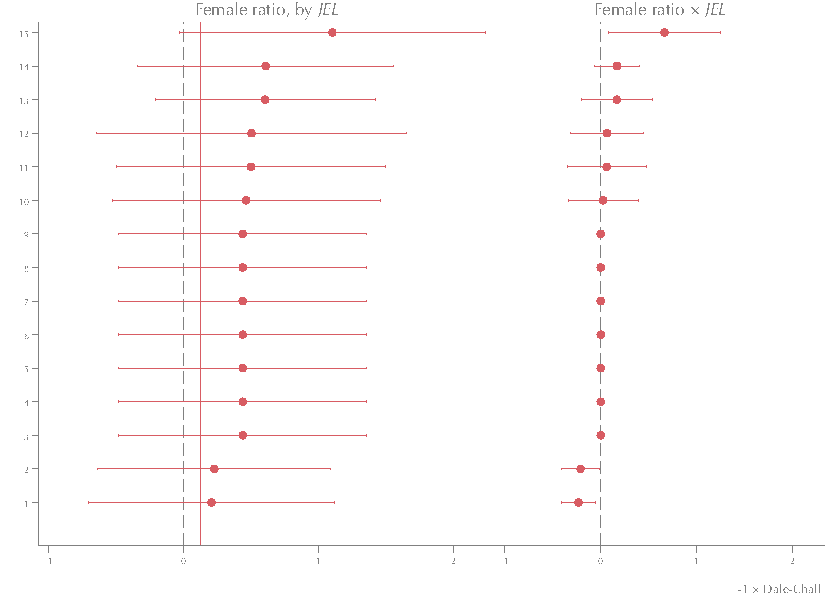
\includegraphics[width=12.3cm]{$HOME/Dropbox/Readability/draft/pdf/figure1.pdf}
		\floatfoot{
			\begin{minipage}{1.0\linewidth}
				\setlength{\belowdisplayskip}{2pt}
				\setlength{\belowdisplayshortskip}{0pt}
				\setlength{\abovedisplayskip}{2pt}
				\setlength{\abovedisplayshortskip}{0pt}
				\tiny\textit{Notes}. Sample 5,777 articles, including 561 from \textit{AER Papers \& Proceedings} (see~\autoref{footnote34}). Codes A, B, M and P dropped due to small sample sizes of female-authored papers (see~\autoref{footnote33}). Estimates from an OLS regression of:
				$$R_j=\,\beta_0+\beta_1\text{female ratio}_j + \bm\upbeta_2\,\vect J_j + \bm\upbeta_3\,\text{female ratio}_j\times\vect J_j + \bm\uptheta\,\vect X_j + \vep_j,$$
				where $R_j$ is the readability score for article $j$; $\text{female ratio}_j$ is paper $j$'s ratio of female authors to total authors; $\vect J_j$ is a $15\times1$ column vector with $k$th entry a binary variable equal to one if article $j$ is classified as the $k$th \textit{JEL} code; $\vect X_j$ is a vector of editor, journal, year, institution, English language dummies and quality controls (citation count and \(\text{max. }T_j\) fixed effects); $\vep_j$ is the error term. Left-hand graph shows marginal effects of female ratio for each \textit{JEL} code ($\beta_1+\beta_3^k$); the pink vertical line is the mean effect at observed \textit{JEL} codes (0.129, standard error 0.046). Right-hand graph displays interaction terms ($\beta_3^k$). Horizontal lines represent 90 percent confidence intervals from standard errors adjusted for clustering on editor.
			\end{minipage}
		}
	}
\end{figure}

The pink vertical line in \autoref{figure1}'s left-hand graph is the marginal effect of female authorship at the mean. Its estimate coincides with results in \autoref{table4}---women's papers require six fewer weeks of schooling to understand---and is highly significant. Points reflect marginal effects across \emph{JEL} classification; bars represent 90 percent confidence intervals from standard errors clustered by editor.

Women earn higher marks for clarity in 11 out of 15 categories; only three are at least weakly significant: Q (Agricultural and Natural Resource Economics; Environmental and Ecological Economics), N (Economic History), and J (Labour Economics). Men may be better writers in C (Mathematical and Quantitative Methods), L (Industrial Organisation), O (Economic Development, Innovation, Technological Change, and Growth) and H (Public Economics); none, however, are statistically different from zero. \autoref{figure1}'s right-hand graph displays coefficients from interacting the ratio of female co-authors with each \emph{JEL} code. Q and N are significantly above the mean, O and H significantly below it. Remaining categories are not statistically different from the mean effect.

In general, sample sizes are small and estimates imprecise---only Labour Economics and Microeconomics contain more than 100 papers written only by women (the others average 35). Nevertheless, \autoref{figure1} suggests two things. First, the mostly insignificant interaction terms indicate outlier fields are probably not driving journals' gender readability gap---nor is any specific field bucking the trend. Second, the number of women in a field appears to have little effect on the size of the gap: Agriculture\slash Environment has one of the lowest concentrations of female-authored papers---but Economic History has one of the highest (Labour Economics falls between the two). Of course, Economic History papers are still overwhelmingly---as in 74 percent---penned just by men. But given the readability gap is present in subfields with both above- and below-average rates of sole female authorship, women may need to be better writers even where more of them publish.

In the remainder of the paper, I do not explicitly control for \emph{JEL} classification (unless otherwise specified). Comparable codes are available for only a subset of the data and \autoref{table4} and \autoref{figure1} suggest they are relatively unimportant, anyway.

\section{Abstract word limits}
\label{appendixwordlimits}

I attribute the difference between NBER abstracts and published abstracts to the peer review process. However, NBER has no word limit while two journals in my sample do: \emph{Econometrica} limits abstracts to 150 words; \emph{AER} limits them to 100 words. It is therefore possible that the effects we observe are due to authors compressing the content of their abstracts rather than due to peer review.

As shown in \autoref{table6}, female-authored NBER abstracts tend to be slightly longer (more words) than male-authored abstracts---but then slightly shorter (again, in terms of total words) in published form. \autoref{figureC7a} shows the distribution of abstract lengths by gender. The graph on the left displays abstract length in NBER working papers; the graph on the right displays the distribution of abstract lengths in the published paper, again broken down by gender. Word counts in NBER drafts are more spread out; they are much more tightly compacted in the final, published version of those same papers. There appears to be no massive gender difference in the distribution of these two figures; also, there appears to be no outlier papers driving the results.

\begin{figure}
	
	\floatbox{figure}[\FBwidth]
	{
		\caption{NBER working paper release dates vis-à-vis Journal submission dates}\label{figureC7a}
	}
	{
		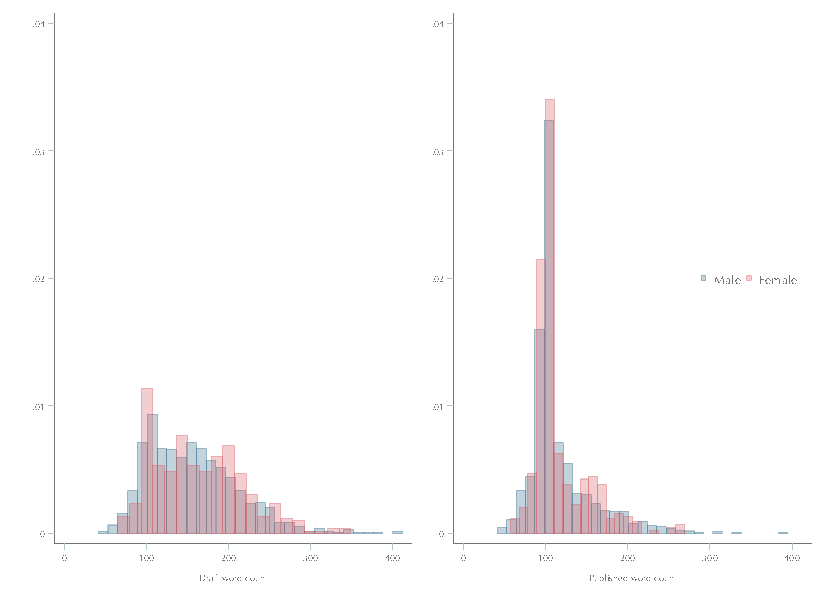
\includegraphics[width=12.3cm]{$HOME/Dropbox/Readability/draft/pdf/figureC7a.pdf}
		\floatfoot{\tiny \textit{Notes}. Distribution of abstract lengths by gender. The graph on the left displays the distribution of abstract lengths in NBER working papers; the graph on the right displays the distribution of abstract lengths in the published paper. }
	}
\end{figure}

I also repeat the analysis in \autoref{table7} but this time only on articles whose NBER abstracts fell below the official minimum word limit of the respective journal in which it was published. The subsequent analysis effectively dropped about 40 percent of the observations. Results are presented in \autoref{tableC7a}. Although standard errors are somewhat larger than those presented in \autoref{table7}, the coefficient magnitudes are very similar.

\begin{table}
    \footnotesize
    \centering
    \begin{threeparttable}
        \caption{\autoref{table7}, restricted to abstracts below journals' official word limits}
        \label{tableC7a}
        \begin{tabular}{p{4cm}S@{}S@{}S@{}S@{}S@{}}
            \toprule
            &{OLS}&\multicolumn{3}{c}{{FGLS}}&{OLS}\\\cmidrule(lr){2-2}\cmidrule(lr){3-5}\cmidrule(lr){6-6}&{\crcell[b]{Published\\[-0.1cm]article}}&{{\crcell[b]{Working\\[-0.1cm]paper}}}&{\crcell[b]{Published\\[-0.1cm]article}}&{Difference}&{\crcell[b]{Change\\[-0.1cm]in score}}\\
            \midrule
            Flesch Reading Ease           &        0.92   &        2.30   &        2.85*  &        0.55   &        0.56   \\
                                          &      (0.87)   &      (1.53)   &      (1.61)   &      (0.83)   &      (0.85)   \\
            Flesch-Kincaid                &        0.55** &        0.04   &        0.59*  &        0.54** &        0.55*  \\
                                          &      (0.26)   &      (0.35)   &      (0.33)   &      (0.27)   &      (0.28)   \\
            Gunning Fog                   &        0.57** &        0.20   &        0.73** &        0.52** &        0.53*  \\
                                          &      (0.24)   &      (0.39)   &      (0.34)   &      (0.26)   &      (0.27)   \\
            SMOG                          &        0.27*  &        0.22   &        0.45** &        0.23   &        0.24   \\
                                          &      (0.15)   &      (0.27)   &      (0.23)   &      (0.16)   &      (0.16)   \\
            Dale-Chall                    &        0.23***&        0.33***&        0.51***&        0.17** &        0.17** \\
                                          &      (0.09)   &      (0.12)   &      (0.12)   &      (0.07)   &      (0.08)   \\
            \midrule
            Editor effects                &           {\ding{51}}   &           {\ding{51}}   &           {\ding{51}}   &               &           {\ding{51}}   \\
            Journal effects               &           {\ding{51}}   &           {\ding{51}}   &           {\ding{51}}   &               &           {\ding{51}}   \\
            Year effects                  &           {\ding{51}}   &           {\ding{51}}   &           {\ding{51}}   &               &               \\
            Journal\(\times\)Year effects          &           {\ding{51}}   &           {\ding{51}}   &           {\ding{51}}   &               &           {\ding{51}}   \\
            Quality controls              &          {\(\text{\ding{51}}^2\)}   &          {\(\text{\ding{51}}^2\)}   &          {\(\text{\ding{51}}^2\)}   &               &          {\(\text{\ding{51}}^3\)}   \\
            Native speaker                &           {\ding{51}}   &           {\ding{51}}   &           {\ding{51}}   &               &           {\ding{51}}   \\
            \bottomrule
        \end{tabular}
        \begin{tablenotes}
            \tiny
            \item \textit{Notes}. Sample 1,067 NBER working papers; 1,065 published articles. Estimates are identical to those in~\autoref{table7}, except that the sample includes only articles whose NBER abstracts fell below the official minimum word limit of the respective journal in which it was published. ***, ** and * statistically significant at 1\%, 5\% and 10\%, respectively.
        \end{tablenotes}
    \end{threeparttable}
\end{table}

\clearpage

\section{Empirical consistency}
\label{seuempirical}

If topic, novelty and quality are appropriately controlled for, then discrimination is present when \autoref{Theorem1}'s three conditions hold at large enough $t$. In this section, I evaluate whether each condition holds, on average, using the entire sample of authors. In \autoref{seumatching}, I use a matching procedure to identify \autoref{Theorem1} and generate a conservative estimate of discrimination's impact on readability (\autoref{Corollary1}).

Consider first Condition 3---female-authored papers are accepted no more often than male-authored papers. The articles I evaluate have already been accepted, precluding gender analysis of acceptance rates. \autoref{seumatching} and \aref{appendixconservative} use lifetime publication counts to partially overcome this. The measure, unfortunately, embodies obvious imperfections.\footnote{\label{Footnote67}Comparing lifetime publication counts between equivalent authors accounts for most confounding factors except individual productivity---especially factors related to household responsibilities. Greater responsibility at home presumably does not affect readability (other than, perhaps, to push women's scores downward), but it may impact the number of papers women can write. As shown in \autoref{duration}, however, motherhood responsibilities after childbirth \emph{do not}, in fact, slow women down during the revision process---at least at \emph{Econometrica}.}

Luckily, gender's impact on acceptance rates has been extensively studied elsewhere. To the best of my knowledge, publication outcomes expose no female advantage anywhere, ever.  \citet{Blank1991} found that 12.7 and 10.6 percent of male- and female-authored papers were accepted at the \emph{American Economic Review} , respectively.\footnote{Women's double-blind acceptance rate was 10 percent (11 percent for men); their single-blind acceptance rate was 11.2 percent (versus 15 percent for men).} A study of \emph{JAMA}'s editorial process indicated that 44.8 percent of referees accept male-authored papers as is or if suitably revised; 29.6 percent summarily reject them. Corresponding figures for female-authored papers were 38.3 and 33.3 percent, respectively~\citep{Gilbert1994}.\footnote{The figures presented here aggregate responses in Tables 3 and 4 from  \citet[][p. 141]{Gilbert1994}. They average all individual referee recommendations, of which papers usually received several. The authors found no gender difference in final manuscript acceptance rates---although they did find that manuscripts with male corresponding authors were summarily rejected more often (41.7 percent as opposed to 37.4 percent for women).} There are also no gender differences in acceptance rates to NBER's Summer Institute programme~\citep{Chari2017}.\footnote{No gender difference was found in the pooled sample, but male-authored papers submitted to finance workshops were two percent more likely to be accepted; the effect is weakly significant. NBER's annual Summer Institute Programme is a selective three week economics conference.}  \citet{Ceci2014} provide a much more comprehensive research review on the subject. Their conclusion: ``When it comes to actual manuscripts submitted to actual journals, the evidence for gender fairness is unequivocal: there are no sex differences in acceptance rates.'' ~\citep[][p. 111]{Ceci2014}.

The data more cleanly identify Conditions 1 and 2. As their careers advance, women do write more clearly: their average readability scores are 1--5 percent higher than the readability of their first papers; their latest papers 1--7 percent higher (\aref{appendixfirstlast}). For a man, however, his average and last paper may be more poorly written than the first.

\begin{figure}
	
	\floatbox{figure}[\FBwidth]
	{
		\caption{Readability of authors' $t$th publication}\label{figure3}
	}
	{
		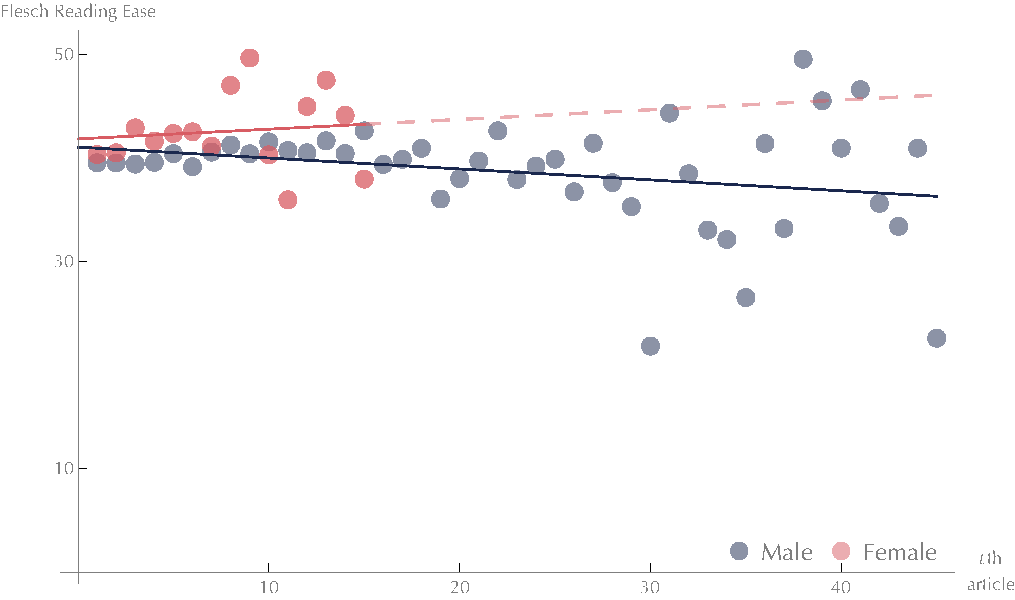
\includegraphics[width=12.3cm]{$HOME/Dropbox/Readability/draft/pdf/figure3.pdf}
		\floatfoot{\tiny \textit{Notes}. Mean Flesch Reading Ease scores grouped by authors' first, second, \ldots, $t$th, \ldots~publication in the data. Lines of best fit are estimated separately for men and women on the grouped averages using OLS. Dotted line indicates out-of-sample forecast (the largest $t$ for a woman is 15; for a man it's 45).}
	}
\end{figure}

\autoref{figure3} plots mean Flesch Reading Ease scores grouped by authors' $t\text{th}$ article; as the count increases, men and women diverge.\footnote{In an earlier version of this paper, I estimated the mean additional contribution each paper makes to an author's readability ~\citep[][pp. 23--24]{Hengel2016}. This analysis included the full set of controls used in \autoref{authorlevel}. The results and conclusions were similar to those presented here.}\autoref{table8} tests significance of that divergence by FGLS estimation of \autoref{equation1} (omitting $R_{it-1}$) on subsamples corresponding to authors' first ($t=1$), second ($t=2$), third ($t=3$), fourth and fifth ($t=4\text{--}5$) and sixth and up ($t\ge6$) articles published in the journals and time periods covered by the data. Only marginal effects on co-authoring with women for female authors are shown ($\beta_1$). Final column is a population-averaged estimate on the pooled sample. Regressions in columns ($t=1$) to ($t\ge6$) are weighted by $1/N_j$ (see \autoref{authorlevel}), standard errors adjusted for two-way clustering on editor and author and corrected for cross-model correlation. Final column estimates are unweighted, error correlations are specified by an auto-regressive process of order one and standard errors are clustered on author.

All figures agree---women write better---but the magnitude and significance of that difference increases as $t$ increases.\footnote{See [][AppendixEqualityTests] for coefficient equality test statistics.} Between columns ($t=1$) and ($t=2$), the gap marginally widens but is not significant; after that, it triples (at least); the increase is significant ($p<0.05$) for all five scores.\footnote{Figures in columns ($t=2$) and ($t=3$) of \autoref{table8} are roughly in line with third column estimates in \autoref{table7}---on average, $t=2.7$ for female-authored articles released first as NBER working papers.} At higher publication counts, estimates are somewhat smaller than column ($t=3$)---but still larger than columns ($t=1$) and ($t=2$)---although figures are only weakly significant and suffer from very small samples of female authors.\footnote{Only 40 female authors have 4--5 publications in the data; 28 have six or more. (512 men have 4--5 publications; 545 have more than that.)}

\begin{table}
    \footnotesize
    \centering
    \begin{threeparttable}
        \caption{Gender gap in readability at increasing \(t\)}
        \label{table8}
        \begin{tabular}{p{3cm}S@{}S@{}S@{}S@{}S@{}S@{}S@{}}
            \toprule
            &{\(t=1\)}&{\(t=2\)}&{\(t=3\)}&{\(t=4\text{--}5\)}&{\(t\ge6\)}&{All}\\
            \midrule
            Flesch Reading Ease           &        0.24   &        1.56*  &        4.71***&        2.73   &        3.35   &        1.65** \\
                                          &      (0.63)   &      (0.91)   &      (1.13)   &      (1.97)   &      (2.14)   &      (0.72)   \\
            Flesch-Kincaid                &        0.07   &        0.17   &        0.83***&        0.58   &        0.62   &        0.21   \\
                                          &      (0.14)   &      (0.21)   &      (0.25)   &      (0.41)   &      (0.44)   &      (0.15)   \\
            Gunning Fog                   &        0.20   &        0.38   &        1.11***&        0.83*  &        0.88   &        0.43** \\
                                          &      (0.16)   &      (0.25)   &      (0.30)   &      (0.47)   &      (0.54)   &      (0.18)   \\
            SMOG                          &        0.11   &        0.26   &        0.74***&        0.64*  &        0.66*  &        0.33** \\
                                          &      (0.12)   &      (0.17)   &      (0.21)   &      (0.37)   &      (0.38)   &      (0.13)   \\
            Dale-Chall                    &        0.07   &        0.10   &        0.34***&        0.29*  &        0.43*  &        0.17** \\
                                          &      (0.06)   &      (0.08)   &      (0.12)   &      (0.17)   &      (0.24)   &      (0.07)   \\
            \midrule
            No. observations              &       6,876   &       2,827   &       1,674   &       1,908   &       2,777   &      12,013   \\
            \(N_j\)                       &           {\ding{51}}   &           {\ding{51}}   &           {\ding{51}}   &           {\ding{51}}   &           {\ding{51}}   &           {\ding{51}}   \\
            Editor effects                &           {\ding{51}}   &           {\ding{51}}   &           {\ding{51}}   &           {\ding{51}}   &           {\ding{51}}   &           {\ding{51}}   \\
            Journal effects               &           {\ding{51}}   &           {\ding{51}}   &           {\ding{51}}   &           {\ding{51}}   &           {\ding{51}}   &           {\ding{51}}   \\
            Year effects                  &           {\ding{51}}   &           {\ding{51}}   &           {\ding{51}}   &           {\ding{51}}   &           {\ding{51}}   &           {\ding{51}}   \\
            Journal\(\times\)Year effects          &               &               &               &               &               &           {\ding{51}}   \\
            Institution effects           &           {\ding{51}}   &           {\ding{51}}   &           {\ding{51}}   &           {\ding{51}}   &           {\ding{51}}   &           {\ding{51}}   \\
            Quality controls              &          {\(\text{\ding{51}}^4\)}   &          {\(\text{\ding{51}}^4\)}   &          {\(\text{\ding{51}}^4\)}   &          {\(\text{\ding{51}}^4\)}   &          {\(\text{\ding{51}}^4\)}   &          {\(\text{\ding{51}}^1\)}   \\
            Native speaker                &           {\ding{51}}   &           {\ding{51}}   &           {\ding{51}}   &           {\ding{51}}   &           {\ding{51}}   &           {\ding{51}}   \\
            \bottomrule
        \end{tabular}
        \begin{tablenotes}
            \tiny
            \item \textit{Notes}. \(\beta_1\) from FGLS estimation of~\autoref{equation1} without lagged dependent variable. First column restricts sample to authors' first publication in the data (\(t=1\)), second column to their second (\(t=2\)), \textit{etc.} Regressions weighted by \(1/N_j\) (see~\autoref{authorlevel}). Standard errors (in parentheses) adjusted for two-way clustering (editor and author) and cross-model correlation. Final column estimates from an unweighted population-averaged regression; error correlations specified by an auto-regressive process of order one and standard errors (in parentheses) adjusted for one-way clustering on author. Quality controls denoted by \(\text{\ding{51}}^1\) include citation count and \(\text{max. }T_j\) fixed effects; \(\text{\ding{51}}^4\) includes citation count, only. ***, ** and * statistically significant at 1\%, 5\% and 10\%, respectively.
        \end{tablenotes}
    \end{threeparttable}
\end{table}

First-time publications are not driving the observed readability gap. \autoref{figure3} suggests little or no gender difference when $t=1$; \autoref{table8} backs this up. Coefficients in column ($t=1$) are imprecise, roughly half the size of those from a pooled regression (last column) and a fraction the size of estimates in columns ($t=3$), ($t=4\text{--}5$) and ($t\ge6$). [Wald tests][AppendixEqualityTests] reject equality of $\beta_1$ in the first and third models at $p<0.01$ for the Flesch Reading Ease, Flesch-Kincaid and SMOG scores and $p<0.05$ for the Gunning Fog and Dale-Chall scores.

\autoref{tableC6} displays $\chi^2$ test statistics from Wald tests of $\beta_1$ (\autoref{equation1}) equality across estimation results in \autoref{table8}. 

\begin{table}[H]
    \footnotesize
    \centering
    \begin{threeparttable}
        \caption{\autoref{table8}, equality test statistics}
        \label{tableC6}
        \sisetup{round-precision=3}
        \begin{tabular}{p{3cm}S@{}S@{}S@{}S@{}S@{}S@{}}
            \toprule
            &{\(t=1\) vs. 2}&{\(t=1\) vs. 3}&{\(t=1\) vs. 4--5}&{\(t=1\) vs. \(\ge6\)}&{\(t=2\) vs. 3}\\
            \midrule
            Flesch Reading Ease &       0.570&       4.571&       0.100&       0.093&       1.010\\
            Flesch-Kincaid      &       0.040&       1.061&       0.227&       0.897&       0.279\\
            Gunning Fog         &       0.042&       0.179&       0.144&       1.061&       0.018\\
            SMOG                &       0.196&       0.373&       0.659&       0.420&       0.014\\
            Dale-Chall          &       2.825&       1.117&       0.019&       0.106&       4.054\\
            \bottomrule
        \end{tabular}
        \begin{tablenotes}
            \tiny
            \item \textit{Notes}. \(\chi^2\) test statistics from Wald tests of \(\beta_1\) (\autoref{equation1}) equality across estimation results in~\autoref{table8}.
        \end{tablenotes}
    \end{threeparttable}
\end{table}

\clearpage

\section{Readability meta-analysis}
\label{appendixmetaanalysis}

\section{Alternative measures of an article's ``gender''}
\label{appendixalternativemeasure}

The following tables repeat the principal analyses from the paper using several alternative measures of of an article's ``gender''.

\subsection{Majority female-authored}
\label{appendixmajoirty}

In the following tables, article gender is represented by a binary variable equal to one if at least half of all authors are female; articles below that threshold with at least one female author are excluded.

\begin{table}[H]
    \footnotesize
    \centering
    \begin{threeparttable}
        \caption{\autoref{table4}, 50\% or more female-authored}
        \label{tableC4c}
        \begin{tabular}{p{2.64cm}S@{}S@{}S@{}S@{}S@{}S@{}S@{}}
            \toprule
            &{(1)}&{(2)}&{(3)}&{(4)}&{(5)}&{(6)}&{(7)}\\
            \midrule
            \mrow{3cm}{Flesch Reading Ease}&        0.91***&        0.89***&        0.87** &        0.83** &        0.93***&        0.64*  &        1.05** \\
                                          &      (0.32)   &      (0.32)   &      (0.33)   &      (0.33)   &      (0.34)   &      (0.37)   &      (0.46)   \\
            \mrow{3cm}{Flesch-Kincaid}    &        0.16*  &        0.16*  &        0.16*  &        0.16*  &        0.18** &        0.18*  &        0.23** \\
                                          &      (0.08)   &      (0.08)   &      (0.08)   &      (0.08)   &      (0.09)   &      (0.09)   &      (0.10)   \\
            \mrow{3cm}{Gunning Fog}       &        0.27***&        0.26***&        0.27***&        0.26***&        0.28***&        0.29** &        0.32***\\
                                          &      (0.09)   &      (0.10)   &      (0.10)   &      (0.10)   &      (0.10)   &      (0.11)   &      (0.12)   \\
            \mrow{3cm}{SMOG}              &        0.17** &        0.17** &        0.17** &        0.16** &        0.18** &        0.17** &        0.21** \\
                                          &      (0.07)   &      (0.07)   &      (0.07)   &      (0.07)   &      (0.07)   &      (0.08)   &      (0.09)   \\
            \mrow{3cm}{Dale-Chall}        &        0.09** &        0.08** &        0.08** &        0.08** &        0.09** &        0.07*  &        0.10*  \\
                                          &      (0.03)   &      (0.03)   &      (0.04)   &      (0.04)   &      (0.04)   &      (0.04)   &      (0.05)   \\
            \midrule
            Editor effects                &           {\ding{51}}   &           {\ding{51}}   &           {\ding{51}}   &           {\ding{51}}   &           {\ding{51}}   &           {\ding{51}}   &           {\ding{51}}   \\
            Journal effects               &           {\ding{51}}   &           {\ding{51}}   &           {\ding{51}}   &           {\ding{51}}   &           {\ding{51}}   &           {\ding{51}}   &           {\ding{51}}   \\
            Year effects                  &               &           {\ding{51}}   &           {\ding{51}}   &           {\ding{51}}   &           {\ding{51}}   &           {\ding{51}}   &           {\ding{51}}   \\
            Journal\(\times\)Year effects          &               &               &           {\ding{51}}   &           {\ding{51}}   &           {\ding{51}}   &           {\ding{51}}   &           {\ding{51}}   \\
            Institution effects           &               &               &               &           {\ding{51}}   &           {\ding{51}}   &           {\ding{51}}   &           {\ding{51}}   \\
            Quality controls              &               &               &               &               &          {\(\text{\ding{51}}^1\)}   &          {\(\text{\ding{51}}^1\)}   &          {\(\text{\ding{51}}^1\)}   \\
            Native speaker                &               &               &               &               &           {\ding{51}}   &           {\ding{51}}   &           {\ding{51}}   \\
            \textit{JEL} (primary) effects&               &               &               &               &               &           {\ding{51}}   &               \\
            \textit{JEL} (tertiary) effects&               &               &               &               &               &               &           {\ding{51}}   \\
            \bottomrule
        \end{tabular}
        \begin{tablenotes}
            \tiny
            \item \textit{Notes}. 8,803 articles in (1)--(5); 4,917 articles in (6); 5,282 articles---including 383 from \textit{AER Papers \& Proceedings} (see~\autoref{footnote34})---in (7). Figures represent the coefficient on a binary variable equal to 1 for papers with 50 percent (or more) female authors. Papers with less than half but more than one female author are excluded. Quality controls denoted by \(\text{\ding{51}}^1\) include citation count and \(\text{max. }T_j\) fixed effects. Standard errors clustered on editor in parentheses. ***, ** and * statistically significant at 1\%, 5\% and 10\%, respectively.
        \end{tablenotes}
    \end{threeparttable}
\end{table}

\begin{table}
    \footnotesize
    \centering
    \begin{threeparttable}
        \caption{\autoref{table5}, papers with 50\% or more female authors}
        \label{tableC5b}
        \begin{tabular}{p{4cm}S@{}S@{}S@{}S@{}S@{}}
            \toprule
            &{\crcell[b]{Flesch\\[-0.1cm]Reading\\[-0.1cm]Ease}}&{\crcell[b]{Flesch-\\[-0.1cm] Kincaid}}&{\crcell[b]{Gunning\\[-0.1cm]Fog}}&{SMOG}&{\crcell[b]{Dale-\\[-0.1cm]Chall}}\\
            \midrule
            \mrow{4cm}{Female-authored (women)}&        1.82** &        0.34***&        0.47***&        0.30** &        0.13*  \\
                                          &      (0.69)   &      (0.13)   &      (0.17)   &      (0.13)   &      (0.08)   \\
            \mrow{4cm}{Female-authored (men)}&        0.58   &        0.09   &        0.11   &        0.04   &        0.05   \\
                                          &      (0.65)   &      (0.13)   &      (0.17)   &      (0.12)   &      (0.05)   \\
            \mrow{4cm}{Female-authored\(\times\)male}&       -1.23   &       -0.25   &       -0.35   &       -0.26   &       -0.08   \\
                                          &      (0.89)   &      (0.17)   &      (0.22)   &      (0.16)   &      (0.08)   \\
            \mrow{4cm}{Lagged score}      &        0.03*  &        0.04** &        0.03   &        0.02   &        0.02   \\
                                          &      (0.02)   &      (0.02)   &      (0.02)   &      (0.02)   &      (0.02)   \\
            \mcol{\rule{0pt}{4ex}\textit{\(z\)-test for no serial correlation}} \\
            Order 1&      -18.43   &      -14.71   &      -15.72   &      -18.43   &      -18.18   \\
            Order 2                       &        0.31   &        0.16   &        0.37   &        0.39   &       -0.88   \\
            \midrule
            \(N_j\)              &           {\ding{51}}   &           {\ding{51}}   &           {\ding{51}}   &           {\ding{51}}   &           {\ding{51}}   \\
            Editor effects                &           {\ding{51}}   &           {\ding{51}}   &           {\ding{51}}   &           {\ding{51}}   &           {\ding{51}}   \\
            Journal effects               &           {\ding{51}}   &           {\ding{51}}   &           {\ding{51}}   &           {\ding{51}}   &           {\ding{51}}   \\
            Year effects                  &           {\ding{51}}   &           {\ding{51}}   &           {\ding{51}}   &           {\ding{51}}   &           {\ding{51}}   \\
            Journal\(\times\)Year effects          &           {\ding{51}}   &           {\ding{51}}   &           {\ding{51}}   &           {\ding{51}}   &           {\ding{51}}   \\
            Institution effects           &           {\ding{51}}   &           {\ding{51}}   &           {\ding{51}}   &           {\ding{51}}   &           {\ding{51}}   \\
            Quality controls              &          {\(\text{\ding{51}}^1\)}   &          {\(\text{\ding{51}}^1\)}   &          {\(\text{\ding{51}}^1\)}   &          {\(\text{\ding{51}}^1\)}   &          {\(\text{\ding{51}}^1\)}   \\
            Native speaker                &           {\ding{51}}   &           {\ding{51}}   &           {\ding{51}}   &           {\ding{51}}   &           {\ding{51}}   \\
            \bottomrule
        \end{tabular}
        \begin{tablenotes}
            \tiny
            \item \textit{Notes}. Sample 8,593 observations (2,723 authors). ***, ** and * statistically significant at 1\%, 5\% and 10\%, respectively.
        \end{tablenotes}
    \end{threeparttable}
\end{table}

\begin{table}[H]
    \footnotesize
    \centering
    \begin{threeparttable}
        \caption{\autoref{table8}, papers authored at least 50\% by women}
        \label{table8XB}
        \begin{tabular}{p{3cm}S@{}S@{}S@{}S@{}S@{}S@{}S@{}}
            \toprule
            &{\(t=1\)}&{\(t=2\)}&{\(t=3\)}&{\(t=4\text{--}5\)}&{\(t\ge6\)}&{All}\\
            \midrule
            Flesch Reading Ease           &        0.44   &        1.39** &        3.39***&        1.67   &        2.91** &        1.80***\\
                                          &      (0.47)   &      (0.66)   &      (1.02)   &      (1.34)   &      (1.38)   &      (0.63)   \\
            Flesch-Kincaid                &        0.07   &        0.17   &        0.66***&        0.46*  &        0.49   &        0.29** \\
                                          &      (0.12)   &      (0.16)   &      (0.19)   &      (0.24)   &      (0.34)   &      (0.13)   \\
            Gunning Fog                   &        0.19   &        0.29   &        0.83***&        0.57** &        0.63   &        0.42** \\
                                          &      (0.13)   &      (0.19)   &      (0.23)   &      (0.29)   &      (0.41)   &      (0.16)   \\
            SMOG                          &        0.12   &        0.20   &        0.51***&        0.40*  &        0.46   &        0.28** \\
                                          &      (0.09)   &      (0.13)   &      (0.17)   &      (0.22)   &      (0.29)   &      (0.12)   \\
            Dale-Chall                    &        0.08*  &        0.06   &        0.18   &        0.16   &        0.30   &        0.15** \\
                                          &      (0.05)   &      (0.06)   &      (0.12)   &      (0.12)   &      (0.19)   &      (0.06)   \\
            \midrule
            No. observations              &       6,402   &       2,679   &       1,556   &       1,778   &       2,580   &       9,590   \\
            \(N_j\)                       &           {\ding{51}}   &           {\ding{51}}   &           {\ding{51}}   &           {\ding{51}}   &           {\ding{51}}   &           {\ding{51}}   \\
            Editor effects                &           {\ding{51}}   &           {\ding{51}}   &           {\ding{51}}   &           {\ding{51}}   &           {\ding{51}}   &           {\ding{51}}   \\
            Journal effects               &           {\ding{51}}   &           {\ding{51}}   &           {\ding{51}}   &           {\ding{51}}   &           {\ding{51}}   &           {\ding{51}}   \\
            Year effects                  &           {\ding{51}}   &           {\ding{51}}   &           {\ding{51}}   &           {\ding{51}}   &           {\ding{51}}   &           {\ding{51}}   \\
            Journal\(\times\)Year effects          &               &               &               &               &               &           {\ding{51}}   \\
            Institution effects           &           {\ding{51}}   &           {\ding{51}}   &           {\ding{51}}   &           {\ding{51}}   &           {\ding{51}}   &           {\ding{51}}   \\
            Quality controls              &          {\(\text{\ding{51}}^4\)}   &          {\(\text{\ding{51}}^4\)}   &          {\(\text{\ding{51}}^4\)}   &          {\(\text{\ding{51}}^4\)}   &          {\(\text{\ding{51}}^4\)}   &          {\(\text{\ding{51}}^1\)}   \\
            Native speaker                &           {\ding{51}}   &           {\ding{51}}   &           {\ding{51}}   &           {\ding{51}}   &           {\ding{51}}   &           {\ding{51}}   \\
            \bottomrule
        \end{tabular}
        \begin{tablenotes}
            \tiny
            \item \textit{Notes}. Columns display estimates identical to those in Table 7, except that female ratio has been replaced with a dummy variable equal to 1 if a weak majority (50\% or more) of authors are female. ***, ** and * statistically significant at 1\%, 5\% and 10\%, respectively.
        \end{tablenotes}
    \end{threeparttable}
\end{table}

\begin{table}[H]
    \begin{adjustwidth}{-0.085cm}{}
    \footnotesize
    \centering
    \begin{threeparttable}
        \caption{\autoref{table11}, papers with at least 50\% female authors}
        \label{table11XC}
        \sisetup{round-precision=3,table-format=3.4}
        \begin{tabular}{p{2.64cm}SSSSSSS}
            \toprule
            &{(1)}&{(2)}&{(3)}&{(4)}&{(5)}&{(6)}&{(7)}\\
            \midrule
            Fem50                         &       3.548***&       3.892***&       3.890***&       3.565***&       3.897***&       5.419***&       5.506***\\
                                          &     (1.243)   &     (1.238)   &     (1.230)   &     (1.218)   &     (1.232)   &     (1.452)   &     (1.495)   \\
            Max. \(t_j\)                  &      -0.208***&      -0.216***&      -0.210***&      -0.208***&      -0.209***&      -0.222** &      -0.213** \\
                                          &     (0.071)   &     (0.072)   &     (0.071)   &     (0.071)   &     (0.072)   &     (0.090)   &     (0.087)   \\
            No. pages                     &       0.186***&       0.186***&       0.185***&       0.186***&       0.185***&       0.225***&       0.214***\\
                                          &     (0.026)   &     (0.026)   &     (0.026)   &     (0.026)   &     (0.026)   &     (0.041)   &     (0.044)   \\
            \(N\)                         &       1.072** &       1.062** &       1.049** &       1.071** &       1.056** &       1.324** &       1.208*  \\
                                          &     (0.426)   &     (0.423)   &     (0.425)   &     (0.426)   &     (0.424)   &     (0.626)   &     (0.634)   \\
            Order                         &       0.211** &       0.211** &       0.209** &       0.211** &       0.209** &       0.513** &       0.493** \\
                                          &     (0.092)   &     (0.092)   &     (0.092)   &     (0.092)   &     (0.092)   &     (0.233)   &     (0.226)   \\
            No. citations                 &       0.000   &       0.000   &       0.000   &       0.000   &       0.000   &      -0.003** &      -0.003** \\
                                          &     (0.000)   &     (0.000)   &     (0.000)   &     (0.000)   &     (0.000)   &     (0.001)   &     (0.001)   \\
            Mother                        &               &               &      -3.395   &               &      -7.515** &     -14.417***&     -14.584***\\
                                          &               &               &     (2.449)   &               &     (3.037)   &     (4.161)   &     (3.877)   \\
            Birth                         &               &               &               &      -0.284   &       6.878   &      12.705*  &      13.160** \\
                                          &               &               &               &     (3.328)   &     (4.469)   &     (6.396)   &     (6.310)   \\
            Constant                      &      37.471***&      37.300***&      37.478***&      37.467***&      37.572***&      14.543***&      15.423***\\
                                          &     (2.098)   &     (2.141)   &     (2.105)   &     (2.108)   &     (2.116)   &     (2.997)   &     (2.849)   \\
            \midrule
            Editor effects                &           {\ding{51}}   &           {\ding{51}}   &           {\ding{51}}   &           {\ding{51}}   &           {\ding{51}}   &           {\ding{51}}   &           {\ding{51}}   \\
            Year effects                  &           {\ding{51}}   &           {\ding{51}}   &           {\ding{51}}   &           {\ding{51}}   &           {\ding{51}}   &           {\ding{51}}   &           {\ding{51}}   \\
            Institution effects           &           {\ding{51}}   &           {\ding{51}}   &           {\ding{51}}   &           {\ding{51}}   &           {\ding{51}}   &           {\ding{51}}   &           {\ding{51}}   \\
            \textit{JEL} (primary) effects&               &               &               &               &               &               &           {\ding{51}}   \\
            No. observations              &       2,547   &       2,532   &       2,547   &       2,547   &       2,547   &       1,214   &       1,214   \\
            \bottomrule
        \end{tabular}
        \begin{tablenotes}
            \tiny
            \item \textit{Notes}. Sample 2,626 articles. Columns display estimates identical to those in~\autoref{table11}, except that female ratio has been replaced with a dummy variable equal to 1 if a weak majority (50% or more) of authors are female. (Papers with a minority—but positive—number of female authors are excluded.) ***, ** and * statistically significant at 1\%, 5\% and 10\%, respectively.
        \end{tablenotes}
    \end{threeparttable}
    \end{adjustwidth}
\end{table}

\begin{table}[H]
    \footnotesize
    \centering
    \begin{threeparttable}
        \caption{\autoref{table7}, papers with more than 50\% female authors}
        \label{tableXC}
        \begin{tabular}{p{4cm}S@{}S@{}S@{}S@{}S@{}}
            \toprule
            &{OLS}&\multicolumn{3}{c}{{FGLS}}&{OLS}\\\cmidrule(lr){2-2}\cmidrule(lr){3-5}\cmidrule(lr){6-6}&{\crcell[b]{Published\\[-0.1cm]article}}&{{\crcell[b]{Working\\[-0.1cm]paper}}}&{\crcell[b]{Published\\[-0.1cm]article}}&{Difference}&{\crcell[b]{Change\\[-0.1cm]in score}}\\
            \midrule
            Flesch Reading Ease           &        1.32***&        1.40** &        2.48***&        1.08***&        1.07***\\
                                          &      (0.44)   &      (0.69)   &      (0.73)   &      (0.41)   &      (0.41)   \\
            Flesch-Kincaid                &        0.43***&        0.17   &        0.56***&        0.39***&        0.39***\\
                                          &      (0.15)   &      (0.17)   &      (0.16)   &      (0.12)   &      (0.12)   \\
            Gunning Fog                   &        0.45***&        0.24   &        0.63***&        0.39***&        0.39***\\
                                          &      (0.17)   &      (0.18)   &      (0.18)   &      (0.13)   &      (0.13)   \\
            SMOG                          &        0.28** &        0.16   &        0.40***&        0.24***&        0.24***\\
                                          &      (0.11)   &      (0.11)   &      (0.12)   &      (0.09)   &      (0.09)   \\
            Dale-Chall                    &        0.14***&        0.17***&        0.28***&        0.12***&        0.11***\\
                                          &      (0.03)   &      (0.05)   &      (0.06)   &      (0.03)   &      (0.03)   \\
            \midrule
            Editor effects                &           {\ding{51}}   &           {\ding{51}}   &           {\ding{51}}   &               &           {\ding{51}}   \\
            Journal effects               &           {\ding{51}}   &           {\ding{51}}   &           {\ding{51}}   &               &           {\ding{51}}   \\
            Year effects                  &           {\ding{51}}   &           {\ding{51}}   &           {\ding{51}}   &               &               \\
            Journal\(\times\)Year effects          &           {\ding{51}}   &           {\ding{51}}   &           {\ding{51}}   &               &           {\ding{51}}   \\
            Quality controls              &          {\(\text{\ding{51}}^2\)}   &          {\(\text{\ding{51}}^2\)}   &          {\(\text{\ding{51}}^2\)}   &               &          {\(\text{\ding{51}}^3\)}   \\
            Native speaker                &           {\ding{51}}   &           {\ding{51}}   &           {\ding{51}}   &               &           {\ding{51}}   \\
            \bottomrule
        \end{tabular}
        \begin{tablenotes}
            \tiny
            \item \textit{Notes}. Sample 1,566 NBER working papers; 1,564 published articles (235 female-authored). Estimates exclude 273 pre-internet double-blind reviewed articles (see~\autoref{Footnote51}). Columns display estimates identical to those in~\autoref{table7}, except that female ratio has been replaced with a dummy variable equal to 1 if a weak majority (50\% or more) of authors are female. (Papers with a minority---but positive---number of female authors are excluded.) ***, ** and * statistically significant at 1\%, 5\% and 10\%, respectively.
        \end{tablenotes}
    \end{threeparttable}
\end{table}

\clearpage

\subsection{At least one female author}
\label{appendixminority}

In the following tables, papers authored entirely by women are compared to papers authored entirely by men.

\begin{table}
    \footnotesize
    \centering
    \begin{threeparttable}
        \caption{\autoref{table4}, papers with at least one female author}
        \label{tableC4b}
        \begin{tabular}{p{2.64cm}S@{}S@{}S@{}S@{}S@{}S@{}S@{}}
            \toprule
            &{(1)}&{(2)}&{(3)}&{(4)}&{(5)}&{(6)}&{(7)}\\
            \midrule
            \mrow{3cm}{Flesch Reading Ease}&        0.49   &        0.48   &        0.47   &        0.42   &        0.51   &        0.14   &        0.17   \\
                                          &      (0.38)   &      (0.38)   &      (0.39)   &      (0.38)   &      (0.38)   &      (0.42)   &      (0.45)   \\
            \mrow{3cm}{Flesch-Kincaid}    &        0.11   &        0.11   &        0.11   &        0.11   &        0.12   &        0.08   &        0.06   \\
                                          &      (0.07)   &      (0.08)   &      (0.08)   &      (0.08)   &      (0.08)   &      (0.09)   &      (0.09)   \\
            \mrow{3cm}{Gunning Fog}       &        0.20** &        0.20** &        0.20** &        0.20** &        0.20** &        0.16   &        0.09   \\
                                          &      (0.09)   &      (0.09)   &      (0.09)   &      (0.09)   &      (0.10)   &      (0.11)   &      (0.11)   \\
            \mrow{3cm}{SMOG}              &        0.12*  &        0.12*  &        0.13*  &        0.12*  &        0.12*  &        0.08   &        0.05   \\
                                          &      (0.07)   &      (0.07)   &      (0.07)   &      (0.07)   &      (0.07)   &      (0.08)   &      (0.08)   \\
            \mrow{3cm}{Dale-Chall}        &        0.07** &        0.07** &        0.07** &        0.06*  &        0.07** &        0.06   &        0.04   \\
                                          &      (0.03)   &      (0.03)   &      (0.03)   &      (0.03)   &      (0.03)   &      (0.04)   &      (0.04)   \\
            \midrule
            Editor effects                &           {\ding{51}}   &           {\ding{51}}   &           {\ding{51}}   &           {\ding{51}}   &           {\ding{51}}   &           {\ding{51}}   &           {\ding{51}}   \\
            Journal effects               &           {\ding{51}}   &           {\ding{51}}   &           {\ding{51}}   &           {\ding{51}}   &           {\ding{51}}   &           {\ding{51}}   &           {\ding{51}}   \\
            Year effects                  &               &           {\ding{51}}   &           {\ding{51}}   &           {\ding{51}}   &           {\ding{51}}   &           {\ding{51}}   &           {\ding{51}}   \\
            Journal\(\times\)Year effects          &               &               &           {\ding{51}}   &           {\ding{51}}   &           {\ding{51}}   &           {\ding{51}}   &           {\ding{51}}   \\
            Institution effects           &               &               &               &           {\ding{51}}   &           {\ding{51}}   &           {\ding{51}}   &           {\ding{51}}   \\
            Quality controls              &               &               &               &               &          {\(\text{\ding{51}}^1\)}   &          {\(\text{\ding{51}}^1\)}   &          {\(\text{\ding{51}}^1\)}   \\
            Native speaker                &               &               &               &               &           {\ding{51}}   &           {\ding{51}}   &           {\ding{51}}   \\
            \textit{JEL} (primary) effects&               &               &               &               &               &           {\ding{51}}   &               \\
            \textit{JEL} (tertiary) effects&               &               &               &               &               &               &           {\ding{51}}   \\
            \bottomrule
        \end{tabular}
        \begin{tablenotes}
            \tiny
            \item \textit{Notes}. 9,121 articles in (1)--(5); 5,216 articles in (6); 5,659 articles---including 383 from \textit{AER Papers \& Proceedings} (see~\autoref{footnote34})---in (7). Figures represent the coefficient on a binary variable equal to 1 for papers with at least one female author. Quality controls denoted by \(\text{\ding{51}}^1\) include citation count and \(\text{max. }T_j\) fixed effects. Standard errors clustered on editor in parentheses. ***, ** and * statistically significant at 1\%, 5\% and 10\%, respectively.
        \end{tablenotes}
    \end{threeparttable}
\end{table}

\begin{table}
    \footnotesize
    \centering
    \begin{threeparttable}
        \caption{\autoref{table8}, papers with at least one female author}
        \label{table8XA}
        \begin{tabular}{p{3cm}S@{}S@{}S@{}S@{}S@{}S@{}S@{}}
            \toprule
            &{\(t=1\)}&{\(t=2\)}&{\(t=3\)}&{\(t=4\text{--}5\)}&{\(t\ge6\)}&{All}\\
            \midrule
            Flesch Reading Ease           &        0.23   &        0.59   &        3.21***&        1.67   &        1.63   &        0.81   \\
                                          &      (0.40)   &      (0.64)   &      (0.80)   &      (1.16)   &      (1.49)   &      (0.54)   \\
            Flesch-Kincaid                &        0.06   &       -0.03   &        0.56***&        0.48** &        0.33   &        0.09   \\
                                          &      (0.09)   &      (0.17)   &      (0.15)   &      (0.23)   &      (0.35)   &      (0.11)   \\
            Gunning Fog                   &        0.16   &        0.08   &        0.68***&        0.58*  &        0.44   &        0.20   \\
                                          &      (0.11)   &      (0.18)   &      (0.19)   &      (0.29)   &      (0.42)   &      (0.14)   \\
            SMOG                          &        0.10   &        0.06   &        0.44***&        0.40*  &        0.35   &        0.16   \\
                                          &      (0.08)   &      (0.12)   &      (0.14)   &      (0.22)   &      (0.29)   &      (0.10)   \\
            Dale-Chall                    &        0.08** &        0.03   &        0.23***&        0.15   &        0.18   &        0.09*  \\
                                          &      (0.04)   &      (0.06)   &      (0.08)   &      (0.10)   &      (0.16)   &      (0.05)   \\
            \midrule
            No. observations              &       6,876   &       2,827   &       1,674   &       1,908   &       2,777   &      12,013   \\
            \(N_j\)                       &           {\ding{51}}   &           {\ding{51}}   &           {\ding{51}}   &           {\ding{51}}   &           {\ding{51}}   &           {\ding{51}}   \\
            Editor effects                &           {\ding{51}}   &           {\ding{51}}   &           {\ding{51}}   &           {\ding{51}}   &           {\ding{51}}   &           {\ding{51}}   \\
            Journal effects               &           {\ding{51}}   &           {\ding{51}}   &           {\ding{51}}   &           {\ding{51}}   &           {\ding{51}}   &           {\ding{51}}   \\
            Year effects                  &           {\ding{51}}   &           {\ding{51}}   &           {\ding{51}}   &           {\ding{51}}   &           {\ding{51}}   &           {\ding{51}}   \\
            Journal\(\times\)Year effects          &               &               &               &               &               &           {\ding{51}}   \\
            Institution effects           &           {\ding{51}}   &           {\ding{51}}   &           {\ding{51}}   &           {\ding{51}}   &           {\ding{51}}   &           {\ding{51}}   \\
            Quality controls              &          {\(\text{\ding{51}}^4\)}   &          {\(\text{\ding{51}}^4\)}   &          {\(\text{\ding{51}}^4\)}   &          {\(\text{\ding{51}}^4\)}   &          {\(\text{\ding{51}}^4\)}   &          {\(\text{\ding{51}}^1\)}   \\
            Native speaker                &           {\ding{51}}   &           {\ding{51}}   &           {\ding{51}}   &           {\ding{51}}   &           {\ding{51}}   &           {\ding{51}}   \\
            \bottomrule
        \end{tabular}
        \begin{tablenotes}
            \tiny
            \item \textit{Notes}. Columns display estimates identical to those in Table 7, except that female ratio has been replaced with a dummy variable equal to 1 if at lease one author on a paper is female. ***, ** and * statistically significant at 1\%, 5\% and 10\%, respectively.
        \end{tablenotes}
    \end{threeparttable}
\end{table}

\begin{table}
    \footnotesize
    \centering
    \begin{threeparttable}
        \caption{\autoref{table5}, papers with at least one female author}
        \label{tableC5a}
        \begin{tabular}{p{4cm}S@{}S@{}S@{}S@{}S@{}}
            \toprule
            &{\crcell[b]{Flesch\\[-0.1cm]Reading\\[-0.1cm]Ease}}&{\crcell[b]{Flesch-\\[-0.1cm] Kincaid}}&{\crcell[b]{Gunning\\[-0.1cm]Fog}}&{SMOG}&{\crcell[b]{Dale-\\[-0.1cm]Chall}}\\
            \midrule
            \mrow{4cm}{Female-authored (women)}&        1.22*  &        0.21*  &        0.32** &        0.21*  &        0.10   \\
                                          &      (0.66)   &      (0.12)   &      (0.16)   &      (0.12)   &      (0.07)   \\
            \mrow{4cm}{Female-authored (men)}&        0.05   &        0.01   &        0.04   &        0.03   &        0.05   \\
                                          &      (0.64)   &      (0.12)   &      (0.14)   &      (0.10)   &      (0.05)   \\
            \mrow{4cm}{Female-authored\(\times\)male}&       -1.17*  &       -0.20   &       -0.28*  &       -0.19   &       -0.05   \\
                                          &      (0.65)   &      (0.14)   &      (0.17)   &      (0.12)   &      (0.07)   \\
            \mrow{4cm}{Lagged score}      &        0.03** &        0.04***&        0.03*  &        0.03*  &        0.03** \\
                                          &      (0.02)   &      (0.01)   &      (0.02)   &      (0.02)   &      (0.01)   \\
            \mcol{\rule{0pt}{4ex}\textit{\(z\)-test for no serial correlation}} \\
            Order 1&      -20.24   &      -15.97   &      -17.14   &      -19.93   &      -20.80   \\
            Order 2                       &        0.54   &       -0.24   &        0.06   &        0.16   &       -0.73   \\
            \midrule
            \(N_j\)              &           {\ding{51}}   &           {\ding{51}}   &           {\ding{51}}   &           {\ding{51}}   &           {\ding{51}}   \\
            Editor effects                &           {\ding{51}}   &           {\ding{51}}   &           {\ding{51}}   &           {\ding{51}}   &           {\ding{51}}   \\
            Journal effects               &           {\ding{51}}   &           {\ding{51}}   &           {\ding{51}}   &           {\ding{51}}   &           {\ding{51}}   \\
            Year effects                  &           {\ding{51}}   &           {\ding{51}}   &           {\ding{51}}   &           {\ding{51}}   &           {\ding{51}}   \\
            Journal\(\times\)Year effects          &           {\ding{51}}   &           {\ding{51}}   &           {\ding{51}}   &           {\ding{51}}   &           {\ding{51}}   \\
            Institution effects           &           {\ding{51}}   &           {\ding{51}}   &           {\ding{51}}   &           {\ding{51}}   &           {\ding{51}}   \\
            Quality controls              &          {\(\text{\ding{51}}^1\)}   &          {\(\text{\ding{51}}^1\)}   &          {\(\text{\ding{51}}^1\)}   &          {\(\text{\ding{51}}^1\)}   &          {\(\text{\ding{51}}^1\)}   \\
            Native speaker                &           {\ding{51}}   &           {\ding{51}}   &           {\ding{51}}   &           {\ding{51}}   &           {\ding{51}}   \\
            \bottomrule
        \end{tabular}
        \begin{tablenotes}
            \tiny
            \item \textit{Notes}. Sample 9,186 observations (2,827 authors). ***, ** and * statistically significant at 1\%, 5\% and 10\%, respectively.
        \end{tablenotes}
    \end{threeparttable}
\end{table}

\begin{table}
    \begin{adjustwidth}{-0.085cm}{}
    \footnotesize
    \centering
    \begin{threeparttable}
        \caption{\autoref{table11}, papers with at least one female author}
        \label{table11XB}
        \sisetup{round-precision=3,table-format=3.4}
        \begin{tabular}{p{2.64cm}SSSSSSS}
            \toprule
            &{(1)}&{(2)}&{(3)}&{(4)}&{(5)}&{(6)}&{(7)}\\
            \midrule
            Female                        &       2.752***&       2.944***&       2.948***&       2.735***&       2.956***&       4.051***&       4.064***\\
                                          &     (1.006)   &     (1.014)   &     (1.007)   &     (1.008)   &     (1.008)   &     (1.153)   &     (1.154)   \\
            Max. \(t_j\)                  &      -0.172** &      -0.178** &      -0.173** &      -0.172** &      -0.172** &      -0.177** &      -0.182** \\
                                          &     (0.068)   &     (0.069)   &     (0.069)   &     (0.069)   &     (0.069)   &     (0.085)   &     (0.085)   \\
            No. pages                     &       0.181***&       0.182***&       0.181***&       0.181***&       0.180***&       0.222***&       0.211***\\
                                          &     (0.026)   &     (0.026)   &     (0.026)   &     (0.026)   &     (0.026)   &     (0.040)   &     (0.042)   \\
            \(N\)                         &       0.866*  &       0.845*  &       0.834*  &       0.869*  &       0.841*  &       0.960   &       0.908   \\
                                          &     (0.469)   &     (0.460)   &     (0.461)   &     (0.465)   &     (0.461)   &     (0.704)   &     (0.717)   \\
            Order                         &       0.223** &       0.224** &       0.221** &       0.224** &       0.222** &       0.522** &       0.495** \\
                                          &     (0.089)   &     (0.090)   &     (0.090)   &     (0.089)   &     (0.090)   &     (0.216)   &     (0.219)   \\
            No. citations                 &       0.000   &       0.000   &       0.000   &       0.000   &       0.000   &      -0.003** &      -0.004***\\
                                          &     (0.000)   &     (0.000)   &     (0.000)   &     (0.000)   &     (0.000)   &     (0.001)   &     (0.001)   \\
            Mother                        &               &               &      -2.737   &               &      -7.076** &     -14.062***&     -13.833***\\
                                          &               &               &     (2.674)   &               &     (2.915)   &     (2.512)   &     (2.698)   \\
            Birth                         &               &               &               &       0.407   &       7.239*  &      13.512** &      12.929** \\
                                          &               &               &               &     (3.519)   &     (4.268)   &     (5.359)   &     (5.702)   \\
            Constant                      &      37.705***&      37.516***&      37.723***&      37.709***&      37.815***&      14.608***&      15.257***\\
                                          &     (2.047)   &     (2.082)   &     (2.049)   &     (2.052)   &     (2.061)   &     (2.872)   &     (2.780)   \\
            \midrule
            Editor effects                &           {\ding{51}}   &           {\ding{51}}   &           {\ding{51}}   &           {\ding{51}}   &           {\ding{51}}   &           {\ding{51}}   &           {\ding{51}}   \\
            Year effects                  &           {\ding{51}}   &           {\ding{51}}   &           {\ding{51}}   &           {\ding{51}}   &           {\ding{51}}   &           {\ding{51}}   &           {\ding{51}}   \\
            Institution effects           &           {\ding{51}}   &           {\ding{51}}   &           {\ding{51}}   &           {\ding{51}}   &           {\ding{51}}   &           {\ding{51}}   &           {\ding{51}}   \\
            \textit{JEL} (primary) effects&               &               &               &               &               &               &           {\ding{51}}   \\
            No. observations              &       2,626   &       2,611   &       2,626   &       2,626   &       2,626   &       1,281   &       1,281   \\
            \bottomrule
        \end{tabular}
        \begin{tablenotes}
            \tiny
            \item \textit{Notes}. Sample 2,626 articles. Columns display estimates identical to those in~\autoref{table11}, except that female ratio has been replaced with a dummy variable equal to 1 if at lease one author on a paper is female. ***, ** and * statistically significant at 1\%, 5\% and 10\%, respectively.
        \end{tablenotes}
    \end{threeparttable}
    \end{adjustwidth}
\end{table}

\begin{table}[H]
    \footnotesize
    \centering
    \begin{threeparttable}
        \caption{\autoref{table7}, papers with at least one female author}
        \label{tableXB}
        \begin{tabular}{p{4cm}S@{}S@{}S@{}S@{}S@{}}
            \toprule
            &{OLS}&\multicolumn{3}{c}{{FGLS}}&{OLS}\\\cmidrule(lr){2-2}\cmidrule(lr){3-5}\cmidrule(lr){6-6}&{\crcell[b]{Published\\[-0.1cm]article}}&{{\crcell[b]{Working\\[-0.1cm]paper}}}&{\crcell[b]{Published\\[-0.1cm]article}}&{Difference}&{\crcell[b]{Change\\[-0.1cm]in score}}\\
            \midrule
            Flesch Reading Ease           &        0.68** &        1.23*  &        1.71** &        0.48*  &        0.46*  \\
                                          &      (0.34)   &      (0.63)   &      (0.71)   &      (0.27)   &      (0.27)   \\
            Flesch-Kincaid                &        0.28***&        0.24*  &        0.46***&        0.22** &        0.22** \\
                                          &      (0.10)   &      (0.14)   &      (0.15)   &      (0.09)   &      (0.09)   \\
            Gunning Fog                   &        0.27** &        0.31** &        0.51***&        0.20** &        0.20** \\
                                          &      (0.11)   &      (0.16)   &      (0.17)   &      (0.09)   &      (0.09)   \\
            SMOG                          &        0.18** &        0.20*  &        0.33***&        0.13** &        0.13** \\
                                          &      (0.08)   &      (0.10)   &      (0.12)   &      (0.06)   &      (0.06)   \\
            Dale-Chall                    &        0.10***&        0.17***&        0.24***&        0.07***&        0.07***\\
                                          &      (0.03)   &      (0.05)   &      (0.06)   &      (0.02)   &      (0.02)   \\
            \midrule
            Editor effects                &           {\ding{51}}   &           {\ding{51}}   &           {\ding{51}}   &               &           {\ding{51}}   \\
            Journal effects               &           {\ding{51}}   &           {\ding{51}}   &           {\ding{51}}   &               &           {\ding{51}}   \\
            Year effects                  &           {\ding{51}}   &           {\ding{51}}   &           {\ding{51}}   &               &               \\
            Journal\(\times\)Year effects          &           {\ding{51}}   &           {\ding{51}}   &           {\ding{51}}   &               &           {\ding{51}}   \\
            Quality controls              &          {\(\text{\ding{51}}^2\)}   &          {\(\text{\ding{51}}^2\)}   &          {\(\text{\ding{51}}^2\)}   &               &          {\(\text{\ding{51}}^3\)}   \\
            Native speaker                &           {\ding{51}}   &           {\ding{51}}   &           {\ding{51}}   &               &           {\ding{51}}   \\
            \bottomrule
        \end{tabular}
        \begin{tablenotes}
            \tiny
            \item \textit{Notes}. Sample 1,709 NBER working papers; 1,707 published articles (378 female-authored). Estimates exclude 279 pre-internet double-blind reviewed articles (see~\autoref{Footnote51}). Columns display estimates identical to those in~\autoref{table7}, except that female ratio has been replaced with a dummy variable equal to 1 if at lease one author on a paper is female. ***, ** and * statistically significant at 1\%, 5\% and 10\%, respectively.
        \end{tablenotes}
    \end{threeparttable}
\end{table}

\clearpage

\subsection{Exclusively female-authored}
\label{appendixexclusive}

In the following tables, papers are considered ``female'' if at least one author is female.

\begin{table}[H]
    \footnotesize
    \centering
    \begin{threeparttable}
        \caption{\autoref{table4}, 100\% female-authored papers}
        \label{tableC4a}
        \begin{tabular}{p{2.64cm}S@{}S@{}S@{}S@{}S@{}S@{}S@{}}
            \toprule
            &{(1)}&{(2)}&{(3)}&{(4)}&{(5)}&{(6)}&{(7)}\\
            \midrule
            \mrow{3cm}{Flesch Reading Ease}&        0.49   &        0.41   &        0.34   &        0.35   &        0.59   &        0.36   &        0.69   \\
                                          &      (0.56)   &      (0.56)   &      (0.56)   &      (0.56)   &      (0.59)   &      (0.65)   &      (0.91)   \\
            \mrow{3cm}{Flesch-Kincaid}    &        0.11   &        0.09   &        0.09   &        0.10   &        0.14   &        0.17   &        0.21   \\
                                          &      (0.13)   &      (0.13)   &      (0.13)   &      (0.14)   &      (0.15)   &      (0.15)   &      (0.19)   \\
            \mrow{3cm}{Gunning Fog}       &        0.23   &        0.22   &        0.22   &        0.23   &        0.27*  &        0.35** &        0.34   \\
                                          &      (0.14)   &      (0.14)   &      (0.14)   &      (0.14)   &      (0.16)   &      (0.16)   &      (0.20)   \\
            \mrow{3cm}{SMOG}              &        0.15   &        0.15   &        0.15   &        0.15   &        0.18   &        0.22*  &        0.21   \\
                                          &      (0.10)   &      (0.10)   &      (0.10)   &      (0.10)   &      (0.11)   &      (0.12)   &      (0.15)   \\
            \mrow{3cm}{Dale-Chall}        &        0.07   &        0.06   &        0.06   &        0.06   &        0.08   &        0.11*  &        0.14*  \\
                                          &      (0.05)   &      (0.05)   &      (0.05)   &      (0.05)   &      (0.05)   &      (0.06)   &      (0.07)   \\
            \midrule
            Editor effects                &           {\ding{51}}   &           {\ding{51}}   &           {\ding{51}}   &           {\ding{51}}   &           {\ding{51}}   &           {\ding{51}}   &           {\ding{51}}   \\
            Journal effects               &           {\ding{51}}   &           {\ding{51}}   &           {\ding{51}}   &           {\ding{51}}   &           {\ding{51}}   &           {\ding{51}}   &           {\ding{51}}   \\
            Year effects                  &               &           {\ding{51}}   &           {\ding{51}}   &           {\ding{51}}   &           {\ding{51}}   &           {\ding{51}}   &           {\ding{51}}   \\
            Journal\(\times\)Year effects          &               &               &           {\ding{51}}   &           {\ding{51}}   &           {\ding{51}}   &           {\ding{51}}   &           {\ding{51}}   \\
            Institution effects           &               &               &               &           {\ding{51}}   &           {\ding{51}}   &           {\ding{51}}   &           {\ding{51}}   \\
            Quality controls              &               &               &               &               &          {\(\text{\ding{51}}^1\)}   &          {\(\text{\ding{51}}^1\)}   &          {\(\text{\ding{51}}^1\)}   \\
            Native speaker                &               &               &               &               &           {\ding{51}}   &           {\ding{51}}   &           {\ding{51}}   \\
            \textit{JEL} (primary) effects&               &               &               &               &               &           {\ding{51}}   &               \\
            \textit{JEL} (tertiary) effects&               &               &               &               &               &               &           {\ding{51}}   \\
            \bottomrule
        \end{tabular}
        \begin{tablenotes}
            \tiny
            \item \textit{Notes}. 8,261 articles in (1)--(5); 4,458 articles in (6); 4,707 articles---including 383 from \textit{AER Papers \& Proceedings} (see~\autoref{footnote34})---in (7). Figures represent the coefficient on a binary variable equal to 1 for papers entirely female authored and 0 for papers entirely male authored. Papers with both male and female co-authors are excluded. Quality controls denoted by \(\text{\ding{51}}^1\) include citation count and \(\text{max. }T_j\) fixed effects. Standard errors clustered on editor in parentheses. ***, ** and * statistically significant at 1\%, 5\% and 10\%, respectively.
        \end{tablenotes}
    \end{threeparttable}
\end{table}

\begin{table}[H]
    \footnotesize
    \centering
    \begin{threeparttable}
        \caption{\autoref{table5}, papers with 100\% female authors}
        \label{tableC5c}
        \begin{tabular}{p{4cm}S@{}S@{}S@{}S@{}S@{}}
            \toprule
            &{\crcell[b]{Flesch\\[-0.1cm]Reading\\[-0.1cm]Ease}}&{\crcell[b]{Flesch-\\[-0.1cm] Kincaid}}&{\crcell[b]{Gunning\\[-0.1cm]Fog}}&{SMOG}&{\crcell[b]{Dale-\\[-0.1cm]Chall}}\\
            \midrule
            \mrow{4cm}{Female-authored (women)}&        2.61** &        0.50** &        0.83***&        0.58***&        0.32***\\
                                          &      (1.04)   &      (0.21)   &      (0.25)   &      (0.18)   &      (0.09)   \\
            \mrow{4cm}{Lagged score}      &        0.02   &        0.03*  &        0.02   &        0.02   &        0.02   \\
                                          &      (0.02)   &      (0.02)   &      (0.02)   &      (0.02)   &      (0.02)   \\
            \mcol{\rule{0pt}{4ex}\textit{\(z\)-test for no serial correlation}} \\
            Order 1&      -17.61   &      -13.54   &      -14.48   &      -17.27   &      -17.18   \\
            Order 2                       &       -0.04   &       -0.17   &        0.13   &        0.12   &       -0.57   \\
            \midrule
            \(N_j\)              &           {\ding{51}}   &           {\ding{51}}   &           {\ding{51}}   &           {\ding{51}}   &           {\ding{51}}   \\
            Editor effects                &           {\ding{51}}   &           {\ding{51}}   &           {\ding{51}}   &           {\ding{51}}   &           {\ding{51}}   \\
            Journal effects               &           {\ding{51}}   &           {\ding{51}}   &           {\ding{51}}   &           {\ding{51}}   &           {\ding{51}}   \\
            Year effects                  &           {\ding{51}}   &           {\ding{51}}   &           {\ding{51}}   &           {\ding{51}}   &           {\ding{51}}   \\
            Journal\(\times\)Year effects          &           {\ding{51}}   &           {\ding{51}}   &           {\ding{51}}   &           {\ding{51}}   &           {\ding{51}}   \\
            Institution effects           &           {\ding{51}}   &           {\ding{51}}   &           {\ding{51}}   &           {\ding{51}}   &           {\ding{51}}   \\
            Quality controls              &          {\(\text{\ding{51}}^1\)}   &          {\(\text{\ding{51}}^1\)}   &          {\(\text{\ding{51}}^1\)}   &          {\(\text{\ding{51}}^1\)}   &          {\(\text{\ding{51}}^1\)}   \\
            Native speaker                &           {\ding{51}}   &           {\ding{51}}   &           {\ding{51}}   &           {\ding{51}}   &           {\ding{51}}   \\
            \bottomrule
        \end{tabular}
        \begin{tablenotes}
            \tiny
            \item \textit{Notes}. Sample 7,931 observations (2,561 authors). ***, ** and * statistically significant at 1\%, 5\% and 10\%, respectively.
        \end{tablenotes}
    \end{threeparttable}
\end{table}

\begin{table}
    \footnotesize
    \centering
    \begin{threeparttable}
        \caption{\autoref{table8}, papers authored 100\% by women}
        \label{table8XC}
        \begin{tabular}{p{3cm}S@{}S@{}S@{}S@{}S@{}S@{}S@{}}
            \toprule
            &{\(t=1\)}&{\(t=2\)}&{\(t=3\)}&{\(t=4\text{--}5\)}&{\(t\ge6\)}&{All}\\
            \midrule
            Flesch Reading Ease           &       -0.26   &        1.81   &        4.15***&        2.26   &        2.59   &        2.62** \\
                                          &      (0.75)   &      (1.14)   &      (1.42)   &      (2.71)   &      (2.93)   &      (1.20)   \\
            Flesch-Kincaid                &        0.01   &        0.32   &        0.74** &        0.10   &        0.46   &        0.44   \\
                                          &      (0.18)   &      (0.24)   &      (0.37)   &      (0.67)   &      (0.51)   &      (0.30)   \\
            Gunning Fog                   &        0.09   &        0.56** &        1.23***&        0.44   &        0.90*  &        0.67*  \\
                                          &      (0.21)   &      (0.28)   &      (0.47)   &      (0.72)   &      (0.53)   &      (0.35)   \\
            SMOG                          &        0.02   &        0.38*  &        0.87***&        0.52   &        0.68** &        0.45*  \\
                                          &      (0.14)   &      (0.20)   &      (0.32)   &      (0.54)   &      (0.31)   &      (0.24)   \\
            Dale-Chall                    &       -0.01   &        0.19** &        0.37***&        0.46*  &        0.57** &        0.20*  \\
                                          &      (0.07)   &      (0.08)   &      (0.14)   &      (0.26)   &      (0.23)   &      (0.12)   \\
            \midrule
            No. observations              &       5,876   &       2,449   &       1,452   &       1,643   &       2,387   &       8,082   \\
            \(N_j\)                       &           {\ding{51}}   &           {\ding{51}}   &           {\ding{51}}   &           {\ding{51}}   &           {\ding{51}}   &           {\ding{51}}   \\
            Editor effects                &           {\ding{51}}   &           {\ding{51}}   &           {\ding{51}}   &           {\ding{51}}   &           {\ding{51}}   &           {\ding{51}}   \\
            Journal effects               &           {\ding{51}}   &           {\ding{51}}   &           {\ding{51}}   &           {\ding{51}}   &           {\ding{51}}   &           {\ding{51}}   \\
            Year effects                  &           {\ding{51}}   &           {\ding{51}}   &           {\ding{51}}   &           {\ding{51}}   &           {\ding{51}}   &           {\ding{51}}   \\
            Journal\(\times\)Year effects          &               &               &               &               &               &           {\ding{51}}   \\
            Institution effects           &           {\ding{51}}   &           {\ding{51}}   &           {\ding{51}}   &           {\ding{51}}   &           {\ding{51}}   &           {\ding{51}}   \\
            Quality controls              &          {\(\text{\ding{51}}^4\)}   &          {\(\text{\ding{51}}^4\)}   &          {\(\text{\ding{51}}^4\)}   &          {\(\text{\ding{51}}^4\)}   &          {\(\text{\ding{51}}^4\)}   &          {\(\text{\ding{51}}^1\)}   \\
            Native speaker                &           {\ding{51}}   &           {\ding{51}}   &           {\ding{51}}   &           {\ding{51}}   &           {\ding{51}}   &           {\ding{51}}   \\
            \bottomrule
        \end{tabular}
        \begin{tablenotes}
            \tiny
            \item \textit{Notes}. Columns display estimates identical to those in Table 7, except that female ratio has been replaced with a dummy variable equal to 1 if all authors on a paper are female. (Papers written by authors of both genders are excluded.) ***, ** and * statistically significant at 1\%, 5\% and 10\%, respectively.
        \end{tablenotes}
    \end{threeparttable}
\end{table}

\begin{table}
    \begin{adjustwidth}{-0.085cm}{}
    \footnotesize
    \centering
    \begin{threeparttable}
        \caption{\autoref{table11}, 100\% female-authored paper}
        \label{table11XA}
        \sisetup{round-precision=3,table-format=3.4}
        \begin{tabular}{p{2.64cm}SSSSSSS}
            \toprule
            &{(1)}&{(2)}&{(3)}&{(4)}&{(5)}&{(6)}&{(7)}\\
            \midrule
            Fem100                        &       6.337*  &       8.955** &       8.968** &       7.032*  &       8.988** &       9.951*  &      10.479*  \\
                                          &     (3.174)   &     (3.909)   &     (3.885)   &     (3.507)   &     (3.891)   &     (5.282)   &     (5.116)   \\
            Max. \(t_j\)                  &      -0.225***&      -0.228***&      -0.223***&      -0.225***&      -0.221***&      -0.244** &      -0.232** \\
                                          &     (0.075)   &     (0.076)   &     (0.076)   &     (0.075)   &     (0.076)   &     (0.097)   &     (0.094)   \\
            No. pages                     &       0.189***&       0.188***&       0.186***&       0.188***&       0.186***&       0.229***&       0.223***\\
                                          &     (0.023)   &     (0.024)   &     (0.024)   &     (0.024)   &     (0.024)   &     (0.037)   &     (0.038)   \\
            \(N\)                         &       1.125** &       1.144** &       1.131** &       1.123** &       1.139** &       1.324*  &       1.223*  \\
                                          &     (0.449)   &     (0.447)   &     (0.449)   &     (0.449)   &     (0.448)   &     (0.653)   &     (0.669)   \\
            Order                         &       0.196** &       0.193** &       0.191** &       0.194** &       0.192** &       0.486*  &       0.451*  \\
                                          &     (0.091)   &     (0.091)   &     (0.091)   &     (0.091)   &     (0.091)   &     (0.236)   &     (0.226)   \\
            No. citations                 &       0.000   &       0.000   &       0.000   &       0.000   &       0.000   &      -0.003** &      -0.003** \\
                                          &     (0.000)   &     (0.000)   &     (0.000)   &     (0.000)   &     (0.000)   &     (0.001)   &     (0.001)   \\
            Mother                        &               &               &      -8.411** &               &     -12.504** &     -18.738** &     -19.744***\\
                                          &               &               &     (3.742)   &               &     (4.687)   &     (6.785)   &     (6.244)   \\
            Birth                         &               &               &               &      -3.758   &       6.817   &      12.428*  &      13.227** \\
                                          &               &               &               &     (3.968)   &     (4.498)   &     (6.349)   &     (6.273)   \\
            Constant                      &      37.224***&      37.134***&      37.307***&      37.194***&      37.403***&      14.265***&      15.622***\\
                                          &     (1.999)   &     (2.046)   &     (2.010)   &     (2.021)   &     (2.022)   &     (3.388)   &     (3.475)   \\
            \midrule
            Editor effects                &           {\ding{51}}   &           {\ding{51}}   &           {\ding{51}}   &           {\ding{51}}   &           {\ding{51}}   &           {\ding{51}}   &           {\ding{51}}   \\
            Year effects                  &           {\ding{51}}   &           {\ding{51}}   &           {\ding{51}}   &           {\ding{51}}   &           {\ding{51}}   &           {\ding{51}}   &           {\ding{51}}   \\
            Institution effects           &           {\ding{51}}   &           {\ding{51}}   &           {\ding{51}}   &           {\ding{51}}   &           {\ding{51}}   &           {\ding{51}}   &           {\ding{51}}   \\
            \textit{JEL} (primary) effects&               &               &               &               &               &               &           {\ding{51}}   \\
            No. observations              &       2,446   &       2,431   &       2,446   &       2,446   &       2,446   &       1,142   &       1,142   \\
            \bottomrule
        \end{tabular}
        \begin{tablenotes}
            \tiny
            \item \textit{Notes}. Sample 2,626 articles. Columns display estimates identical to those in~\autoref{table11}, except that female ratio has been replaced with a dummy variable equal to 1 if all authors on a paper are female. (Papers written by authors of both genders are excluded.) ***, ** and * statistically significant at 1\%, 5\% and 10\%, respectively.
        \end{tablenotes}
    \end{threeparttable}
    \end{adjustwidth}
\end{table}

\begin{table}[H]
    \footnotesize
    \centering
    \begin{threeparttable}
        \caption{\autoref{table7}, papers with 100\% female authors}
        \label{tableXA}
        \begin{tabular}{p{4cm}S@{}S@{}S@{}S@{}S@{}}
            \toprule
            &{OLS}&\multicolumn{3}{c}{{FGLS}}&{OLS}\\\cmidrule(lr){2-2}\cmidrule(lr){3-5}\cmidrule(lr){6-6}&{\crcell[b]{Published\\[-0.1cm]article}}&{{\crcell[b]{Working\\[-0.1cm]paper}}}&{\crcell[b]{Published\\[-0.1cm]article}}&{Difference}&{\crcell[b]{Change\\[-0.1cm]in score}}\\
            \midrule
            Flesch Reading Ease           &        0.33   &        2.27   &        2.23   &       -0.04   &       -0.01   \\
                                          &      (0.93)   &      (1.44)   &      (1.74)   &      (0.91)   &      (0.94)   \\
            Flesch-Kincaid                &        0.32   &        0.22   &        0.49   &        0.27   &        0.28   \\
                                          &      (0.29)   &      (0.26)   &      (0.39)   &      (0.30)   &      (0.31)   \\
            Gunning Fog                   &        0.34   &        0.38   &        0.64   &        0.25   &        0.26   \\
                                          &      (0.29)   &      (0.30)   &      (0.41)   &      (0.31)   &      (0.32)   \\
            SMOG                          &        0.15   &        0.38   &        0.45   &        0.07   &        0.07   \\
                                          &      (0.16)   &      (0.24)   &      (0.28)   &      (0.19)   &      (0.19)   \\
            Dale-Chall                    &        0.11   &        0.38** &        0.43***&        0.05   &        0.05   \\
                                          &      (0.08)   &      (0.16)   &      (0.15)   &      (0.09)   &      (0.09)   \\
            \midrule
            Editor effects                &           {\ding{51}}   &           {\ding{51}}   &           {\ding{51}}   &               &           {\ding{51}}   \\
            Journal effects               &           {\ding{51}}   &           {\ding{51}}   &           {\ding{51}}   &               &           {\ding{51}}   \\
            Year effects                  &           {\ding{51}}   &           {\ding{51}}   &           {\ding{51}}   &               &               \\
            Journal\(\times\)Year effects          &           {\ding{51}}   &           {\ding{51}}   &           {\ding{51}}   &               &           {\ding{51}}   \\
            Quality controls              &          {\(\text{\ding{51}}^2\)}   &          {\(\text{\ding{51}}^2\)}   &          {\(\text{\ding{51}}^2\)}   &               &          {\(\text{\ding{51}}^3\)}   \\
            Native speaker                &           {\ding{51}}   &           {\ding{51}}   &           {\ding{51}}   &               &           {\ding{51}}   \\
            \bottomrule
        \end{tabular}
        \begin{tablenotes}
            \tiny
            \item \textit{Notes}. Sample 1,385 NBER working papers; 1,383 published articles (54 female-authored). Estimates exclude 246 pre-internet double-blind reviewed articles (see~\autoref{Footnote51}). Columns display estimates identical to those in~\autoref{table7}, except that female ratio has been replaced with a dummy variable equal to 1 if all authors on a paper are female. (Papers written by authors of both genders are excluded.) ***, ** and * statistically significant at 1\%, 5\% and 10\%, respectively.
        \end{tablenotes}
    \end{threeparttable}
\end{table}

\clearpage

\section{Alternative program for calculating readability scores}
\label{appendixalternativereadability}

The following tables repeat the principal analyses from the paper---\emph{i.e.}, those from \autoref{table4}, \autoref{table5}, \autoref{table7} and \autoref{table11}---using the R package ``readability'', an alternative program to calculate the Flesch-Kincaid, Gunning Fog and SMOG readability scores. (The program does not calculate the Flesch Reading Ease or Dale-Chall scores.) As can be seen from the tables, the coefficients are very similar or identical to those presented in the main paper; standard errors are slightly smaller.

\begin{table}[H]
	\footnotesize	
\centering	
	\begin{threeparttable}
		\caption{Gender differences in readability, article-level analysis}
		\label{table4}
		\begin{tabular}{p{2.64cm}S@{}S@{}S@{}S@{}S@{}S@{}S@{}}
			\toprule
			 &{(1)}&{(2)}&{(3)}&{(4)}&{(5)}&{(6)}&{(7)} \\
			\midrule
			\mrow{3cm}{Flesch-Kincaid}&0.18 &0.17 &0.17 &0.17 &0.19*&0.24**&0.26*\\
			&(0.15)&(0.15)&(0.15)&(0.15)&(0.16)&(0.17)&(0.17)\\
			\mrow{3cm}{Gunning Fog Index}&0.32***&0.32***&0.33***&0.33***&0.34***&0.32**&0.31*\\
			&(0.17)&(0.17)&(0.17)&(0.17)&(0.18)&(0.19)&(0.19)\\
			\mrow{3cm}{SMOG}&0.21**&0.21**&0.21**&0.21**&0.22**&0.2**&0.19 \\
			&(0.11)&(0.11)&(0.11)&(0.11)&(0.12)&(0.13)&(0.13)\\
			\midrule
			Editor effects&{\ding{51}}&{\ding{51}}&{\ding{51}}&{\ding{51}}&{\ding{51}}&{\ding{51}}&{\ding{51}}\\
			Journal effects&{\ding{51}}&{\ding{51}}&{\ding{51}}&{\ding{51}}&{\ding{51}}&{\ding{51}}&{\ding{51}}\\
			Year effects&&{\ding{51}}&{\ding{51}}&{\ding{51}}&{\ding{51}}&{\ding{51}}&{\ding{51}}\\
			Year\times\)Journal effects&&&{\ding{51}}&{\ding{51}}&{\ding{51}}&{\ding{51}}&{\ding{51}}\\
			Institution effects&&&&{\ding{51}}&{\ding{51}}&{\ding{51}}&{\ding{51}}\\
			Quality controls&&&&&{\(\text{\ding{51}}^1\)}&{\ding{51}}&{\ding{51}}\\
			Native speaker&&&&&{\ding{51}}&{\ding{51}}&{\ding{51}}\\
			\textit{JEL} (primary) effects&&&&&&{\ding{51}}&\\
			\textit{JEL} (tertiary) effects&&&&&&&{\ding{51}}\\
			\bottomrule
		\end{tabular}
		\begin{tablenotes}
			\tiny
			\item \textit{Notes}. 9,122 articles in (1)--(5); 5,216 articles in (6); 5,777 articles---including 561 from \textit{AER Papers \& Proceedings} (see~\autoref{footnote34})---in (7). Results are identical to those in~\autoref{table4}, except readability scores were calculated using the R program \texttt{readability}. Quality controls denoted by \(\text{\ding{51}}^1\) include citation count and \(\text{max. }T_j\) fixed effects. Standard errors clustered on editor in parentheses.
		\end{tablenotes}
	\end{threeparttable}
\end{table}


\begin{table}
    \footnotesize
    \centering
    \begin{threeparttable}
        \caption{Gender differences in readability, author-level analysis}
        \label{table5APPENDIX1}
        \begin{tabular}{p{4cm}S@{}S@{}S@{}}
            \toprule
            &{\crcell[b]{Flesch-\\[-0.1cm] Kincaid}}&{\crcell[b]{Gunning\\[-0.1cm]Fog}}&{SMOG}\\\\
            \midrule
            \mrow{4cm}{Female ratio (women)}&        0.39*  &        0.63** &        0.40** \\
                                          &      (0.20)   &      (0.24)   &      (0.18)   \\
            \mrow{4cm}{Female ratio (men)}&        0.15   &        0.32   &        0.21   \\
                                          &      (0.27)   &      (0.30)   &      (0.20)   \\
            \mrow{4cm}{Female ratio\(\times\)male} &       -0.24   &       -0.32   &       -0.20   \\
                                          &      (0.33)   &      (0.37)   &      (0.25)   \\
            \mrow{4cm}{L.stat}            &        0.05***&        0.04** &        0.04***\\
                                          &      (0.01)   &      (0.02)   &      (0.02)   \\
            \mcol{\rule{0pt}{4ex}\textit{\(z\)-test for no serial correlation}} \\
            Order 1&      -14.24   &      -14.99   &      -18.81   \\
            Order 2                       &        0.42   &        0.45   &        0.24   \\
            \midrule
            \(N_j\)              &           {\ding{51}}   &           {\ding{51}}   &           {\ding{51}}   \\
            Editor effects                &           {\ding{51}}   &           {\ding{51}}   &           {\ding{51}}   \\
            Journal effects               &           {\ding{51}}   &           {\ding{51}}   &           {\ding{51}}   \\
            Year effects                  &           {\ding{51}}   &           {\ding{51}}   &           {\ding{51}}   \\
            Journal\(\times\)Year effects          &           {\ding{51}}   &           {\ding{51}}   &           {\ding{51}}   \\
            Institution effects           &           {\ding{51}}   &           {\ding{51}}   &           {\ding{51}}   \\
            Quality controls              &          {\(\text{\ding{51}}^1\)}   &          {\(\text{\ding{51}}^1\)}   &          {\(\text{\ding{51}}^1\)}   \\
            Native speaker                &           {\ding{51}}   &           {\ding{51}}   &           {\ding{51}}   \\
            \bottomrule
        \end{tabular}
        \begin{tablenotes}
            \tiny
            \item \textit{Notes}. Sample 9,186 observations (2,827 authors). Figures are identical to those in~\autoref{table5} except that that the readability scores were calculated using the R package. ***, ** and * statistically significant at 1\%, 5\% and 10\%, respectively.
        \end{tablenotes}
    \end{threeparttable}
\end{table}

\begin{table}
    \footnotesize
    \centering
    \begin{threeparttable}
        \caption{The impact of peer review on the gender readability gap}
        \label{table7ALTERNATIVE}
        \begin{tabular}{p{4cm}S@{}S@{}S@{}S@{}S@{}}
            \toprule
            &{OLS}&\multicolumn{3}{c}{{FGLS}}&{OLS}\\\cmidrule(lr){2-2}\cmidrule(lr){3-5}\cmidrule(lr){6-6}&{\crcell[b]{Published\\[-0.1cm]article}}&{{\crcell[b]{Working\\[-0.1cm]paper}}}&{\crcell[b]{Published\\[-0.1cm]article}}&{Difference}&{\crcell[b]{Change\\[-0.1cm]in score}}\\
            \midrule
            Flesch-Kincaid                &        0.51***&        0.48** &        0.87***&        0.40** &        0.40** \\
                                          &      (0.18)   &      (0.22)   &      (0.29)   &      (0.18)   &      (0.19)   \\
            Gunning Fog                   &        0.52***&        0.64** &        1.01***&        0.38** &        0.37** \\
                                          &      (0.18)   &      (0.25)   &      (0.28)   &      (0.19)   &      (0.19)   \\
            SMOG                          &        0.37** &        0.42***&        0.70***&        0.27** &        0.27** \\
                                          &      (0.15)   &      (0.16)   &      (0.19)   &      (0.13)   &      (0.13)   \\
            \midrule
            Editor effects                &           {\ding{51}}   &           {\ding{51}}   &           {\ding{51}}   &               &           {\ding{51}}   \\
            Journal effects               &           {\ding{51}}   &           {\ding{51}}   &           {\ding{51}}   &               &           {\ding{51}}   \\
            Year effects                  &           {\ding{51}}   &           {\ding{51}}   &           {\ding{51}}   &               &               \\
            Journal\(\times\)Year effects          &           {\ding{51}}   &           {\ding{51}}   &           {\ding{51}}   &               &           {\ding{51}}   \\
            Quality controls              &          {\(\text{\ding{51}}^2\)}   &          {\(\text{\ding{51}}^2\)}   &          {\(\text{\ding{51}}^2\)}   &               &          {\(\text{\ding{51}}^3\)}   \\
            Native speaker                &           {\ding{51}}   &           {\ding{51}}   &           {\ding{51}}   &               &           {\ding{51}}   \\
            \bottomrule
        \end{tabular}
        \begin{tablenotes}
            \tiny
            \item \textit{Notes}. Sample 1,709 NBER working papers; 1,707 published articles. Estimates exclude 279 pre-internet double-blind reviewed articles (see~\autoref{Footnote51}). Column one displays coefficients on female ratio (\(\beta_{1P}\)) from estimating~\autoref{equation2} directly via OLS (see~\aref{appendixdraftcorr} for coefficients on \(R_{jW}\)); standard errors clustered by editor in parentheses. Columns two and three display \(\wt\beta_{1W}\) and \(\wt\beta_{1W}+\beta_{1P}\) from FGLS estimation of~\autoref{equation6} and ~\autoref{equation7}, respectively; standard errors clusterd by year and robust to cross-model correlation in parentheses. Their difference (\(\beta_{1P}\)) is shown in column four. Column five displays \(\beta_{1P}\) from OLS estimation of~\autoref{equation3}; standard errors clustered by year in parentheses. Quality controls denoted by \(\text{\ding{51}}^2\) include citation count, \(\text{max. }T_j\) and \(\text{max. }t_j\); \(\text{\ding{51}}^3\) includes \(\text{max. }t_j\), only (see~\autoref{Footnote46}). ***, ** and * statistically significant at 1\%, 5\% and 10\%, respectively.
        \end{tablenotes}
    \end{threeparttable}
\end{table}

\clearpage

\section{\autoref{nber}, suplemental output []}
\label{nbersuplementaloutput}

\subsection{\autoref{table7} (first column), full output}
\label{appendixdraftcorr}

\autoref{tableC6} estimates \autoref{equation2} via OLS. The first row displays coefficients on the working paper score, $R_{jW}$. The second row is the coefficient on female ratio ($\beta_{1P}$), also shown in the first column of \autoref{table7}. Remaining rows present estimated coefficients from the other (non-fixed effects) control variables: $\text{Max. }t_j$ and $\text{Max. }T_j$---contemporaneous and lifetime publication counts for article $j$'s most prolific co-author, respectively---number of citations and a dummy variable equal to one if article $j$ is authored by at least one native (or almost native) English speaker.

\begin{table}[H]
    \footnotesize
    \centering
    \begin{threeparttable}
        \caption{~\autoref{table7} (first column), full output}
        \label{tableC5}
        \sisetup{round-precision=3}
        \begin{tabular}{p{3cm}S@{}S@{}S@{}S@{}S@{}}
            \toprule
            &{\crcell[b]{Flesch\\[-0.1cm]Reading\\[-0.1cm]Ease}}&{\crcell[b]{Flesch-\\[-0.1cm] Kincaid}}&{\crcell[b]{Gunning\\[-0.1cm]Fog}}&{SMOG}&{\crcell[b]{Dale-\\[-0.1cm]Chall}}\\
            \midrule
            \mrow{4cm}{\(R_{jW}\)}        &       0.833***&       0.755***&       0.773***&       0.790***&       0.841***\\
                                          &     (0.022)   &     (0.038)   &     (0.036)   &     (0.028)   &     (0.016)   \\
            \mrow{4cm}{Female ratio}      &       1.332** &       0.519***&       0.517***&       0.304** &       0.178***\\
                                          &     (0.577)   &     (0.177)   &     (0.187)   &     (0.128)   &     (0.053)   \\
            \mrow{4cm}{Max. \(t_j\)}      &       0.007   &       0.005   &       0.008   &       0.005   &      -0.004   \\
                                          &     (0.071)   &     (0.018)   &     (0.019)   &     (0.012)   &     (0.004)   \\
            \mrow{4cm}{Max. \(T_j\)}      &       0.016   &       0.002   &       0.001   &       0.000   &       0.003   \\
                                          &     (0.053)   &     (0.012)   &     (0.013)   &     (0.008)   &     (0.003)   \\
            \mrow{4cm}{No. citations}     &      -0.001** &      -0.000   &      -0.000   &      -0.000   &       0.000   \\
                                          &     (0.000)   &     (0.000)   &     (0.000)   &     (0.000)   &     (0.000)   \\
            \mrow{4cm}{Native speaker}    &      -0.291   &      -0.005   &       0.027   &       0.011   &      -0.043   \\
                                          &     (0.378)   &     (0.151)   &     (0.179)   &     (0.103)   &     (0.029)   \\
            \midrule
            Editor effects                &           {\ding{51}}   &           {\ding{51}}   &           {\ding{51}}   &           {\ding{51}}   &           {\ding{51}}   \\
            Journal effects               &           {\ding{51}}   &           {\ding{51}}   &           {\ding{51}}   &           {\ding{51}}   &           {\ding{51}}   \\
            Year effects                  &           {\ding{51}}   &           {\ding{51}}   &           {\ding{51}}   &           {\ding{51}}   &           {\ding{51}}   \\
            Year\(\times\)Journal effects          &           {\ding{51}}   &           {\ding{51}}   &           {\ding{51}}   &           {\ding{51}}   &           {\ding{51}}   \\
            \bottomrule
        \end{tabular}
        \begin{tablenotes}
            \tiny
            \item \textit{Notes}. Sample 1,709 NBER working papers; 1,707 published articles. Estimates exclude 279 pre-internet double-blind reviewed articles (see~\autoref{Footnote51}). Coefficients from OLS regression of ~\autoref{equation2}. First row is the coefficient on \(R_{jW}\); second row is \(\beta_{1P}\), and corresponds to results presented in the first column of~\autoref{table7}. Coefficients on quality controls (citation counts, \(\text{max. }T_j\) and \(\text{max. }t_j\)) also shown. Standard errors clustered on editor (in parentheses). ***, ** and * statistically significant at 1\%, 5\% and 10\%, respectively.
        \end{tablenotes}
    \end{threeparttable}
\end{table}

\clearpage

\subsection{\autoref{table7}, accounting for field}
\label{appendixnberfield}

\autoref{tableXD} replicates the first four columns of \autoref{table7} but also includes fixed effects for primary \emph{JEL} category. As discussed in \autoref{nber}, the OLS estimates in the final column of \autoref{table7} already control for field, assuming the impact of a field on readability is the same in the draft version of a paper as it is in the final, published version. Given this assumption, the almost identical FGLS and OLS estimates presented in \autoref{table7} already made it pretty clear that field did not have an effect on the gender readability gap. \autoref{tableXD} confirms this. Figures are very similar to those presented in \autoref{table7}.

\begin{table}[H]
    \footnotesize
    \centering
    \begin{threeparttable}
        \caption{\autoref{table7}, controlling for \textit{JEL} codes}
        \label{tableXD}
        \begin{tabular}{p{4cm}S@{}S@{}S@{}S@{}}
            \toprule
            &{OLS}&\multicolumn{3}{c}{{FGLS}}\\\cmidrule(lr){2-2}\cmidrule(lr){3-5}&{\crcell[b]{Published\\[-0.1cm]article}}&{{\crcell[b]{Working\\[-0.1cm]paper}}}&{\crcell[b]{Published\\[-0.1cm]article}}&{Difference}\\
            \midrule
            Flesch Reading Ease           &        1.32** &        2.80***&        3.69***&        0.88   \\
                                          &      (0.58)   &      (1.04)   &      (1.17)   &      (0.58)   \\
            Flesch-Kincaid                &        0.55***&        0.46** &        0.90***&        0.44** \\
                                          &      (0.18)   &      (0.24)   &      (0.30)   &      (0.20)   \\
            Gunning Fog                   &        0.50***&        0.53** &        0.92***&        0.39*  \\
                                          &      (0.18)   &      (0.24)   &      (0.32)   &      (0.21)   \\
            SMOG                          &        0.29** &        0.39***&        0.60***&        0.21   \\
                                          &      (0.12)   &      (0.15)   &      (0.19)   &      (0.13)   \\
            Dale-Chall                    &        0.15***&        0.32***&        0.42***&        0.10*  \\
                                          &      (0.05)   &      (0.10)   &      (0.10)   &      (0.05)   \\
            \midrule
            Editor effects                &           {\ding{51}}   &           {\ding{51}}   &           {\ding{51}}   &               \\
            Journal effects               &           {\ding{51}}   &           {\ding{51}}   &           {\ding{51}}   &               \\
            Year effects                  &           {\ding{51}}   &           {\ding{51}}   &           {\ding{51}}   &               \\
            Journal\(\times\)Year effects          &           {\ding{51}}   &           {\ding{51}}   &           {\ding{51}}   &               \\
            Quality controls              &          {\(\text{\ding{51}}^2\)}   &          {\(\text{\ding{51}}^2\)}   &          {\(\text{\ding{51}}^2\)}   &               \\
            Native speaker                &           {\ding{51}}   &           {\ding{51}}   &           {\ding{51}}   &               \\
            \textit{JEL} (primary) effects&           {\ding{51}}   &           {\ding{51}}   &           {\ding{51}}   &               \\
            \bottomrule
        \end{tabular}
        \begin{tablenotes}
            \tiny
            \item \textit{Notes}. Sample 1,505 NBER working papers; 1,503 published articles. Estimates exclude 198 pre-internet double-blind reviewed articles (see~\autoref{Footnote51}). Columns display estimates identical to those in the first four columns of~\autoref{table7}, except that fixed effects for \textit{JEL} codes are included. ***, ** and * statistically significant at 1\%, 5\% and 10\%, respectively.
        \end{tablenotes}
    \end{threeparttable}
\end{table}

\clearpage

\subsection{NBER working paper release dates vis-à-vis Journal submission dates}
\label{appendixsubmitrelease}

As shown in \autoref{nberresults}, female-authored papers are more likely to be released as NBER Working Papers \emph{after} the underlying paper was already submitted to \emph{Econometrica}. Here, I show that this conclusion is robust to controlling for year fixed effects. Specifically, I regress the ratio of female authors on the time difference (in months) between a paper's NBER Working Paper release and submission to \emph{Econometrica}. The coefficient on female ratio from this regression is 6.81 months (robust standard error 4.31), indicating that the female ratio of an article is correlated with later NBER release.

\autoref{figure8} plots gender differences over year. The horizontal grey line denotes that the paper was submitted to \emph{Econometrica} and released as an NBER Working Paper at the same time. Values below this line indicate that papers in a year were, on average, released as an NBER Working Paper \emph{before} they were submitted to \emph{Econometrica}; values above this line indicate that papers in a year were, on average, submitted first to \emph{Econometrica} and then released as an NBER Working Paper. Points in blue are effects estimated for 100 percent male-authored papers; points in pink are effects estimated for 100 percent female-authored papers.

\begin{figure}
	
	\floatbox{figure}[\FBwidth]
	{
		\caption{NBER working paper release dates vis-à-vis Journal submission dates}\label{figure8}
	}
	{
		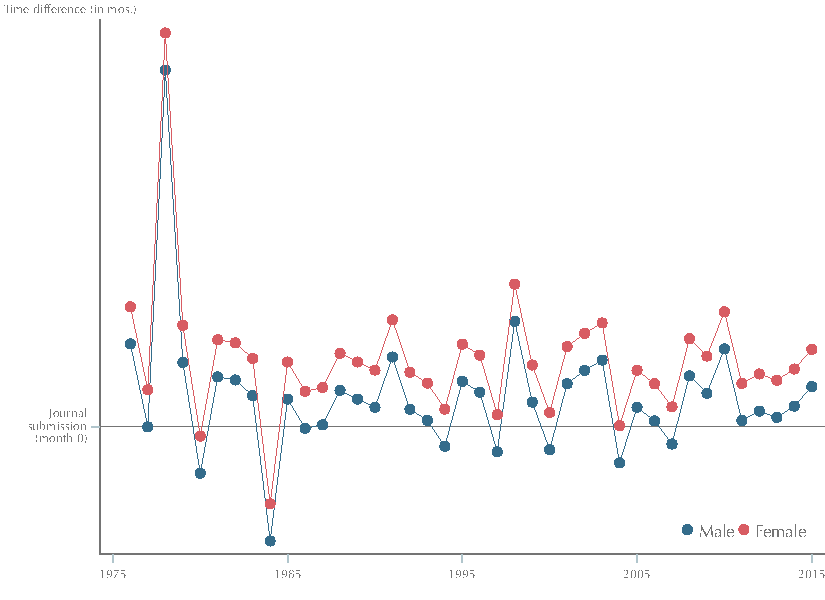
\includegraphics[width=12.3cm]{$HOME/Dropbox/Readability/draft/pdf/figure8.pdf}
		\floatfoot{\tiny \textit{Notes}. Gender differences in the time between the release of a paper as an NBER Working Paper and submission to \textit{Econometrica}. Horizontal grey line denotes that the paper was submitted to \textit{Econometrica} and released as an NBER Working Paper at the same time. Values below this line indicate that papers in a year were, on average, released as an NBER Working Paper before they were submitted to \textit{Econometrica}; values above this line indicate that papers in a year were, on average, submitted first to \textit{Econometrica} and then released as an NBER Working Paper. Points in blue are effect estimated for 100 percent male-authored papers; points in pink are effects estimated for 100 percent female-authored papers.}
	}
\end{figure}

As can be seen in \autoref{figure8}, men and women both generally release their papers as NBER working papers only \emph{after} they've already submitted the paper to \emph{Econometrica}. For women, however, this delay is more pronounced.

\clearpage

\section{\autoref{duration}, supplemental output []}
\label{durationsupplementaloutput}

\subsection{\autoref{table11}, submission year fixed effects}
\label{appendixsubmissionyear}

\autoref{table11XXA} repeats the regressions pre\-sented in \autoref{table11} but using submission year fixed effects in lieu of publication year fixed effects. As discussed in \autoref{Footnote88}, this change narrows the gap in publication times between male- and female-authored papers by about two months.

\input{/USERS/ERINHENGEL/Dropbox/Readability/draft/tex/generated/table11XXa}

\clearpage

\subsection{\autoref{table11}, alternative thresholds for $\text{mother}_j$}
\label{appendixmotherhood}

\autoref{tableC18} repeats the regression pre\-sented in \autoref{table11} column (5), using alternative age thresholds to define motherhood: $\text{mother}_j$ equals 1 if paper $j$'s co-authors are all mothers to children younger than three (first column), four (second column), \emph{etc.} Changing this threshold has little effect on female ratio's coefficient. The coefficients on $\text{mother}_j$ and $\text{birth}_j$ are persistently negative and positive (respectively), although magnitudes and standard errors vary. Remaining coefficients are unaffected.

\begin{table}[H]
    \footnotesize
    \centering
    \begin{threeparttable}
        \caption{\autoref{table11}, alternative thresholds for \(\text{mother}_j\)}
        \label{tableC18}
        \sisetup{round-precision=3}
        \begin{tabular}{p{4cm}SSSSS}
            \toprule
            &{\(\text{Age}<3\)}&{\(\text{Age}<4\)}&{\(\text{Age}<5\)}&{\(\text{Age}<10\)}&{\(\text{Age}<18\)}\\
            \midrule
            Female ratio                  &       5.826***&       6.345***&       6.657***&       6.566***&       6.339***\\
                                          &     (2.168)   &     (2.097)   &     (2.150)   &     (2.176)   &     (2.226)   \\
            Mother                        &      -3.844   &     -10.795** &     -10.677***&      -8.428** &      -4.828   \\
                                          &     (2.393)   &     (4.079)   &     (3.381)   &     (3.594)   &     (3.451)   \\
            Birth                         &       1.325   &       7.726   &       7.321*  &       5.166   &       1.798   \\
                                          &     (3.784)   &     (4.796)   &     (4.268)   &     (4.497)   &     (4.222)   \\
            Max. \(t_j\)                  &      -0.163** &      -0.165** &      -0.163** &      -0.163** &      -0.162** \\
                                          &     (0.070)   &     (0.070)   &     (0.070)   &     (0.070)   &     (0.070)   \\
            No. pages                     &       0.179***&       0.178***&       0.178***&       0.178***&       0.179***\\
                                          &     (0.026)   &     (0.026)   &     (0.026)   &     (0.026)   &     (0.026)   \\
            \(N\)                         &       0.999** &       0.983** &       0.974** &       0.972** &       0.978** \\
                                          &     (0.445)   &     (0.442)   &     (0.442)   &     (0.443)   &     (0.444)   \\
            Order                         &       0.221** &       0.219** &       0.219** &       0.218** &       0.219** \\
                                          &     (0.089)   &     (0.089)   &     (0.089)   &     (0.089)   &     (0.089)   \\
            No. citations                 &       0.000   &       0.000   &       0.000   &       0.000   &       0.000   \\
                                          &     (0.000)   &     (0.000)   &     (0.000)   &     (0.000)   &     (0.000)   \\
            Constant                      &      37.752***&      37.854***&      37.880***&      37.855***&      37.777***\\
                                          &     (2.052)   &     (2.053)   &     (2.055)   &     (2.058)   &     (2.048)   \\
            \midrule
            Editor effects                &           {\ding{51}}   &           {\ding{51}}   &           {\ding{51}}   &           {\ding{51}}   &           {\ding{51}}   \\
            Year effects                  &           {\ding{51}}   &           {\ding{51}}   &           {\ding{51}}   &           {\ding{51}}   &           {\ding{51}}   \\
            Institution effects           &           {\ding{51}}   &           {\ding{51}}   &           {\ding{51}}   &           {\ding{51}}   &           {\ding{51}}   \\
            \bottomrule
        \end{tabular}
        \begin{tablenotes}
            \tiny
            \item \textit{Notes}. Sample 2,626 articles. Coefficients from OLS estimation of~\autoref{equation13} at different age thresholds for \(\text{mother}_j\). In column one, \(\text{mother}_j\) equals one for papers authored exclusively by women with children younger than three; in column two, the age threshold is four; \textit{etc.} Column three corresponds to results presented in~\autoref{table11}. Standard errors clustered by year in parentheses. ***, ** and * statistically significant at 1\%, 5\% and 10\%, respectively.
        \end{tablenotes}
    \end{threeparttable}
\end{table}

\clearpage

\section{\autoref{seumatching}, supplemental anlysis []}
\label{seumatchingsupplementalanlysis}

\subsection{\autoref{seumatching}, co-variate balance}
\label{appendixmatchingbalance}

\autoref{tableC8} compares co-variate balance pre- and post-match. The first column displays averages for the 121 female authors with at least three publications in the data. The first column of the first panel (``Pre-match means'') displays corresponding averages for the 1,553 male authors with three or more publications. The first column of the second panel (``Post-match means'') displays (weighted) averages for the 104 male authors matched with a female author. \autoref{tableC9}, \autoref{tableC10} and \autoref{tableC11} compare co-variate balance when restricted to matched pairs with $\underline D_{ik}\ne0$.

Gender differences are smaller post-match; $t$-statistics are likewise closer to zero. Moreover, co-variates remain well balanced between $\underline D_{ik}>0$ (discrimination against women) and $\underline D_{ik}<0$ (discrimination against men) samples; both resemble averages in the matched sample.

\clearpage

\begin{table}[H]
    \begin{adjustwidth}{-0.085cm}{}
    \footnotesize
    \centering
    \begin{threeparttable}
        \caption{Pre- and post-matching summary statistics}
        \label{tableC8}
        \begin{tabular}{p{3.55cm}S[group-separator={}]@{}S[group-separator={}]@{}S@{}S@{}S[group-separator={}]@{}S@{}S@{}}
            \toprule
            &&\multicolumn{3}{c}{{Pre-match means}}&\multicolumn{3}{c}{{Post-match means}}\\\cmidrule(lr){3-5}\cmidrule(lr){6-8}&{{Women}}&{{Men}}&{{Difference}}&{{\(t\)}}&{{Men}}&{{Difference}}&{\(t\)}\\
            \midrule
            \quad \(T\)         &        4.55&        5.90&       -1.35&       -3.47&        4.33&        0.22&        0.73\\
            \quad Avg. \(N_{it}\)&        2.20&        2.09&        0.11&        1.99&        2.32&       -0.12&       -1.43\\
            \quad Min. order in issue&        2.69&        2.43&        0.26&        1.50&        2.62&        0.07&        0.28\\
            \quad \% first authored by \(i\)&        1.83&        3.34&       -1.51&       -1.58&        3.14&       -1.31&       -1.24\\
            \quad Max. citations&      267.07&      406.62&     -139.56&       -1.78&      279.08&      -12.01&       -0.25\\
            \quad Max. inst. rank&       49.26&       44.42&        4.83&        2.72&       48.12&        1.13&        0.52\\
            \quad Avg. year     &     2003.48&     1995.45&        8.03&        6.89&     2002.28&        1.21&        1.01\\
            \midrule
            \multicolumn{8}{l}{\textbf{Fraction of articles per decade}}\\
            \quad 1950--59      &       -0.00&        0.01&       -0.01&       -1.57&        0.00&       -0.00&       -1.07\\
            \quad 1960--69      &        0.00&        0.04&       -0.04&       -2.87&        0.01&       -0.01&       -1.15\\
            \quad 1970--79      &        0.01&        0.11&       -0.09&       -4.72&        0.03&       -0.01&       -1.12\\
            \quad 1980--89      &        0.08&        0.18&       -0.10&       -4.36&        0.10&       -0.02&       -0.81\\
            \quad 1990--99      &        0.19&        0.21&       -0.02&       -0.99&        0.16&        0.03&        0.90\\
            \quad 2000--09      &        0.41&        0.26&        0.15&        5.90&        0.40&        0.02&        0.41\\
            \quad 2010--15      &        0.31&        0.20&        0.11&        4.19&        0.31&        0.00&        0.03\\
            \midrule
            \multicolumn{8}{l}{\textbf{Fraction of articles per journal}}\\
            \quad \textit{AER}  &        0.39&        0.25&        0.14&        5.52&        0.36&        0.03&        0.76\\
            \quad \textit{Econometrica}&        0.17&        0.34&       -0.17&       -5.12&        0.21&       -0.04&       -1.17\\
            \quad \textit{JPE}  &        0.18&        0.24&       -0.07&       -2.62&        0.22&       -0.04&       -1.17\\
            \quad \textit{QJE}  &        0.27&        0.17&        0.10&        4.78&        0.21&        0.05&        1.60\\
            \midrule
            \quad A General     &        0.04&        0.02&        0.02&        1.58&        0.01&        0.03&        1.50\\
            \quad B Methodology &       -0.00&        0.02&       -0.02&       -1.44&        0.00&        0.00&           \\
            \quad C Quant. methods&        0.64&        0.81&       -0.17&       -1.03&        0.54&        0.11&        0.66\\
            \quad D Microeconomics&        1.64&        1.79&       -0.15&       -0.69&        1.42&        0.21&        0.97\\
            \quad E Macroeconomics&        0.58&        0.62&       -0.05&       -0.37&        0.44&        0.14&        0.97\\
            \quad F International&        0.39&        0.31&        0.08&        0.81&        0.41&       -0.02&       -0.13\\
            \quad G Finance     &        0.60&        0.52&        0.07&        0.68&        0.56&        0.04&        0.24\\
            \quad H Public      &        0.45&        0.36&        0.10&        1.09&        0.39&        0.07&        0.66\\
            \quad I Health, welfare, edu&        0.88&        0.34&        0.53&        5.35&        0.77&        0.10&        0.49\\
            \quad J Labour      &        1.26&        0.76&        0.49&        3.39&        1.09&        0.16&        0.75\\
            \quad K Law and econ&        0.20&        0.14&        0.06&        1.14&        0.21&       -0.01&       -0.12\\
            \quad L Industrial org&        0.73&        0.57&        0.16&        1.46&        0.57&        0.16&        1.15\\
            \quad M Marketing/accounting&        0.17&        0.13&        0.04&        0.92&        0.22&       -0.05&       -0.75\\
            \quad N Economic history&        0.29&        0.14&        0.15&        2.73&        0.14&        0.15&        1.51\\
            \quad O Development &        0.86&        0.52&        0.34&        2.58&        0.88&       -0.02&       -0.08\\
            \quad P Economic systems&        0.08&        0.09&       -0.01&       -0.22&        0.08&       -0.00&       -0.05\\
            \quad Q Agri., environment&        0.18&        0.12&        0.06&        1.20&        0.21&       -0.03&       -0.35\\
            \quad R Regional, transport&        0.17&        0.16&        0.01&        0.16&        0.20&       -0.02&       -0.39\\
            \quad Z Special topics&        0.16&        0.10&        0.06&        1.50&        0.22&       -0.06&       -0.90\\
            \bottomrule
        \end{tabular}
        \begin{tablenotes}
            \tiny
            \item \textit{Notes}. Sample restricted to authors with three or more publications. First panel shows pre-match summary statistics (121 female authors, 1,553 male authors). Second panel shows post-match summary statistics (106 male authors). \(t\)-values for differences reported in columns four and seven.
        \end{tablenotes}
    \end{threeparttable}
    \end{adjustwidth}
\end{table}

\begin{table}[H]
    \begin{adjustwidth}{-0.6cm}{}
    \footnotesize
    \centering
    \begin{threeparttable}
        \caption{Co-variate post-match balance when \(\underline D_{ik}\ne0\)}
        \label{tableC9}
        \sisetup{group-separator={}}
        \begin{tabular}{p{3.55cm}S@{}S@{}S@{}S@{}S@{}S@{}S@{}S@{}}
            \toprule
            &\multicolumn{4}{c}{{Flesch Reading Ease}}&\multicolumn{4}{c}{{Flesch Kincaid}}\\\cmidrule(lr){2-5}\cmidrule(lr){6-9}&\multicolumn{2}{c}{{Discrimination}}&&&\multicolumn{2}{c}{{Discrimination}}&&\\\cmidrule[0.01pt](lr){2-3}\cmidrule[0.01pt](lr){6-7}&{{\crcell[b]{Against\\[-0.1cm]women}}}&{{\crcell[b]{Against\\[-0.1cm]men}}}&{{Difference}}&{{\(t\)}}&{{\crcell[b]{Against\\[-0.1cm]women}}}&{{\crcell[b]{Against\\[-0.1cm]men}}}&{{Difference}}&{{\(t\)}}\\
            \midrule
            \quad \(T\)         &        4.49&        4.34&        0.14&        0.35&        4.65&        4.33&        0.32&        0.78\\
            \quad Avg. \(N_{it}\)&        2.36&        2.27&        0.09&        0.89&        2.37&        2.21&        0.15&        1.71\\
            \quad Min. order in issue&        2.84&        2.67&        0.17&        0.50&        2.87&        2.77&        0.10&        0.31\\
            \quad \% first authored by \(i\)&        3.25&        0.97&        2.29&        1.77&        2.52&        2.32&        0.20&        0.16\\
            \quad Max. citations&      205.77&      260.56&      -54.79&       -1.19&      272.13&      281.17&       -9.04&       -0.17\\
            \quad Max. inst. rank&       50.14&       48.59&        1.56&        0.58&       49.04&       48.79&        0.24&        0.09\\
            \quad Avg. year     &     2003.40&     2004.59&       -1.20&       -0.79&     2003.38&     2004.23&       -0.86&       -0.66\\
            \midrule
            \multicolumn{9}{l}{\textbf{Fraction of articles per decade}}\\
            \quad 1950--59      &        0.01&        0.00&        0.01&        1.00&        0.00&        0.00&        0.00&        1.00\\
            \quad 1960--69      &        0.02&        0.01&        0.01&        1.02&        0.00&        0.00&       -0.00&       -0.00\\
            \quad 1970--79      &        0.02&        0.02&       -0.00&       -0.27&        0.01&        0.02&       -0.00&       -0.07\\
            \quad 1980--89      &        0.06&        0.05&        0.02&        0.65&        0.08&        0.06&        0.02&        0.72\\
            \quad 1990--99      &        0.14&        0.15&       -0.02&       -0.41&        0.15&        0.16&       -0.01&       -0.17\\
            \quad 2000--09      &        0.43&        0.39&        0.03&        0.69&        0.42&        0.42&        0.00&        0.02\\
            \quad 2010--15      &        0.33&        0.38&       -0.05&       -0.93&        0.32&        0.34&       -0.02&       -0.40\\
            \midrule
            \multicolumn{9}{l}{\textbf{Fraction of articles per journal}}\\
            \quad \textit{AER}  &        0.40&        0.39&        0.00&        0.03&        0.39&        0.42&       -0.03&       -0.71\\
            \quad \textit{Econometrica}&        0.18&        0.14&        0.04&        0.83&        0.19&        0.15&        0.04&        0.87\\
            \quad \textit{JPE}  &        0.20&        0.17&        0.03&        0.68&        0.19&        0.16&        0.03&        0.85\\
            \quad \textit{QJE}  &        0.23&        0.29&       -0.07&       -1.58&        0.23&        0.26&       -0.04&       -0.91\\
            \midrule
            \quad A General     &        0.01&        0.03&       -0.01&       -0.58&        0.01&        0.01&        0.00&        0.00\\
            \quad B Methodology &        0.00&        0.00&        0.00&           &        0.00&        0.00&        0.00&           \\
            \quad C Quant. methods&        0.44&        0.39&        0.06&        0.36&        0.37&        0.46&       -0.10&       -0.81\\
            \quad D Microeconomics&        1.51&        1.64&       -0.13&       -0.45&        1.40&        1.71&       -0.30&       -1.20\\
            \quad E Macroeconomics&        0.39&        0.49&       -0.10&       -0.67&        0.48&        0.51&       -0.04&       -0.24\\
            \quad F International&        0.41&        0.34&        0.07&        0.39&        0.50&        0.28&        0.22&        1.35\\
            \quad G Finance     &        0.79&        0.50&        0.29&        1.27&        0.62&        0.67&       -0.05&       -0.24\\
            \quad H Public      &        0.46&        0.49&       -0.03&       -0.21&        0.45&        0.46&       -0.01&       -0.10\\
            \quad I Health, welfare, edu&        1.04&        0.81&        0.23&        0.78&        1.02&        0.90&        0.12&        0.41\\
            \quad J Labour      &        1.33&        1.37&       -0.04&       -0.15&        1.39&        1.32&        0.07&        0.27\\
            \quad K Law and econ&        0.23&        0.21&        0.01&        0.14&        0.23&        0.24&       -0.01&       -0.12\\
            \quad L Industrial org&        0.73&        0.83&       -0.10&       -0.49&        0.74&        0.79&       -0.05&       -0.27\\
            \quad M Marketing/accounting&        0.20&        0.24&       -0.04&       -0.44&        0.24&        0.16&        0.09&        1.07\\
            \quad N Economic history&        0.19&        0.34&       -0.16&       -1.16&        0.12&        0.34&       -0.22&       -1.89\\
            \quad O Development &        0.96&        0.57&        0.39&        1.55&        1.12&        0.73&        0.39&        1.44\\
            \quad P Economic systems&        0.10&        0.13&       -0.03&       -0.37&        0.11&        0.10&        0.01&        0.17\\
            \quad Q Agri., environment&        0.26&        0.14&        0.11&        1.20&        0.29&        0.09&        0.21&        2.40\\
            \quad R Regional, transport&        0.14&        0.19&       -0.04&       -0.53&        0.21&        0.20&        0.01&        0.15\\
            \quad Z Special topics&        0.13&        0.29&       -0.16&       -1.82&        0.22&        0.20&        0.02&        0.30\\
            \bottomrule
        \end{tabular}
        \begin{tablenotes}
            \tiny
            \item \textit{Notes}. Sample restricted to authors with three or more publications. First panel shows pre-match summary statistics. \(t\)-values for differences reported in columns four and seven.
        \end{tablenotes}
    \end{threeparttable}
    \end{adjustwidth}
\end{table}

\begin{table}[H]
    \begin{adjustwidth}{-0.6cm}{}
    \footnotesize
    \centering
    \begin{threeparttable}
        \caption{Co-variate post-match balance when \(\underline D_{ik}\ne0\)}
        \label{tableC10}
        \sisetup{group-separator={}}
        \begin{tabular}{p{3.55cm}S@{}S@{}S@{}S@{}S@{}S@{}S@{}S@{}}
            \toprule
            &\multicolumn{4}{c}{{Gunning Fog}}&\multicolumn{4}{c}{{SMOG}}\\\cmidrule(lr){2-5}\cmidrule(lr){6-9}&\multicolumn{2}{c}{{Discrimination}}&&&\multicolumn{2}{c}{{Discrimination}}&&\\\cmidrule[0.01pt](lr){2-3}\cmidrule[0.01pt](lr){6-7}&{{\crcell[b]{Against\\[-0.1cm]women}}}&{{\crcell[b]{Against\\[-0.1cm]men}}}&{{Difference}}&{{\(t\)}}&{{\crcell[b]{Against\\[-0.1cm]women}}}&{{\crcell[b]{Against\\[-0.1cm]men}}}&{{Difference}}&{{\(t\)}}\\
            \midrule
            \quad \(T\)         &        4.57&        4.09&        0.47&        1.18&        4.72&        4.12&        0.61&        1.45\\
            \quad Avg. \(N_{it}\)&        2.37&        2.23&        0.14&        1.39&        2.34&        2.27&        0.07&        0.73\\
            \quad Min. order in issue&        2.88&        2.67&        0.21&        0.65&        2.76&        2.62&        0.14&        0.46\\
            \quad \% first authored by \(i\)&        2.03&        2.73&       -0.70&       -0.55&        2.57&        3.17&       -0.60&       -0.43\\
            \quad Max. citations&      273.88&      258.13&       15.75&        0.29&      269.43&      261.79&        7.64&        0.14\\
            \quad Max. inst. rank&       48.92&       48.96&       -0.04&       -0.01&       49.87&       47.54&        2.33&        0.87\\
            \quad Avg. year     &     2003.39&     2004.11&       -0.72&       -0.50&     2003.80&     2003.98&       -0.19&       -0.13\\
            \midrule
            \multicolumn{9}{l}{\textbf{Fraction of articles per decade}}\\
            \quad 1950--59      &        0.01&       -0.00&        0.01&        1.00&        0.01&       -0.00&        0.01&        1.00\\
            \quad 1960--69      &        0.01&        0.01&        0.00&        0.00&        0.01&        0.01&        0.00&        0.00\\
            \quad 1970--79      &        0.02&        0.02&        0.00&        0.05&        0.02&        0.03&       -0.01&       -0.70\\
            \quad 1980--89      &        0.08&        0.04&        0.04&        1.33&        0.06&        0.06&        0.00&        0.13\\
            \quad 1990--99      &        0.13&        0.17&       -0.04&       -0.99&        0.14&        0.14&        0.00&        0.03\\
            \quad 2000--09      &        0.42&        0.43&       -0.01&       -0.22&        0.43&        0.43&        0.00&        0.03\\
            \quad 2010--15      &        0.33&        0.33&        0.01&        0.11&        0.33&        0.33&        0.00&        0.02\\
            \midrule
            \multicolumn{9}{l}{\textbf{Fraction of articles per journal}}\\
            \quad \textit{AER}  &        0.40&        0.39&        0.00&        0.09&        0.39&        0.38&        0.01&        0.25\\
            \quad \textit{Econometrica}&        0.19&        0.16&        0.04&        0.79&        0.21&        0.15&        0.07&        1.42\\
            \quad \textit{JPE}  &        0.18&        0.17&        0.01&        0.30&        0.19&        0.19&       -0.00&       -0.02\\
            \quad \textit{QJE}  &        0.23&        0.28&       -0.05&       -1.25&        0.21&        0.29&       -0.08&       -1.82\\
            \midrule
            \quad A General     &        0.01&        0.03&       -0.01&       -0.58&        0.01&        0.03&       -0.01&       -0.58\\
            \quad B Methodology &        0.00&        0.00&        0.00&           &        0.00&        0.00&        0.00&           \\
            \quad C Quant. methods&        0.45&        0.59&       -0.14&       -0.79&        0.61&        0.50&        0.11&        0.55\\
            \quad D Microeconomics&        1.34&        1.55&       -0.21&       -0.86&        1.45&        1.46&       -0.01&       -0.05\\
            \quad E Macroeconomics&        0.42&        0.47&       -0.05&       -0.37&        0.46&        0.43&        0.03&        0.18\\
            \quad F International&        0.51&        0.24&        0.28&        1.77&        0.55&        0.30&        0.25&        1.42\\
            \quad G Finance     &        0.66&        0.45&        0.21&        1.19&        0.78&        0.43&        0.34&        1.67\\
            \quad H Public      &        0.43&        0.46&       -0.03&       -0.21&        0.41&        0.45&       -0.04&       -0.32\\
            \quad I Health, welfare, edu&        1.09&        0.78&        0.32&        1.04&        1.16&        0.82&        0.34&        1.09\\
            \quad J Labour      &        1.30&        1.36&       -0.05&       -0.19&        1.24&        1.34&       -0.11&       -0.38\\
            \quad K Law and econ&        0.24&        0.18&        0.05&        0.56&        0.22&        0.16&        0.07&        0.72\\
            \quad L Industrial org&        0.71&        0.57&        0.14&        0.90&        0.75&        0.67&        0.08&        0.45\\
            \quad M Marketing/accounting&        0.18&        0.14&        0.04&        0.56&        0.16&        0.16&        0.00&        0.00\\
            \quad N Economic history&        0.13&        0.37&       -0.24&       -1.90&        0.14&        0.33&       -0.18&       -1.53\\
            \quad O Development &        1.17&        0.74&        0.43&        1.52&        1.13&        0.67&        0.46&        1.63\\
            \quad P Economic systems&        0.13&        0.12&        0.01&        0.16&        0.13&        0.12&        0.01&        0.16\\
            \quad Q Agri., environment&        0.28&        0.12&        0.16&        1.70&        0.28&        0.16&        0.12&        1.22\\
            \quad R Regional, transport&        0.21&        0.18&        0.03&        0.31&        0.18&        0.20&       -0.01&       -0.16\\
            \quad Z Special topics&        0.22&        0.22&        0.00&        0.00&        0.18&        0.22&       -0.04&       -0.48\\
            \bottomrule
        \end{tabular}
        \begin{tablenotes}
            \tiny
            \item \textit{Notes}. Sample restricted to authors with three or more publications. First panel shows pre-match summary statistics. \(t\)-values for differences reported in columns four and seven.
        \end{tablenotes}
    \end{threeparttable}
    \end{adjustwidth}
\end{table}

\begin{table}[H]
    \footnotesize
    \centering
    \begin{threeparttable}
        \caption{Co-variate post-match balance when \(\underline D_{ik}\ne0\)}
        \label{tableC11}
        \sisetup{group-separator={}}
        \begin{tabular}{p{3.55cm}S@{}S@{}S@{}S@{}}
            \toprule
            &\multicolumn{4}{c}{{Dale-Chall}}\\\cmidrule(lr){2-5}&\multicolumn{2}{c}{{Discrimination}}&&\\\cmidrule[0.01pt](lr){2-3}&{{\crcell[b]{Against\\[-0.1cm]women}}}&{{\crcell[b]{Against\\[-0.1cm]men}}}&{{Difference}}&{{\(t\)}}\\
            \midrule
            \quad \(T\)         &        4.91&        4.64&        0.27&        0.55\\
            \quad Avg. \(N_{it}\)&        2.23&        2.27&       -0.04&       -0.39\\
            \quad Min. order in issue&        2.84&        2.59&        0.26&        0.77\\
            \quad \% first authored by \(i\)&        2.66&        2.25&        0.41&        0.29\\
            \quad Max. citations&      250.76&      318.26&      -67.50&       -0.98\\
            \quad Max. inst. rank&       47.40&       49.37&       -1.97&       -0.68\\
            \quad Avg. year     &     2003.85&     2002.82&        1.04&        0.69\\
            \midrule
            \multicolumn{5}{l}{\textbf{Fraction of articles per decade}}\\
            \quad 1950--59      &       -0.00&        0.01&       -0.01&       -1.00\\
            \quad 1960--69      &        0.01&        0.01&       -0.01&       -0.67\\
            \quad 1970--79      &        0.02&        0.01&        0.01&        0.68\\
            \quad 1980--89      &        0.06&        0.10&       -0.04&       -1.17\\
            \quad 1990--99      &        0.15&        0.17&       -0.02&       -0.42\\
            \quad 2000--09      &        0.45&        0.39&        0.05&        1.03\\
            \quad 2010--15      &        0.32&        0.31&        0.01&        0.11\\
            \midrule
            \multicolumn{5}{l}{\textbf{Fraction of articles per journal}}\\
            \quad \textit{AER}  &        0.44&        0.35&        0.09&        1.98\\
            \quad \textit{Econometrica}&        0.16&        0.18&       -0.01&       -0.26\\
            \quad \textit{JPE}  &        0.15&        0.20&       -0.05&       -1.28\\
            \quad \textit{QJE}  &        0.25&        0.27&       -0.03&       -0.65\\
            \midrule
            \quad A General     &        0.03&        0.01&        0.01&        0.58\\
            \quad B Methodology &        0.00&        0.00&        0.00&           \\
            \quad C Quant. methods&        0.37&        0.49&       -0.11&       -0.84\\
            \quad D Microeconomics&        1.80&        1.59&        0.21&        0.72\\
            \quad E Macroeconomics&        0.57&        0.29&        0.29&        1.95\\
            \quad F International&        0.43&        0.34&        0.09&        0.49\\
            \quad G Finance     &        0.79&        0.41&        0.37&        1.65\\
            \quad H Public      &        0.53&        0.41&        0.11&        0.84\\
            \quad I Health, welfare, edu&        1.23&        0.99&        0.24&        0.70\\
            \quad J Labour      &        1.49&        1.51&       -0.03&       -0.09\\
            \quad K Law and econ&        0.24&        0.27&       -0.03&       -0.27\\
            \quad L Industrial org&        0.71&        0.79&       -0.07&       -0.37\\
            \quad M Marketing/accounting&        0.17&        0.26&       -0.09&       -1.00\\
            \quad N Economic history&        0.31&        0.23&        0.09&        0.62\\
            \quad O Development &        1.13&        0.89&        0.24&        0.74\\
            \quad P Economic systems&        0.19&        0.11&        0.07&        0.81\\
            \quad Q Agri., environment&        0.29&        0.20&        0.09&        0.75\\
            \quad R Regional, transport&        0.17&        0.11&        0.06&        0.74\\
            \quad Z Special topics&        0.21&        0.29&       -0.07&       -0.69\\
            \bottomrule
        \end{tabular}
        \begin{tablenotes}
            \tiny
            \item \textit{Notes}. Sample restricted to authors with three or more publications. First panel shows pre-match summary statistics. \(t\)-values for differences reported in columns four and seven.
        \end{tablenotes}
    \end{threeparttable}
\end{table}

\clearpage

\subsection{\autoref{seumatching}, $\widehat R_{it}$ regression output}
\label{appendixreconstruction}

\autoref{tableC12} and \autoref{tableC13} displays output from time- and gender-specific regressions used to generate $\widehat R_{it}$. (Output for male authors at $t=1$ not shown.)

\begin{table}[H]
    \footnotesize
    \centering
    \begin{threeparttable}
        \caption{Regression output generating \(\widehat R_{it}\)}
        \label{tableC12}
        \sisetup{group-separator={}}
        \begin{tabular}{p{2.5cm}SSSSSS}
            \toprule
            &\multicolumn{3}{c}{{Flesch Reading Ease}}&\multicolumn{3}{c}{{Flesch-Kincaid}}\\\cmidrule[0.01pt](lr){2-4}\cmidrule[0.01pt](lr){5-7}&\multicolumn{2}{c}{{Women}}&{{Men}}&\multicolumn{2}{c}{{Women}}&{{Men}}\\\cmidrule(lr){2-3}\cmidrule(lr){4-4}\cmidrule(lr){5-6}\cmidrule(lr){7-7}&{{\(t=1\)}}&{{\(t=3\)}}&{{\(t=3\)}}&{{\(t=1\)}}&{{\(t=3\)}}&{{\(t=3\)}}\\
            \midrule
            Female ratio                  &        4.36   &        3.89   &        9.29   &       -0.09   &        0.74   &        2.91*  \\
                                          &      (7.68)   &      (5.96)   &      (6.41)   &      (1.59)   &      (1.21)   &      (1.70)   \\
            \(N\)                         &        1.33   &        0.14   &        0.47   &       -0.01   &       -0.07   &        0.25   \\
                                          &      (2.47)   &      (1.89)   &      (1.03)   &      (0.51)   &      (0.38)   &      (0.27)   \\
            Inst. rank                    &       -0.03   &       -0.15*  &        0.09   &        0.00   &       -0.03   &        0.01   \\
                                          &      (0.11)   &      (0.08)   &      (0.07)   &      (0.02)   &      (0.02)   &      (0.02)   \\
            Max. inst. rank               &        0.07   &        0.18   &       -0.12   &        0.01   &        0.03   &       -0.02   \\
                                          &      (0.13)   &      (0.11)   &      (0.09)   &      (0.03)   &      (0.02)   &      (0.02)   \\
            Max. \(t_j\)                  &       -0.57*  &       -0.23   &        0.33** &       -0.06   &       -0.00   &        0.10** \\
                                          &      (0.34)   &      (0.29)   &      (0.14)   &      (0.07)   &      (0.06)   &      (0.04)   \\
            Year                          &        0.21   &        0.03   &       -0.11   &        0.04   &        0.03   &       -0.07** \\
                                          &      (0.13)   &      (0.13)   &      (0.12)   &      (0.03)   &      (0.03)   &      (0.03)   \\
            \textit{Econometrica}         &       -3.03   &       -4.25   &       -1.04   &       -1.37*  &       -0.80   &       -0.14   \\
                                          &      (3.90)   &      (3.10)   &      (3.17)   &      (0.81)   &      (0.63)   &      (0.84)   \\
            \textit{JPE}                  &        1.05   &        1.63   &        9.44***&        0.19   &        0.16   &        1.60*  \\
                                          &      (3.39)   &      (3.34)   &      (3.26)   &      (0.70)   &      (0.68)   &      (0.87)   \\
            \textit{QJE}                  &        4.95   &        0.38   &        0.48   &        0.38   &       -0.31   &        0.67   \\
                                          &      (3.05)   &      (2.66)   &      (2.52)   &      (0.63)   &      (0.54)   &      (0.67)   \\
            Constant                      &     -389.75   &      -23.30   &      256.50   &      -97.19*  &      -75.18   &      129.07*  \\
                                          &    (265.17)   &    (262.33)   &    (249.21)   &     (55.07)   &     (53.33)   &     (66.27)   \\
            \bottomrule
        \end{tabular}
        \begin{tablenotes}
            \tiny
            \item \textit{Notes}. Sample 121 female authors; 106 male authors. Sample restricted to matched authors. See~\autoref{seumatching} for details on how matches were made. Regressions weighted by the frequency observations are used in a match. Standard errors in parentheses. ***, ** and * statistically significant at 1\%, 5\% and 10\%, respectively.
        \end{tablenotes}
    \end{threeparttable}
\end{table}

\begin{landscape}
\begin{table}
    \footnotesize
    \centering
    \begin{threeparttable}
        \caption{Regression output generating \(\widehat R_{it}\)}
        \label{tableC13}
        \sisetup{group-separator={}}
        \begin{tabular}{p{2.5cm}SSSSSSSSS}
            \toprule
            &\multicolumn{3}{c}{{Gunning Fog}}&\multicolumn{3}{c}{{SMOG}}&\multicolumn{3}{c}{{Dale-Chall}}\\\cmidrule[0.01pt](lr){2-4}\cmidrule[0.01pt](lr){5-7}\cmidrule[0.01pt](lr){8-10}&\multicolumn{2}{c}{{Women}}&{{Men}}&\multicolumn{2}{c}{{Women}}&{{Men}}&\multicolumn{2}{c}{{Women}}&{{Men}}\\\cmidrule(lr){2-3}\cmidrule(lr){4-4}\cmidrule(lr){5-6}\cmidrule(lr){7-7}\cmidrule(lr){8-9}\cmidrule(lr){10-10}&{{\(t=1\)}}&{{\(t=3\)}}&{{\(t=3\)}}&{{\(t=1\)}}&{{\(t=3\)}}&{{\(t=3\)}}&{{\(t=1\)}}&{{\(t=3\)}}&{{\(t=3\)}}\\
            \midrule
            Female ratio                  &       -0.85   &        1.14   &        3.39*  &       -0.36   &        0.90   &        1.87   &        0.28   &        0.31   &        2.15***\\
                                          &      (1.93)   &      (1.50)   &      (1.79)   &      (1.40)   &      (1.11)   &      (1.18)   &      (0.61)   &      (0.58)   &      (0.53)   \\
            \(N\)                         &       -0.10   &       -0.05   &        0.37   &       -0.01   &        0.01   &        0.20   &        0.08   &       -0.05   &        0.03   \\
                                          &      (0.62)   &      (0.47)   &      (0.29)   &      (0.45)   &      (0.35)   &      (0.19)   &      (0.19)   &      (0.18)   &      (0.09)   \\
            Inst. rank                    &        0.01   &       -0.02   &        0.03   &        0.00   &       -0.02   &        0.02*  &       -0.01   &       -0.02** &        0.01   \\
                                          &      (0.03)   &      (0.02)   &      (0.02)   &      (0.02)   &      (0.02)   &      (0.01)   &      (0.01)   &      (0.01)   &      (0.01)   \\
            Max. inst. rank               &        0.01   &        0.02   &       -0.03   &        0.01   &        0.02   &       -0.03   &        0.01   &        0.02   &       -0.02** \\
                                          &      (0.03)   &      (0.03)   &      (0.03)   &      (0.02)   &      (0.02)   &      (0.02)   &      (0.01)   &      (0.01)   &      (0.01)   \\
            Max. \(t_j\)                  &       -0.11   &       -0.00   &        0.11***&       -0.10   &       -0.01   &        0.07** &       -0.04   &       -0.02   &        0.00   \\
                                          &      (0.08)   &      (0.07)   &      (0.04)   &      (0.06)   &      (0.05)   &      (0.03)   &      (0.03)   &      (0.03)   &      (0.01)   \\
            Year                          &        0.04   &        0.02   &       -0.05   &        0.04   &        0.01   &       -0.01   &        0.02** &       -0.01   &       -0.01   \\
                                          &      (0.03)   &      (0.03)   &      (0.03)   &      (0.02)   &      (0.02)   &      (0.02)   &      (0.01)   &      (0.01)   &      (0.01)   \\
            \textit{Econometrica}         &       -1.65*  &       -1.32*  &       -0.19   &       -0.78   &       -0.96*  &       -0.27   &       -0.61*  &       -0.45   &       -0.46*  \\
                                          &      (0.98)   &      (0.78)   &      (0.89)   &      (0.71)   &      (0.58)   &      (0.58)   &      (0.31)   &      (0.30)   &      (0.26)   \\
            \textit{JPE}                  &       -0.11   &        0.29   &        1.85** &       -0.04   &        0.40   &        1.48** &       -0.11   &        0.25   &        0.96***\\
                                          &      (0.85)   &      (0.84)   &      (0.91)   &      (0.62)   &      (0.62)   &      (0.60)   &      (0.27)   &      (0.33)   &      (0.27)   \\
            \textit{QJE}                  &        0.65   &       -0.42   &        0.39   &        0.61   &       -0.23   &       -0.09   &        0.46*  &        0.30   &        0.05   \\
                                          &      (0.77)   &      (0.67)   &      (0.70)   &      (0.56)   &      (0.49)   &      (0.46)   &      (0.24)   &      (0.26)   &      (0.21)   \\
            Constant                      &     -101.85   &      -60.54   &       73.41   &      -90.57*  &      -43.47   &       -3.89   &      -58.39***&       11.32   &        5.48   \\
                                          &     (66.54)   &     (65.93)   &     (69.63)   &     (48.45)   &     (48.80)   &     (45.82)   &     (20.94)   &     (25.56)   &     (20.68)   \\
            \bottomrule
        \end{tabular}
        \begin{tablenotes}
            \tiny
            \item \textit{Notes}. Sample 121 female authors; 106 male authors. Sample restricted to matched authors. See~\autoref{seumatching} for details on how matches were made. Regressions weighted by the frequency observations are used in a match. Standard errors in parentheses. ***, ** and * statistically significant at 1\%, 5\% and 10\%, respectively.
        \end{tablenotes}
    \end{threeparttable}
\end{table}
\end{landscape}


\subsection{\autoref{seumatching}, list of matched pairs}
\label{appendixmatchingnames}

\autoref{tableC14} displays the names of the economists in each matched pair.

\begin{ThreePartTable}
    \begin{TableNotes}
        \tiny\item \textit{Notes}. Table lists the names of the matched pairs from~\autoref{seumatching}. In each panel, female members are listed first; male members second. Matches were made using a probit model with replacement. See~\autoref{seumatching} for details on the matching process.
    \end{TableNotes}
    {\scriptsize\begin{longtable}[c]{llll}
        \caption{List of matched pairs}\label{tableC14} \\
        \toprule
        \multicolumn{2}{c}{Matched pairs}&\multicolumn{2}{c}{Matched pairs}\\\cmidrule(lr){1-2}\cmidrule(lr){3-4}Female&Male&Female&Male \\
        \midrule
        \endfirsthead
        \multicolumn{4}{c}{\normalsize{\tablename~\thetable{} (continued)}} \\
        \toprule
        \multicolumn{2}{c}{Matched pairs}&\multicolumn{2}{c}{Matched pairs}\\\cmidrule(lr){1-2}\cmidrule(lr){3-4}Female&Male&Female&Male \\
        \midrule
        \endhead
        \midrule
        \endfoot
        \bottomrule
        \insertTableNotes
        \endlastfoot
            Abraham, Katharine G.&Stahl, Dale O. (II)&Kuziemko, Ilyana&Benjamin, Daniel J.\\
            Admati, Anat R.&Saloner, Garth&La Ferrara, Eliana&Dessein, Wouter\\
            Amiti, Mary&Moav, Omer&Landes, Elisabeth M.&Williams, John C.\\
            Anderson, Siwan&Nunn, Nathan&Levy, Gilat&Costinot, Arnaud\\
            Ashraf, Nava&Kane, Thomas J.&Lewis, Karen K.&Bronnenberg, Bart J.\\
            Athey, Susan&Roemer, John E.&Li, Wei&Scholz, John Karl\\
            Baicker, Katherine&Pop-Eleches, Cristian&Lleras-Muney, Adriana&Salvanes, Kjell G.\\
            Bailey, Martha J.&Wacziarg, Romain&Løken, Katrine Vellesen&Kane, Thomas J.\\
            Bandiera, Oriana&Handel, Benjamin R.&Madrian, Brigitte C.&Topa, Giorgio\\
            Barwick, Panle Jia&Wolitzky, Alexander&Maestas, Nicole&Knittel, Christopher R.\\
            Baxter, Marianne&Blau, David M.&Malmendier, Ulrike&Autor, David H.\\
            Bedard, Kelly&Oreopoulos, Philip&Matzkin, Rosa L.&Sherman, Roger\\
            Bertrand, Marianne&Martimort, David&McConnell, Sheena&Olken, Benjamin A.\\
            Black, Sandra E.&Gowrisankaran, Gautam&McGrattan, Ellen R.&Spiegler, Ran\\
            Blank, Rebecca M.&Rasul, Imran&Meyer, Margaret A.&Brunnermeier, Markus K.\\
            Boustan, Leah Platt&Hatfield, John William&Molinari, Francesca&Stegeman, Mark\\
            Brown, Jennifer&Schorfheide, Frank&Moser, Petra&Dahl, Gordon B.\\
            Busse, Meghan R.&Kellogg, Ryan&Nakamura, Emi&Duffy, John\\
            Case, Anne C.&Schmidt, Klaus M.&Ng, Serena&Fershtman, Chaim\\
            Casella, Alessandra&Ireland, Peter N.&Niederle, Muriel&Zinman, Jonathan\\
            Chen, Xiaohong&Schultz, Theodore W.&Oster, Emily&Jensen, Robert T.\\
            Chen, Yan&Wolitzky, Alexander&Pande, Rohini&Carrell, Scott E.\\
            Chevalier, Judith A.&Beaudry, Paul&Paxson, Christina H.&Piccione, Michele\\
            Chichilnisky, Graciela&Libecap, Gary D.&Perrigne, Isabelle&Fisher, Anthony C.\\
            Correia, Isabel&Zinman, Jonathan&Piazzesi, Monika&Fisher, Jonas D. M.\\
            Costa, Dora L.&Rose, Andrew K.&Qian, Nancy&Woodruff, Christopher\\
            Cropper, Maureen L.&Vytlacil, Edward J.&Quinzii, Martine&Cox, James C.\\
            Currie, Janet&Kellogg, Ryan&Ramey, Valerie A.&Brown, James N.\\
            Dafny, Leemore S.&Miguel, Edward&Reinganum, Jennifer F.&Lagos, Ricardo\\
            De Nardi, Mariacristina&Knittel, Christopher R.&Reinhart, Carmen M.&Broda, Christian\\
            Demange, Gabrielle&Rogerson, William P.&Rey, Hélène&Manovskii, Iourii\\
            Duflo, Esther&Bettinger, Eric P.&Romer, Christina D.&Samuelson, Paul A.\\
            Dupas, Pascaline&Kremer, Michael&Rose-Ackerman, Susan&Bollerslev, Tim\\
            Dynan, Karen E.&Liebman, Jeffrey B.&Rose, Nancy L.&Sørensen, Peter Norman\\
            Eberly, Janice C.&Gordon, Robert J.&Rosenblat, Tanya S.&Brown, Jeffrey R.\\
            Eckel, Catherine C.&Bernhardt, Dan&Rouse, Cecilia Elena&Svensson, Jakob\\
            Edlund, Lena&Libecap, Gary D.&Sapienza, Paola&Brown, Jeffrey R.\\
            Eyigungor, Burcu&Spolaore, Enrico&Schennach, Susanne M.&Moskowitz, Tobias J.\\
            Fan, Yanqin&Rauch, James E.&Schmitt-Grohé, Stephanie&Compte, Olivier\\
            Fernández, Raquel&Salvanes, Kjell G.&Schwartz, Nancy L.&Charnes, Abraham\\
            Field, Erica&Kremer, Michael&Shannon, Chris&Tsyvinski, Aleh\\
            Finkelstein, Amy&Nevo, Aviv&Shaw, Kathryn L.&Lerner, Josh\\
            Flavin, Marjorie A.&Ríos-Rull, José-Víctor&Spier, Kathryn E.&Waugh, Michael E.\\
            Forges, Françoise&Oates, Wallace E.&Stokey, Nancy L.&Ledyard, John O.\\
            Fortin, Nicole M.&Calvó-Armengol, Antoni&Tenreyro, Silvana&Edlin, Aaron S.\\
            Freund, Caroline&Berman, Eli&Tertilt, Michèle&Segerstrom, Paul S.\\
            Fuchs-Schündeln, Nicola&Schmitz, James A. (Jr.)&Tesar, Linda L.&Ackerberg, Daniel A.\\
            Garfinkel, Michelle R.&Zinman, Jonathan&Thomas, Julia K.&Perron, Pierre\\
            Goldberg, Pinelopi Koujianou&Tornell, Aarón&Todd, Petra E.&Gould, Eric D.\\
            Goldin, Claudia D.&Ventura, Jaume&Vissing-Jørgense, Annette&van Wincoop, Eric\\
            Gopinath, Gita&Rayo, Luis&Voena, Alessandra&Bettinger, Eric P.\\
            Griffith, Rachel&Paserman, M. Daniele&Washington, Ebonya L.&Smith, Jeffrey\\
            Guerrieri, Veronica&Huberman, Gur&White, Lucy&Carroll, Gabriel D.\\
            Hanna, Rema&Yuchtman, Noam&Whited, Toni M.&Quah, Danny\\
            Hastings, Justine S.&Bursztyn, Leonardo&Williams, Heidi L.&Gertler, Paul J.\\
            Ho, Katherine&Gould, Eric D.&Wooders, Myrna Holtz&Einav, Liran\\
            Hoxby, Caroline Minter&Carneiro, Pedro&Yariv, Leeat&Ireland, Peter N.\\
            İmrohoroğlu, Ayşe&Smith, Tim R.&Yellen, Janet L.&Hochman, Oded\\
            Jayachandran, Seema&Dahl, Gordon B.&Zeiler, Kathryn&Ireland, Peter N.\\
            Kowalski, Amanda E.&Cameron, Stephen V.&Zhuravskaya, Ekaterina&Djankov, Simeon\\
            Kranton, Rachel E.&Urquiola, Miguel&&\\
    \end{longtable}}
\end{ThreePartTable}


\clearpage

\subsection{\autoref{table10}, male effects, \autoref{equation12} and Condition 1}
\label{appendixconservative}

\autoref{tableC15} estimates $D_{ik}$ with \autoref{equation12}. \autoref{tableC16} estimates $D_{ik}$ with a rough attempt to control for acceptance rates---it requires $T_i\le T_k$ or $T_k\le T_i$ before categorising matched pairs as discrimination against $i$ or $k$, respectively. Conclusions from both tables are are similar to those presented in \autoref{seumatching}.

\begin{table}[H]
    \footnotesize
    \centering
    \begin{threeparttable}
        \caption{\(D_{ik}\),~\autoref{equation12}}
        \label{tableC15}
        \begin{tabular}{p{3cm}S[table-format=3.3]@{}S[table-format=3.3]@{}S[table-format=3.2]@{}S[table-format=4.3]@{}S[table-format=3.3]@{}S[table-format=3.1]@{}S@{}S@{}}
            \toprule
            &\multicolumn{3}{c}{{\crcell[b]{Discrimination against\\[-0.1cm]women (\(\underline{D}_{ik}>0\))}}}&\multicolumn{3}{c}{{\crcell[b]{Discrimination against\\[-0.1cm]men (\(\underline{D}_{ik}<0\))}}}&\multicolumn{2}{c}{{\crcell[b]{Mean, all\\[-0.1cm]observations}}}\\\cmidrule(lr){2-4}\cmidrule(lr){5-7}\cmidrule(lr){8-9}&{{Mean}}&{{S.D.}}&{{\(N\)}}&{{Mean}}&{{S.D.}}&{{\(N\)}}&{{(1)}}&{{(2)}}\\
            \midrule
            Flesch Reading Ease           &        9.07&        6.25&          57&       -5.38&        4.76&          13&        3.79***&        2.69***\\
                                          &            &            &            &            &            &            &      (0.78)   &      (0.91)   \\
            Flesch Kincaid                &        1.81&        1.40&          70&       -1.28&        0.78&          12&        1.01***&        0.86***\\
                                          &            &            &            &            &            &            &      (0.17)   &      (0.19)   \\
            Gunning Fog                   &        2.47&        1.59&          66&       -1.54&        0.77&          10&        1.32***&        1.10***\\
                                          &            &            &            &            &            &            &      (0.21)   &      (0.24)   \\
            SMOG                          &        1.65&        1.15&          61&       -1.33&        0.84&          15&        0.71***&        0.53***\\
                                          &            &            &            &            &            &            &      (0.15)   &      (0.17)   \\
            Dale-Chall                    &        0.85&        0.68&          43&       -0.52&        0.45&          27&        0.20** &        0.12   \\
                                          &            &            &            &            &            &            &      (0.08)   &      (0.09)   \\
            \bottomrule
        \end{tabular}
        \begin{tablenotes}
            \tiny
            \item \textit{Notes}. Sample 121 matched pairs (106 and 121 distinct men and women, respectively). First and second panels display conditional means, standard deviations and observation counts of \(\underline D_{ik}\) (\autoref{equation12}) from subpopulations of matched pairs in which the woman or man, respectively, satisfies Conditions 1 and 2. Third panel displays mean \(\underline D_{ik}\) over all observations. To account for the 30--40 percent of pairs for which ~\autoref{Theorem1} is inconclusive, (1) sets \(\underline D_{ik}=0\), while (2) sets \(\underline D_{ik}=\widehat R_{i3}-\widehat R_{k3}\) if \(\widehat R_{i3}<\widehat R_{k3}\) (\(i\) female, \(k\) male) and zero, otherwise. Male scores are subtracted from female scores; \(\underline D_{ik}\) is positive in panel one and negative in panel two. \(\underline D_{ik}\) weighted by frequency observations are used in a match; degrees-of-freedom corrected standard errors in parentheses (panel three, only). ***, ** and * statistically significant at 1\%, 5\% and 10\%, respectively.
        \end{tablenotes}
    \end{threeparttable}
\end{table}

\begin{table}[H]
    \footnotesize
    \centering
    \begin{threeparttable}
        \caption{\(D_{ik}\), proxying for acceptance rates (Condition 3)}
        \label{tableC16}
        \begin{tabular}{p{3cm}S[table-format=3.3]@{}S[table-format=3.3]@{}S[table-format=3.2]@{}S[table-format=4.3]@{}S[table-format=3.3]@{}S[table-format=3.1]@{}S@{}S@{}}
            \toprule
            &\multicolumn{3}{c}{{\crcell[b]{Discrimination against\\[-0.1cm]women (\(\underline{D}_{ik}>0\))}}}&\multicolumn{3}{c}{{\crcell[b]{Discrimination against\\[-0.1cm]men (\(\underline{D}_{ik}<0\))}}}&\multicolumn{2}{c}{{\crcell[b]{Mean, all\\[-0.1cm]observations}}}\\\cmidrule(lr){2-4}\cmidrule(lr){5-7}\cmidrule(lr){8-9}&{{Mean}}&{{S.D.}}&{{\(N\)}}&{{Mean}}&{{S.D.}}&{{\(N\)}}&{{(1)}}&{{(2)}}\\
            \midrule
            Flesch Reading Ease           &       15.03&       10.52&          34&      -11.39&        9.91&          12&        3.66** &        2.27   \\
                                          &            &            &            &            &            &            &      (1.45)   &      (1.57)   \\
            Flesch Kincaid                &        3.44&        2.09&          46&       -2.46&        1.68&          11&        1.43***&        1.25***\\
                                          &            &            &            &            &            &            &      (0.35)   &      (0.37)   \\
            Gunning Fog                   &        4.03&        2.37&          45&       -3.37&        2.01&           9&        1.57***&        1.30***\\
                                          &            &            &            &            &            &            &      (0.39)   &      (0.42)   \\
            SMOG                          &        2.88&        1.79&          40&       -2.52&        1.63&          14&        0.80***&        0.58*  \\
                                          &            &            &            &            &            &            &      (0.28)   &      (0.31)   \\
            Dale-Chall                    &        1.43&        0.97&          24&       -0.98&        0.83&          20&        0.16   &        0.06   \\
                                          &            &            &            &            &            &            &      (0.14)   &      (0.15)   \\
            \bottomrule
        \end{tabular}
        \begin{tablenotes}
            \tiny
            \item \textit{Notes}. Sample 121 matched pairs (106 and 121 distinct men and women, respectively). First and second panels display conditional means, standard deviations and observation counts of \(\underline D_{ik}\) (\autoref{equation11}) from subpopulations of matched pairs in which the woman or man, respectively, satisfies Conditions 1--3. Third panel displays mean \(\underline D_{ik}\) over all observations. To account for the 30--40 percent of pairs for which ~\autoref{Theorem1} is inconclusive, (1) sets \(\underline D_{ik}=0\), while (2) sets \(\underline D_{ik}=\widehat R_{i3}-\widehat R_{k3}\) if \(\widehat R_{i3}<\widehat R_{k3}\) (\(i\) female, \(k\) male) and zero, otherwise. Male scores are subtracted from female scores; \(\underline D_{ik}\) is positive in panel one and negative in panel two. \(\underline D_{ik}\) weighted by frequency observations are used in a match; degrees-of-freedom corrected standard errors in parentheses (panel three, only). ***, ** and * statistically significant at 1\%, 5\% and 10\%, respectively.
        \end{tablenotes}
    \end{threeparttable}
\end{table}

--$>$

\subsection{\autoref{seumatching}, Mahalanobis matching}
\label{appendixmahalanobis}

\autoref{table9XA}, \autoref{table10XA} and \autoref{figure4XA} replicate the analysis in \autoref{seumatching} but instead of using propensity score matching to generate matched pairs, it uses a Mahalanobis matching procedure. The names of the economists in each matched pair are displayed in \autoref{tableC14XA}. The variables used to match authors are identical to those used for the matches based on propensity scores, outlined in \autoref{seumatching}.

\begin{table}[H]
    \footnotesize
    \centering
    \begin{threeparttable}
        \caption{\autoref{table9}, Mahalanobis Matching}
        \label{table9XA}
        \sisetup{table-format=5.4,round-precision=3}
        \begin{tabular}{p{3.5cm}S@{}S@{}S@{}S@{}S@{}}
            \toprule
            &{\crcell[b]{Flesch\\[-0.1cm]Reading\\[-0.1cm]Ease}}&{\crcell[b]{Flesch-\\[-0.1cm] Kincaid}}&{\crcell[b]{Gunning\\[-0.1cm]Fog}}&{SMOG}&{\crcell[b]{Dale-\\[-0.1cm]Chall}}\\
            \midrule
            \multicolumn{6}{l}{Condition 1}\\
            \quad \(\widehat R_{i3}-\widehat R_{k3}\)&       2.372   &       0.718** &       0.957** &       0.642** &       0.177   \\
                                          &     (1.572)   &     (0.330)   &     (0.392)   &     (0.286)   &     (0.139)   \\
            \midrule\multicolumn{6}{l}{Condition 2}\\
            \quad \(\widehat R_{i3}-\widehat R_{i1}\) (women)&       4.040***&       0.855***&       1.256***&       0.742***&      -0.036   \\
                                          &     (1.544)   &     (0.316)   &     (0.388)   &     (0.285)   &     (0.133)   \\
            \quad \(\widehat R_{k3}-\widehat R_{k1}\) (men)&      -1.508   &      -0.963***&      -1.033** &      -0.589** &      -0.257*  \\
                                          &     (1.551)   &     (0.331)   &     (0.406)   &     (0.292)   &     (0.134)   \\
            \bottomrule
        \end{tabular}
        \begin{tablenotes}
            \tiny
            \item \textit{Notes}. Sample matched pairs (and distinct men and women, respectively). Table displays estimates identical to those in~\autoref{table9}, except that a Mahalanobis distance is used to generate matched pairs. ***, ** and * statistically significant at 1\%, 5\% and 10\%, respectively.
        \end{tablenotes}
    \end{threeparttable}
\end{table}

\begin{table}[H]
    \footnotesize
    \centering
    \begin{threeparttable}
        \caption{\autoref{table10}, Mahalanobis matching}
        \label{table10XA}
        \begin{tabular}{p{3cm}S[table-format=3.3]@{}S[table-format=3.3]@{}S[table-format=3.2]@{}S[table-format=4.3]@{}S[table-format=3.3]@{}S[table-format=3.1]@{}S@{}S@{}}
            \toprule
            &\multicolumn{3}{c}{{\crcell[b]{Discrimination against\\[-0.1cm]women (\(\underline{D}_{ik}>0\))}}}&\multicolumn{3}{c}{{\crcell[b]{Discrimination against\\[-0.1cm]men (\(\underline{D}_{ik}<0\))}}}&\multicolumn{2}{c}{{\crcell[b]{Mean, all\\[-0.1cm]observations}}}\\\cmidrule(lr){2-4}\cmidrule(lr){5-7}\cmidrule(lr){8-9}&{{Mean}}&{{S.D.}}&{{\(N\)}}&{{Mean}}&{{S.D.}}&{{\(N\)}}&{{(1)}}&{{(2)}}\\
            \midrule
            Flesch Reading Ease           &       12.34&       10.05&          48&      -11.13&        9.50&          34&        2.40*  &        1.06   \\
                                          &            &            &            &            &            &            &      (1.40)   &      (1.48)   \\
            Flesch Kincaid                &        2.70&        2.06&          57&       -2.16&        1.80&          27&        0.91***&        0.52   \\
                                          &            &            &            &            &            &            &      (0.28)   &      (0.32)   \\
            Gunning Fog                   &        3.46&        2.48&          52&       -2.61&        1.63&          27&        0.99***&        0.57   \\
                                          &            &            &            &            &            &            &      (0.33)   &      (0.38)   \\
            SMOG                          &        2.62&        1.79&          49&       -1.96&        1.34&          29&        0.68***&        0.39   \\
                                          &            &            &            &            &            &            &      (0.25)   &      (0.28)   \\
            Dale-Chall                    &        1.22&        0.90&          41&       -1.04&        0.71&          31&        0.21*  &        0.02   \\
                                          &            &            &            &            &            &            &      (0.12)   &      (0.13)   \\
            \bottomrule
        \end{tabular}
        \begin{tablenotes}
            \tiny
            \item \textit{Notes}. Sample matched pairs (and distinct men and women, respectively). Table displays estimates identical to those in~\autoref{table10}, except that a Mahalanobis distance is used to generate matched pairs. ***, ** and * statistically significant at 1\%, 5\% and 10\%, respectively.
        \end{tablenotes}
    \end{threeparttable}
\end{table}

\begin{figure}[H]
	
	\floatbox{figure}[\FBwidth]
	{
		\caption{\autoref{figure4}, Mahalanobis matching}\label{figure4XA}
	}
	{
		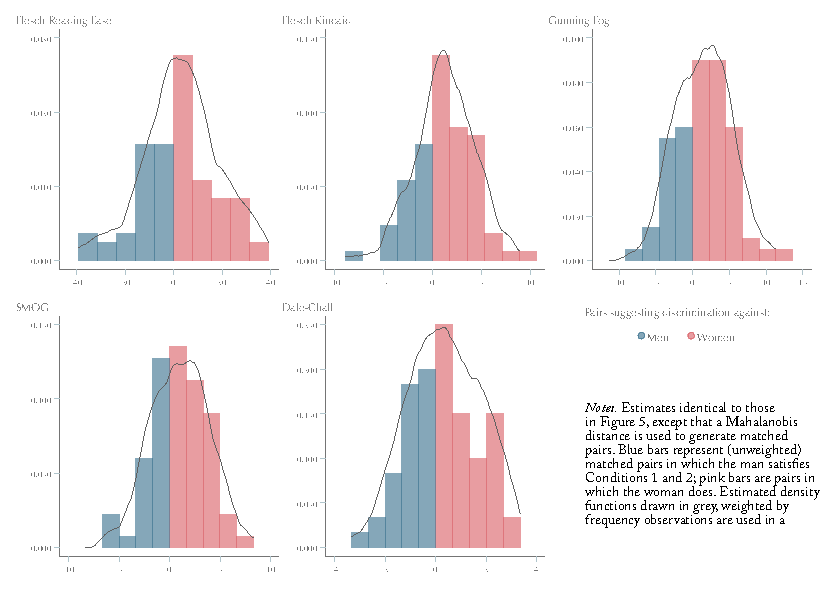
\includegraphics[width=12.3cm]{$HOME/Dropbox/Readability/draft/pdf/figure4XA.pdf}
	}
\end{figure}

\begin{ThreePartTable}
    \begin{TableNotes}
        \tiny\item \textit{Notes}. Table lists the names of the matched pairs from replicating the analysis in Figure 5 but using Mahalanobis matching to match authors. In each panel, female members are listed first; male members second.
    \end{TableNotes}
    {\scriptsize\begin{longtable}[c]{llll}
        \caption{Mahalanobis matching, list of matched pairs}\label{tableC14XA} \\
        \toprule
        \multicolumn{2}{c}{Matched pairs}&\multicolumn{2}{c}{Matched pairs}\\\cmidrule(lr){1-2}\cmidrule(lr){3-4}Female&Male&Female&Male \\
        \midrule
        \endfirsthead
        \multicolumn{4}{c}{\normalsize{\tablename~\thetable{} (continued)}} \\
        \toprule
        \multicolumn{2}{c}{Matched pairs}&\multicolumn{2}{c}{Matched pairs}\\\cmidrule(lr){1-2}\cmidrule(lr){3-4}Female&Male&Female&Male \\
        \midrule
        \endhead
        \midrule
        \endfoot
        \bottomrule
        \insertTableNotes
        \endlastfoot
            Abraham, Katharine G.&Bhattacharya, Sudipto&Kuziemko, Ilyana&Mahoney, Neale\\
            Admati, Anat R.&Huang, Chi-Fu&La Ferrara, Eliana&Krebs, Tom\\
            Amiti, Mary&Koren, Miklós&Landes, Elisabeth M.&Carlton, Dennis W.\\
            Anderson, Siwan&Krebs, Tom&Levy, Gilat&Razin, Ronny\\
            Ashraf, Nava&Ostrovsky, Michael&Lewis, Karen K.&Quah, Danny\\
            Athey, Susan&Haile, Philip A.&Li, Wei&Roland, Gérard\\
            Baicker, Katherine&McClellan, Mark B.&Lleras-Muney, Adriana&Svensson, Jakob\\
            Bailey, Martha J.&Paserman, M. Daniele&Løken, Katrine Vellesen&Carneiro, Pedro\\
            Bandiera, Oriana&Barankay, Iwan&Madrian, Brigitte C.&Smith, Jeffrey\\
            Barwick, Panle Jia&Kennan, John&Maestas, Nicole&Lefgren, Lars\\
            Baxter, Marianne&Backus, David K.&Malmendier, Ulrike&Agarwal, Sumit\\
            Bedard, Kelly&Lefgren, Lars&Matzkin, Rosa L.&McLennan, Andrew\\
            Bertrand, Marianne&Mullainathan, Sendhil&McConnell, Sheena&LaLonde, Robert J.\\
            Black, Sandra E.&Salvanes, Kjell G.&McGrattan, Ellen R.&Williams, Noah\\
            Blank, Rebecca M.&Laband, David N.&Meyer, Margaret A.&Holtz-Eakin, Douglas\\
            Boustan, Leah Platt&Abramitzky, Ran&Molinari, Francesca&Abrevaya, Jason\\
            Brown, Jennifer&Vogel, Jonathan&Moser, Petra&Sunde, Uwe\\
            Busse, Meghan R.&Zettelmeyer, Florian&Nakamura, Emi&Steinsson, Jón\\
            Case, Anne C.&Taylor, Curtis R.&Ng, Serena&Jansson, Michael\\
            Casella, Alessandra&Glazer, Jacob&Niederle, Muriel&Wolfers, Justin\\
            Chen, Xiaohong&Hahn, Jinyong&Oster, Emily&Soares, Rodrigo R.\\
            Chen, Yan&Bolton, Gary E.&Pande, Rohini&Donald, Stephen G.\\
            Chevalier, Judith A.&Lamont, Owen A.&Paxson, Christina H.&Parente, Stephen L.\\
            Chichilnisky, Graciela&Sobel, Joel&Perrigne, Isabelle&Evans, Robert\\
            Correia, Isabel&Nicolini, Juan Pablo&Piazzesi, Monika&Schneider, Martin\\
            Costa, Dora L.&Kahn, Matthew E.&Qian, Nancy&Ok, Efe A.\\
            Cropper, Maureen L.&Halvorsen, Robert&Quinzii, Martine&Magill, Michael J. P.\\
            Currie, Janet&Lavy, Victor&Ramey, Valerie A.&Bresnahan, Timothy F.\\
            Dafny, Leemore S.&Kolstad, Jonathan T.&Reinganum, Jennifer F.&Farrell, Joseph\\
            De Nardi, Mariacristina&Neal, Derek A.&Reinhart, Carmen M.&Taylor, Alan M.\\
            Demange, Gabrielle&Anderson, Robert M.&Rey, Hélène&Jeanne, Olivier\\
            Duflo, Esther&Burgess, Robin&Romer, Christina D.&Ball, Laurence\\
            Dupas, Pascaline&Heffetz, Ori&Rose-Ackerman, Susan&Bhattacharya, Sudipto\\
            Dynan, Karen E.&Kocherlakota, Narayana R.&Rose, Nancy L.&Snyder, James M. (Jr.)\\
            Eberly, Janice C.&Woodford, Michael&Rosenblat, Tanya S.&Möbius, Markus M.\\
            Eckel, Catherine C.&Dufwenberg, Martin&Rouse, Cecilia Elena&Weil, Philippe\\
            Edlund, Lena&Wolfers, Justin&Sapienza, Paola&Spolaore, Enrico\\
            Eyigungor, Burcu&Koren, Miklós&Schennach, Susanne M.&Hong, Han\\
            Fan, Yanqin&Sherman, Robert P.&Schmitt-Grohé, Stephanie&Leeper, Eric M.\\
            Fernández, Raquel&Paserman, M. Daniele&Schwartz, Nancy L.&Nadiri, Mohammed Ishaq\\
            Field, Erica&Donald, Stephen G.&Shannon, Chris&Schmedders, Karl\\
            Finkelstein, Amy&Einav, Liran&Shaw, Kathryn L.&Holtz-Eakin, Douglas\\
            Flavin, Marjorie A.&Lucas, Robert E. B.&Spier, Kathryn E.&Farrell, Joseph\\
            Forges, Françoise&Banks, Jeffrey S.&Stokey, Nancy L.&Smith, Bruce D.\\
            Fortin, Nicole M.&Hyslop, Dean R.&Tenreyro, Silvana&Rubio-Ramírez, Juan F.\\
            Freund, Caroline&Rose, Andrew K.&Tertilt, Michèle&Doepke, Matthias\\
            Fuchs-Schündeln, Nicola&Abadie, Alberto&Tesar, Linda L.&Backus, David K.\\
            Garfinkel, Michelle R.&Bertola, Giuseppe&Thomas, Julia K.&Khan, Aubhik\\
            Goldberg, Pinelopi Koujianou&Levinsohn, James A.&Todd, Petra E.&Flinn, Christopher J.\\
            Goldin, Claudia D.&Abramitzky, Ran&Vissing-Jørgense, Annette&Veronesi, Pietro\\
            Gopinath, Gita&Itskhoki, Oleg&Voena, Alessandra&Aaronson, Daniel\\
            Griffith, Rachel&Hobijn, Bart&Washington, Ebonya L.&Kopczuk, Wojciech\\
            Guerrieri, Veronica&Khan, Aubhik&White, Lucy&Razin, Ronny\\
            Hanna, Rema&Foster, Andrew D.&Whited, Toni M.&Pástor, Ľuboš\\
            Hastings, Justine S.&Callander, Steven&Williams, Heidi L.&Budish, Eric\\
            Ho, Katherine&Kremer, Ilan&Wooders, Myrna Holtz&McLean, Richard P.\\
            Hoxby, Caroline Minter&Kessler, Daniel P.&Yariv, Leeat&Szentes, Balázs\\
            İmrohoroğlu, Ayşe&Casari, Marco&Yellen, Janet L.&Azariadis, Costas\\
            Jayachandran, Seema&Caselli, Francesco&Zeiler, Kathryn&van Soest, Arthur\\
            Kowalski, Amanda E.&Mahoney, Neale&Zhuravskaya, Ekaterina&Francois, Patrick\\
            Kranton, Rachel E.&Baye, Michael R.&&\\
    \end{longtable}}
\end{ThreePartTable}


\clearpage

\section{Male effects []}
\label{maleeffects}

\subsection{\autoref{table4}, journal and male effects}
\label{appendixarticlemale}

\autoref{tableC2} shows male effects from the regressions described and presented in \autoref{table4}. Effects estimated at a female ratio of zero and observed values for other co-variates. Grade-level effects (Flesch-Kincaid, Gunning Fog, SMOG and Dale-Chall) have been multiplied by negative one (\autoref{measuringreadability}). \autoref{tableC3} shows the coefficients on the journal dummies in column (2), \autoref{table4}. They compare \emph{AER}'s readability to the readability of \emph{Econometrica}, \emph{JPE} and \emph{QJE}.

\begin{table}[H]
    \footnotesize
    \centering
    \begin{threeparttable}
        \caption{\autoref{table4}, male effects}
        \label{tableC2}
        \begin{tabular}{p{2.64cm}S@{}S@{}S@{}S@{}S@{}S@{}S@{}}
            \toprule
            &{(1)}&{(2)}&{(3)}&{(4)}&{(5)}&{(6)}&{(7)}\\
            \midrule
            \mrow{3cm}{Flesch Reading Ease}&       0.000&       0.000&       0.000&       0.000&       0.000&      -0.764&      40.291\\
                                          &     (0.000)&     (0.000)&     (0.000)&     (0.000)&     (0.000)&     (0.668)&     (0.086)\\
            \mrow{3cm}{Flesch-Kincaid}    &       0.000&       0.000&       0.000&       0.000&       0.000&      -0.111&     -13.459\\
                                          &     (0.000)&     (0.000)&     (0.000)&     (0.000)&     (0.000)&     (0.147)&     (0.017)\\
            \mrow{3cm}{Gunning Fog}       &       0.000&       0.000&       0.000&       0.000&       0.000&      -0.088&     -17.121\\
                                          &     (0.000)&     (0.000)&     (0.000)&     (0.000)&     (0.000)&     (0.203)&     (0.020)\\
            \mrow{3cm}{SMOG}              &       0.000&       0.000&       0.000&       0.000&       0.000&      -0.069&     -15.065\\
                                          &     (0.000)&     (0.000)&     (0.000)&     (0.000)&     (0.000)&     (0.137)&     (0.015)\\
            \mrow{3cm}{Dale-Chall}        &       0.000&       0.000&       0.000&       0.000&       0.000&      -0.000&     -11.028\\
                                          &     (0.000)&     (0.000)&     (0.000)&     (0.000)&     (0.000)&     (0.065)&     (0.008)\\
            \midrule
            Editor effects                &           {\ding{51}}&           {\ding{51}}&           {\ding{51}}&           {\ding{51}}&           {\ding{51}}&           {\ding{51}}&           {\ding{51}}\\
            Journal effects               &           {\ding{51}}&           {\ding{51}}&           {\ding{51}}&           {\ding{51}}&           {\ding{51}}&           {\ding{51}}&           {\ding{51}}\\
            Year effects                  &            &           {\ding{51}}&           {\ding{51}}&           {\ding{51}}&           {\ding{51}}&           {\ding{51}}&           {\ding{51}}\\
            Journal\(\times\)Year effects          &            &            &           {\ding{51}}&           {\ding{51}}&           {\ding{51}}&           {\ding{51}}&           {\ding{51}}\\
            Institution effects           &            &            &            &           {\ding{51}}&           {\ding{51}}&           {\ding{51}}&           {\ding{51}}\\
            Quality controls              &            &            &            &            &          {\(\text{\ding{51}}^1\)}&          {\(\text{\ding{51}}^1\)}&          {\(\text{\ding{51}}^1\)}\\
            Native speaker                &            &            &            &            &           {\ding{51}}&           {\ding{51}}&           {\ding{51}}\\
            \textit{JEL} (primary) effects&            &            &            &            &            &           {\ding{51}}&            \\
            \textit{JEL} (tertiary) effects&            &            &            &            &            &            &           {\ding{51}}\\
            \bottomrule
        \end{tabular}
        \begin{tablenotes}
            \tiny
            \item \textit{Notes}. 9,121 articles in (1)--(5); 4,993 articles in (6); 5,777 articles---including 561 from \textit{AER Papers \& Proceedings} (see~\autoref{footnote34})---in (7). Figures correspond to the male effects from regression results presented in~\autoref{table4}. Effects estimated at a female ratio of zero and observed values for other co-variates. Quality controls denoted by \(\text{\ding{51}}^1\) include citation count and \(\text{max. }T_j\) fixed effects. Standard errors clustered on editor in parentheses.
        \end{tablenotes}
    \end{threeparttable}
\end{table}

\begin{table}[H]
    \footnotesize
    \centering
    \begin{threeparttable}
        \caption{Journal readability, comparisons to \textit{AER}}
        \label{tableC3}
        \begin{tabular}{p{2cm}S@{}S@{}S@{}S@{}S@{}}
            \toprule
            &{\crcell[b]{Flesch\\[-0.1cm]Reading\\[-0.1cm]Ease}}&{\crcell[b]{Flesch-\\[-0.1cm] Kincaid}}&{\crcell[b]{Gunning\\[-0.1cm]Fog}}&{SMOG}&{\crcell[b]{Dale-\\[-0.1cm]Chall}}\\
            \midrule
            \textit{Econometrica}         &      -12.48***&       -4.44***&       -4.26***&       -2.63***&       -0.66***\\
                                          &      (1.93)   &      (0.41)   &      (0.47)   &      (0.38)   &      (0.16)   \\
            \textit{JPE}                  &       -5.69***&       -4.01***&       -3.42***&       -1.84***&        0.18   \\
                                          &      (1.93)   &      (0.41)   &      (0.47)   &      (0.38)   &      (0.16)   \\
            \textit{QJE}                  &        1.47** &       -0.04   &        0.28***&        0.19***&        0.27***\\
                                          &      (0.63)   &      (0.14)   &      (0.09)   &      (0.07)   &      (0.05)   \\
            \bottomrule
        \end{tabular}
        \begin{tablenotes}
            \tiny
            \item \textit{Notes}. Figures are the estimated coefficients on the journal dummy variables from (2) in~\autoref{table4}. Each contrasts the readability of the journals in the left-hand column with the readability of \textit{AER}. Standard errors clustered on editor in parentheses. ***, ** and * statistically significant at 1\%, 5\% and 10\%, respectively.
        \end{tablenotes}
    \end{threeparttable}
\end{table}

\clearpage

\subsection{\autoref{table5}, male effects}
\label{appendixauthormale}

\autoref{tableC4} displays total male effects---\emph{i.e.}, the total effect for men co-authoring only with other men---from the regressions presented in \autoref{table5}. Effects estimated at a female ratio of zero and observed values for other co-variates. Grade-level effects (Flesch-Kincaid, Gunning Fog, SMOG and Dale-Chall) have been multiplied by negative one (see \autoref{measuringreadability}).

\begin{table}[H]
    \footnotesize
    \centering
    \begin{threeparttable}
        \caption{\autoref{table5}, male effects}
        \label{tableC4}
        \begin{tabular}{p{4cm}S@{}S@{}S@{}S@{}S@{}}
            \toprule
            &{\crcell[b]{Flesch\\[-0.1cm]Reading\\[-0.1cm]Ease}}&{\crcell[b]{Flesch-\\[-0.1cm] Kincaid}}&{\crcell[b]{Gunning\\[-0.1cm]Fog}}&{SMOG}&{\crcell[b]{Dale-\\[-0.1cm]Chall}}\\
            \midrule
            \mrow{4cm}{Male effect}       &      39.727&     -13.634&     -17.367&     -15.288&     -11.006\\
                                          &     (0.146)&     (0.033)&     (0.037)&     (0.027)&     (0.012)\\
            \midrule
            \(N_j\)              &           {\ding{51}}&           {\ding{51}}&           {\ding{51}}&           {\ding{51}}&           {\ding{51}}\\
            Editor effects                &           {\ding{51}}&           {\ding{51}}&           {\ding{51}}&           {\ding{51}}&           {\ding{51}}\\
            Journal effects               &           {\ding{51}}&           {\ding{51}}&           {\ding{51}}&           {\ding{51}}&           {\ding{51}}\\
            Year effects                  &           {\ding{51}}&           {\ding{51}}&           {\ding{51}}&           {\ding{51}}&           {\ding{51}}\\
            Journal\(\times\)Year effects          &           {\ding{51}}&           {\ding{51}}&           {\ding{51}}&           {\ding{51}}&           {\ding{51}}\\
            Institution effects           &           {\ding{51}}&           {\ding{51}}&           {\ding{51}}&           {\ding{51}}&           {\ding{51}}\\
            Quality controls              &          {\(\text{\ding{51}}^1\)}&          {\(\text{\ding{51}}^1\)}&          {\(\text{\ding{51}}^1\)}&          {\(\text{\ding{51}}^1\)}&          {\(\text{\ding{51}}^1\)}\\
            Native speaker                &           {\ding{51}}&           {\ding{51}}&           {\ding{51}}&           {\ding{51}}&           {\ding{51}}\\
            \bottomrule
        \end{tabular}
        \begin{tablenotes}
            \tiny
            \item \textit{Notes}. Sample 9,186 observations (2,827 authors). Figures correspond to the male effects from regression results presented in~\autoref{table5} (first-differenced, IV estimation of~\autoref{equation1}, ~\citet{Arellano1995,Blundell1998}). Effects estimated at a female ratio of zero and observed values for other co-variates. Quality controls denoted by \(\text{\ding{51}}^1\) include citation count and \(\text{max. }T_j\) fixed effects. Regressions weighted by \(1/N_j\); standard errors adjusted for two-way clustering on editor and author (in parentheses).
        \end{tablenotes}
    \end{threeparttable}
\end{table}

\clearpage

\subsection{\autoref{table10}, male effects []}
\label{maleeffects}

\autoref{tableC17} shows $\widehat R_{k3}$ for men in the matched sample. Grade-level effects (Flesch-Kincaid, Gunning Fog, SMOG and Dale-Chall) have been multiplied by negative one (\autoref{measuringreadability}).

\begin{table}[H]
    \footnotesize
    \centering
    \begin{threeparttable}
        \caption{Mean \(\widehat R_{k3}\) (men)}
        \label{tableC17}
        \begin{tabular}{p{3cm}S@{}S@{}S@{}S@{}S@{}}
            \toprule
            &{\crcell[b]{Flesch\\[-0.1cm]Reading\\[-0.1cm]Ease}}&{\crcell[b]{Flesch-\\[-0.1cm] Kincaid}}&{\crcell[b]{Gunning\\[-0.1cm]Fog}}&{SMOG}&{\crcell[b]{Dale-\\[-0.1cm]Chall}}\\
            \midrule
            \(\widehat R_{k3}\) (men)     &      37.194&     -15.094&     -18.568&     -15.618&     -11.264\\
                                          &     (1.048)&     (0.279)&     (0.293)&     (0.193)&     (0.087)\\
            \bottomrule
        \end{tabular}
        \begin{tablenotes}
            \tiny
            \item \textit{Notes}. Sample 121 matched pairs (106 and 121 distinct men and women, respectively). Figures correspond to the \(t=3\) reconstructed readability scores for men. \(\widehat R_{i3}\) weighted by frequency observations are used in a match; degrees-of-freedom corrected standard errors in parentheses.
        \end{tablenotes}
    \end{threeparttable}
\end{table}
  

## [](#table8), male effects [] ##




[](#tableC7) shows male effects from the regressions described and presented in [](#table8). Effects estimated at a female ratio of zero and observed values for other co-variates. Grade-level effects (Flesch-Kincaid, Gunning Fog, SMOG and Dale-Chall) have been multiplied by [negative one][MeasuringReadability].

<!--\begin{table}[H]
    \footnotesize
    \centering
    \begin{threeparttable}
        \caption{\autoref{table8}, male effects}
        \label{tableC7}
        \begin{tabular}{p{3cm}S@{}S@{}S@{}S@{}S@{}S@{}S@{}}
            \toprule
            &{\(t=1\)}&{\(t=2\)}&{\(t=3\)}&{\(t=4\text{--}5\)}&{\(t\ge6\)}&{All}\\
            \midrule
            Flesch Reading Ease           &      39.578&      39.552&      39.644&      39.589&      39.837&      39.715\\
                                          &     (0.060)&     (0.106)&     (0.145)&     (0.146)&     (0.204)&     (0.149)\\
            Flesch-Kincaid                &     -13.714&     -13.689&     -13.653&     -13.640&     -13.586&     -13.650\\
                                          &     (0.012)&     (0.023)&     (0.030)&     (0.032)&     (0.042)&     (0.035)\\
            Gunning Fog                   &     -17.431&     -17.402&     -17.362&     -17.357&     -17.280&     -17.382\\
                                          &     (0.015)&     (0.027)&     (0.036)&     (0.038)&     (0.052)&     (0.038)\\
            SMOG                          &     -15.253&     -15.244&     -15.229&     -15.233&     -15.184&     -15.242\\
                                          &     (0.011)&     (0.020)&     (0.026)&     (0.027)&     (0.037)&     (0.026)\\
            Dale-Chall                    &     -11.018&     -11.031&     -11.026&     -11.045&     -11.025&     -11.008\\
                                          &     (0.006)&     (0.008)&     (0.011)&     (0.011)&     (0.015)&     (0.012)\\
            \midrule
            No. observations              &       6,876&       2,827&       1,674&       1,908&       2,777&      12,013\\
            \(N_j\)                       &           {\ding{51}}&           {\ding{51}}&           {\ding{51}}&           {\ding{51}}&           {\ding{51}}&           {\ding{51}}\\
            Editor effects                &           {\ding{51}}&           {\ding{51}}&           {\ding{51}}&           {\ding{51}}&           {\ding{51}}&           {\ding{51}}\\
            Journal effects               &           {\ding{51}}&           {\ding{51}}&           {\ding{51}}&           {\ding{51}}&           {\ding{51}}&           {\ding{51}}\\
            Year effects                  &           {\ding{51}}&           {\ding{51}}&           {\ding{51}}&           {\ding{51}}&           {\ding{51}}&           {\ding{51}}\\
            Journal\(\times\)Year effects          &            &            &            &            &            &           {\ding{51}}\\
            Institution effects           &           {\ding{51}}&           {\ding{51}}&           {\ding{51}}&           {\ding{51}}&           {\ding{51}}&           {\ding{51}}\\
            Quality controls              &          {\(\text{\ding{51}}^4\)}&          {\(\text{\ding{51}}^4\)}&          {\(\text{\ding{51}}^4\)}&          {\(\text{\ding{51}}^4\)}&          {\(\text{\ding{51}}^4\)}&          {\(\text{\ding{51}}^1\)}\\
            Native speaker                &           {\ding{51}}&           {\ding{51}}&           {\ding{51}}&           {\ding{51}}&           {\ding{51}}&           {\ding{51}}\\
            \bottomrule
        \end{tabular}
        \begin{tablenotes}
            \tiny
            \item \textit{Notes}. Figures correspond to the male effects from regression results presented in~\autoref{table8} (FGLS estimation of ~\autoref{equation1} without lagged dependent variable). First column restricts sample to authors' first publication in the data (\(t=1\)), second column to their second (\(t=2\)), \textit{etc.} Regressions weighted by \(1/N_j\) (see~\autoref{authorlevel}). Standard errors (in parentheses) adjusted for two-way clustering (editor and author) and cross-model correlation. Final column estimates from an unweighted population-averaged regression; error correlations specified by an auto-regressive process of order one and standard errors (in parentheses) adjusted for one-way clustering on author. Quality controls denoted by \(\text{\ding{51}}^1\) include citation count and \(\text{max. }T_j\) fixed effects; \(\text{\ding{51}}^4\) includes citation count, only.
        \end{tablenotes}
    \end{threeparttable}
\end{table}

\clearpage
\printbibheading[heading=subbibintoc]
\printbibliography[segment=0, heading=none]
\end{refsection}

\end{appendices}

\end{document}
